\chapter[Experimentos]{Experimentos}

Os experimentos realizados neste trabalho compreendem os algoritmos NSGA-II [], NSGA-III [], SPEA2 [], MOEA/D [], AEMMT [], AEMMD [], MOACS e o ACO proposto: MACO/D. Todos os métodos são testados em dois problemas discretos multiobjetivos: o PMM e o PRM. A fim  de verificar o comportamento dos algoritmos em relação ao número de objetivos, diversas formulações foram consideradas, avaliando-se problemas desde dois até seis objetivos. Assim como o número de funções objetivos, a topologia da rede (PRM) e a quantidade de itens (PMM) também afetam a complexidade, portanto elaborou-se instâncias diferentes para cada problema: no PRM, considerou-se seis redes de diferentes complexidades e no PMM variou-se a quantidade de itens em 30, 40, 50, 100 e 200.

Os experimentos podem ser divididos em três etapas distintas:

\begin{enumerate}
	\item Teste dos AG's multiobjetivos NSGA-II, NSGA-III, SPEA2, MOEA/D e AEMMT nos problemas da mochila e do roteamento multicast. O número de objetivos varia entre dois e seis e, no PRM, três redes são testadas, enquanto o PMM lida com instâncias de 30, 50 e 100 itens. Esses experimentos compuseram o primeiro artigo gerado neste trabalho intitulado \textit{``A Comparative Analysis of MOEAs Considering Two Discrete Optimization Problems''} [], em português, uma análise comparativa entre algoritmos evolutivos multiobjetivos considerando dois problemas de otimização discretos. Além dos cinco algoritmos mencionados, avalia-se também uma pequena modificação no AEMMT chamada de AEMMT-f que remove o limite no tamanho do arquivo de soluções não-dominadas. As avaliações dos algoritmos são feitas com base em métricas relacionadas ao Pareto conhecido e permitem um melhor entendimento sobre o comportamento dos algoritmos, o que facilita a identificação de pontos fortes e fracos de cada estratégia, ajudando na elaboração de um novo modelo melhor adequado aos problemas em questão (PMM e PRM).
	\item Teste dos métodos de otimização many-objective NSGA-III, MOEA/D, AEMMT, AEMMD e do algoritmo proposto, MACO/D, nos problemas da mochila e do roteamento multicast. São testadas formulações com 4, 5 e 6 objetivos, avaliando-se 3 redes no PRM e problemas com 30, 40 e 50 itens no PMM. Esses experimentos foram responsáveis pela publicação do segundo artigo intitulado \textit{``MACO/D: Many-objective Ant Colony Optimization based on Decomposed Pheromone''} [], em português, MACO/D: otimização por colônia de formigas com muitos objetivos baseada em decomposição de feromônios. Os experimentos colocam à prova pela primeira vez o algoritmo proposto neste trabalho e revelam suas vantagens e fraquezas, possibilitando a identificação dos casos em que se é uma boa ideia utilizá-lo e as formas em que se pode melhorá-lo em cenários onde que os resultados foram desfavoráveis.
	\item Teste dos algoritmos de otimização many-objective NSGA-III, MOEA/D, AEMMT, AEMMD e MACO/D em instâncias complexas do PMM e PRM utilizando a métrica hipervolume, independente do Pareto. Esses experimentos são necessários, pois as duas etapas anteriores testaram apenas problemas com complexidade razoável onde se é possível estimar o Pareto. A inclusão de mais itens no PMM ou o uso de redes mais complexas no PRM torna inviável a obtenção da fronteira de Pareto e faz necessária a utilização do hipervolume para avaliar os algoritmos. Nesses experimentos são testadas duas novas redes para o PRM e duas novas instâncias do PMM, com 100 e 200 itens.
\end{enumerate}

Considerando as três etapas de experimentos, foram usadas 5 métricas diferentes para se avaliar os algoritmos, são elas:

\begin{itemize}
	\item Taxa de erro ($ER$): porcentagem das soluções encontradas que não fazem parte do Pareto aproximado;
	\item \textit{Generational distance} ($GD$): distância entre das soluções incorretas para a solução mais próxima no Pareto aproximado. Mede o quão distantes as soluções erradas encontradas estão de uma solução correta.
	\item \textit{Pareto subset} ($PS$): número absoluto de soluções encontradas que fazem parte do Pareto aproximado.
	\item Hipervolume ($HV$): Única métrica, além do tempo, utilizada que independe de um Pareto pré-conhecido. Mede o volume da figura geométrica m-dimensional (m é o número de objetivos) formada pelas distâncias entre as soluções encontradas e um ponto de referência $p_{ref}$. As coordenadas de $p_{ref}$ são diferentes para cada cenário (problema, formulação de objetivos e instância) e são determinadas pelo pior valor encontrado em cada um dos objetivos considerando a união das soluções dos Paretos obtidos em cada execução. Se o PMM de 5 objetivos e 100 itens é executado 10 vezes, por exemplo, extrai-se os 10 resultados e coloca-se soluções em um único conjunto $S_{todos}$. Varre-se $S_{todos}$ procurando pelo pior valor em cada uma das 5 coordenadas e cria-se uma solução fictícia $p_{ref}$ para os valores encontrados. $p_{ref}$ é então utilizado como ponto de referência para o PMM de 5 objetivos e 100 itens. Para os experimentos deste trabalho foi utilizada a implementação oficial do cálculo de hipervolume em [].
	\item Tempo: tempo em segundos necessário para se executar o algoritmo.
\end{itemize}

As seções a seguir apresentam os experimentos e seus resultados em cada uma das etapas citadas acima.

\section{Etapa 1: AG's multiobjetivos}

Neste etapa testou-se os algoritmos NSGA-II, NSGA-III, SPEA2, MOEA/D e AEMMT. Ao todo, 30 cenários de teste foram considerados:

\begin{itemize}
	\item PRM: 5 formulações de objetivos ($P_2$, $P_3$, $P_4$, $P_5$ e $P_6$) e 3 redes ($R_1$, $R_2$ e $R_3$). Tanto as formulações quanto às redes foram descritas na seção correspondente ao problema do roteamento multicast [].
	\item PMM: 5 formulações de objetivos (2 a 6) e 3 instâncias (30, 50 e 100 itens).
\end{itemize}

Para cada um dos cenários foi extraído um Pareto através de múltiplas execuções dos 5 algoritmos testados. A tabela \ref{table_exp1_paretos} mostra a cardinalidade de cada Pareto encontrado.

\begin{table}[!htbp]
	\centering
	\caption{Cardinalidade dos Paretos encontrados para a primeira etapa de experimentos}
	\label{table_exp1_paretos}
	\begin{tabular}{c|rrr|rrr}
		& \multicolumn{3}{c|}{\textbf{PRM}} & \multicolumn{3}{c}{\textbf{PMM}} \\ \hline
		Objetivos & R1         & R2       & R3        & 30 itens  & 50 itens & 100 itens \\ \hline
		2         & 14         & 9        & 6         & 15        & 67       & 170       \\
		3         & 30         & 18       & 17        & 106       & 501      & 6288      \\
		4         & 122        & 72       & 60        & 425       & 986      & 88374*    \\
		5         & 424        & 326      & 551       & 1765      & 5213     & 176868*   \\
		6         & 1196       & 657      & 1078      & 5800      & 35760*   & 248198*   \\ \hline
	\end{tabular}
\end{table}

Na tabela \ref{table_exp1_paretos}, a quantidade de elementos nos paretos do PMM é demasiadamente grande para as formulações de objetivos com 100 itens, isso acontece, pois o espaço de busca do problema da mochila cresce exponencialmente com o número de itens. Além disso, a situação é pior quando o número de objetivos é alto, pois, naturalmente, quanto maior a quantidade de funções objetivos, maior o número de soluções que serão não-dominadas. O asterisco ao lado de alguns valores no PMM significa que não foi possível estabilizar o Pareto, ou seja, cada rodada de execuções dos algoritmos encontrava novas soluções. Principalmente por essa razão, julgou-se necessária a execução da etapa 3 de experimentos, onde não se usa um Pareto pré-calculado para se avaliar os algoritmos. Apesar de não serem perfeitos, os resultados para o problema de 100 itens ainda são relevantes, pois ainda que os Paretos não sejam estáveis, compara-se as execuções de todos algoritmos contra as melhores soluções encontradas por todos eles, o que indica o algoritmo com melhor potencial para encontrar boas soluções em problemas multiobjetivos.

Para compilar os resultados através das medidas de desempenho $ER$, $GD$ e $PS$, foram feitas 100 execuções de cada algoritmo com os parâmetros listados na tabela \ref{table_exp1_parametros}. As figuras \ref{fig_exp1_pmm_30}, \ref{fig_exp1_pmm_50} e \ref{fig_exp1_pmm_100} mostram respectivamente os resultados para o PMM de 30, 50 e 100 itens. As figuras \ref{fig_exp1_prm_r1}, \ref{fig_exp1_prm_r2} e \ref{fig_exp1_prm_r3} revelam respectivamente os resultados para o PRM aplicado às redes $R_1$, $R_2$ e $R_3$. Uma análise conjunta, com uma média entre as três instâncias de cada problema é apresenta nas figuras \ref{fig_exp1_prm_todos} (PRM) e \ref{fig_exp1_pmm_todos} (PMM).

\begin{table}[!htbp]
	\caption{Parâmetros utilizados pelos algoritmos no PRM e PMM.}
	\begin{center}
		\begin{tabular}{c|r|r}
			\textbf{Parameter} & \textbf{(A) MRP} &  \textbf{(B) MKP} \\ %\hline
			\hline
			Tamanho da população                    &    90 &      150 \\ %\hline
			Número de gerações*                     &   100 &      100 \\ %\hline
			Taxa de crossover                       & 100\% &    100\% \\ %\hline
			Taxa de mutação                         &  20\% & variável \\ %\hline
			Tamanho da vizinhança (MOEA/D)          &    10 &       10 \\ %\hline
			Tamanho das tabelas (AEMMT)             &    30 &       50 \\ %\hline
			Tamanho da tabela de dominância (MEAMT) &    90 &      150 \\ %\hline
			Número de subdivisões (NSGA-III)        &     8 &        8 \\
			\hline
		\end{tabular}
		\label{tab_Params}
	\end{center}
\end{table}

Na tabela \ref{table_exp1_parametros}, o asterisco em ``número de gerações'' é para dizer que nem todos os algoritmos seguem esse parâmetro. o AEMMT executa 9 mil gerações para o PRM e 7500 para o PMM. Isso acontece, pois esse algoritmo gera apenas 1 filho por ciclo no PRM e apenas 2 no PMM necessitando, portanto, de mais gerações para fazer o mesmo número de comparações. No problema da mochila com 100 itens, devido à complexidade do problema, dobrou-se a quantidade de gerações. Ainda na tabela \ref{table_exp1_parametros}, ``variável'' quer dizer que a taxa de mutação foi de 6\% para o PMM de 30 itens, 4\% para o de 50 itens e 2\% para o de 100 itens, similar aos valores utilizados em [12-Bracis].

\begin{figure*}[!htbp]
	\caption{Etapa 1: resultados para o PMM com 30 itens}
	\label{fig_exp1_mkp_30}
	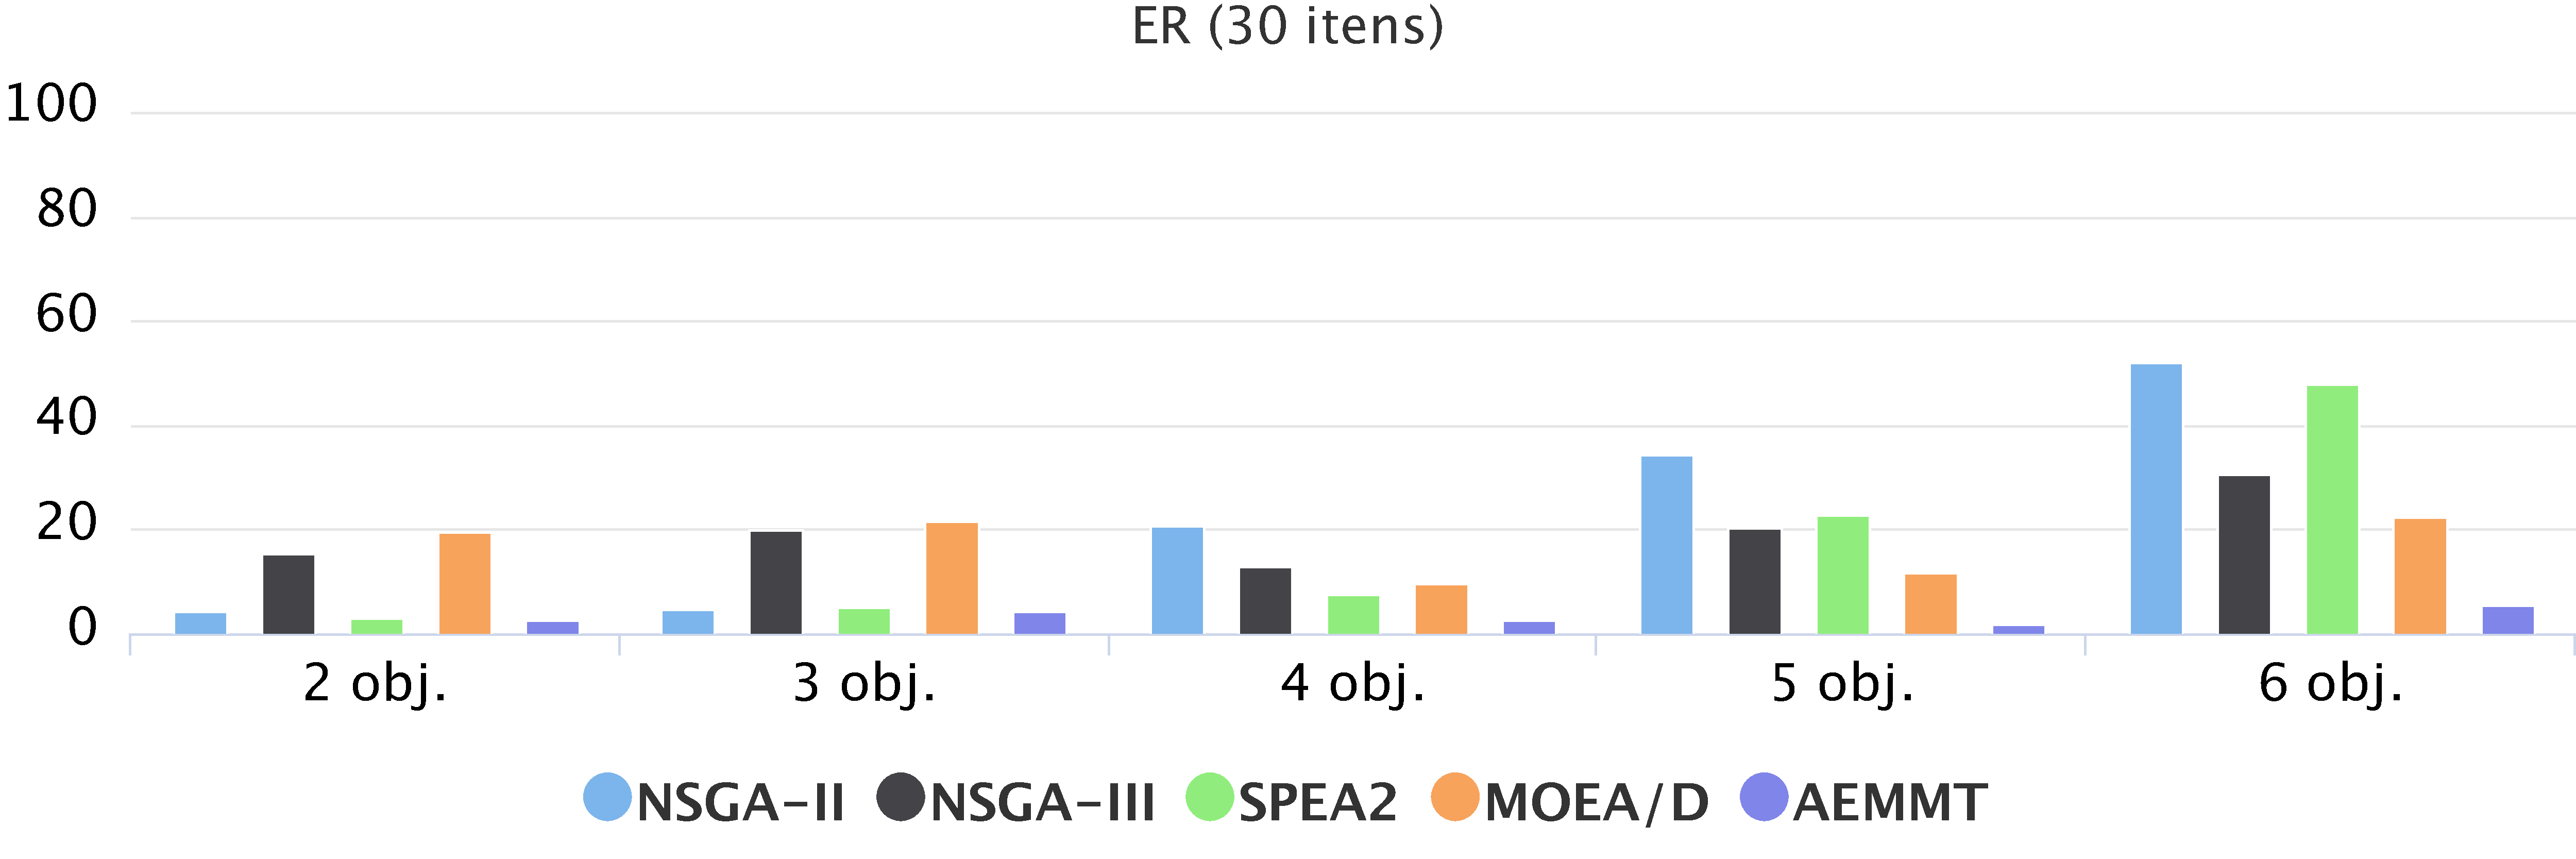
\includegraphics[width=1\textwidth]{cap_experimentos/figs/etapa1/er-mkp-30}
	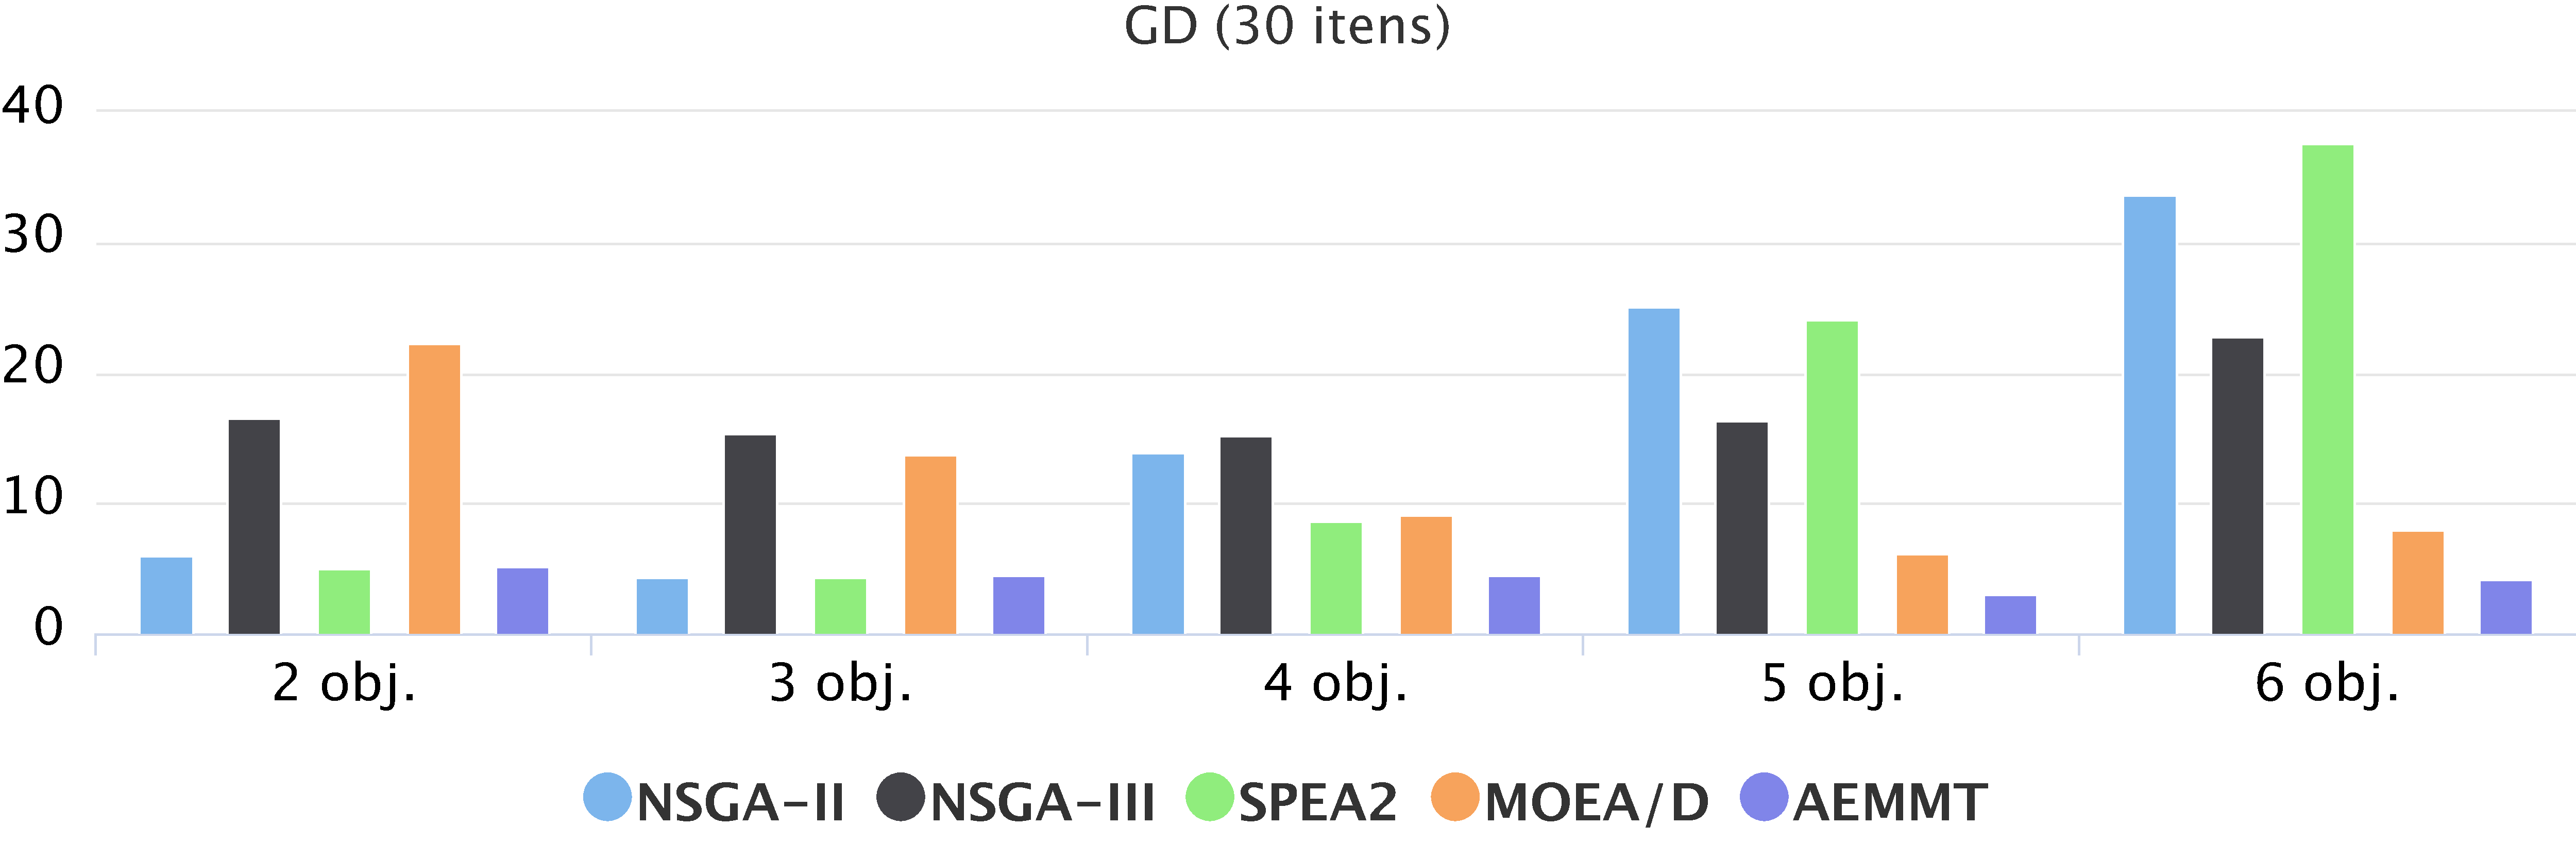
\includegraphics[width=1\textwidth]{cap_experimentos/figs/etapa1/gd-mkp-30}
	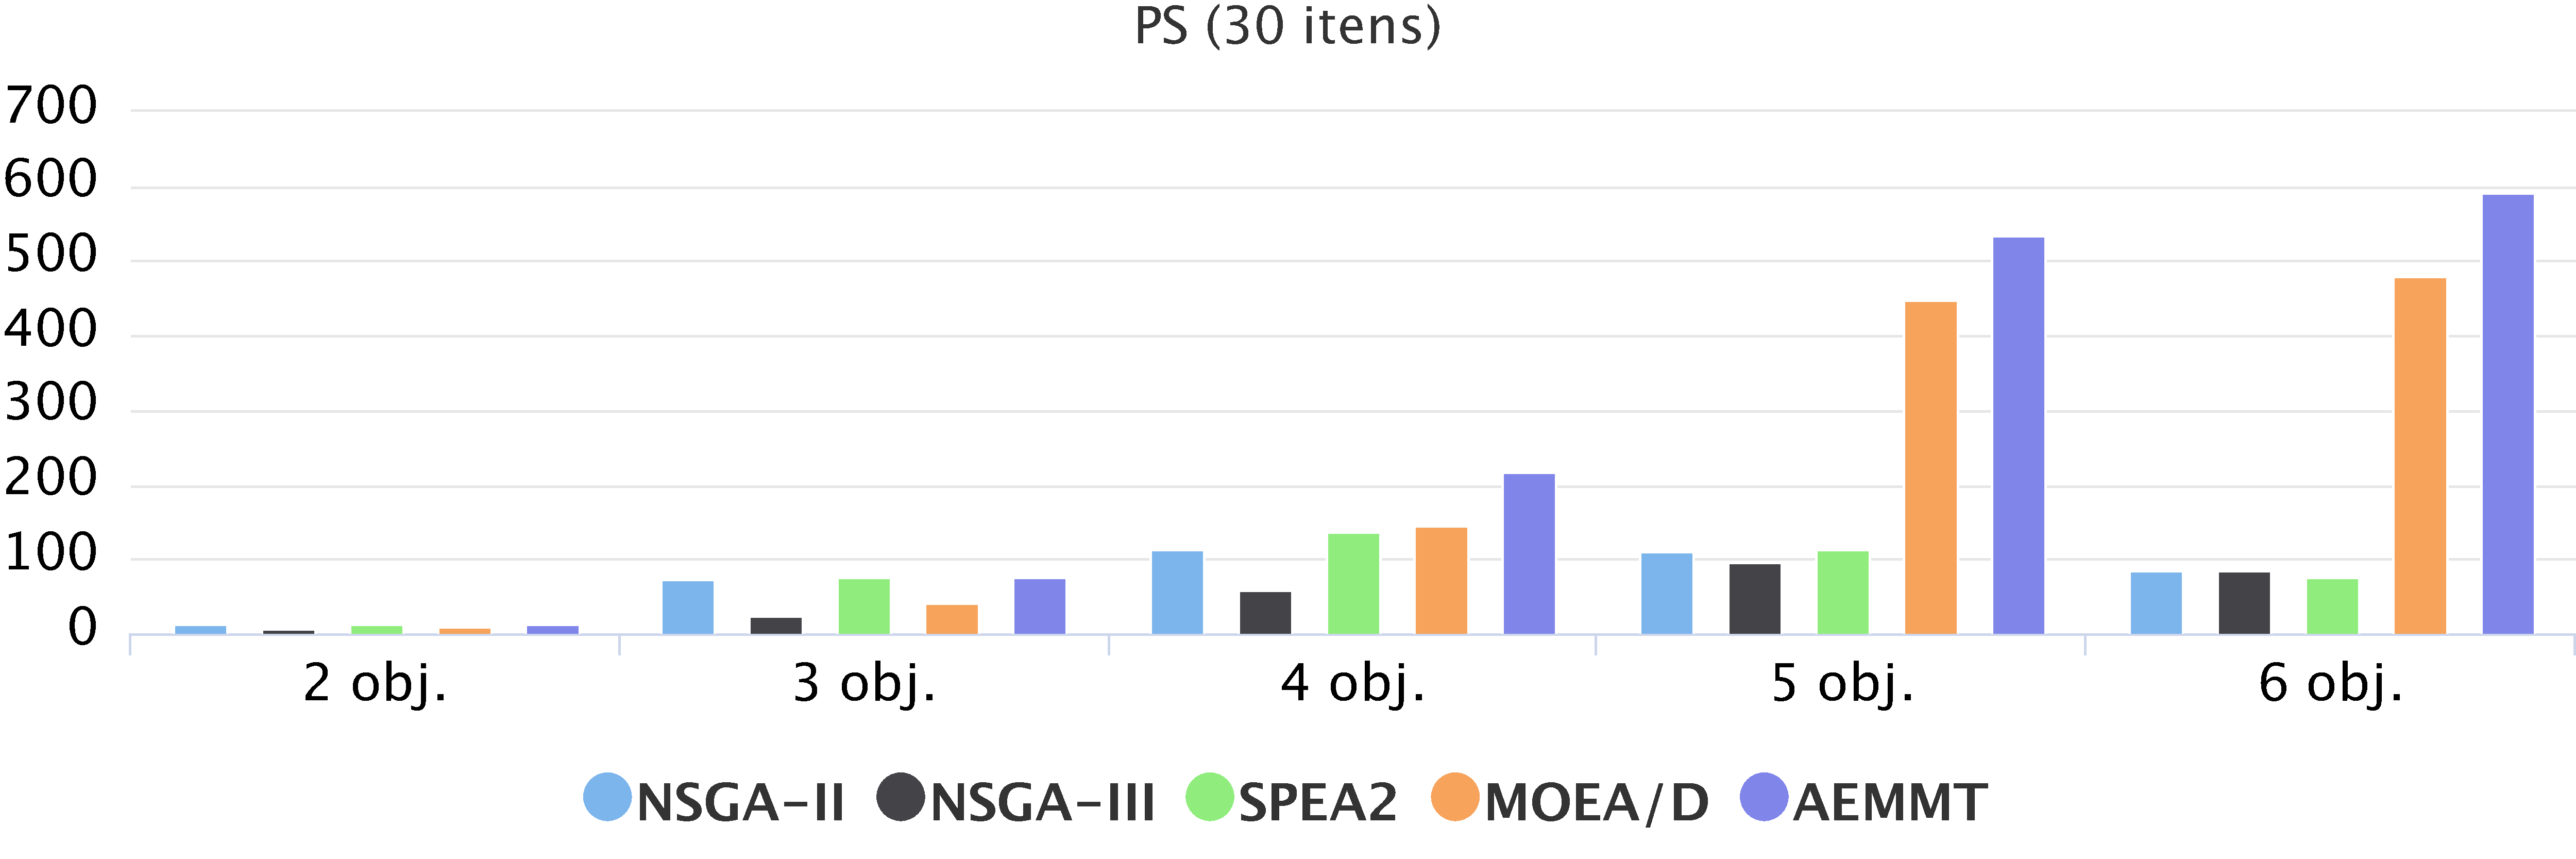
\includegraphics[width=1\textwidth]{cap_experimentos/figs/etapa1/ps-mkp-30}
\end{figure*}

O PMM com 30 itens (figura \ref{fig_exp1_mkp_30}) é um problema simples e geralmente qualquer método de otimização multiobjetivo atinge bons resultados. Até 4 objetivos, apenas o MOEA/D passou a marca de 20\% de erro. Para 2 e 3 objetivos, o NSGA-II, o SPEA2 e o AEMMT são indistinguíveis e possuem erro muito baixo. A partir de 4 objetivos é possível notar uma piora considerável nos algoritmos clássicos NSGA-II e SPEA-2. Considerando todas as formulações de objetivo, os melhores resultados foram obtidos pelo AEMMT que manteve o erro abaixo de 6\% em todos os casos. O $GD$ acompanha as conclusões tiradas a partir do $ER$, o AEMMT gera, globalmente, os melhores resultados enquanto, apesar de terem ótimo desempenho nos problemas de 2 e 3 objetivos, o NSGA-II e o SPEA2 sofrem a partir de 4 objetivos. O tamanho da fronteira de Pareto encontrada, medida pelo $PS$, é maior nos algoritmos MOEA/D e AEMMT, o que é esperado, pois diferentemente dos demais, esses dois algoritmos não aplicam uma limitação muito grande sobre o tamanho do Pareto. Para o PMM de 30 itens está claro que, em qualquer situação, o AEMMT é o melhor dentre os métodos testados.

\begin{figure*}[!htbp]
	\caption{Etapa 1: resultados para o PMM com 50 itens}
	\label{fig_exp1_mkp_50}
	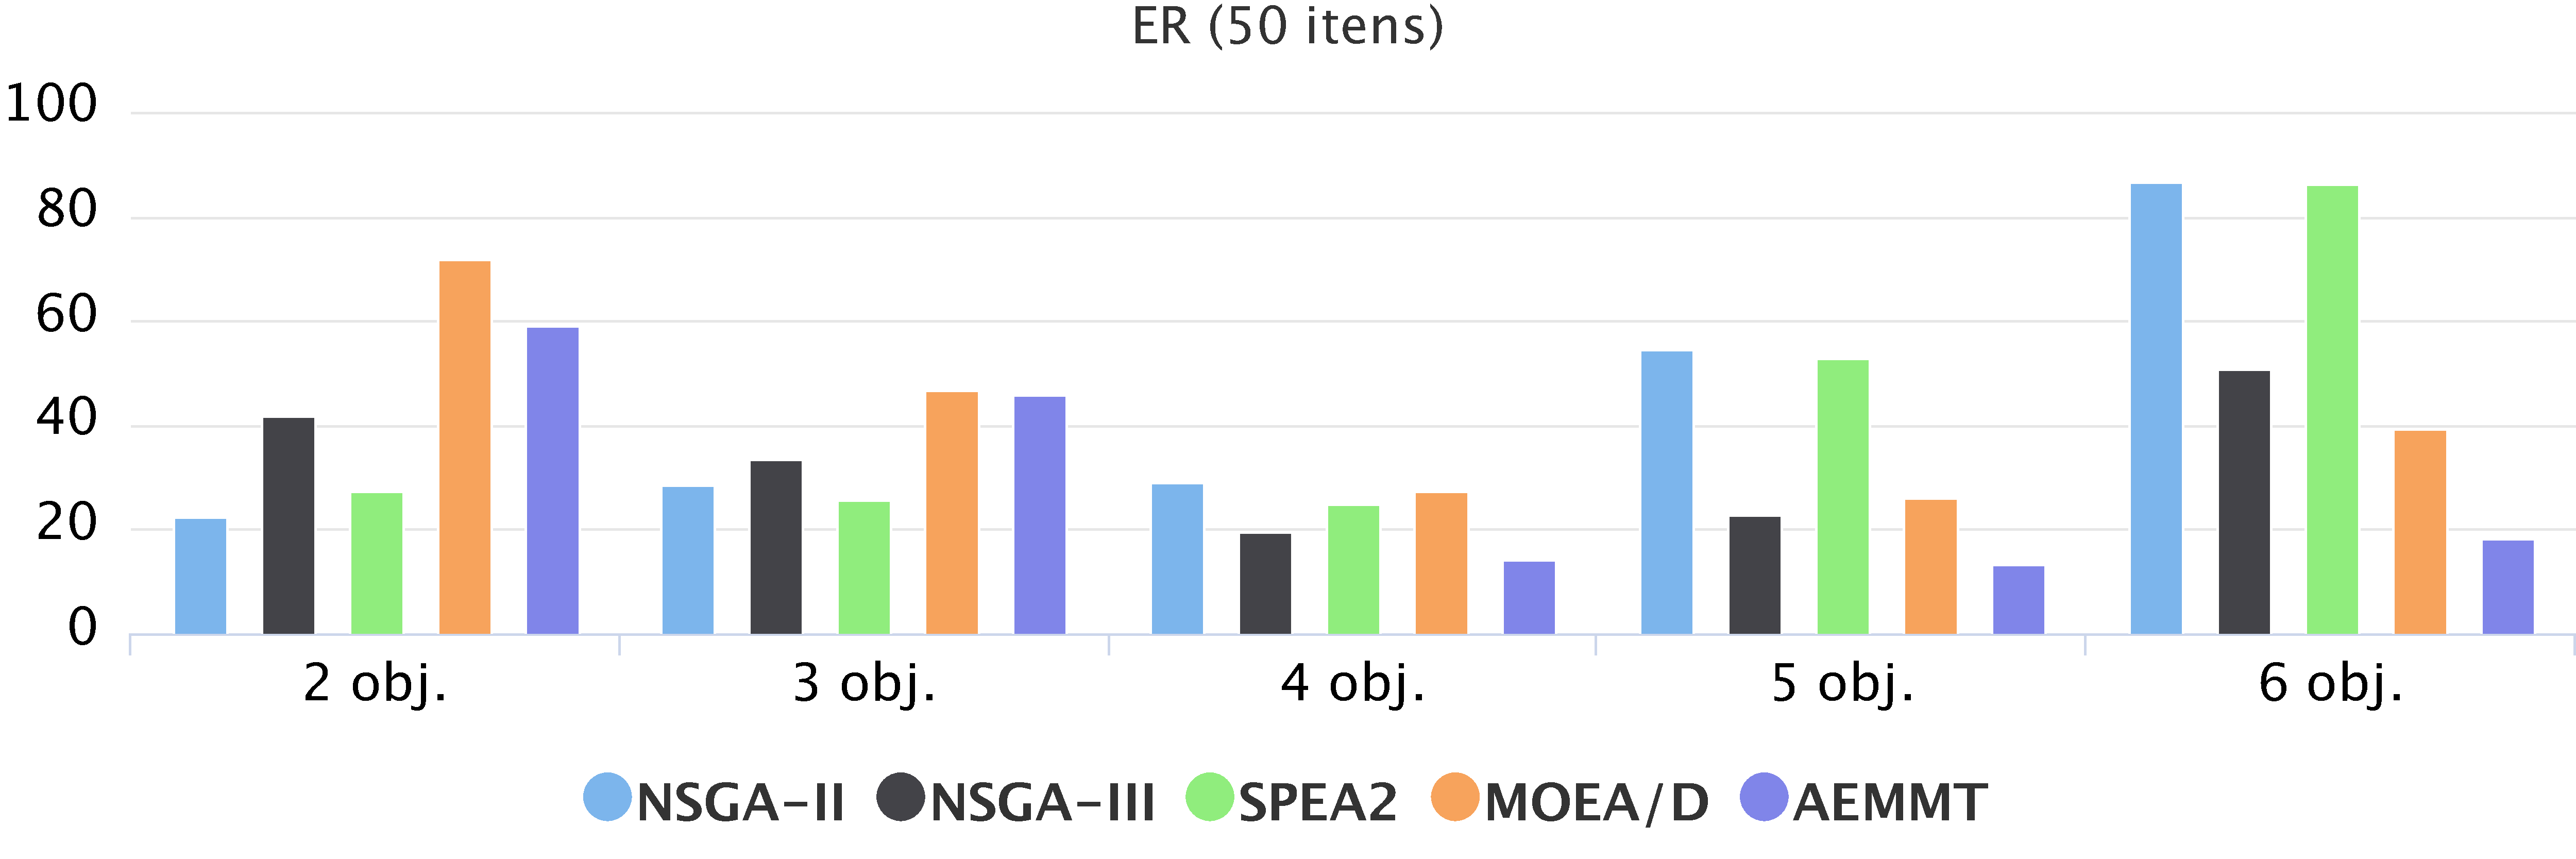
\includegraphics[width=1\textwidth]{cap_experimentos/figs/etapa1/er-mkp-50}
	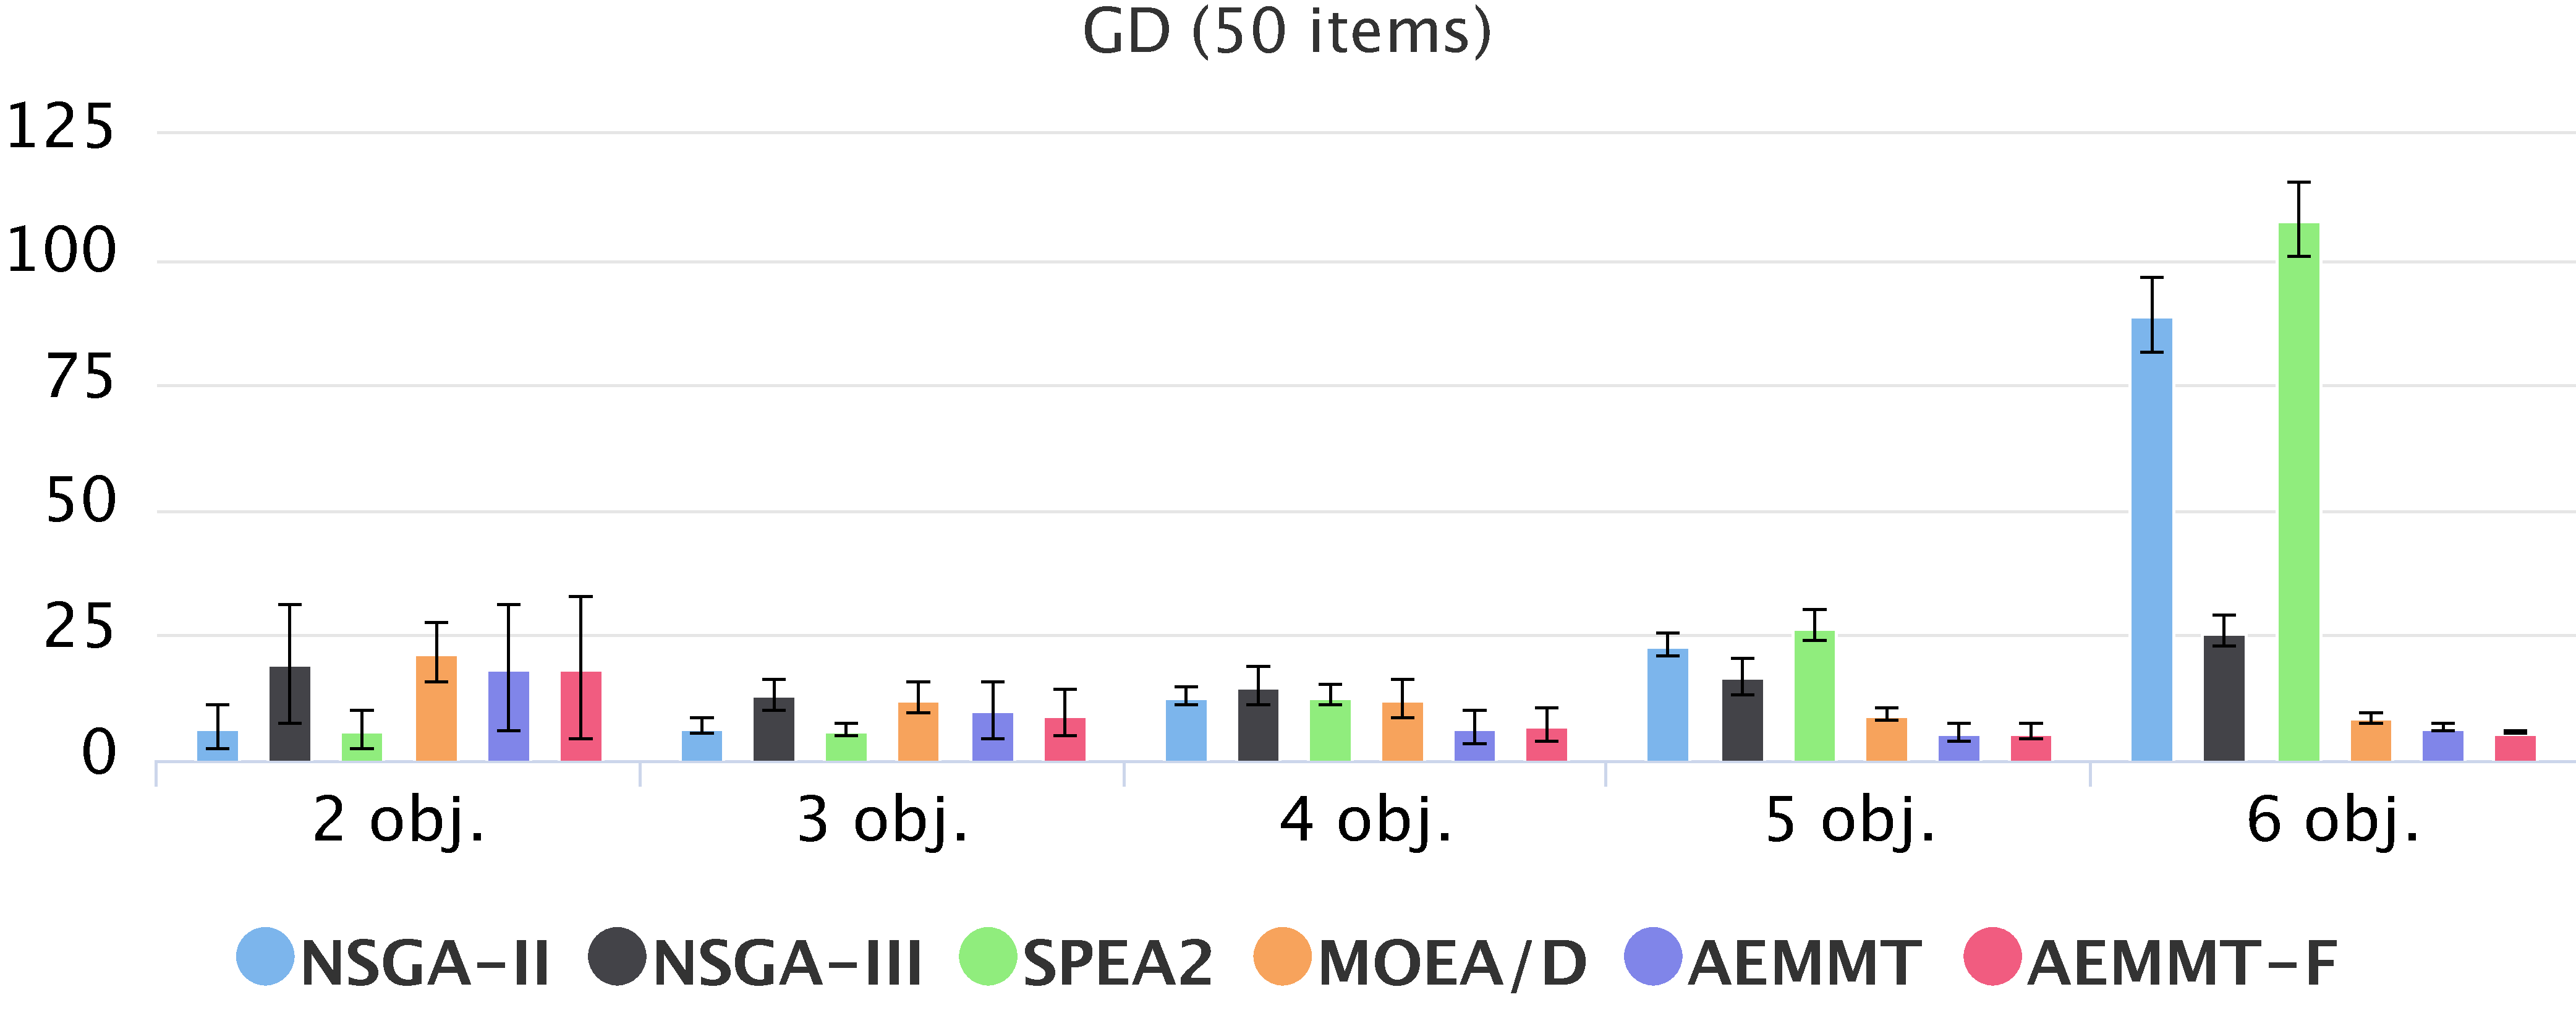
\includegraphics[width=1\textwidth]{cap_experimentos/figs/etapa1/gd-mkp-50}
	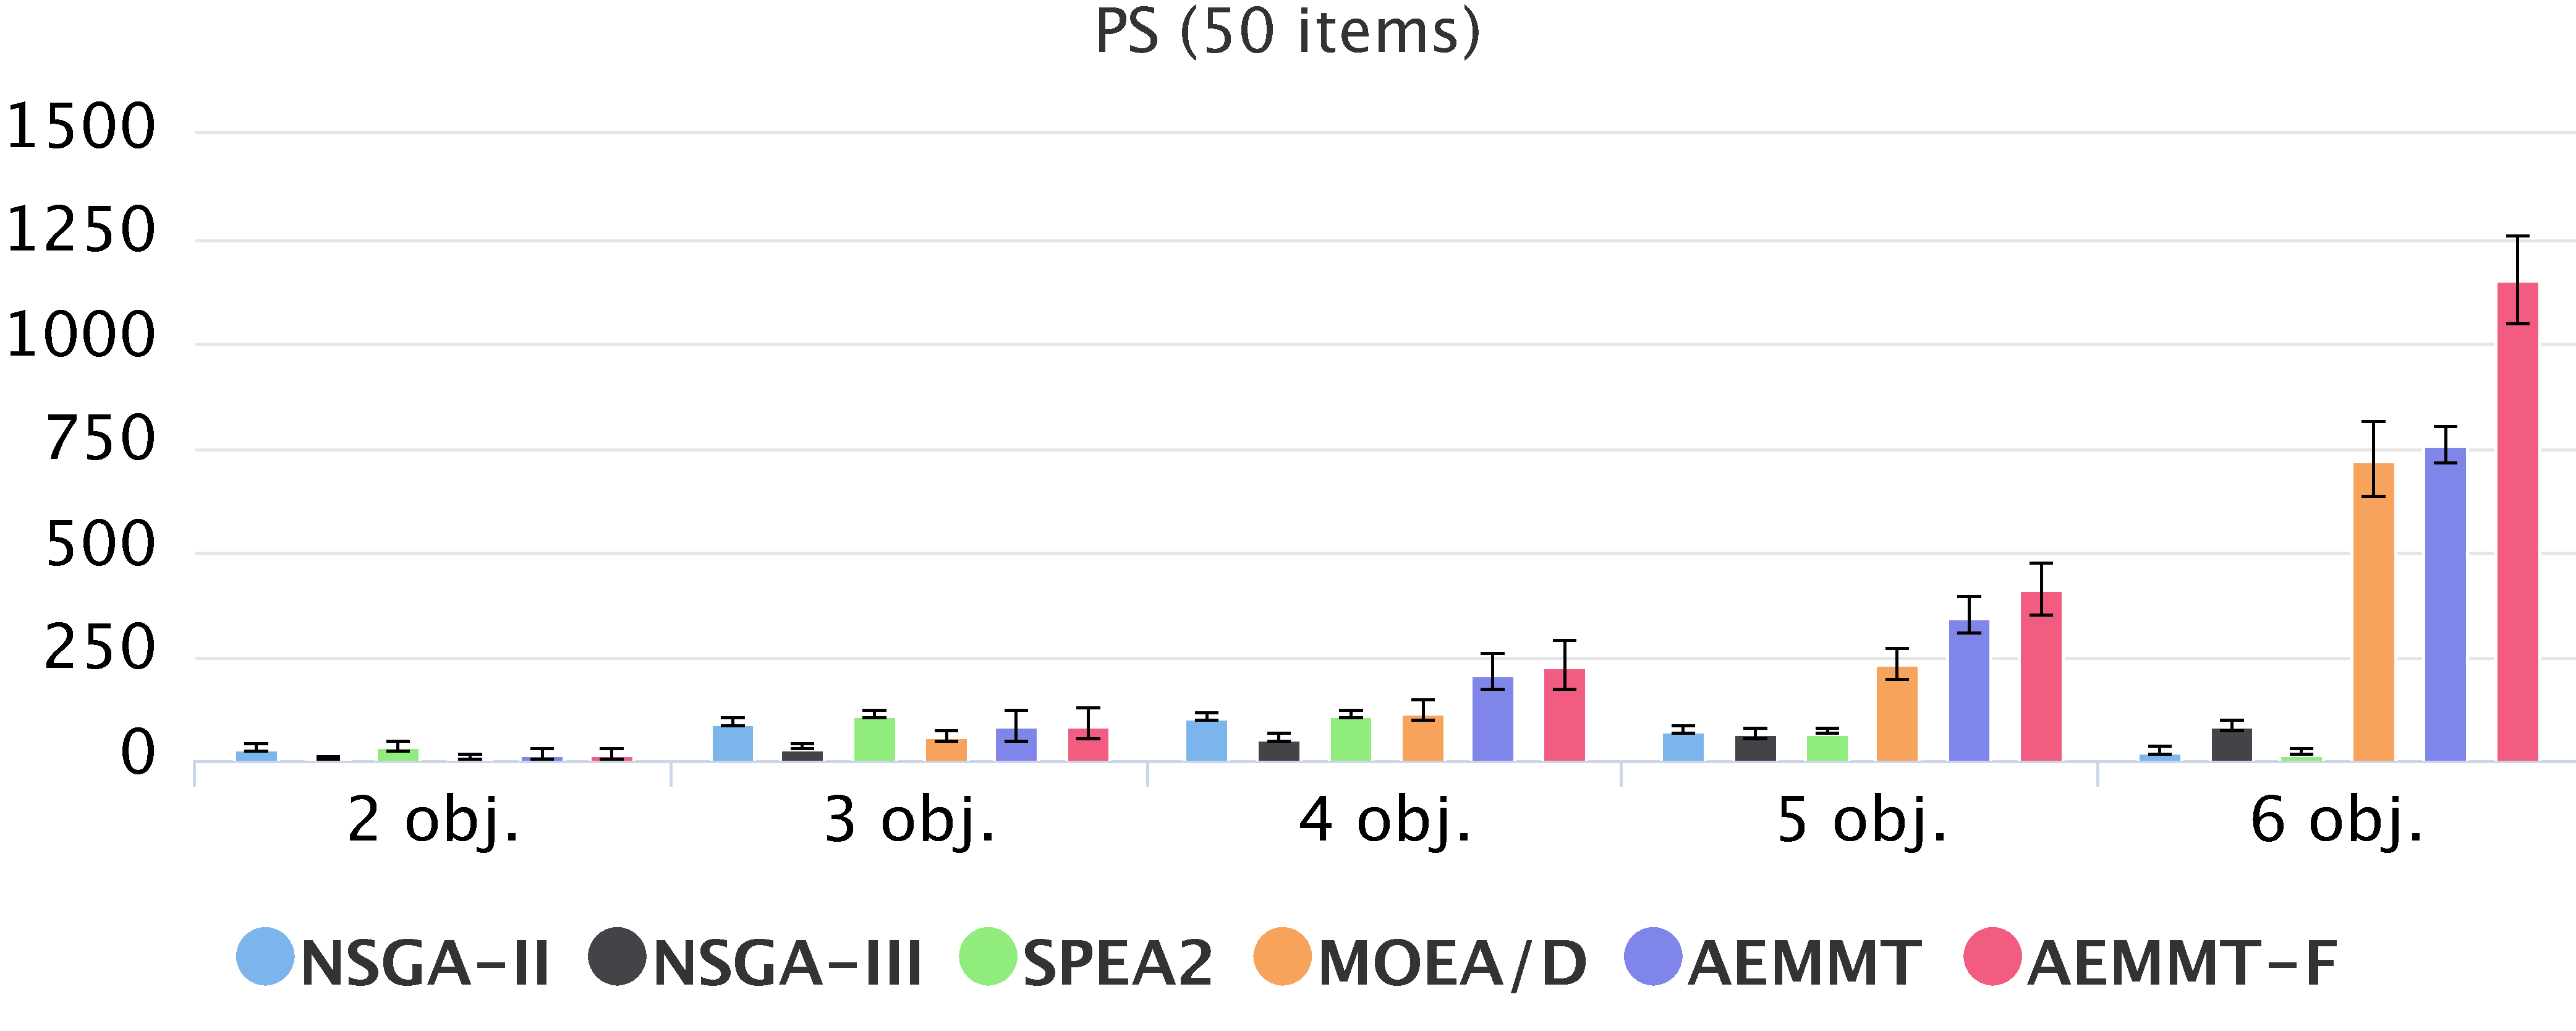
\includegraphics[width=1\textwidth]{cap_experimentos/figs/etapa1/ps-mkp-50}
\end{figure*}

O PMM com 50 itens (figura \ref{fig_exp1_mkp_50}) é um problema bem mais complexo que o PMM de 30 itens e já permite visualizar bem o comportamento de cada algoritmo nos diferentes cenários. Considerando as três métricas ($ER$, $GD$ e $PS$) os algoritmos clássicos (NSGA-II e SPEA2) são imbatíveis nas formulações com 2 e 3 objetivos. A partir de 4 objetivos a situação muda e o AEMMT passa a apresentar melhores resultados, ao aumentar os objetivos, o NSGA-II e o SPEA2 pioram enquanto o AEMMT mantém o $ER$ e o $GD$ estáveis enquanto melhora o $PS$. O MOEA/D é o segundo melhor algoritmo para problemas \textit{many-objectives} e o NSGA-III é o terceiro. Para o PMM de 50 itens, o AEMMT é claramente a melhor opção.

\begin{figure*}[!htbp]
	\caption{Etapa 1: resultados para o PMM com 100 itens}
	\label{fig_exp1_mkp_100}
	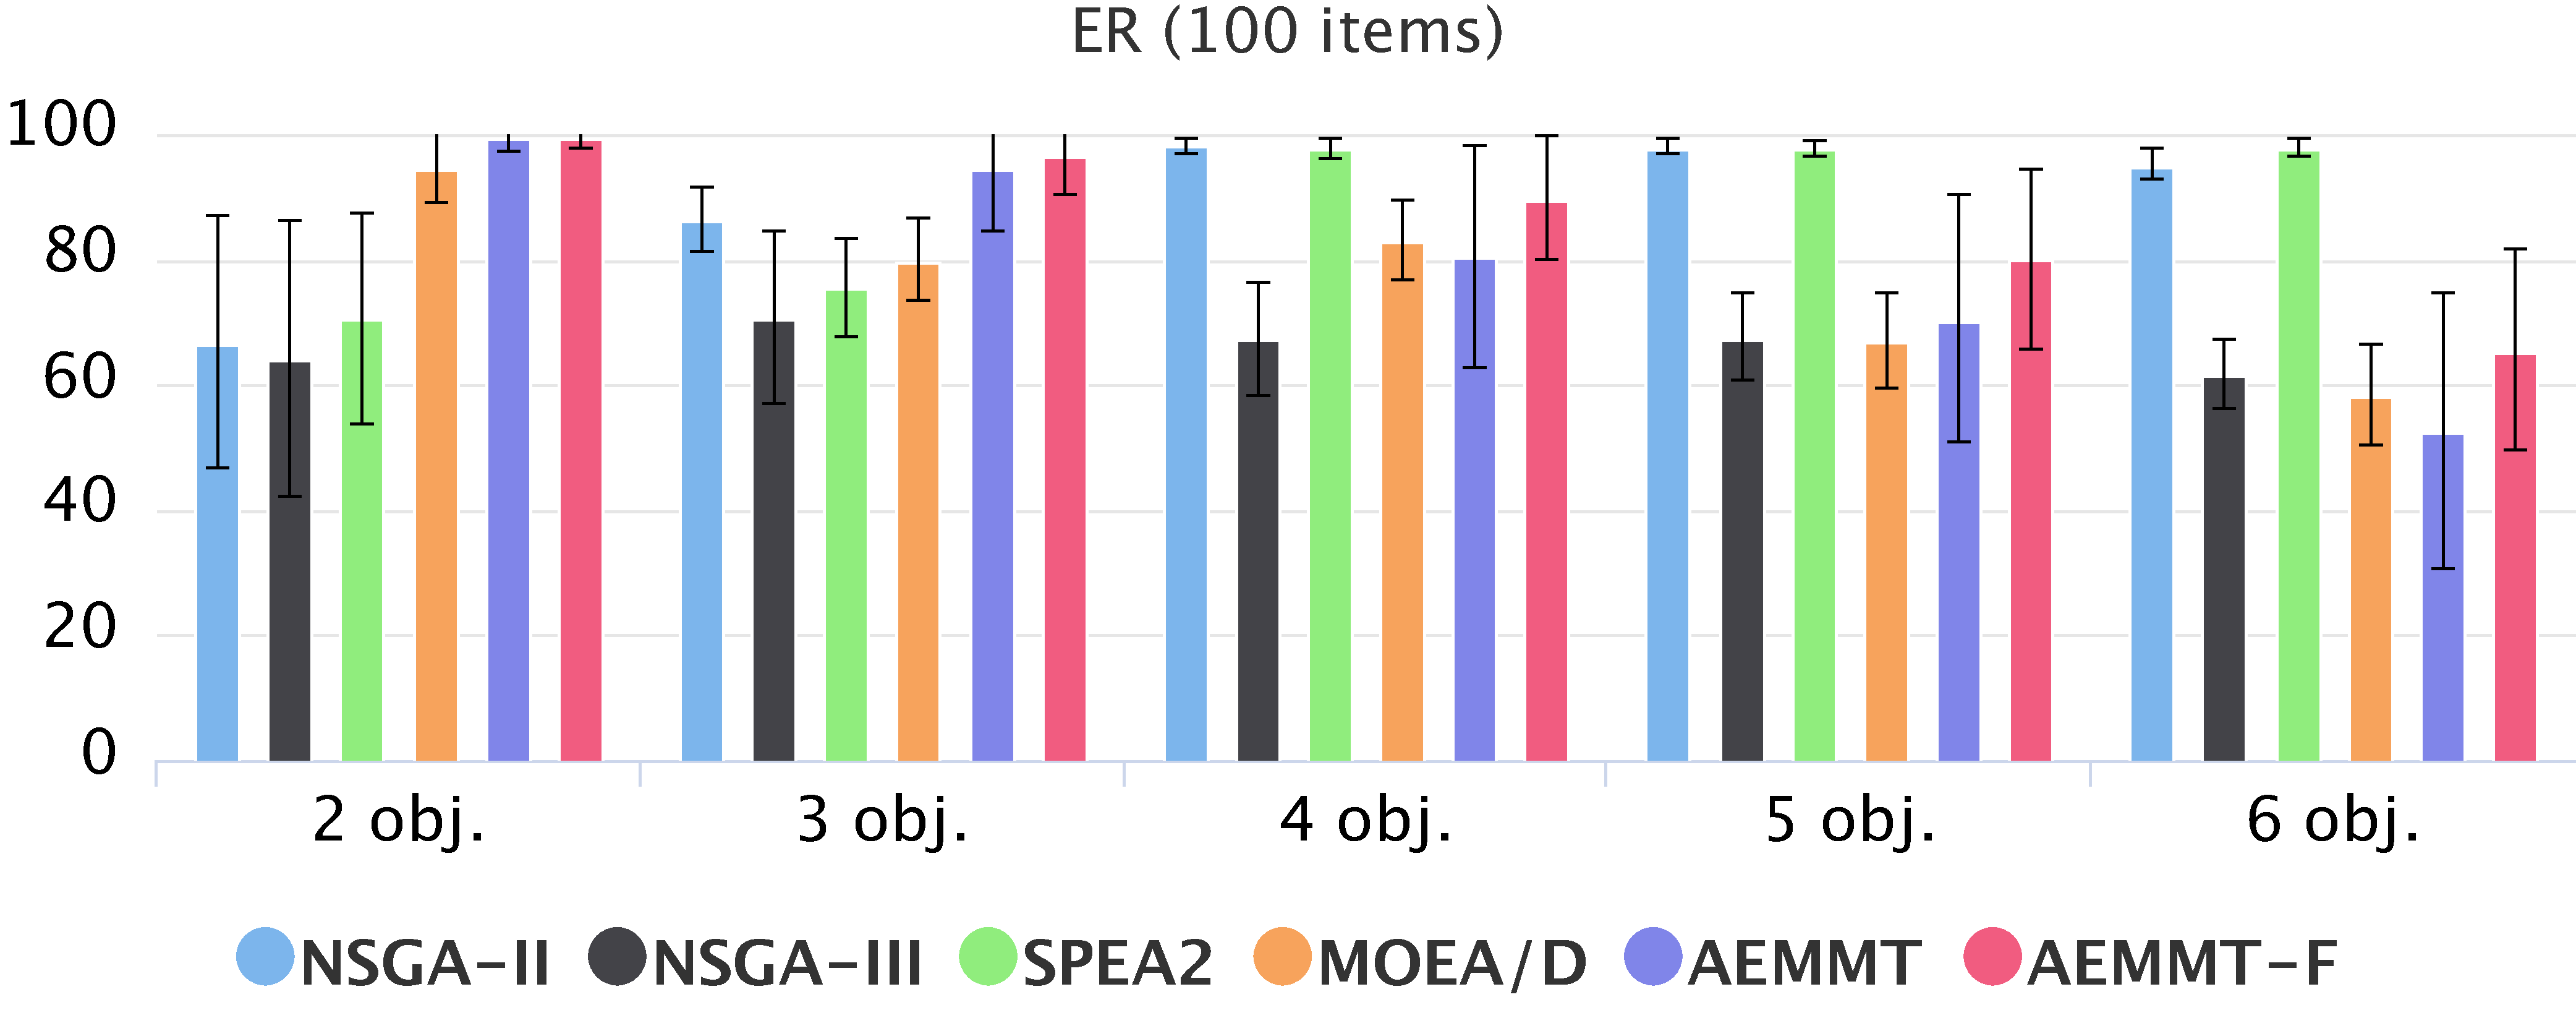
\includegraphics[width=1\textwidth]{cap_experimentos/figs/etapa1/er-mkp-100}
	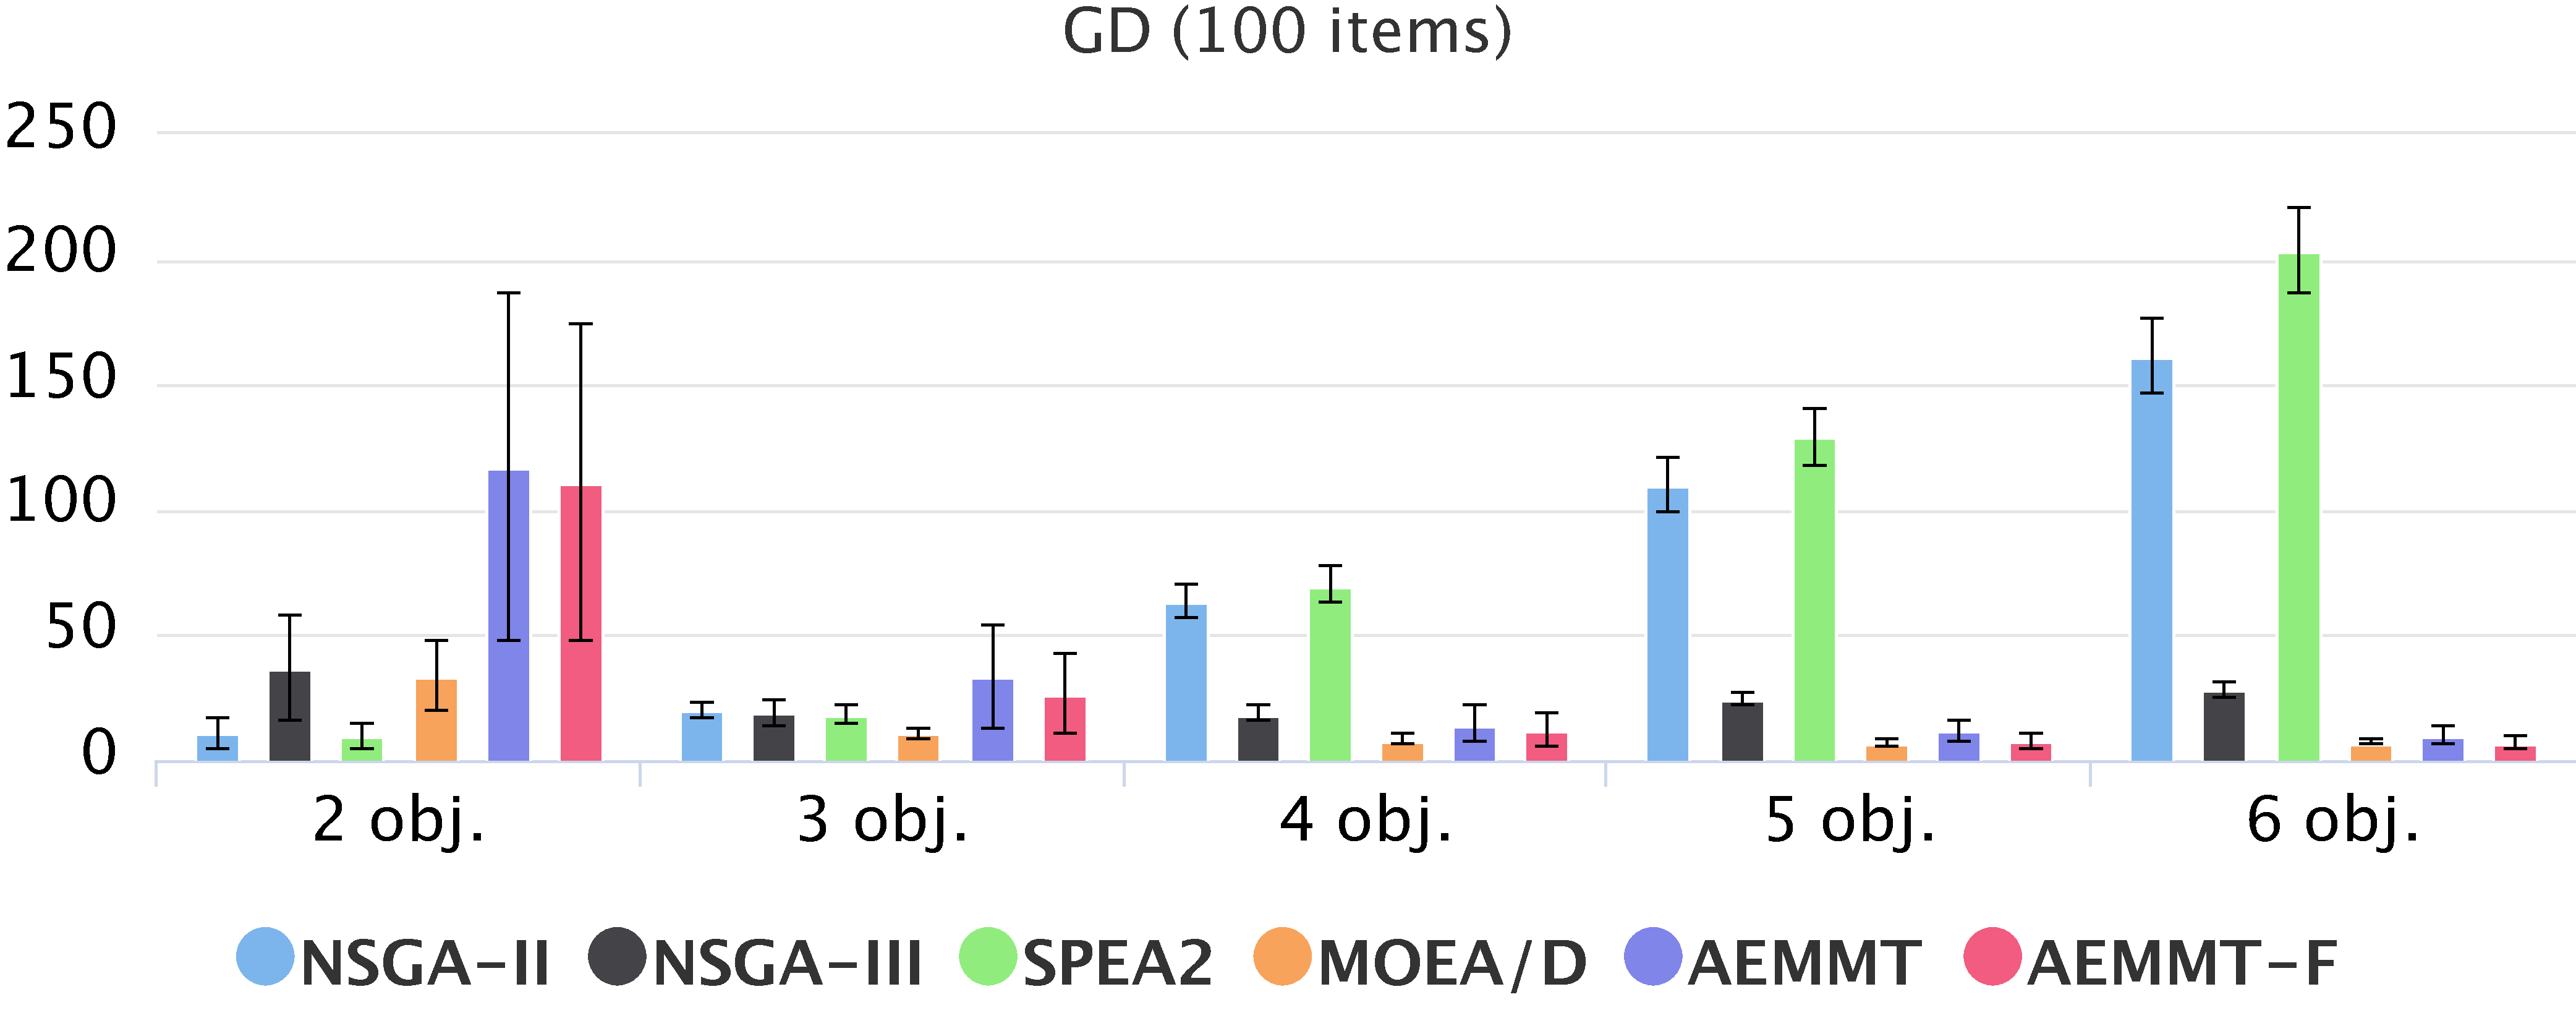
\includegraphics[width=1\textwidth]{cap_experimentos/figs/etapa1/gd-mkp-100}
	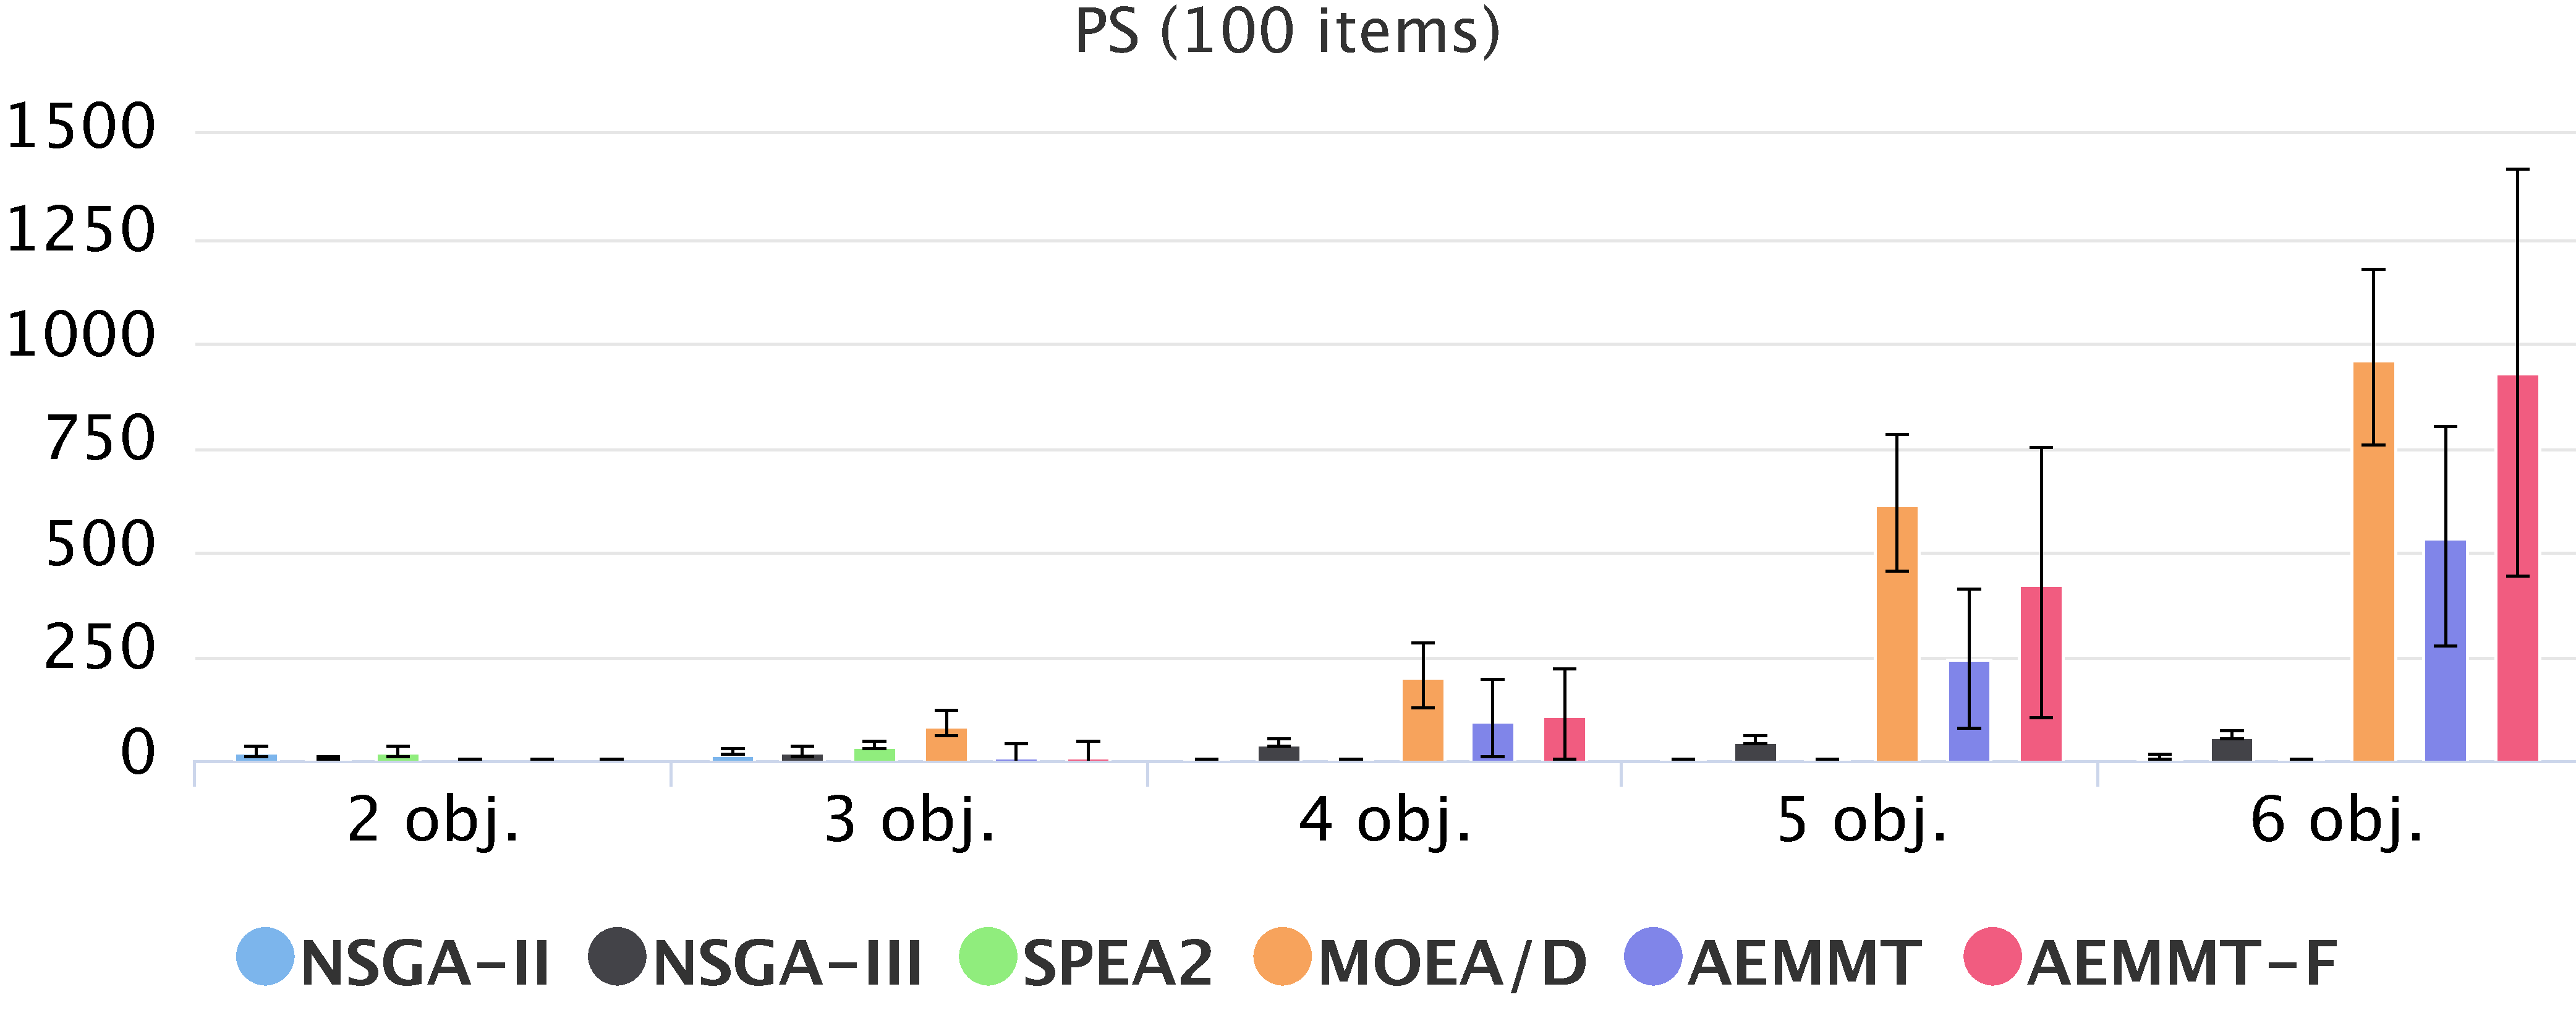
\includegraphics[width=1\textwidth]{cap_experimentos/figs/etapa1/ps-mkp-100}
\end{figure*}

O tamanho do espaço de busca no problema da mochila pode ser medido através da equação $2^n$, onde $n$ é o número de itens. Portanto, a complexidade do PMM com 100 itens (figura \ref{fig_exp1_mkp_100}) é absurdamente maior que os anteriores. Por essa razão, não foi possível encontrar um Pareto estável para as formulações de 4, 5 e 6 objetivos. Dessa forma, apesar de as métricas $ER$, $GD$ e $PS$ serem um bom indicativo da performance entre os algoritmos, a melhor forma de avaliação seria o hiper-volume. Um experimento parecido com este, mas utilizando o hiper-volume é apresentado na seção []. É difícil avaliar o problema de 100 itens, pois, já no erro é possível perceber que poucos algoritmos conseguiram encontrar boas soluções, a menor taxa de erro está acima de 50\%. No PMM de 100 itens o NSGA-III apresentou o menor $ER$ nos cenários de 2, 3, 4 e 5 objetivos, e na formulação de 6, foi ultrapassado pelos AEMMT e MOEA/D. Com relação ao $GD$, para 2 objetivos, o NSGA-II e o SPEA2 apresentaram os melhores resultados. Na formulação de 3 objetivos em diante o MOEA/D foi o algoritmo com menor $GD$, sendo que em 4, 5 e 6 objetivos o AEMMT obteve desempenho similar. A situação de repete ao analisar o $PS$, a partir de 3 objetivos, o MOEA/D traz um conjunto maior de soluções na fronteira de Pareto, seguido pelo AEMMT a partir de 4 objetivos.

\begin{figure*}[!htbp]
	\caption{Etapa 1: resultados agrupados para o PMM com 30, 50 e 100 itens}
	\label{fig_exp1_mkp_todos}
	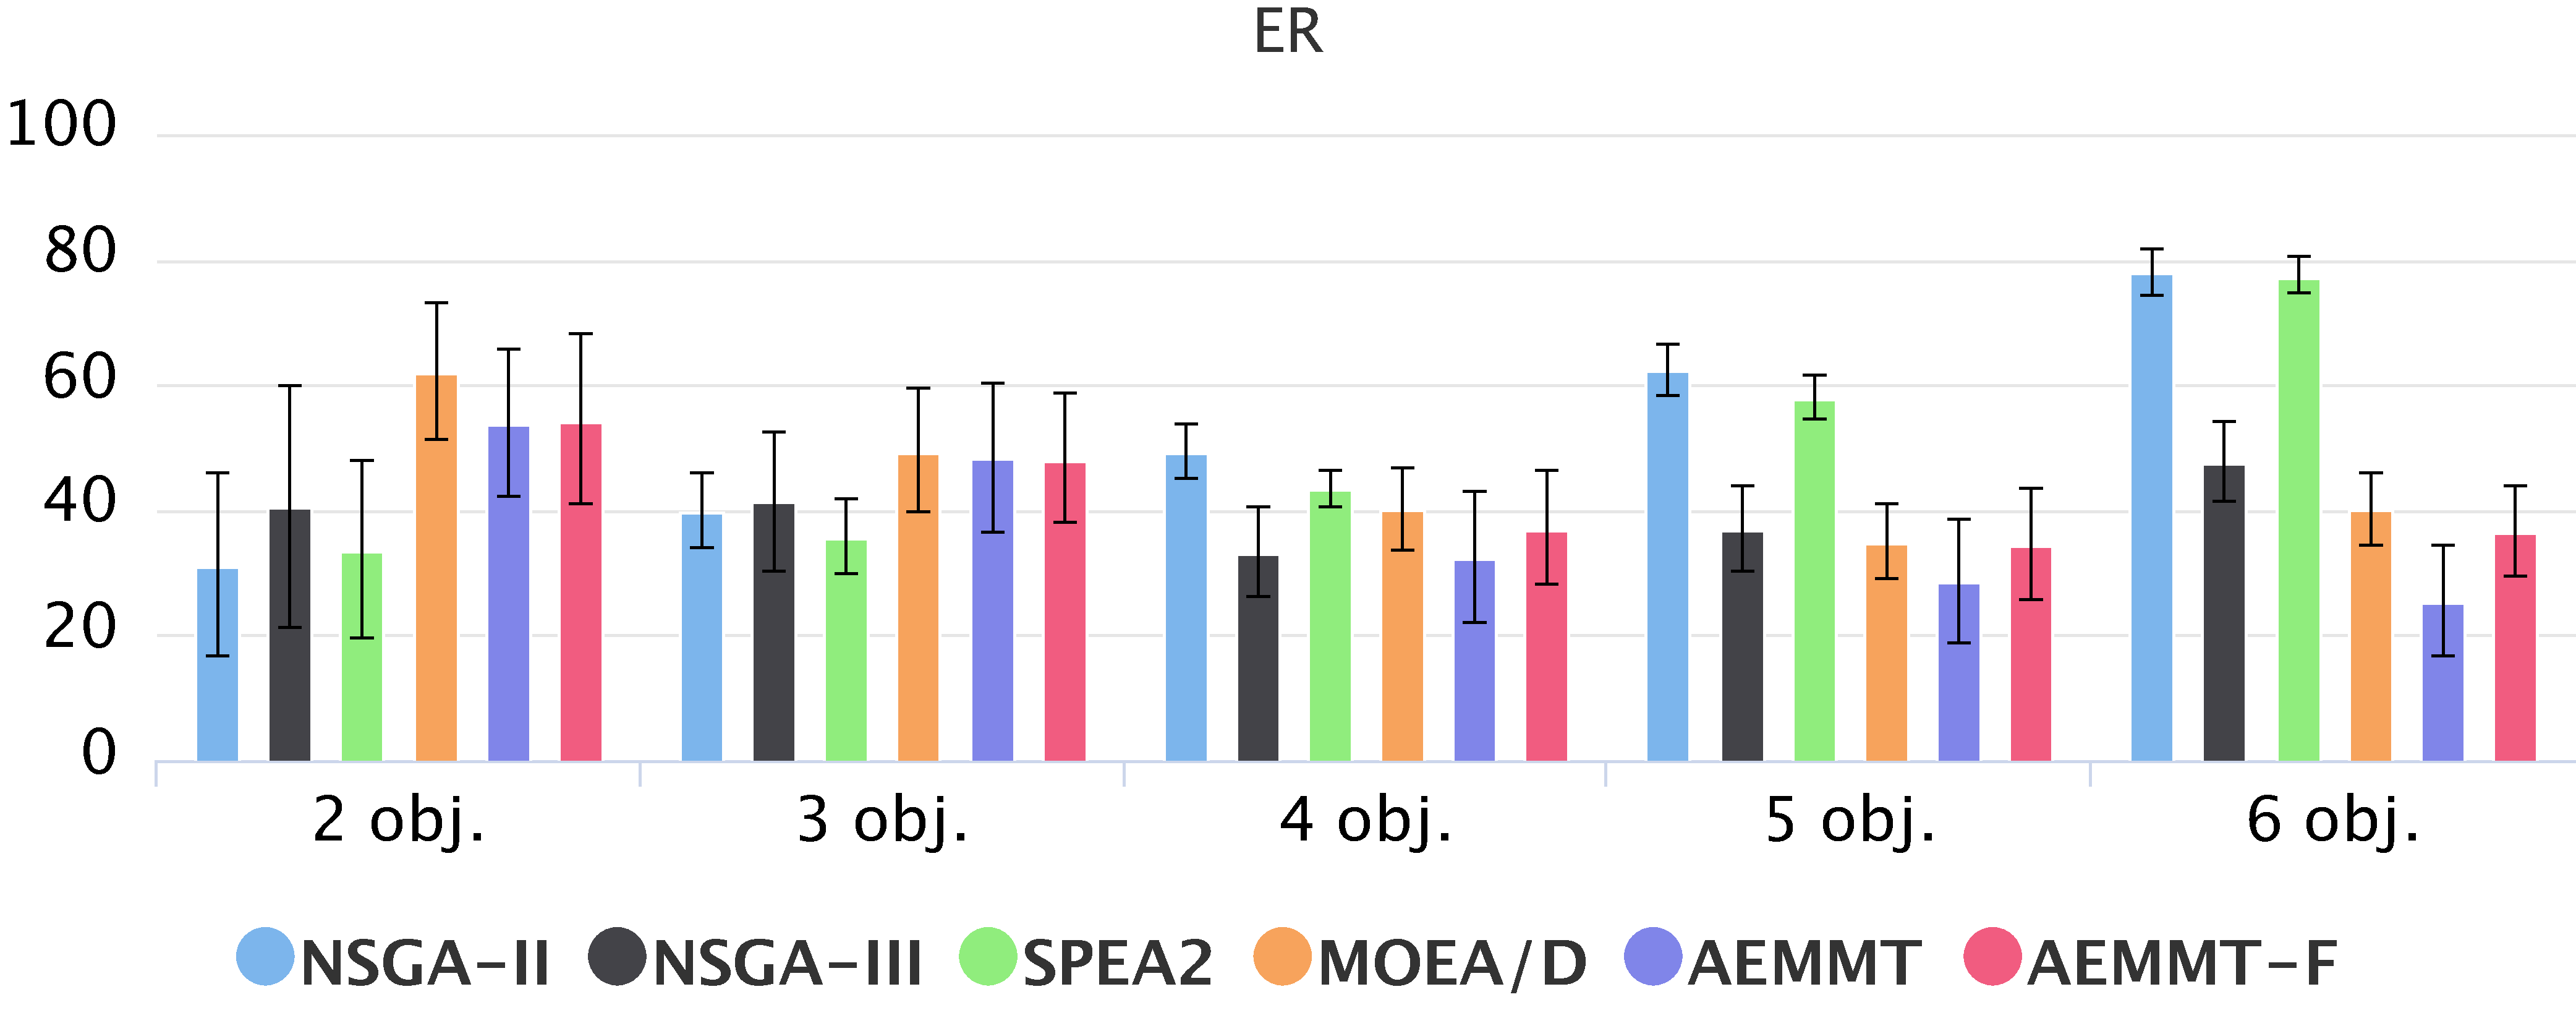
\includegraphics[width=1\textwidth]{cap_experimentos/figs/etapa1/er-mkp-todos}
	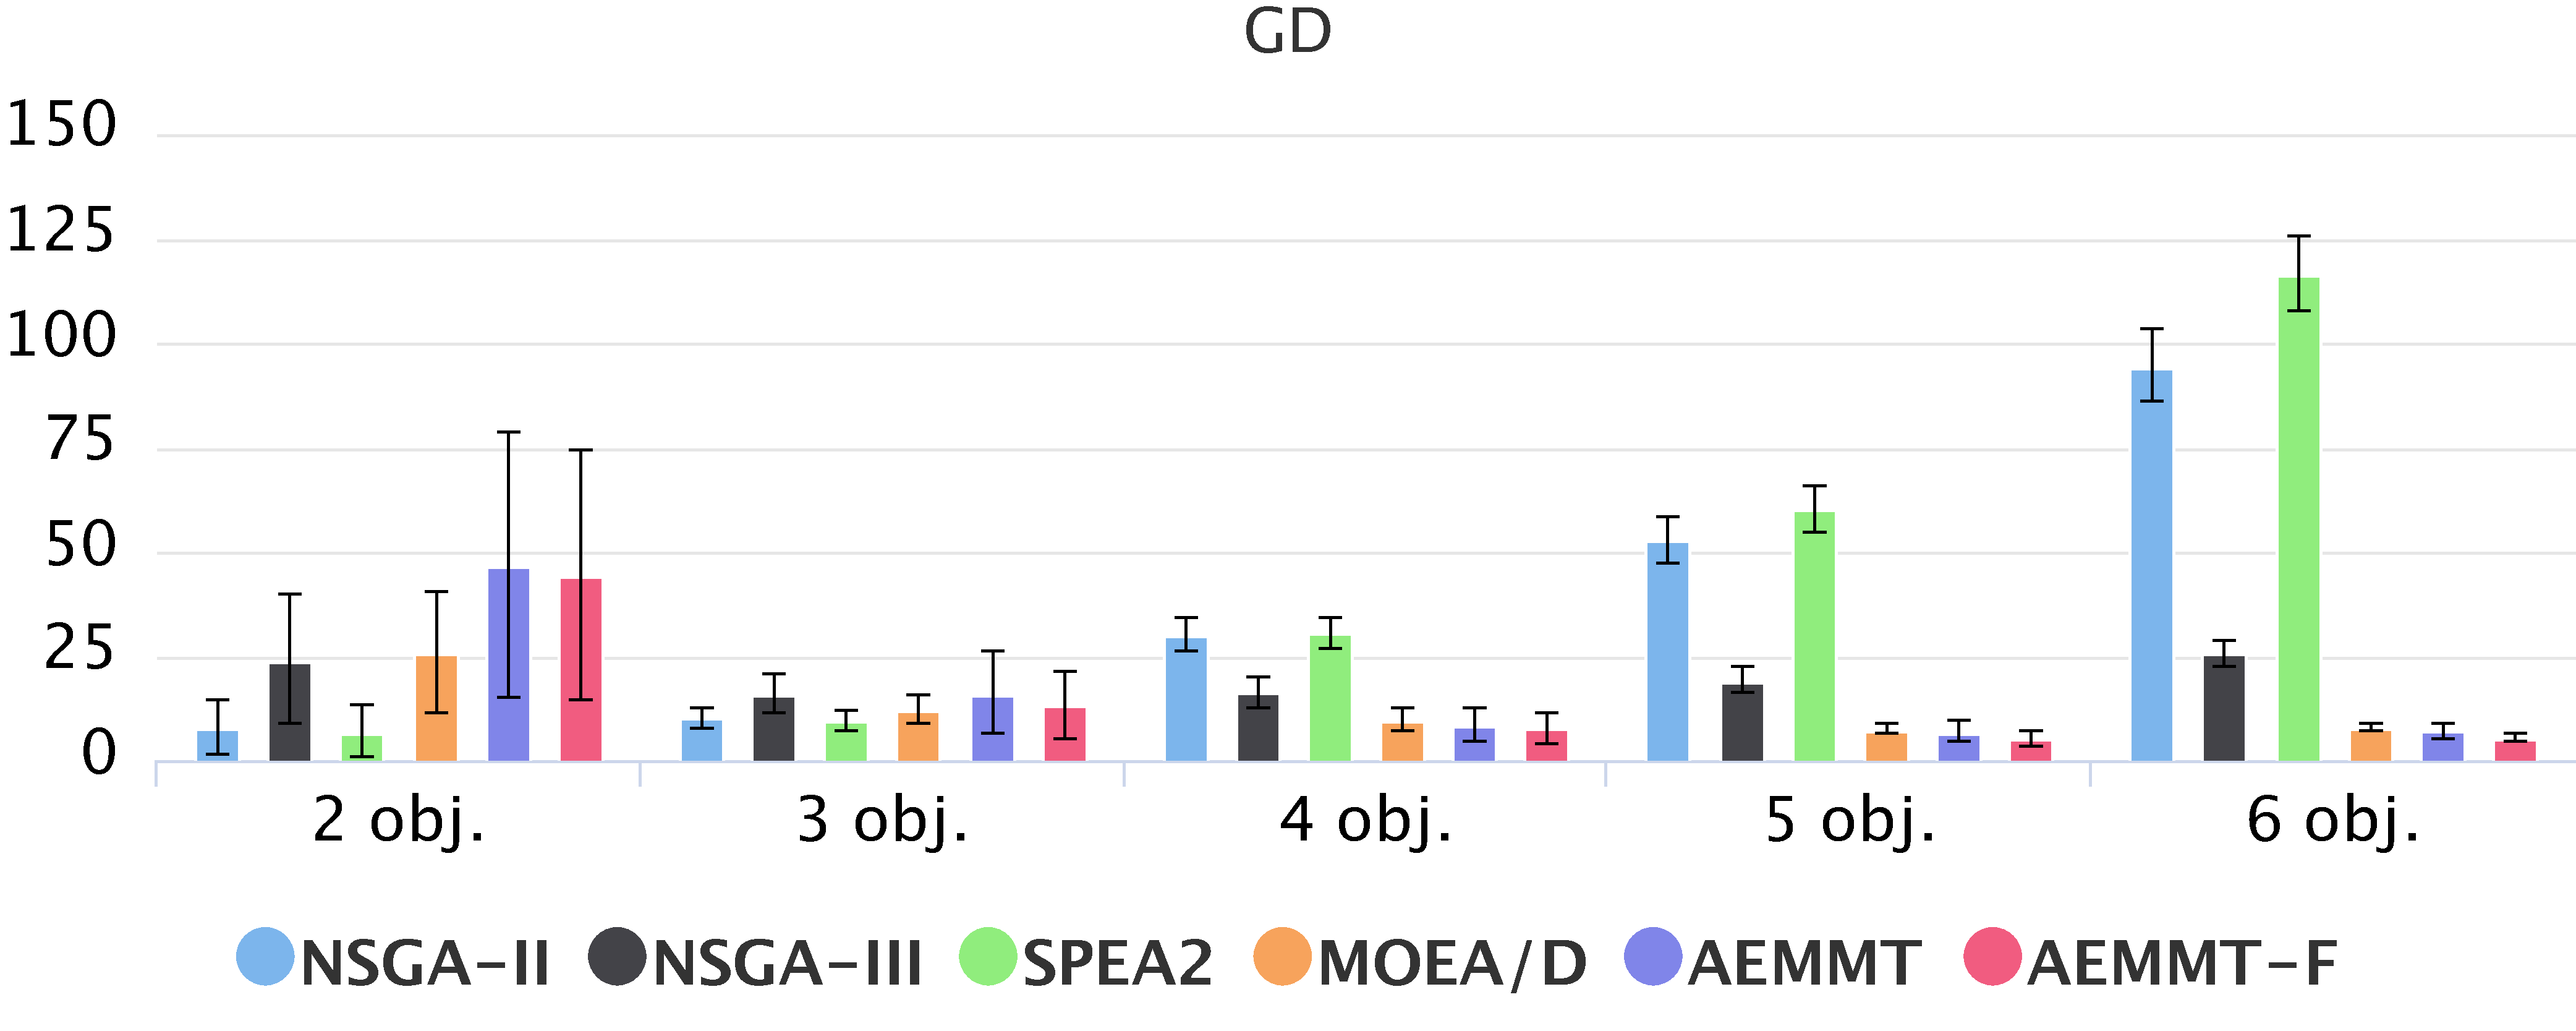
\includegraphics[width=1\textwidth]{cap_experimentos/figs/etapa1/gd-mkp-todos}
	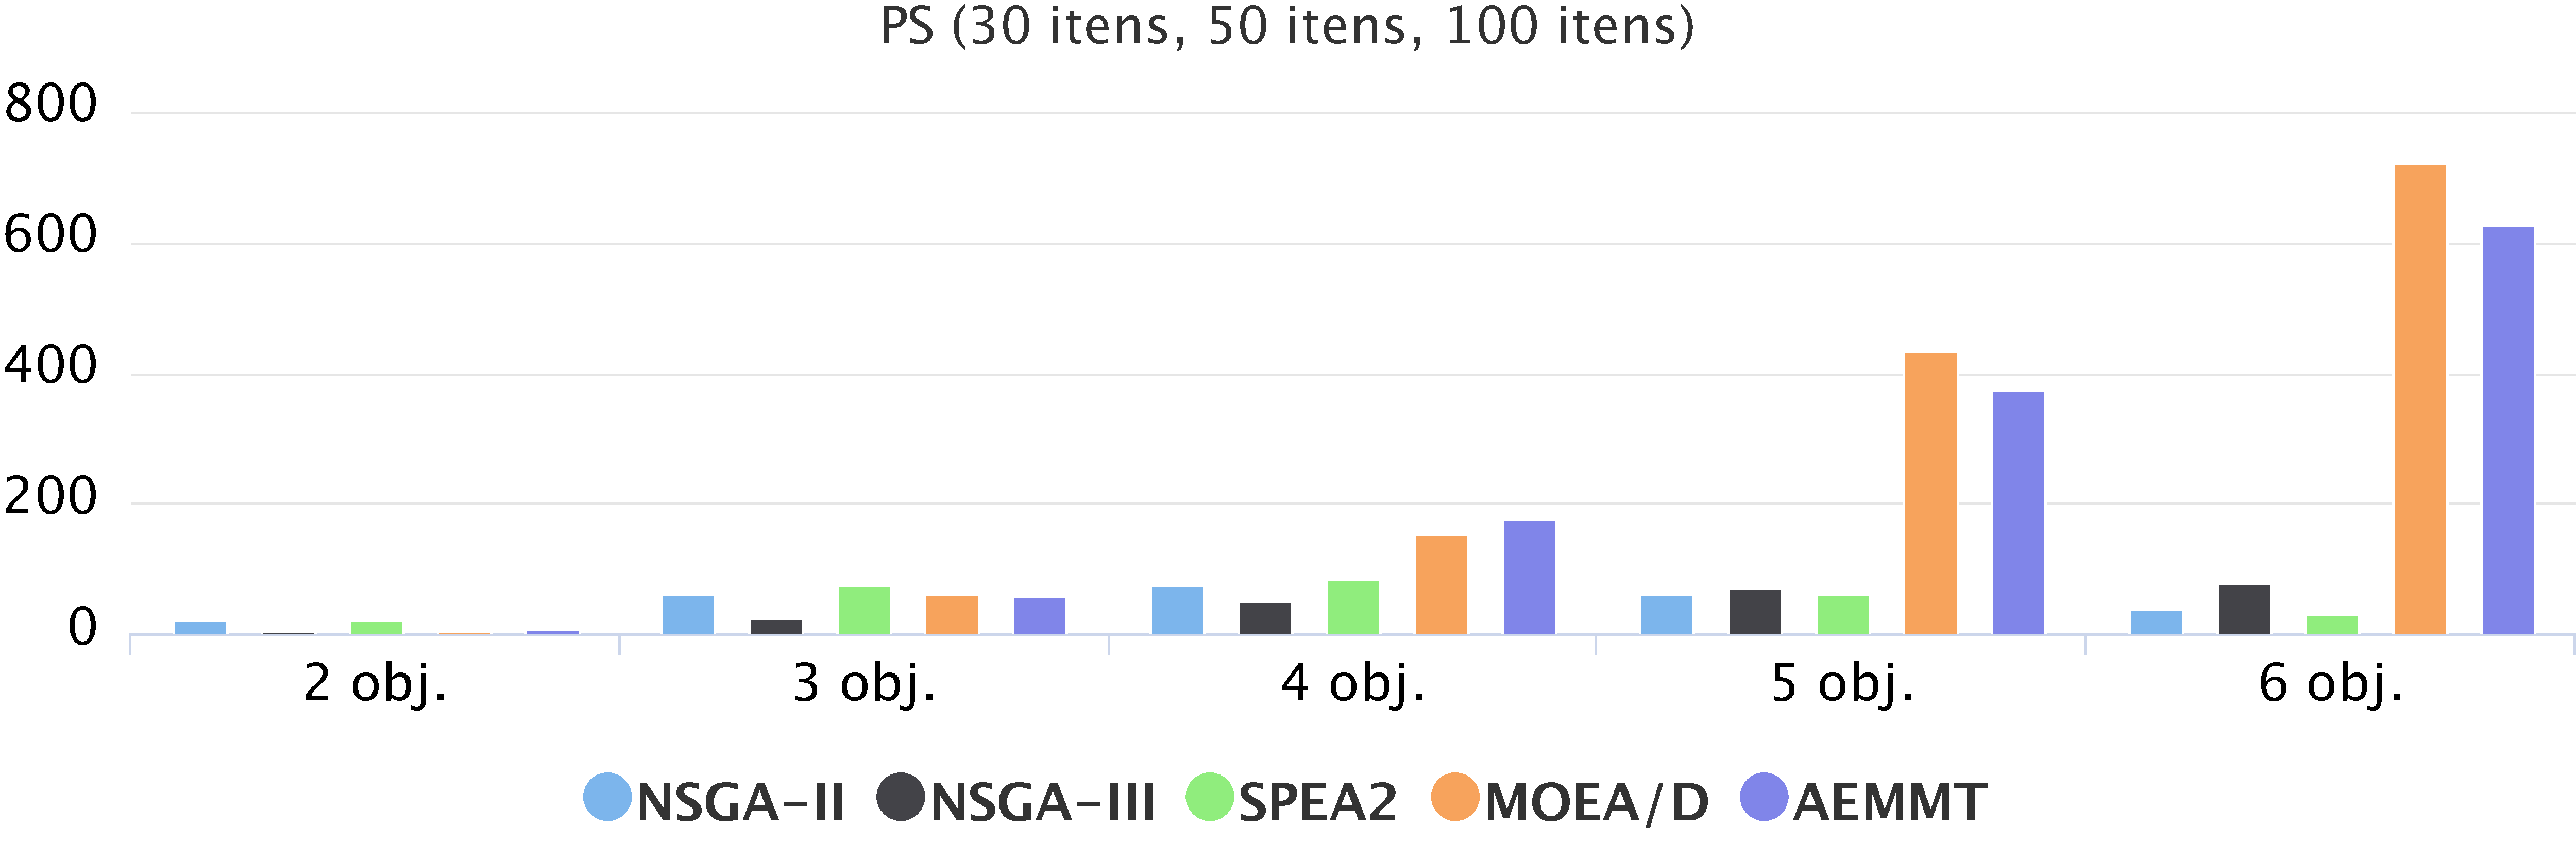
\includegraphics[width=1\textwidth]{cap_experimentos/figs/etapa1/ps-mkp-todos}
\end{figure*}

A figura \ref{fig_exp1_mkp_100} apresenta os resultados do PMM de 30, 50 e 100 itens de forma condensada para que se possa ver, de forma geral, o comportamento dos algoritmos nas diferentes formulações de objetivo. Os gráficos representam as médias entre os três cenários de dificuldade (30, 50 e 100 itens). Como esperado, considerando a literatura correlata, o NSGA-II e o SPEA2 são os melhores algoritmos para as formulações de 2 e 3 objetivos, apresentam melhor $ER$, $GD$ e $PS$. Por outro lado, a partir de 4 objetivos, o desempenho de ambos os algoritmos cai consideravelmente, enquanto o AEMMT assume a liderança. O NSGA-III, no problema de 4 objetivos, apresenta um erro quase tão baixo quento o AEMMT, mas seu $GD$ e $PS$ são piores. o MOEA/D, para 5 e 6 objetivos, apresenta o segundo melhor resultado em qualquer uma das métricas. Em resumo, o NSGA-III não parece uma boa opção em nenhum dos casos, pois sempre há outro algoritmo que obtém um melhor resultado. O NSGA-II e o SPEA2 são igualmente bons e os melhores em problemas com poucos objetivos. O AEMMT e o MOEA/D são ótimas opções para problemas a partir de 4 objetivos, sendo que o MOEA/D confere um melhor $PS$ enquanto o AEMMT providencia menor taxa de erro.

\begin{figure*}[!htbp]
	\caption{Etapa 1: resultados para o PRM na rede $R_1$}
	\label{fig_exp1_mrp_r1}
	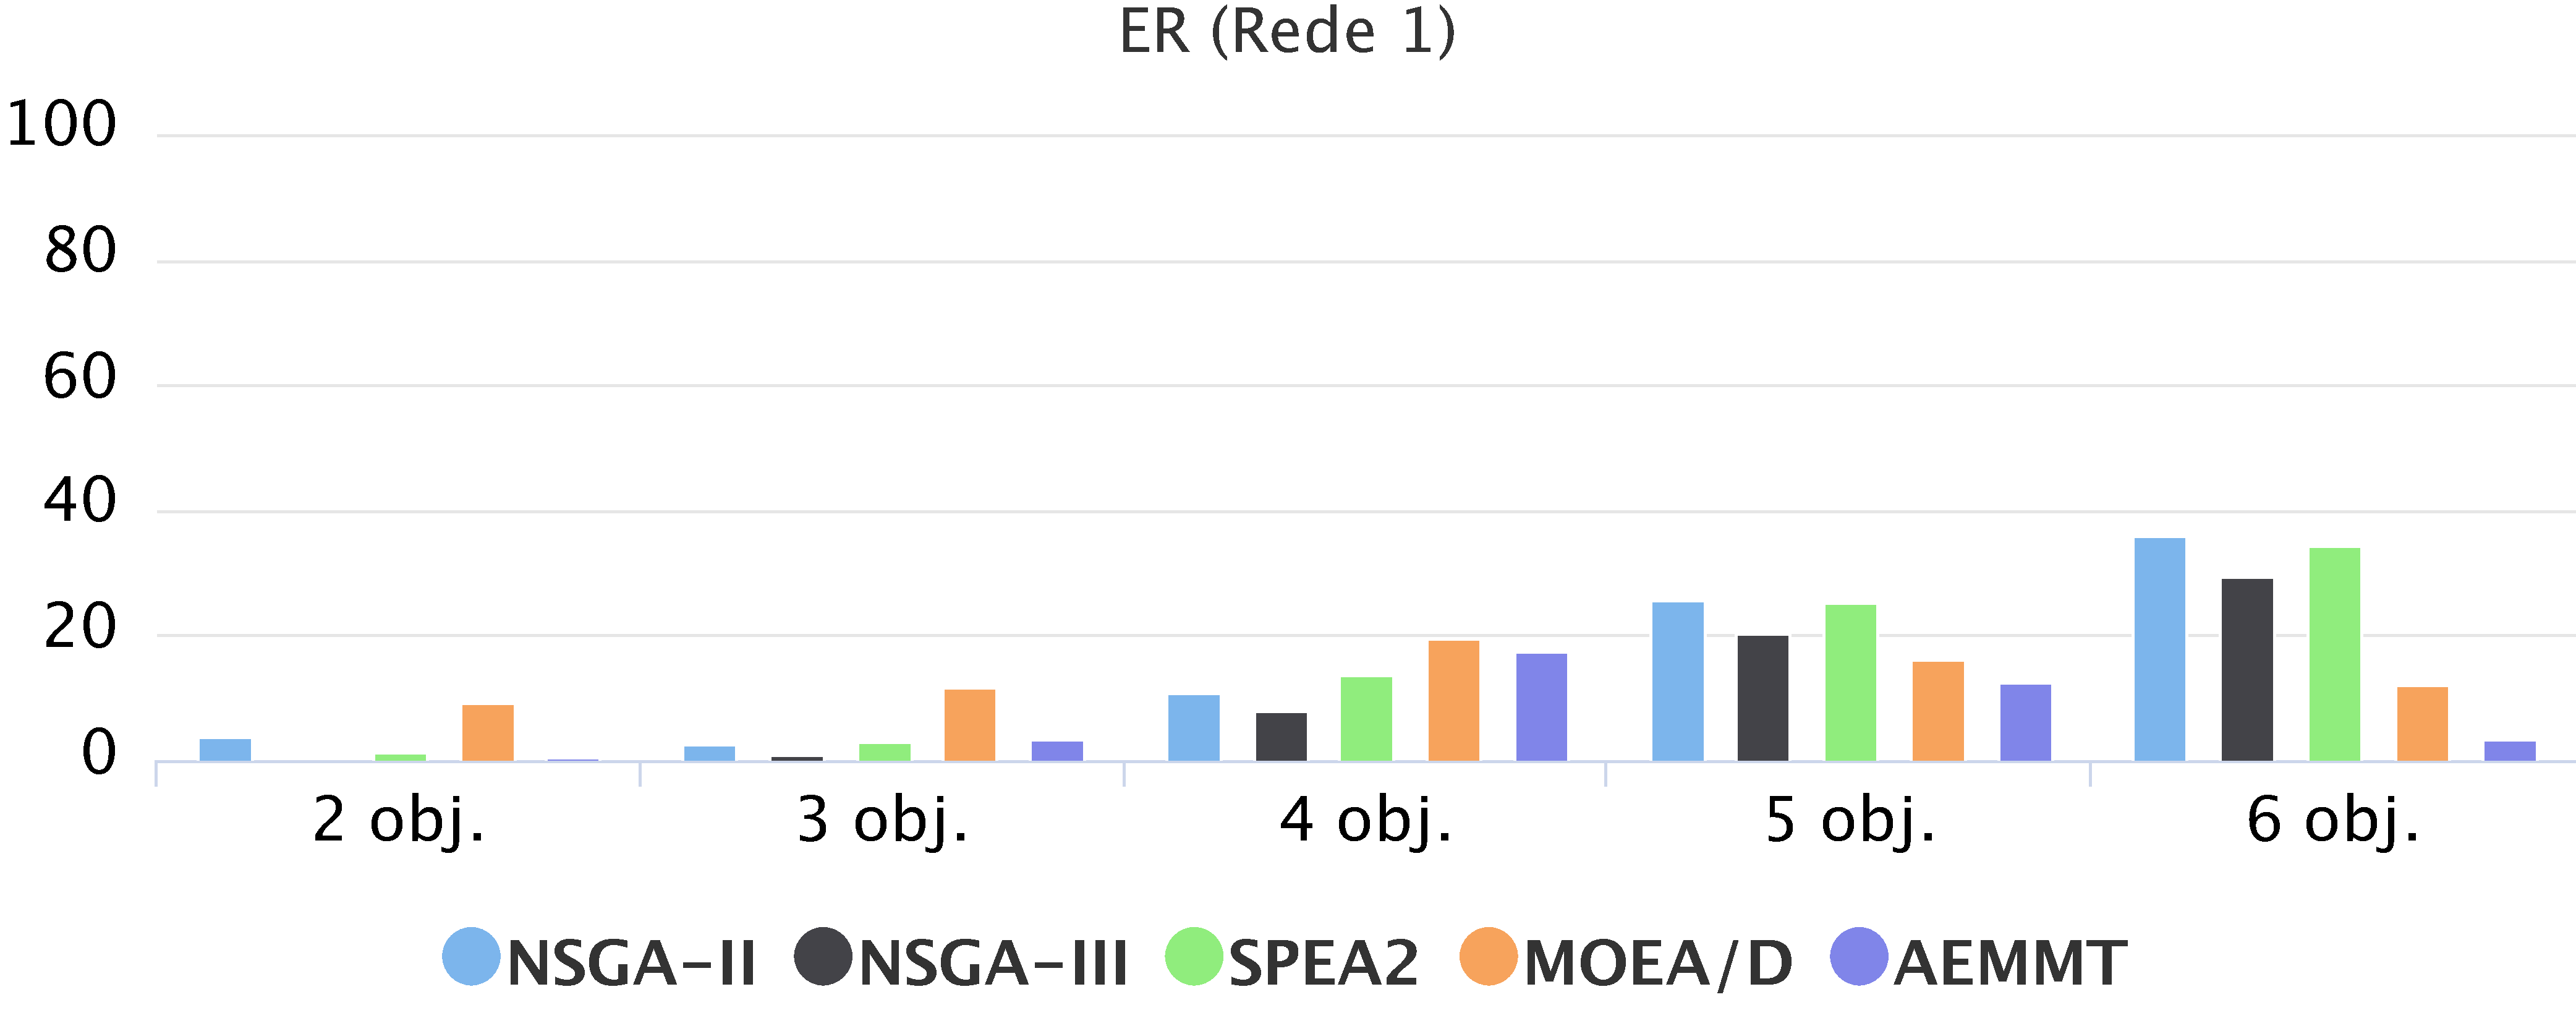
\includegraphics[width=1\textwidth]{cap_experimentos/figs/etapa1/er-mrp-r1}
	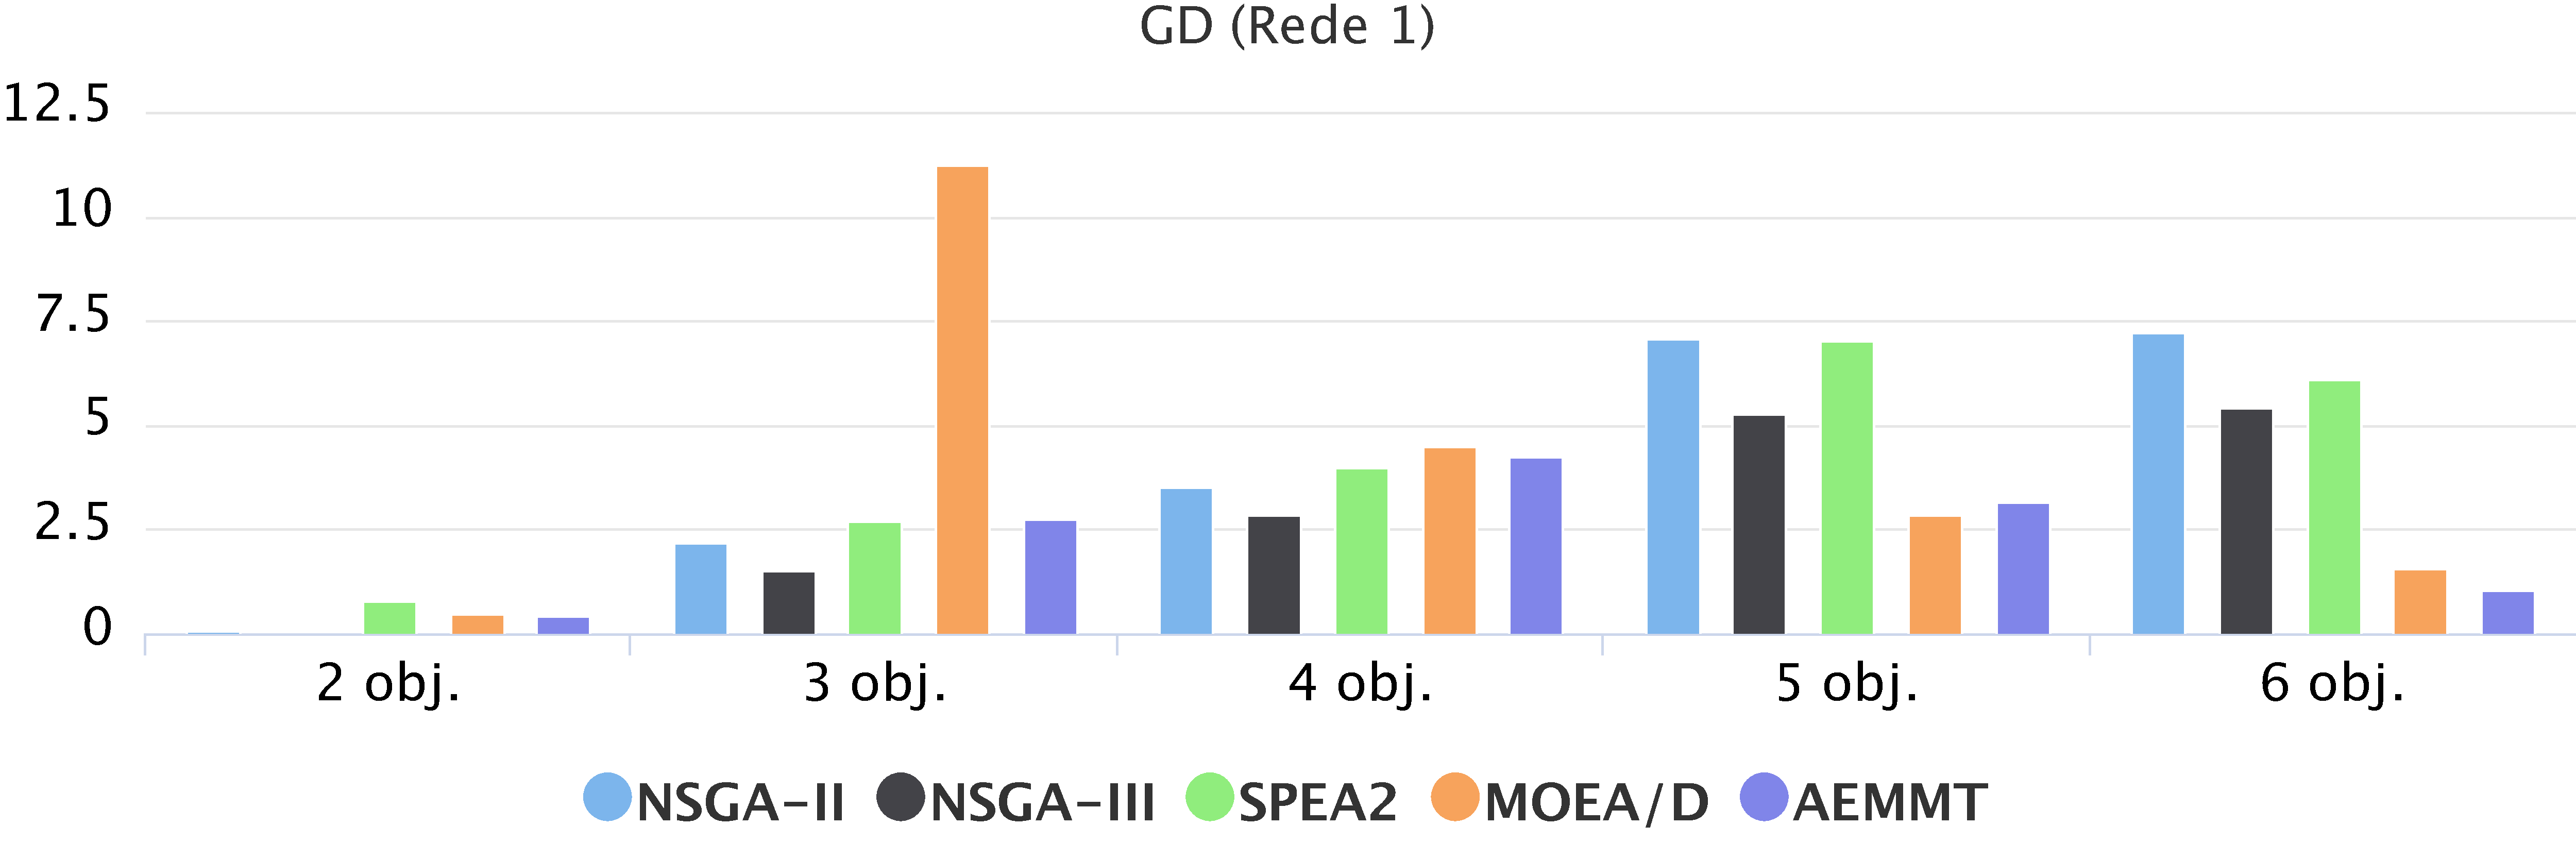
\includegraphics[width=1\textwidth]{cap_experimentos/figs/etapa1/gd-mrp-r1}
	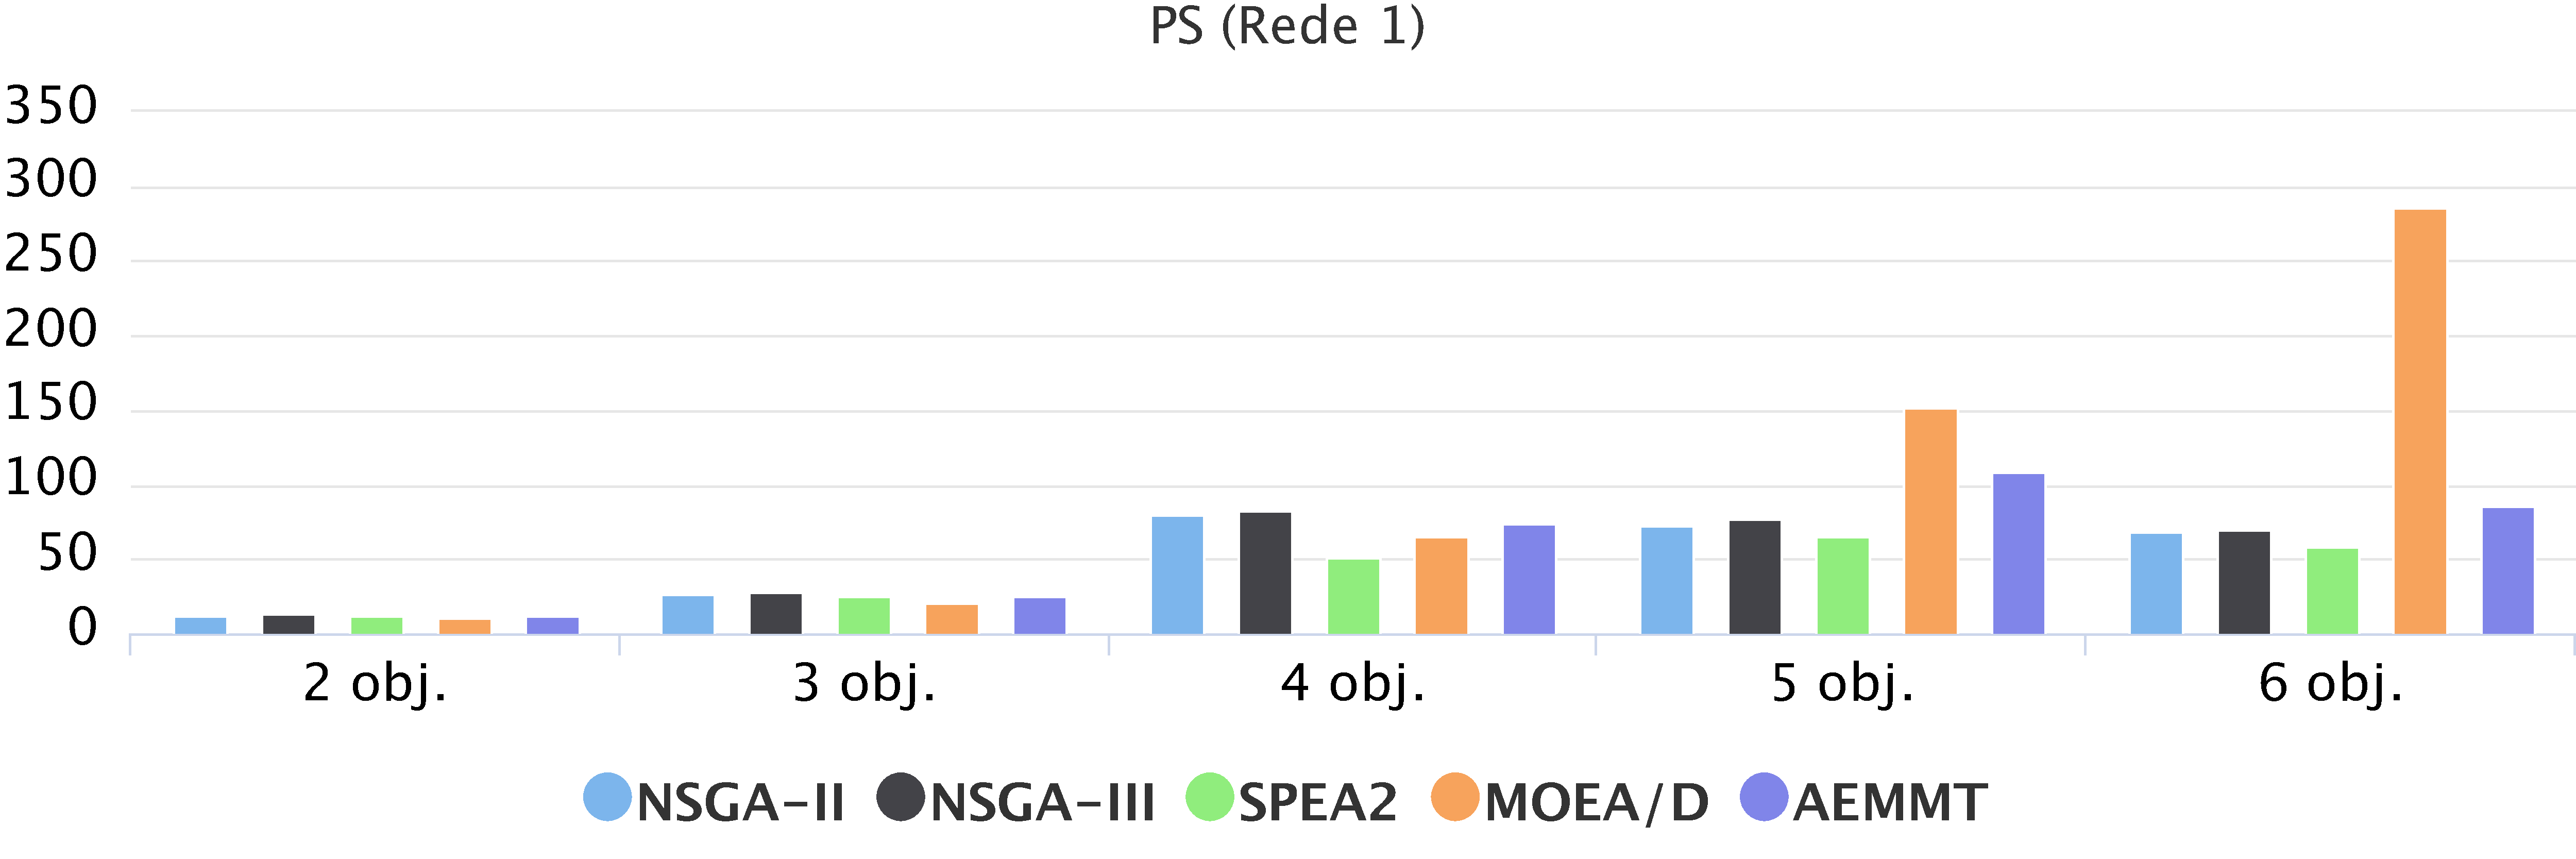
\includegraphics[width=1\textwidth]{cap_experimentos/figs/etapa1/ps-mrp-r1}
\end{figure*}

O PRM sobre a rede 1 (figura \ref{fig_exp1_mrp_r1}), a mais simples dentre elas, mostrou bons resultados para todos os algoritmos. Diferente do esperado, o NSGA-III mostrou o melhor resultado ($ER$, $GD$ e $PS$) para os problemas com 2, 3 e 4 objetivos. A partir de 5 objetivos, o AEMMT e o MOEA/D são os dois melhores métodos, o primeiro apresenta uma menor taxa de erro, enquanto o segundo obtém um Pareto de maior cardinalidade. Para poucos objetivos, o NSGA-III é claramente o melhor método, para 5 ou mais critérios de otimização, ambos AEMMT e MOEA/D são boas opções.

\begin{figure*}[!htbp]
	\caption{Etapa 1: resultados para o PRM na rede $R_2$}
	\label{fig_exp1_mrp_r2}
	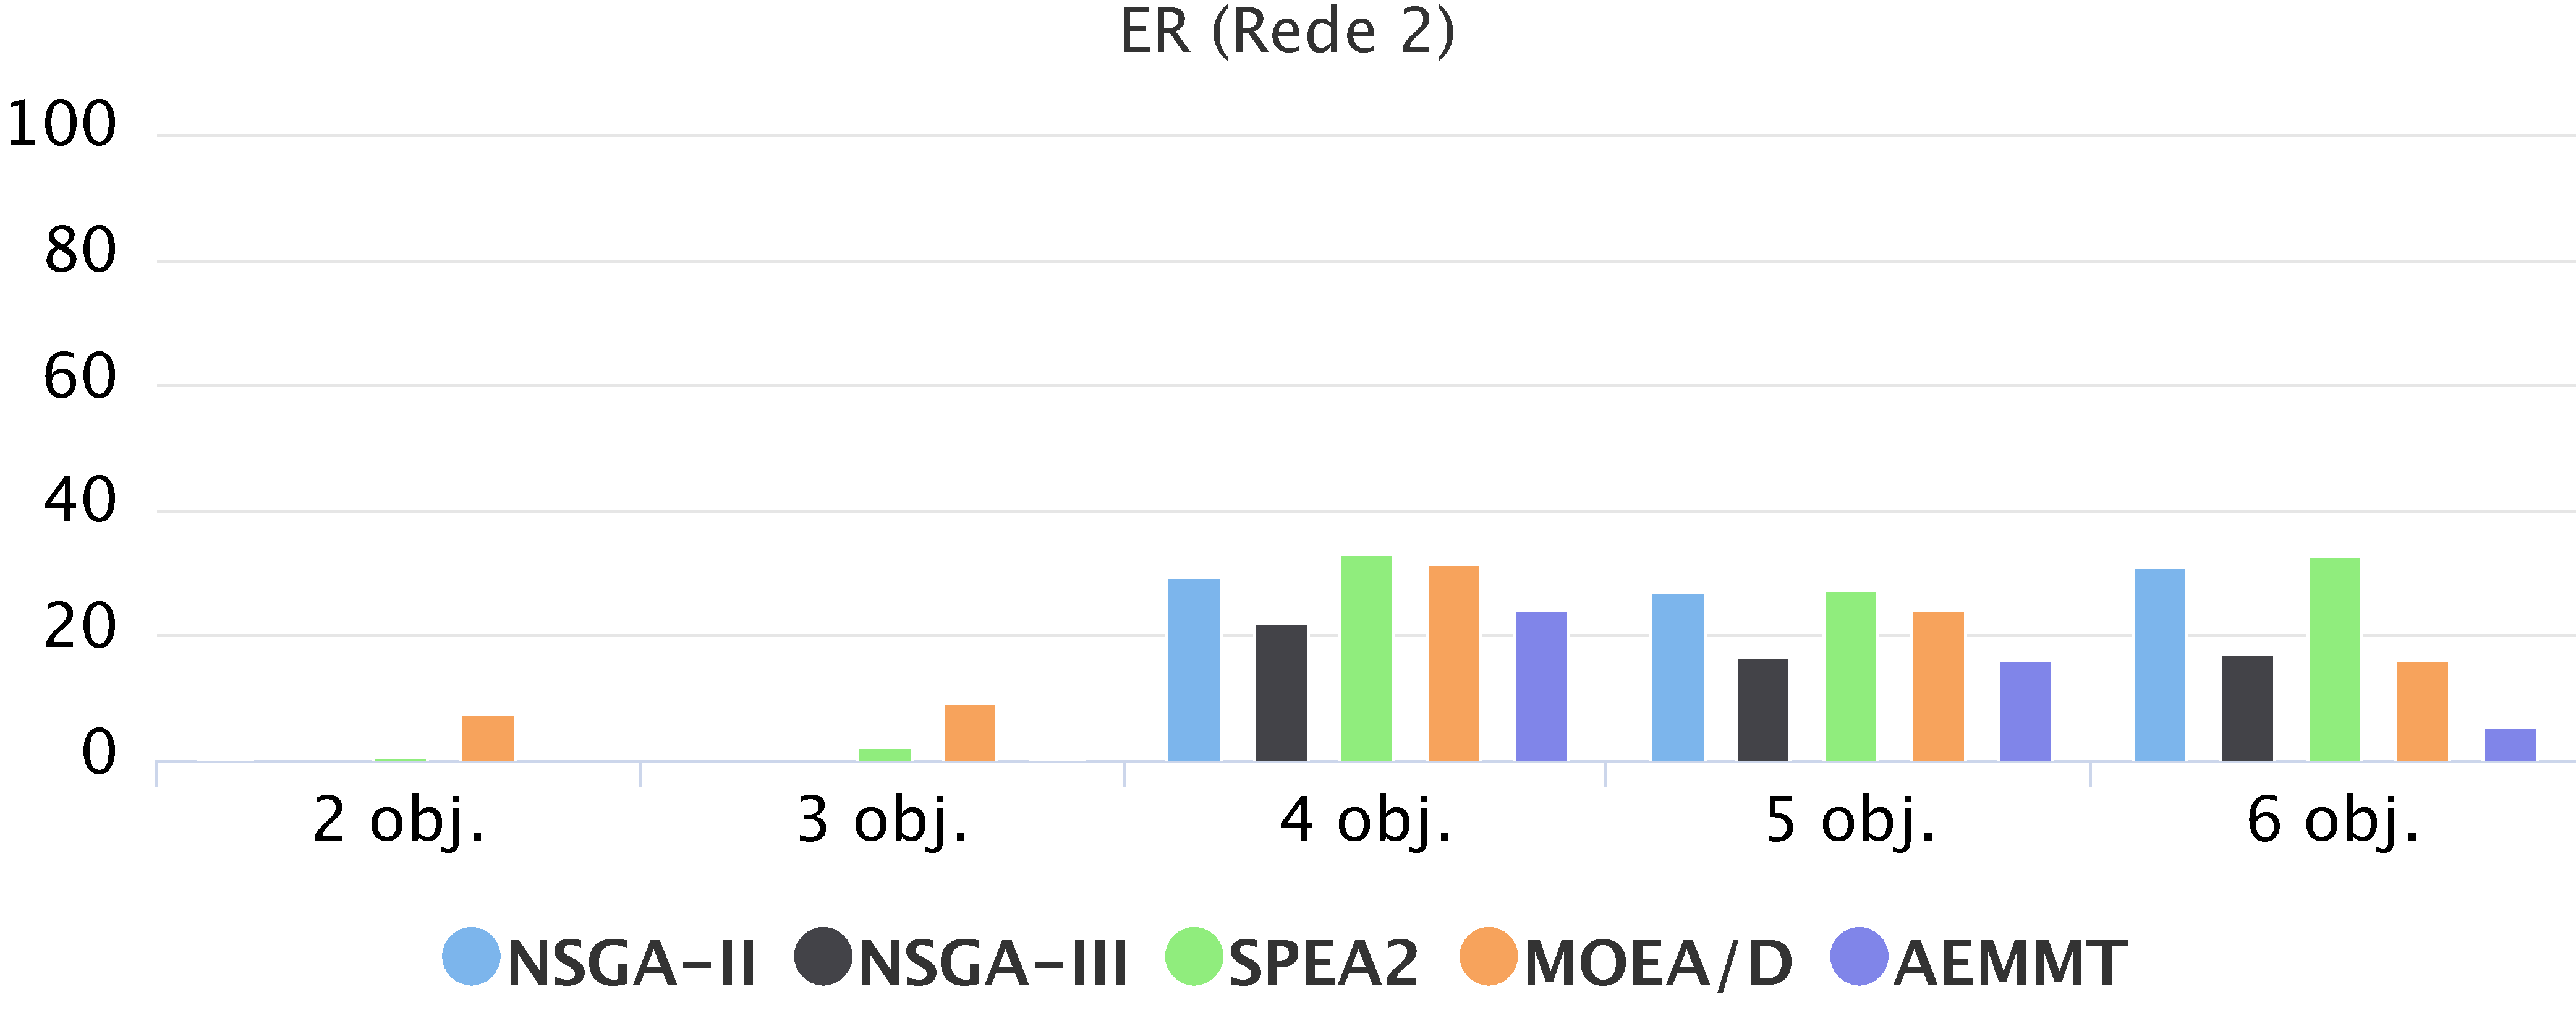
\includegraphics[width=1\textwidth]{cap_experimentos/figs/etapa1/er-mrp-r2}
	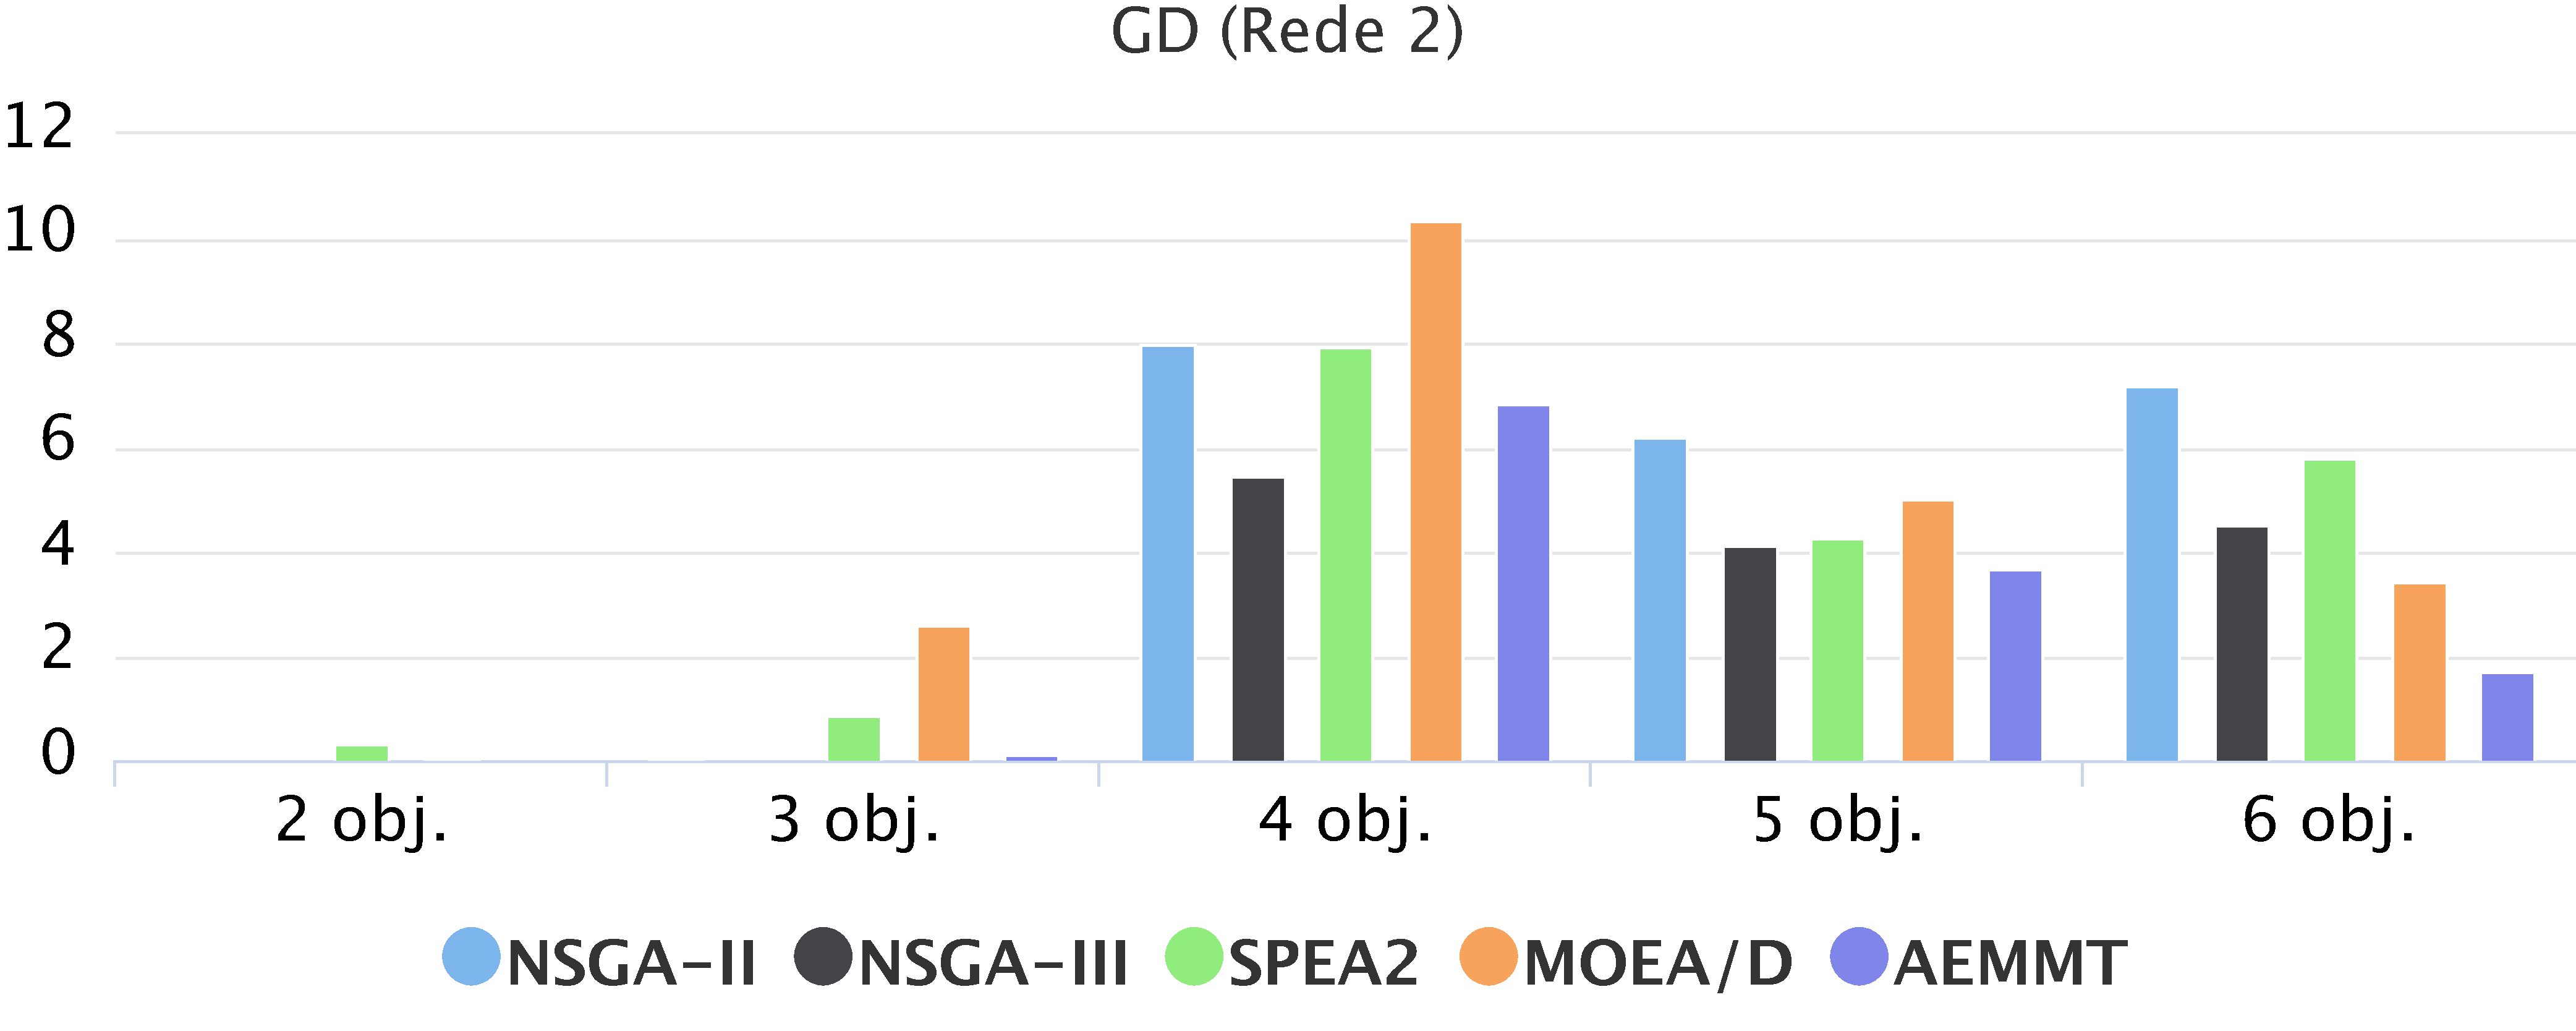
\includegraphics[width=1\textwidth]{cap_experimentos/figs/etapa1/gd-mrp-r2}
	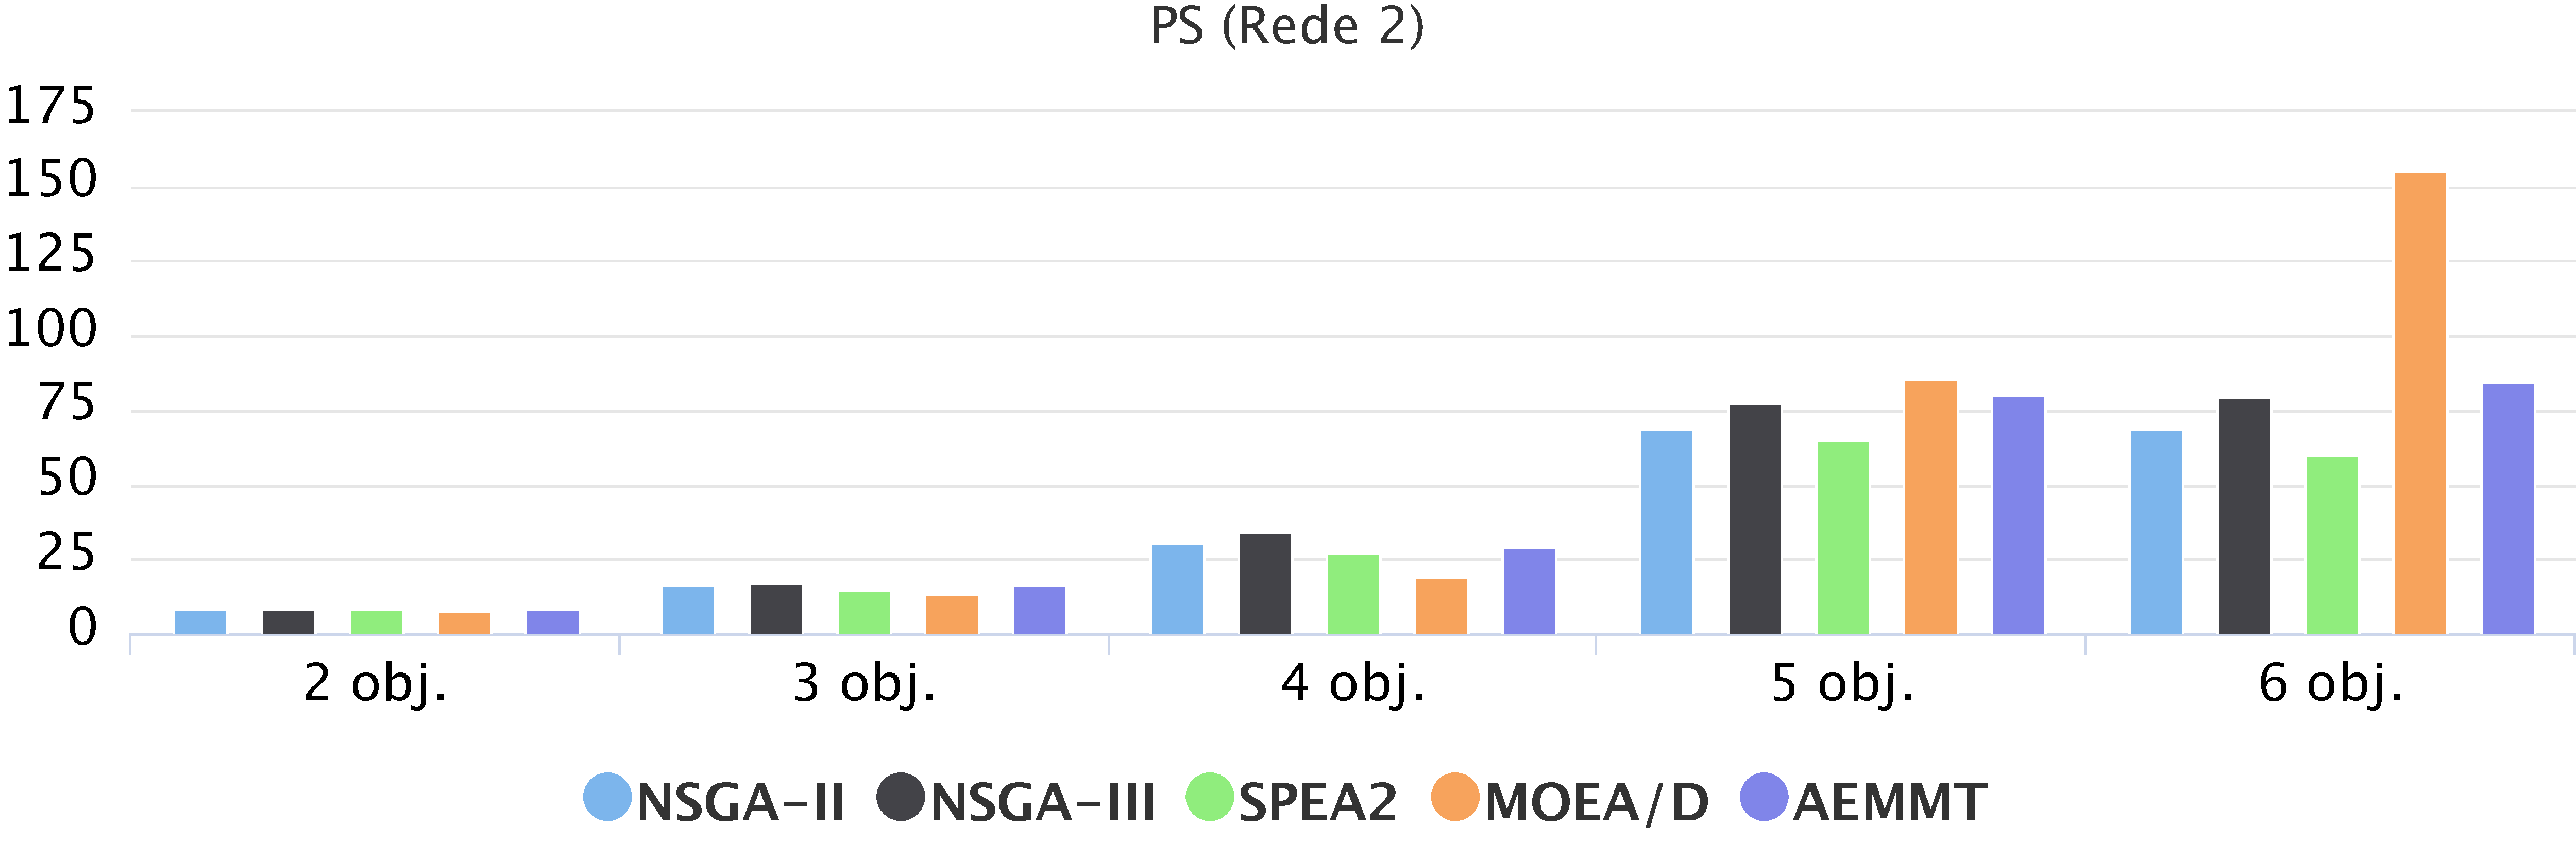
\includegraphics[width=1\textwidth]{cap_experimentos/figs/etapa1/ps-mrp-r2}
\end{figure*}

Na rede 2 (figura \ref{fig_exp1_mrp_r2}), o NSGA-III é o melhor algoritmo nos problemas com 2, 3, 4 e 5 objetivos, perdendo, por pouco, apenas em $PS$ para o AEMMT e o MOEA/D no problema de 5 objetivos. Com 6 objetivos, o AEMMT é o melhor algoritmo quando se considera o erro e o $GD$, mas se um maior $PS$ é mais desejável, então o MOEA/D é o método mais adequado.

\begin{figure*}[!htbp]
	\caption{Etapa 1: resultados para o PRM na rede $R_3$}
	\label{fig_exp1_mrp_r3}
	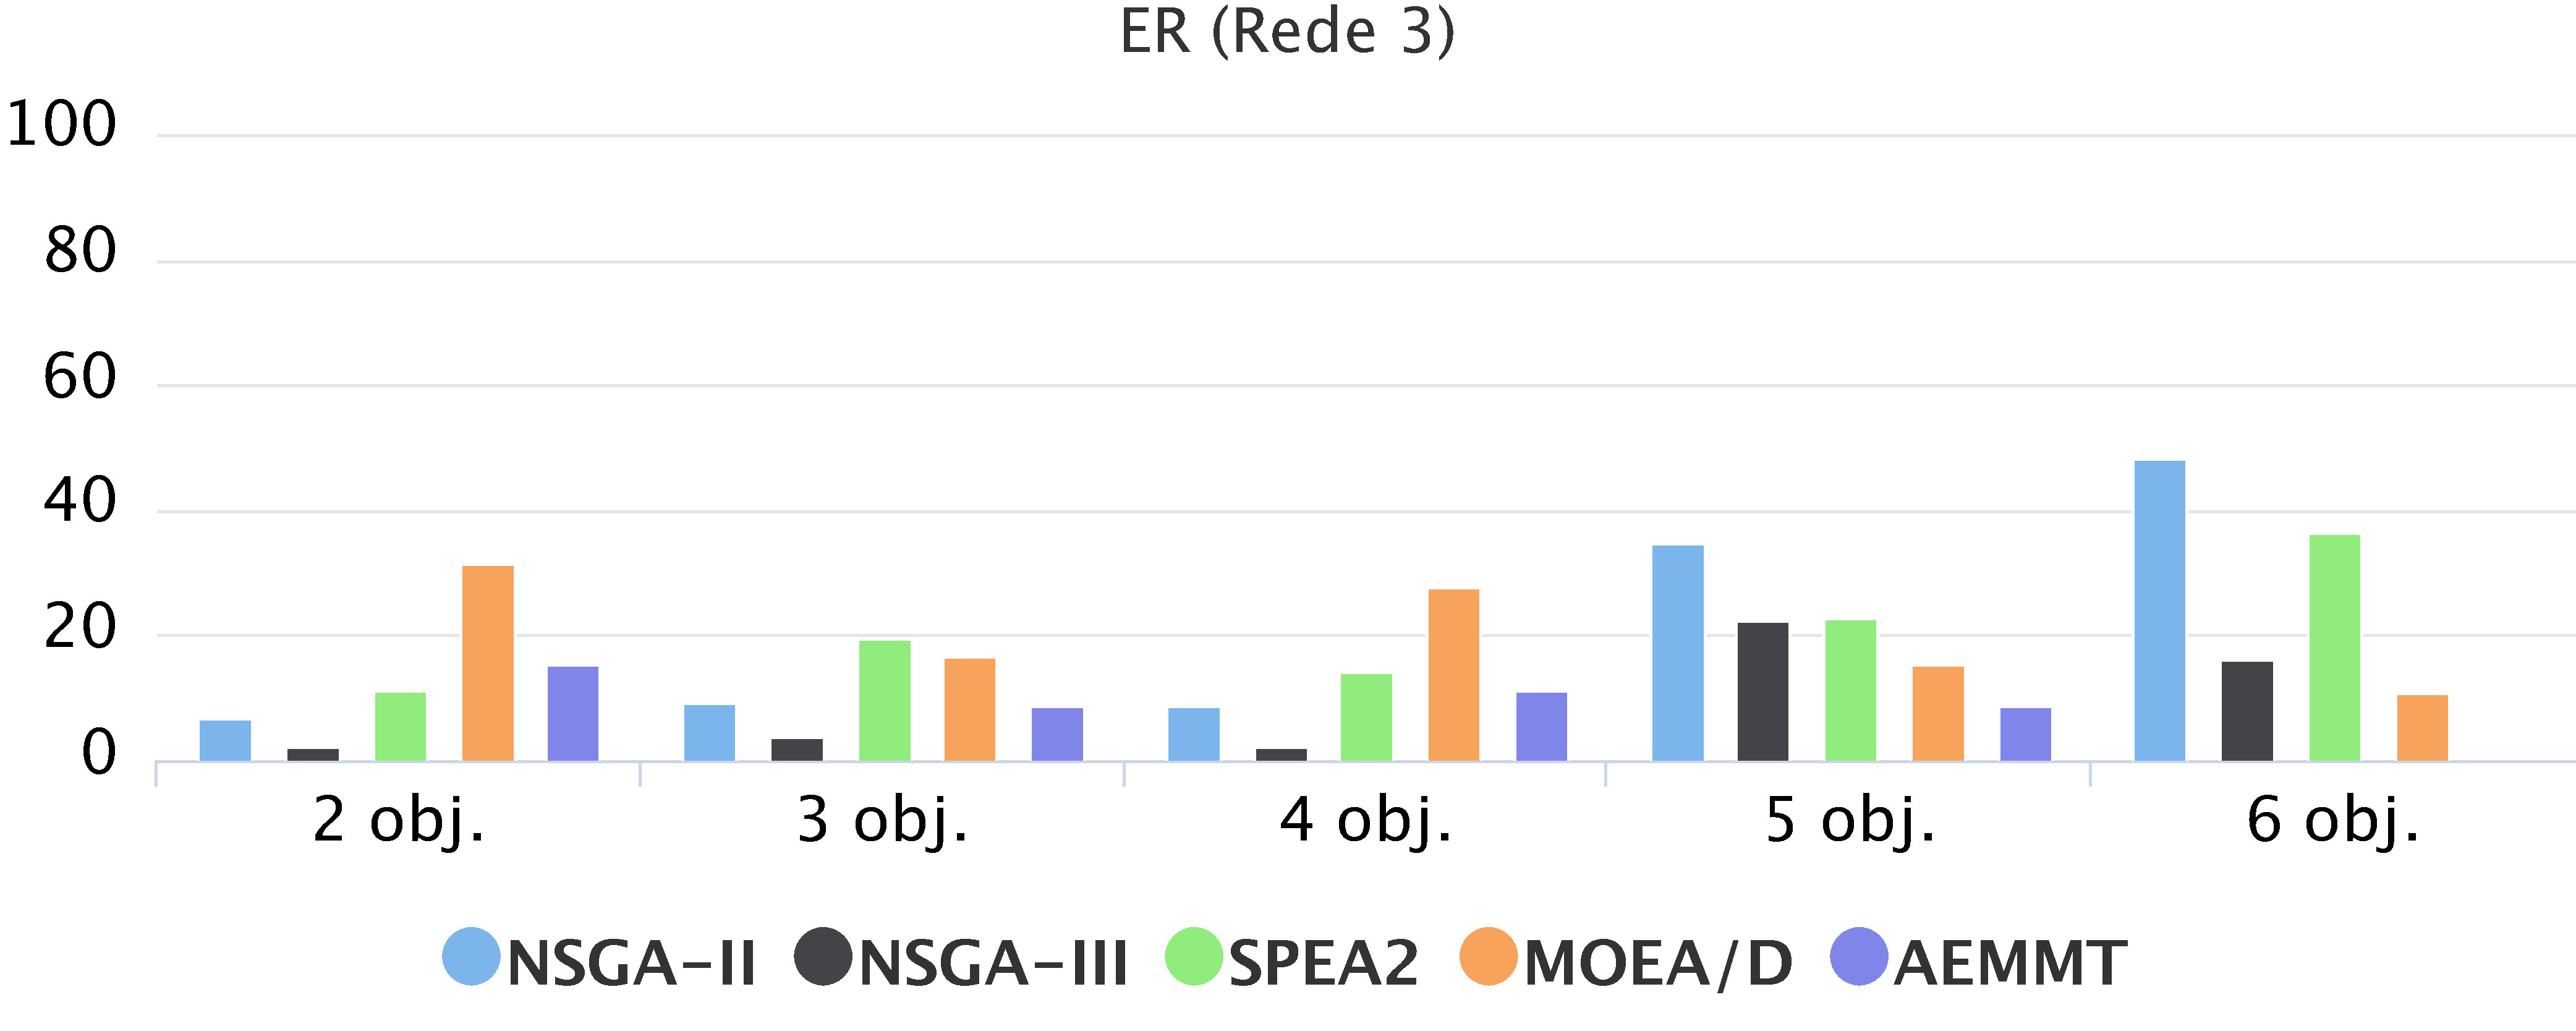
\includegraphics[width=1\textwidth]{cap_experimentos/figs/etapa1/er-mrp-r3}
	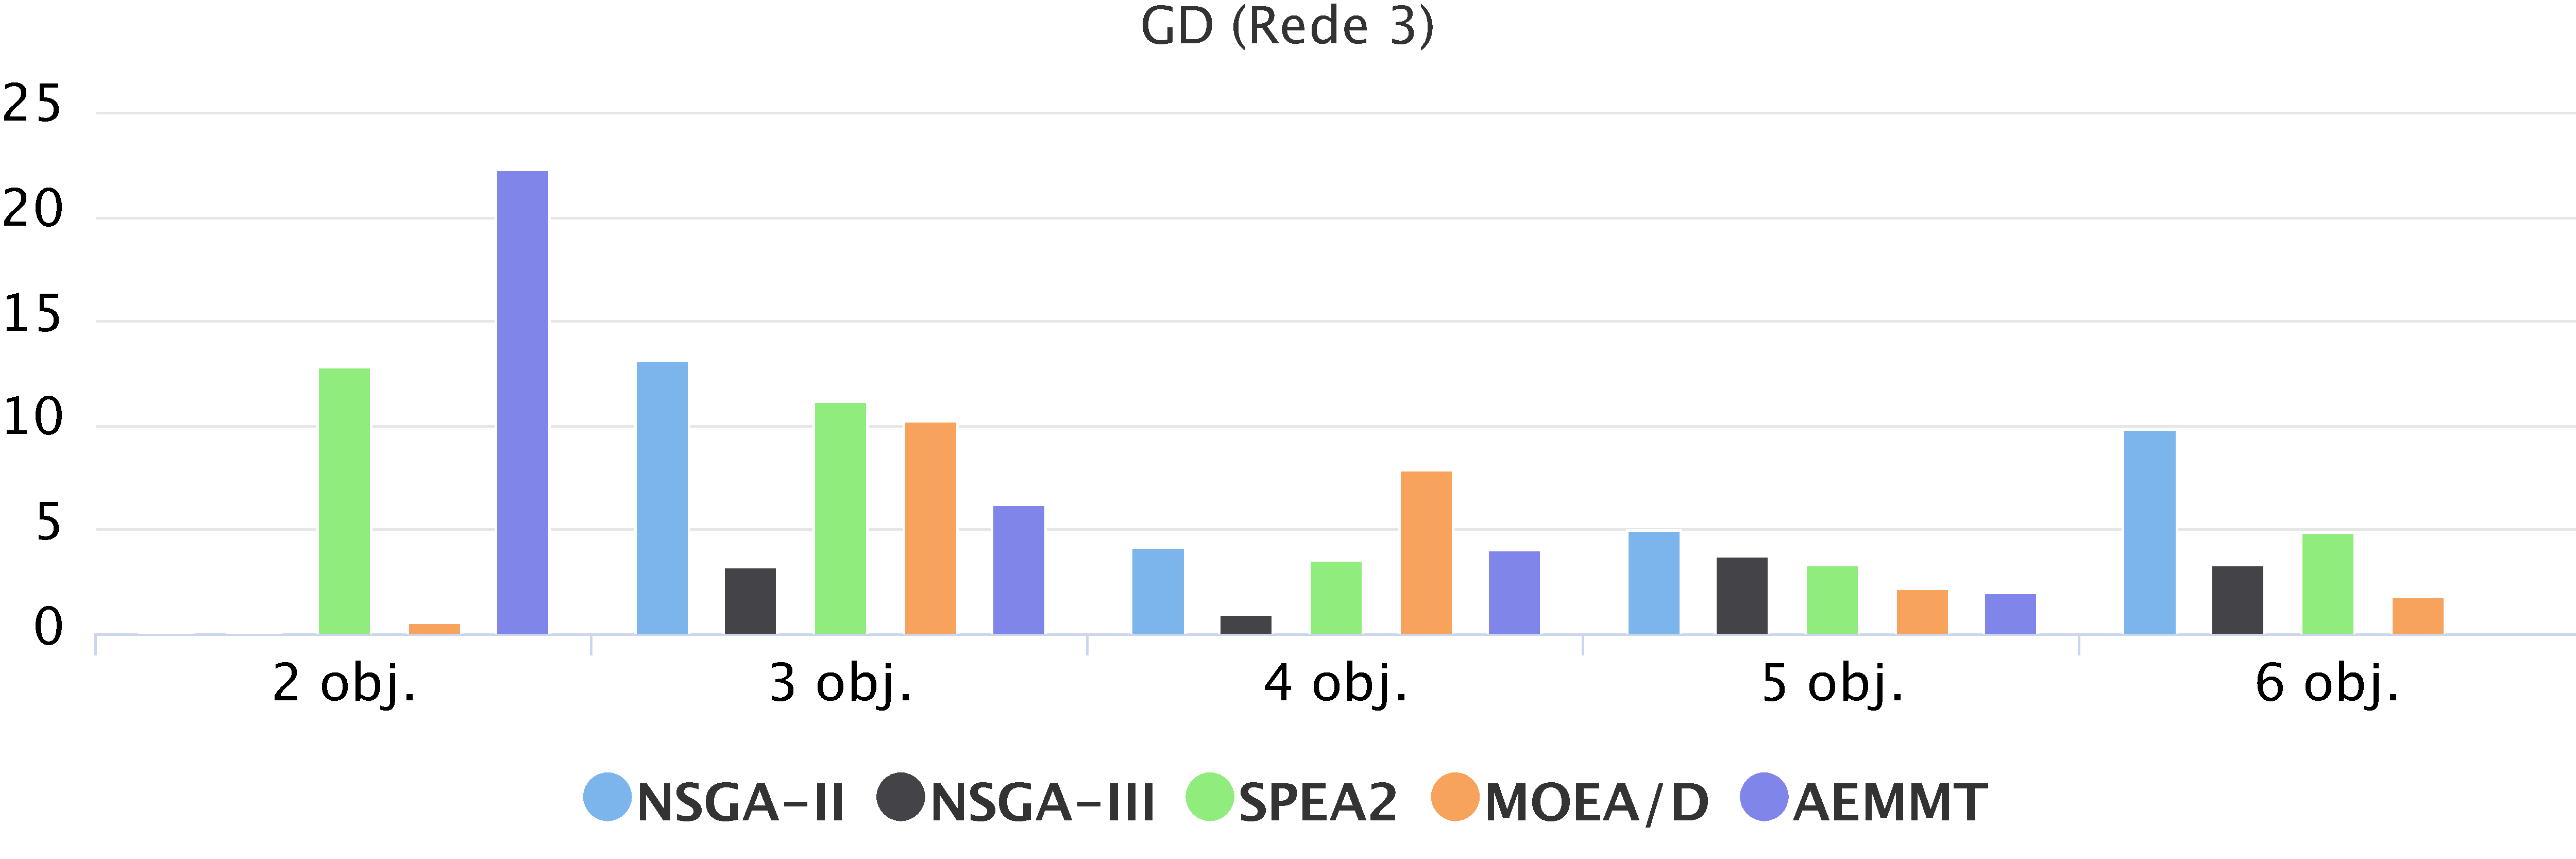
\includegraphics[width=1\textwidth]{cap_experimentos/figs/etapa1/gd-mrp-r3}
	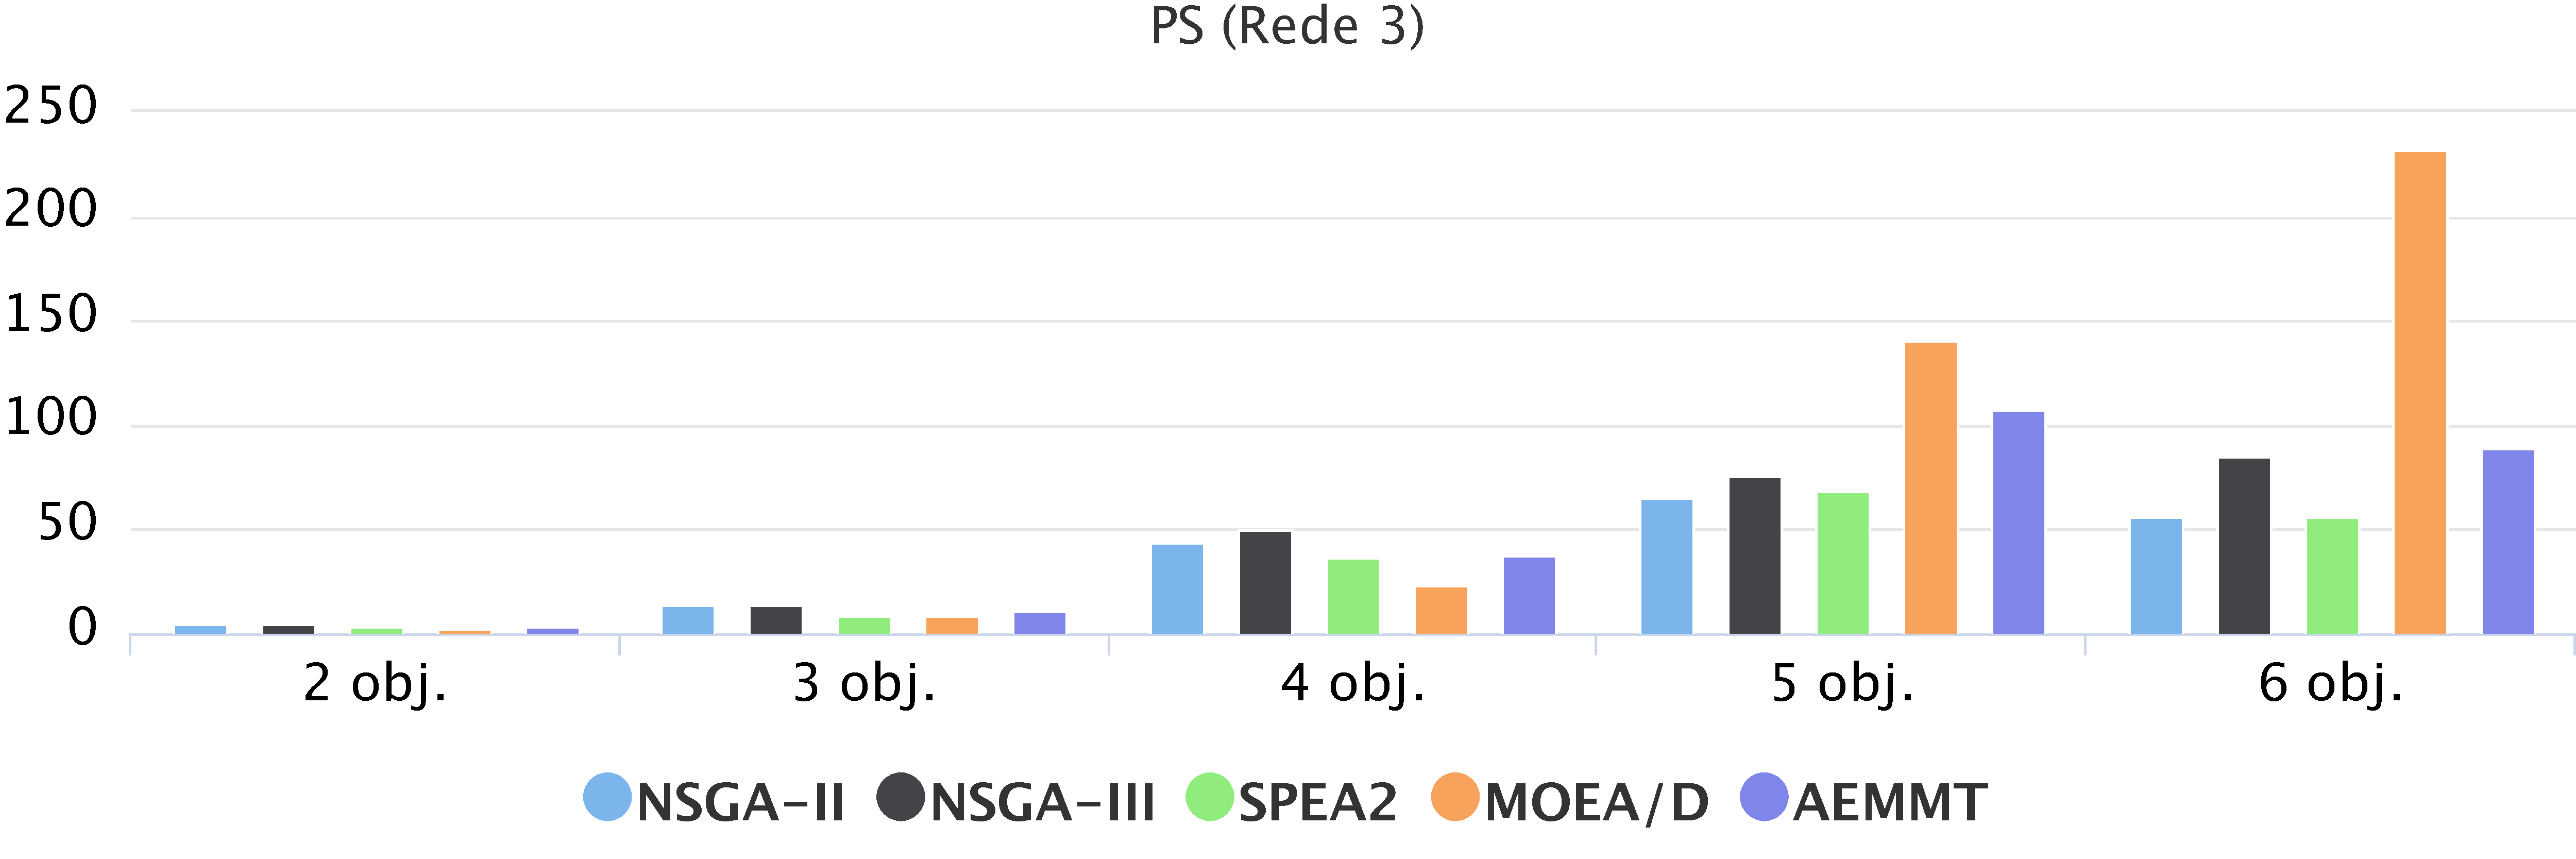
\includegraphics[width=1\textwidth]{cap_experimentos/figs/etapa1/ps-mrp-r3}
\end{figure*}

A rede 3 (figura \ref{fig_exp1_mrp_r3}) é a mais complexa analisada nesta etapa dos experimentos. Nela, a tendência já observada do NSGA-III de ser o melhor método para poucos objetivos continua. Até 4 objetivos, em todas as métricas, o NSGA-III apresenta os melhores resultados. Para 5 e 6 critérios de otimização, o AEMMT apresenta menor $ER$ e $GD$, enquanto o MOEA/D consegue maior $PS$.

\begin{figure*}[!htbp]
	\caption{Etapa 1: resultados agrupados para o PRM nas redes $R_1$, $R_2$ e $R_3$}
	\label{fig_exp1_mrp_todos}
	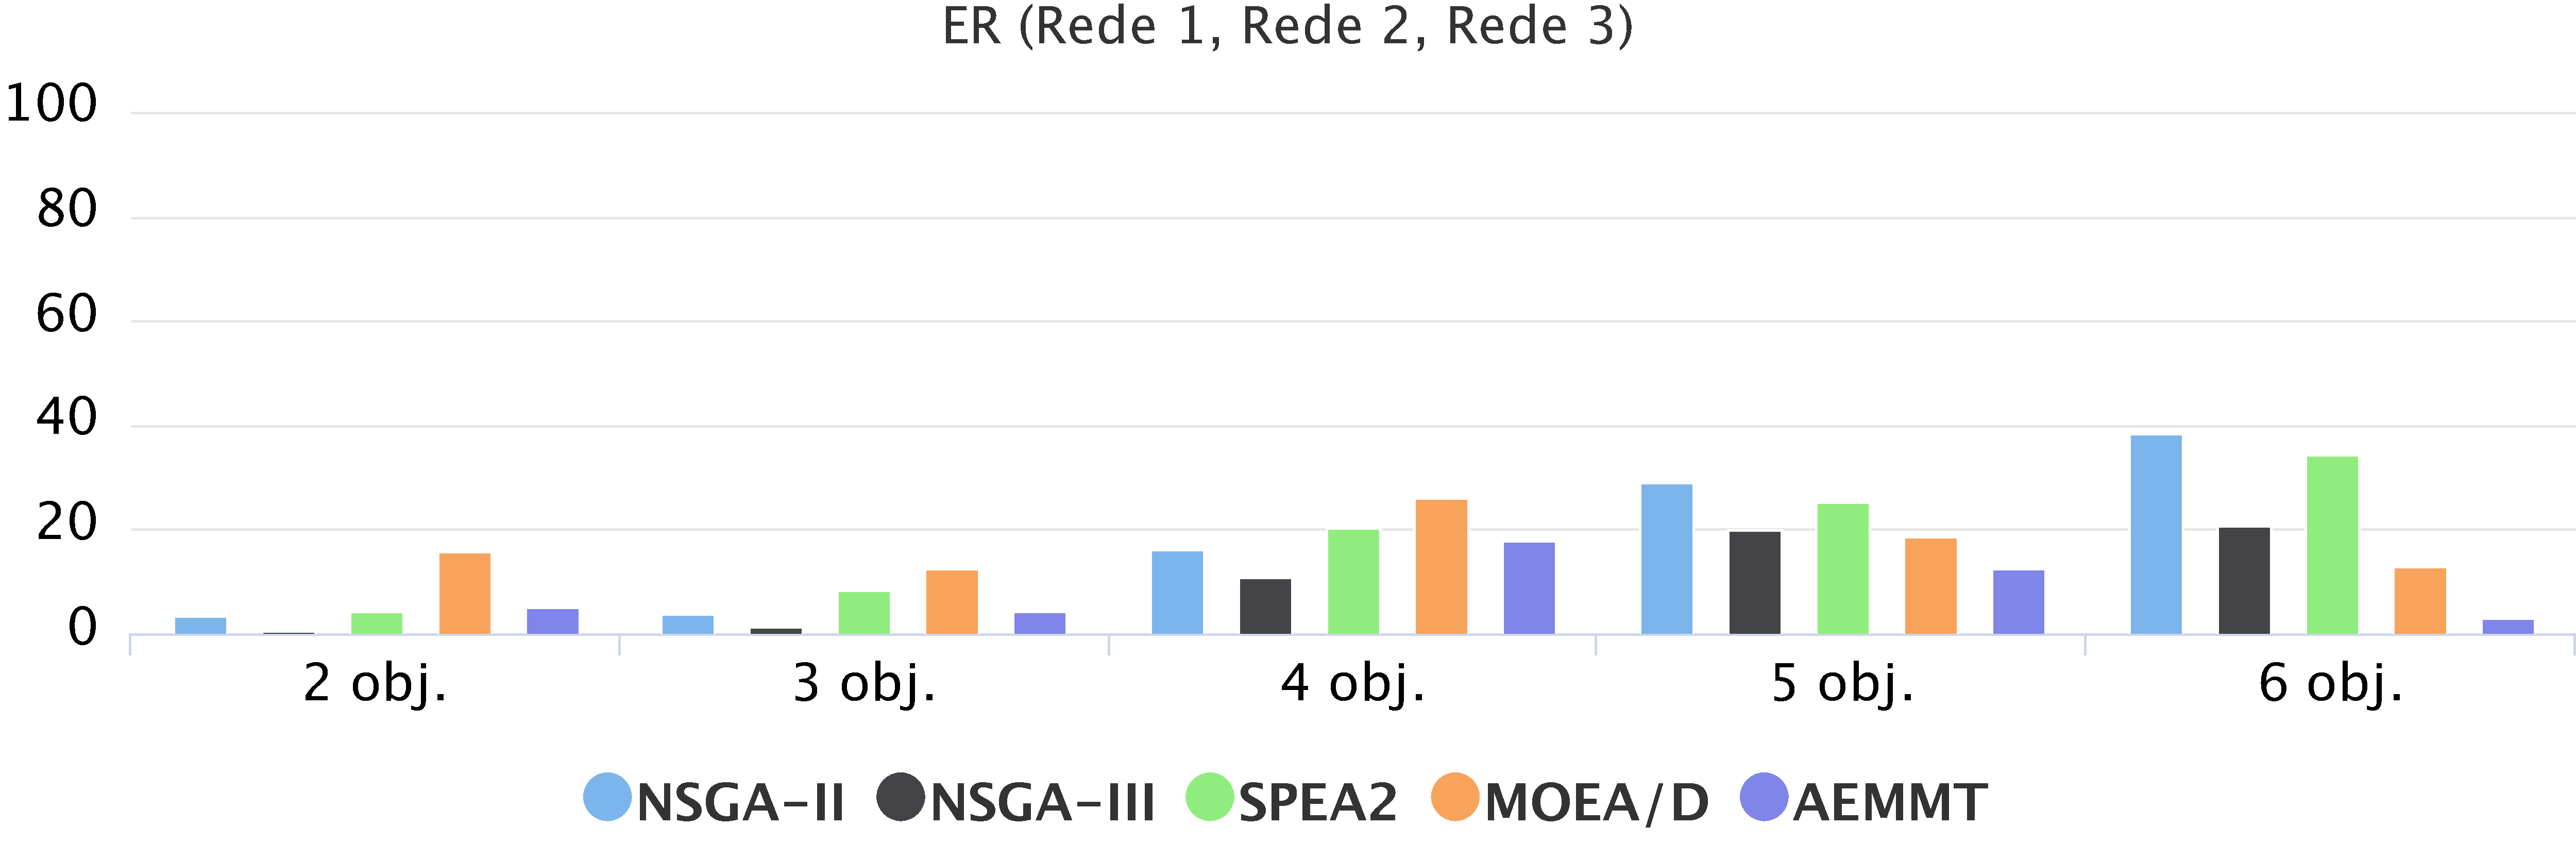
\includegraphics[width=1\textwidth]{cap_experimentos/figs/etapa1/er-mrp-todos}
	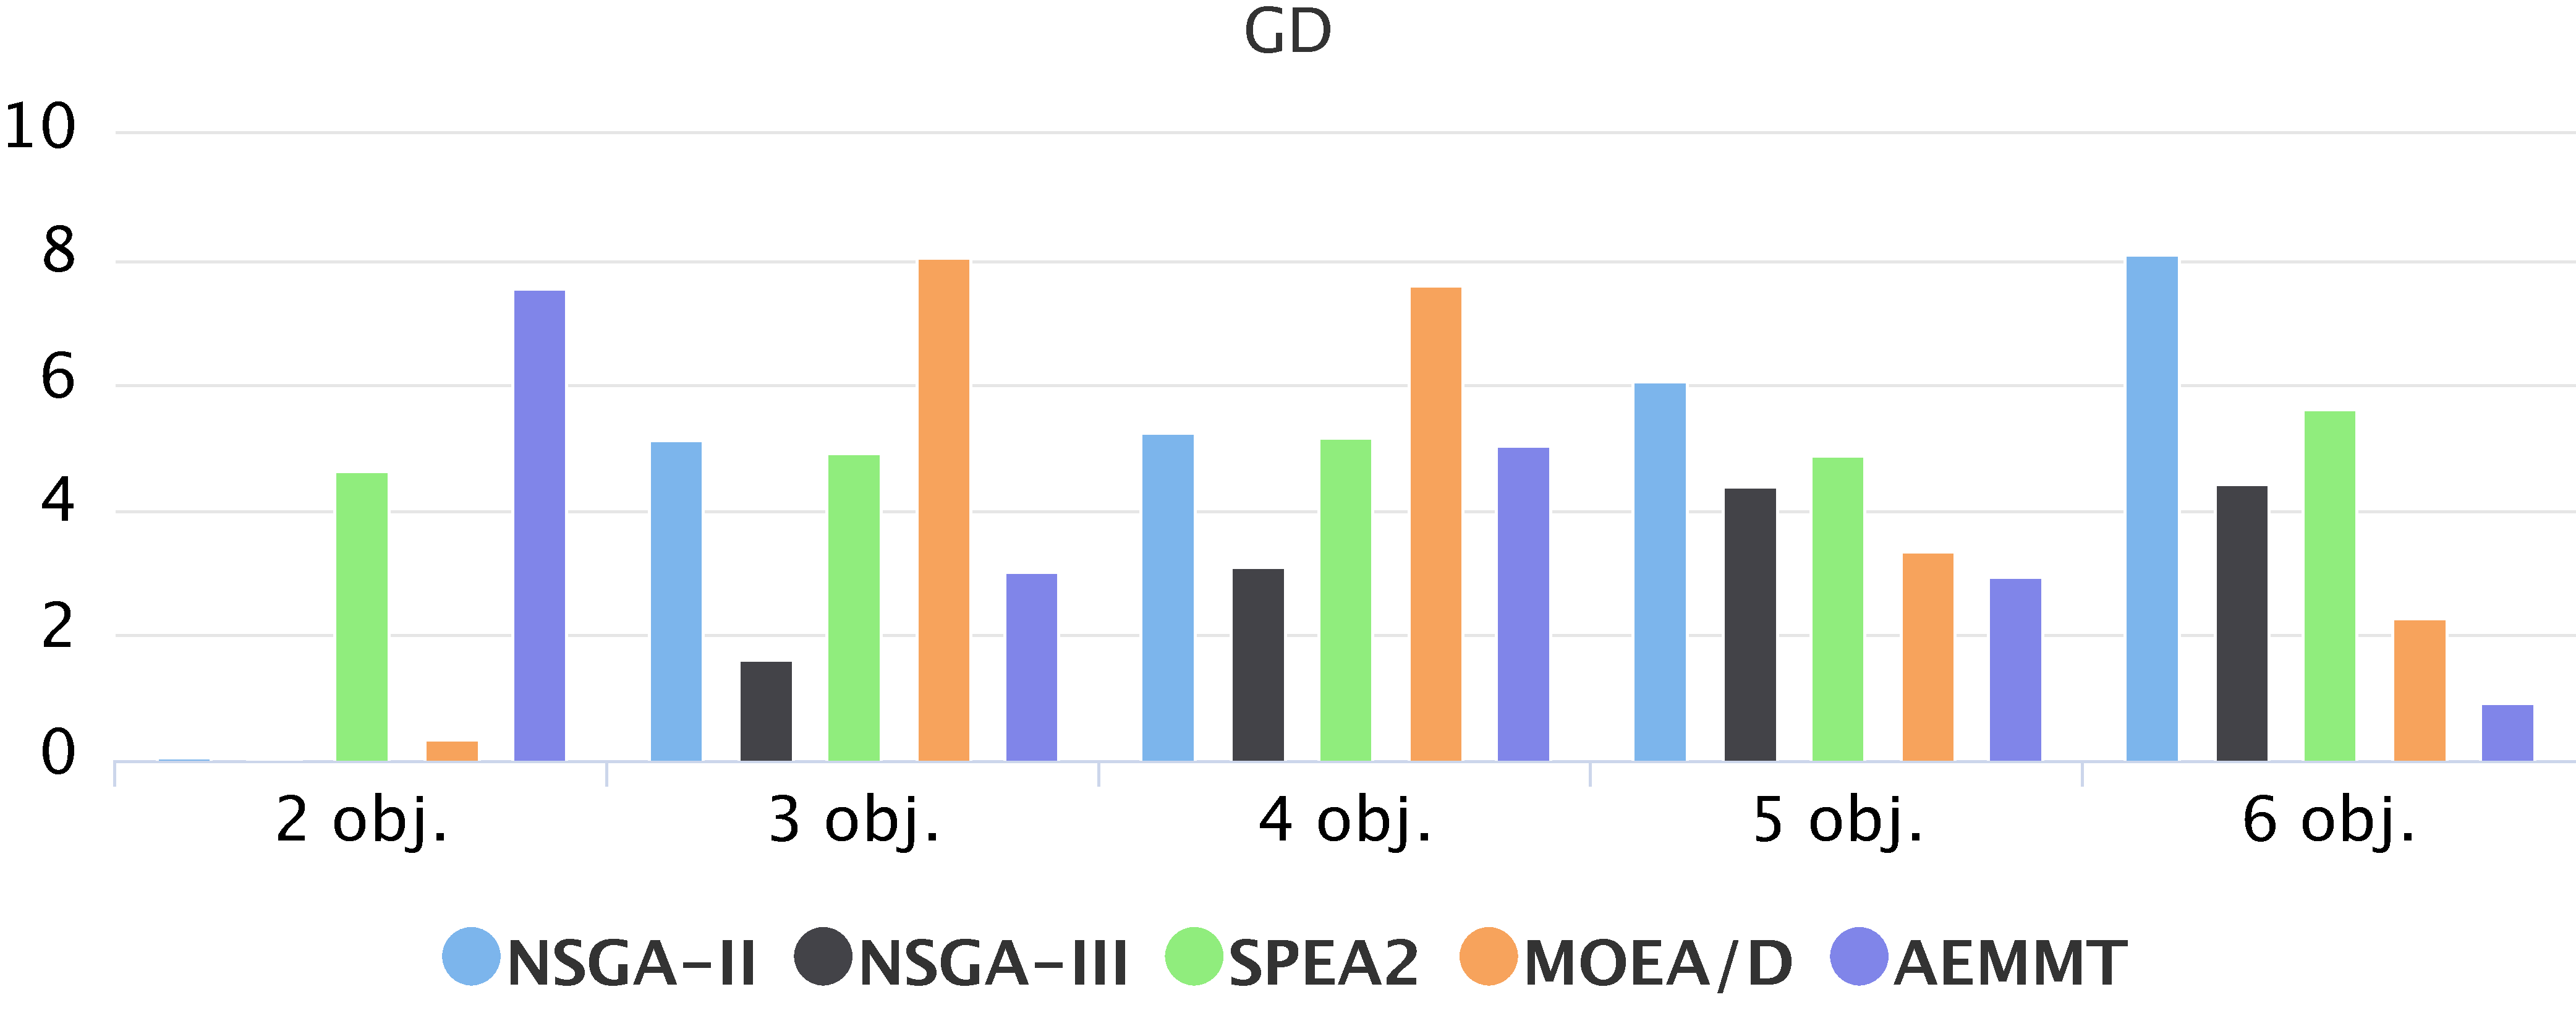
\includegraphics[width=1\textwidth]{cap_experimentos/figs/etapa1/gd-mrp-todos}
	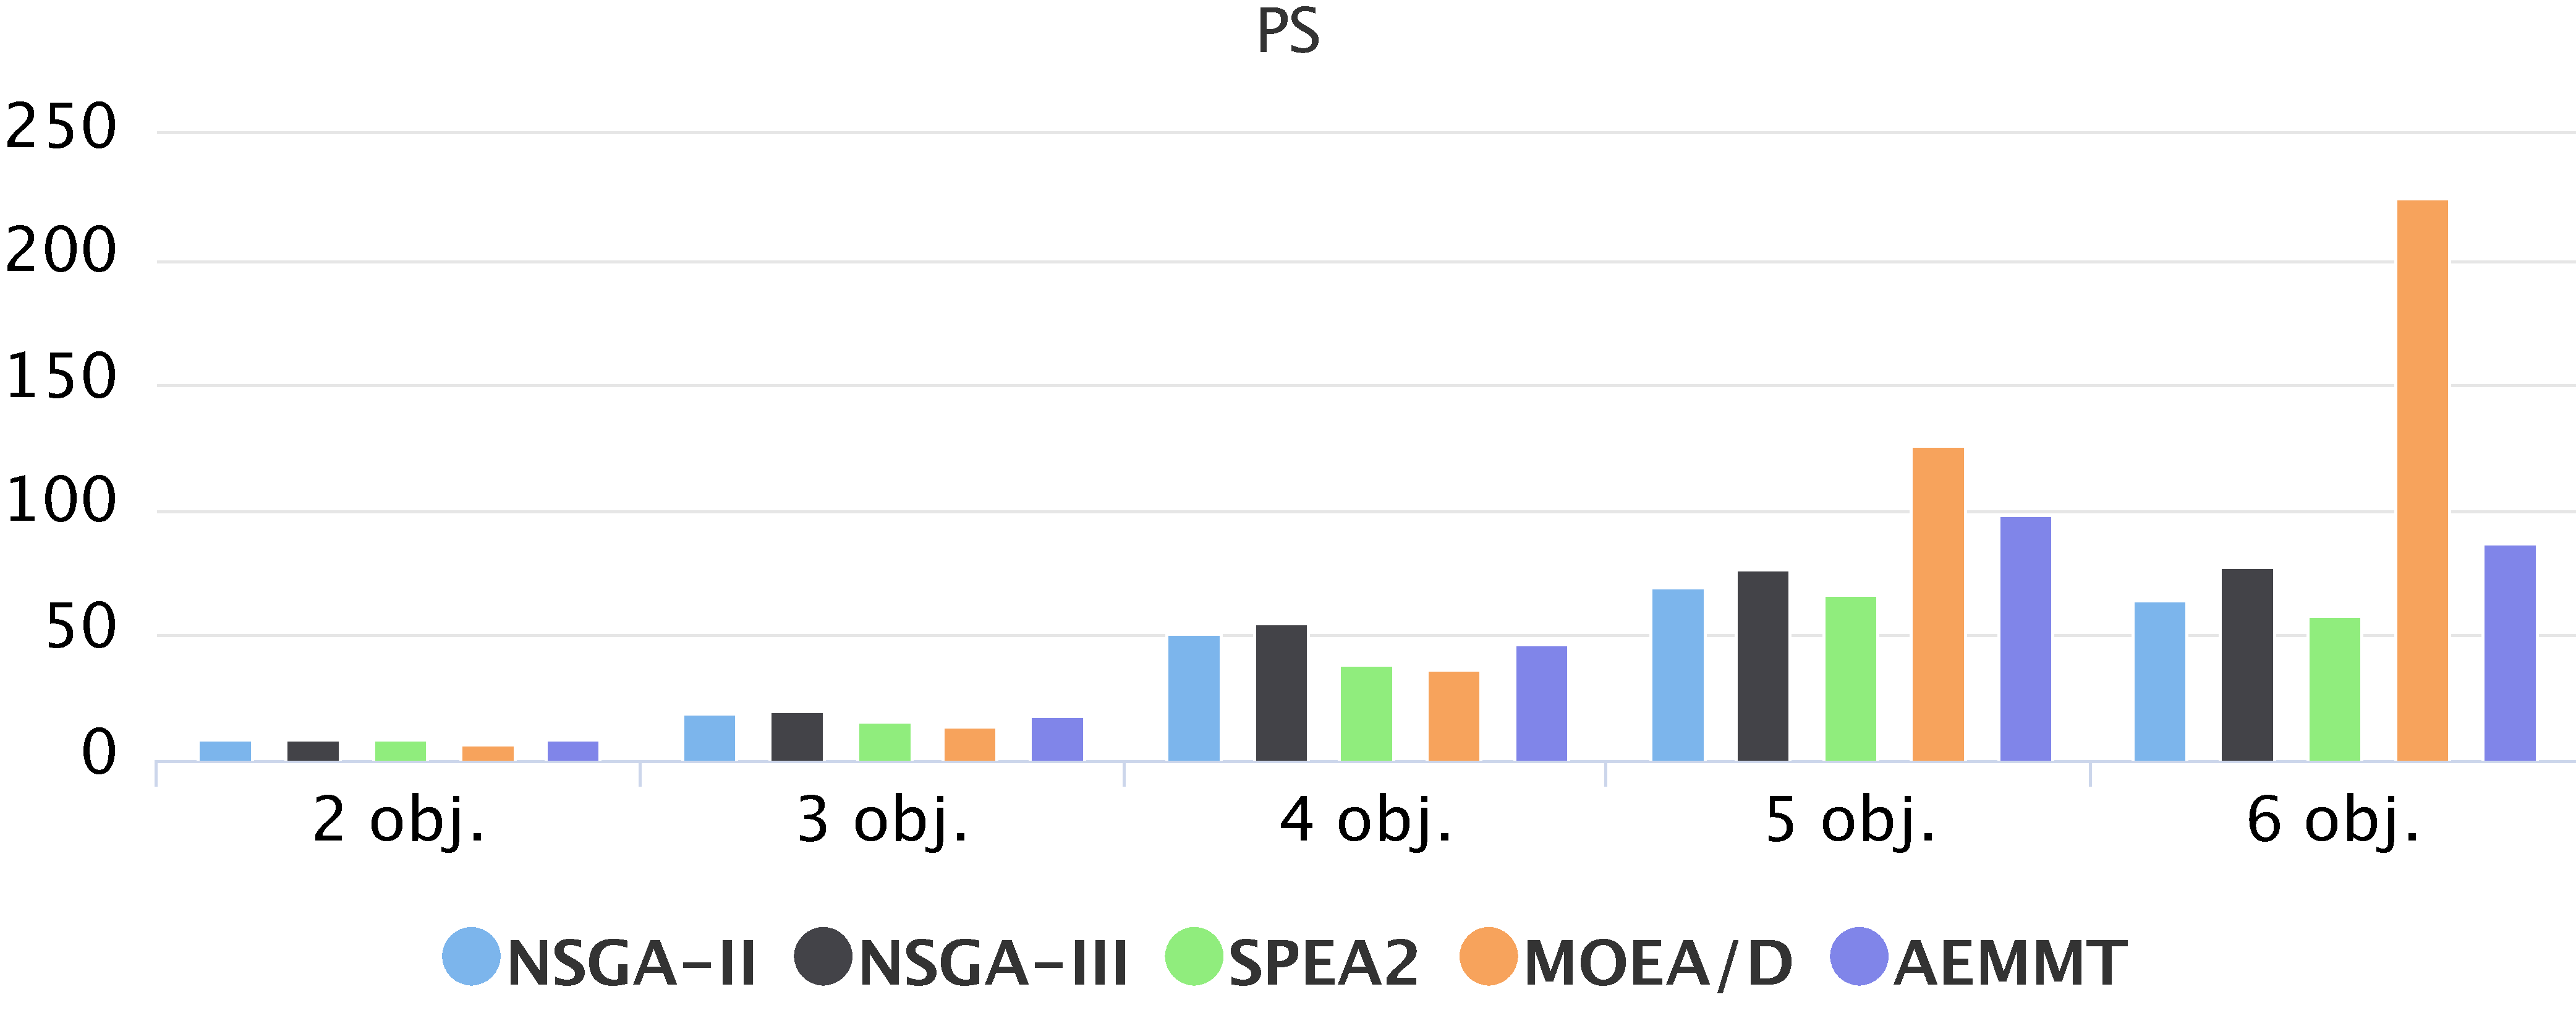
\includegraphics[width=1\textwidth]{cap_experimentos/figs/etapa1/ps-mrp-todos}
\end{figure*}

Afim de fazer uma análise geral do PRM, na figura \ref{fig_exp1_mrp_todos}, todos os cenários (redes 1, 2 e 3) são combinados num único gráfico através de uma média aritmética dos resultados. Observa-se que, apesar de ser esperado que o NSGA-II e o SPEA2 fossem os melhores métodos para poucos objetivos, na verdade, o NSGA-III foi o algoritmo que obteve melhor resultado para problemas com, 2, 3 e 4 objetivos. O NSGA-II também produz bons resultados para problemas com 2 e 3 objetivos, mas o SPEA2 apresenta um $GD$ relativamente ruim. Considerando problemas de 5 e 6 objetivos, a escolha do algoritmo dependerá do intuito da busca, se é preferível uma maior quantidade de soluções, o MOEA/D é mais indicado, caso contrário, se um menor erro é preferível, então o AEMMT é a melhor opção.

Considerando ambos os problemas, PMM e PRM, os algoritmos NSGA-II, SPEA2 e NSGA-III são os que geram melhores resultados para problemas com poucos objetivos. A performance dos algoritmos clássicos (NSGA-II e SPEA2) cai consideravelmente a medida que se aumenta o número de objetivos, enquanto o desempenho dos métodos AEMMT e MOEA/D melhora a partir de quatro objetivos, tornando-nos os mais indicados para problemas \textit{many-objectives}.

Uma outra observação que pôde ser feita a partir dos experimentos nesta etapa é que o AEMMT perde apenas em $PS$ para o MOEA/D. Uma das características do AEMMT é a limitação no tamanho do arquivo, por isso surge a dúvida: se não houvesse um limite, seria possível que o AEMMT obtivesse um melhor resultado em todas as métricas. Pensando nisso, executou-se os mesmos testes para uma variação do AEMMT (AEMMT-F) onde o limite não foi aplicado. Na maioria dos resultados, o AEMMT-F apresentou erro maior que sua versão original, mas ainda sim $ER$ e $PS$ melhores que o MOEA/D. Dessa forma, através de um teste de hipótese z-teste com 0,1\% de significância ($\alpha = 0.1$), confirmou-se a superioridade do AEMMT-F em relação ao MOEA/D nos cenários com 5 e 6 objetivos.

\section{Etapa 2: AG's many-objectives vs. MACO/D}

Na segunda etapa de experimentos descartam-se os AEMOs clássicos NSGA-II e SPEA2 e inclui-se o AEMMD e o MACO/D, algoritmo proposto neste trabalho. Uma nova métrica de desempenho é utilizada, o tempo, e as demais continuam sendo o erro ($ER$), a distância ($GD$) e o número de soluções corretas ($PS$). Assim como na etapa 1, o Pareto aproximado foi pré-calculado a partir de múltiplas execuções dos algoritmos e é apresentado na tabela \ref{table_exp2_paretos}. Enfim, os resultados (com exceção do tempo) foram obtidos através das médias entre 100 execuções dos 30 cenários descritos na lista a seguir. A medida de tempo considerou apenas 3 execuções de cada algoritmo em cada cenário.

\begin{itemize}
	\item PRM: 3 formulações de objetivos ($P_4$, $P_5$ e $P_6$) e 3 redes ($R_1$, $R_2$ e $R_3$). Tanto as formulações quanto às redes foram descritas na seção correspondente ao problema do roteamento multicast [].
	\item PMM: 3 formulações de objetivos (4 a 6) e 3 instâncias (30, 40 e 50 itens).
\end{itemize}


\begin{table}[!htbp]
	\centering
	\caption{Cardinalidade dos Paretos encontrados para a primeira etapa de experimentos}
	\label{table_exp2_paretos}
	\begin{tabular}{c|rrr|rrr}
		& \multicolumn{3}{c|}{\textbf{PRM}} & \multicolumn{3}{c}{\textbf{PMM}} \\ \hline
		Objetivos & R1         & R2       & R3        & 30 itens  & 50 itens & 100 itens \\ \hline
		4         & 122        & 553       & 1349        & 425       & 1199      & 1012    \\
		5         & 75        & 372      & 712       & 1769      & 3862     & 5467   \\
		6         & 70       & 660      & 1283      & 5828      & 6491   & 55471   \\ \hline
	\end{tabular}
\end{table}

A tabela \ref{table_exp2_parametros} apresenta os parâmetros dos algoritmos utilizados neste experimento. Note que o número de gerações (marcado com asterisco) deve ser multiplicado pelo tamanho da população no AEMMT e AEMMD devido ao fato de realizarem apenas um crossover por geração.

\begin{table}[!htbp]
	\caption{Parâmetros utilizados para o PRM e o PMM.}
	\label{table_exp2_parametros}
	\begin{center}
		\begin{tabular}{c|r|r}
			\textbf{Parâmetro} & \textbf{PRM} &  \textbf{PMM} \\ %\hline
			\hline
			Tamanho da população               &    90 &      150 \\ %\hline
			Número de gerações*        &   100 &      100 \\ %\hline
			Taxa de crossover                & 100\% &    100\% \\ %\hline
			Taxa de mutação                 &  20\% &      5\% \\ %\hline
			Tamanho da vizinhança (MOEA/D)    &    10 &       10 \\ %\hline
			Tamanho das tabelas (MEAMT)   &    30 &       50 \\ %\hline
			Tamanho da tabela de dominância (MEAMT) &    90 &      150 \\ %\hline
			Número de divisões (NSGA-III)&     8 &        8 \\ %\hline
			$\alpha, \beta, \rho$ (MACO/D)& 1, 2, 0.3 & 1, 4.3, 0.3 \\ %\hline
			Intervalo de valores para os feromônios (MACO/D)& [0.1, 0.9] & [0.1, 0.9] \\ %\hline
			Tamanho das amostras (MACO/D)& 10 &25\% of the number of items \\  %\hline
			Tamanho do grupo de estruturas ativas (MACO/D)& 5 & 5 \\
			\hline
		\end{tabular}
	\end{center}
\end{table}

As figuras \ref{fig_exp2_pmm_30}, \ref{fig_exp2_pmm_40} e \ref{fig_exp2_pmm_50} mostram respectivamente os resultados para o PMM de 30, 40 e 50 itens. As figuras \ref{fig_exp2_prm_r1}, \ref{fig_exp2_prm_r2} e \ref{fig_exp2_prm_r3} revelam respectivamente os resultados para o PRM aplicado às redes $R_1$, $R_2$ e $R_3$. Uma análise conjunta, com uma média entre as três instâncias de cada problema é apresenta nas figuras \ref{fig_exp2_prm_todos} (PRM) e \ref{fig_exp2_pmm_todos} (PMM).

\begin{figure*}[!htbp]
	\caption{Etapa 2: resultados para o PMM com 30 itens}
	\label{fig_exp2_mkp_30}
	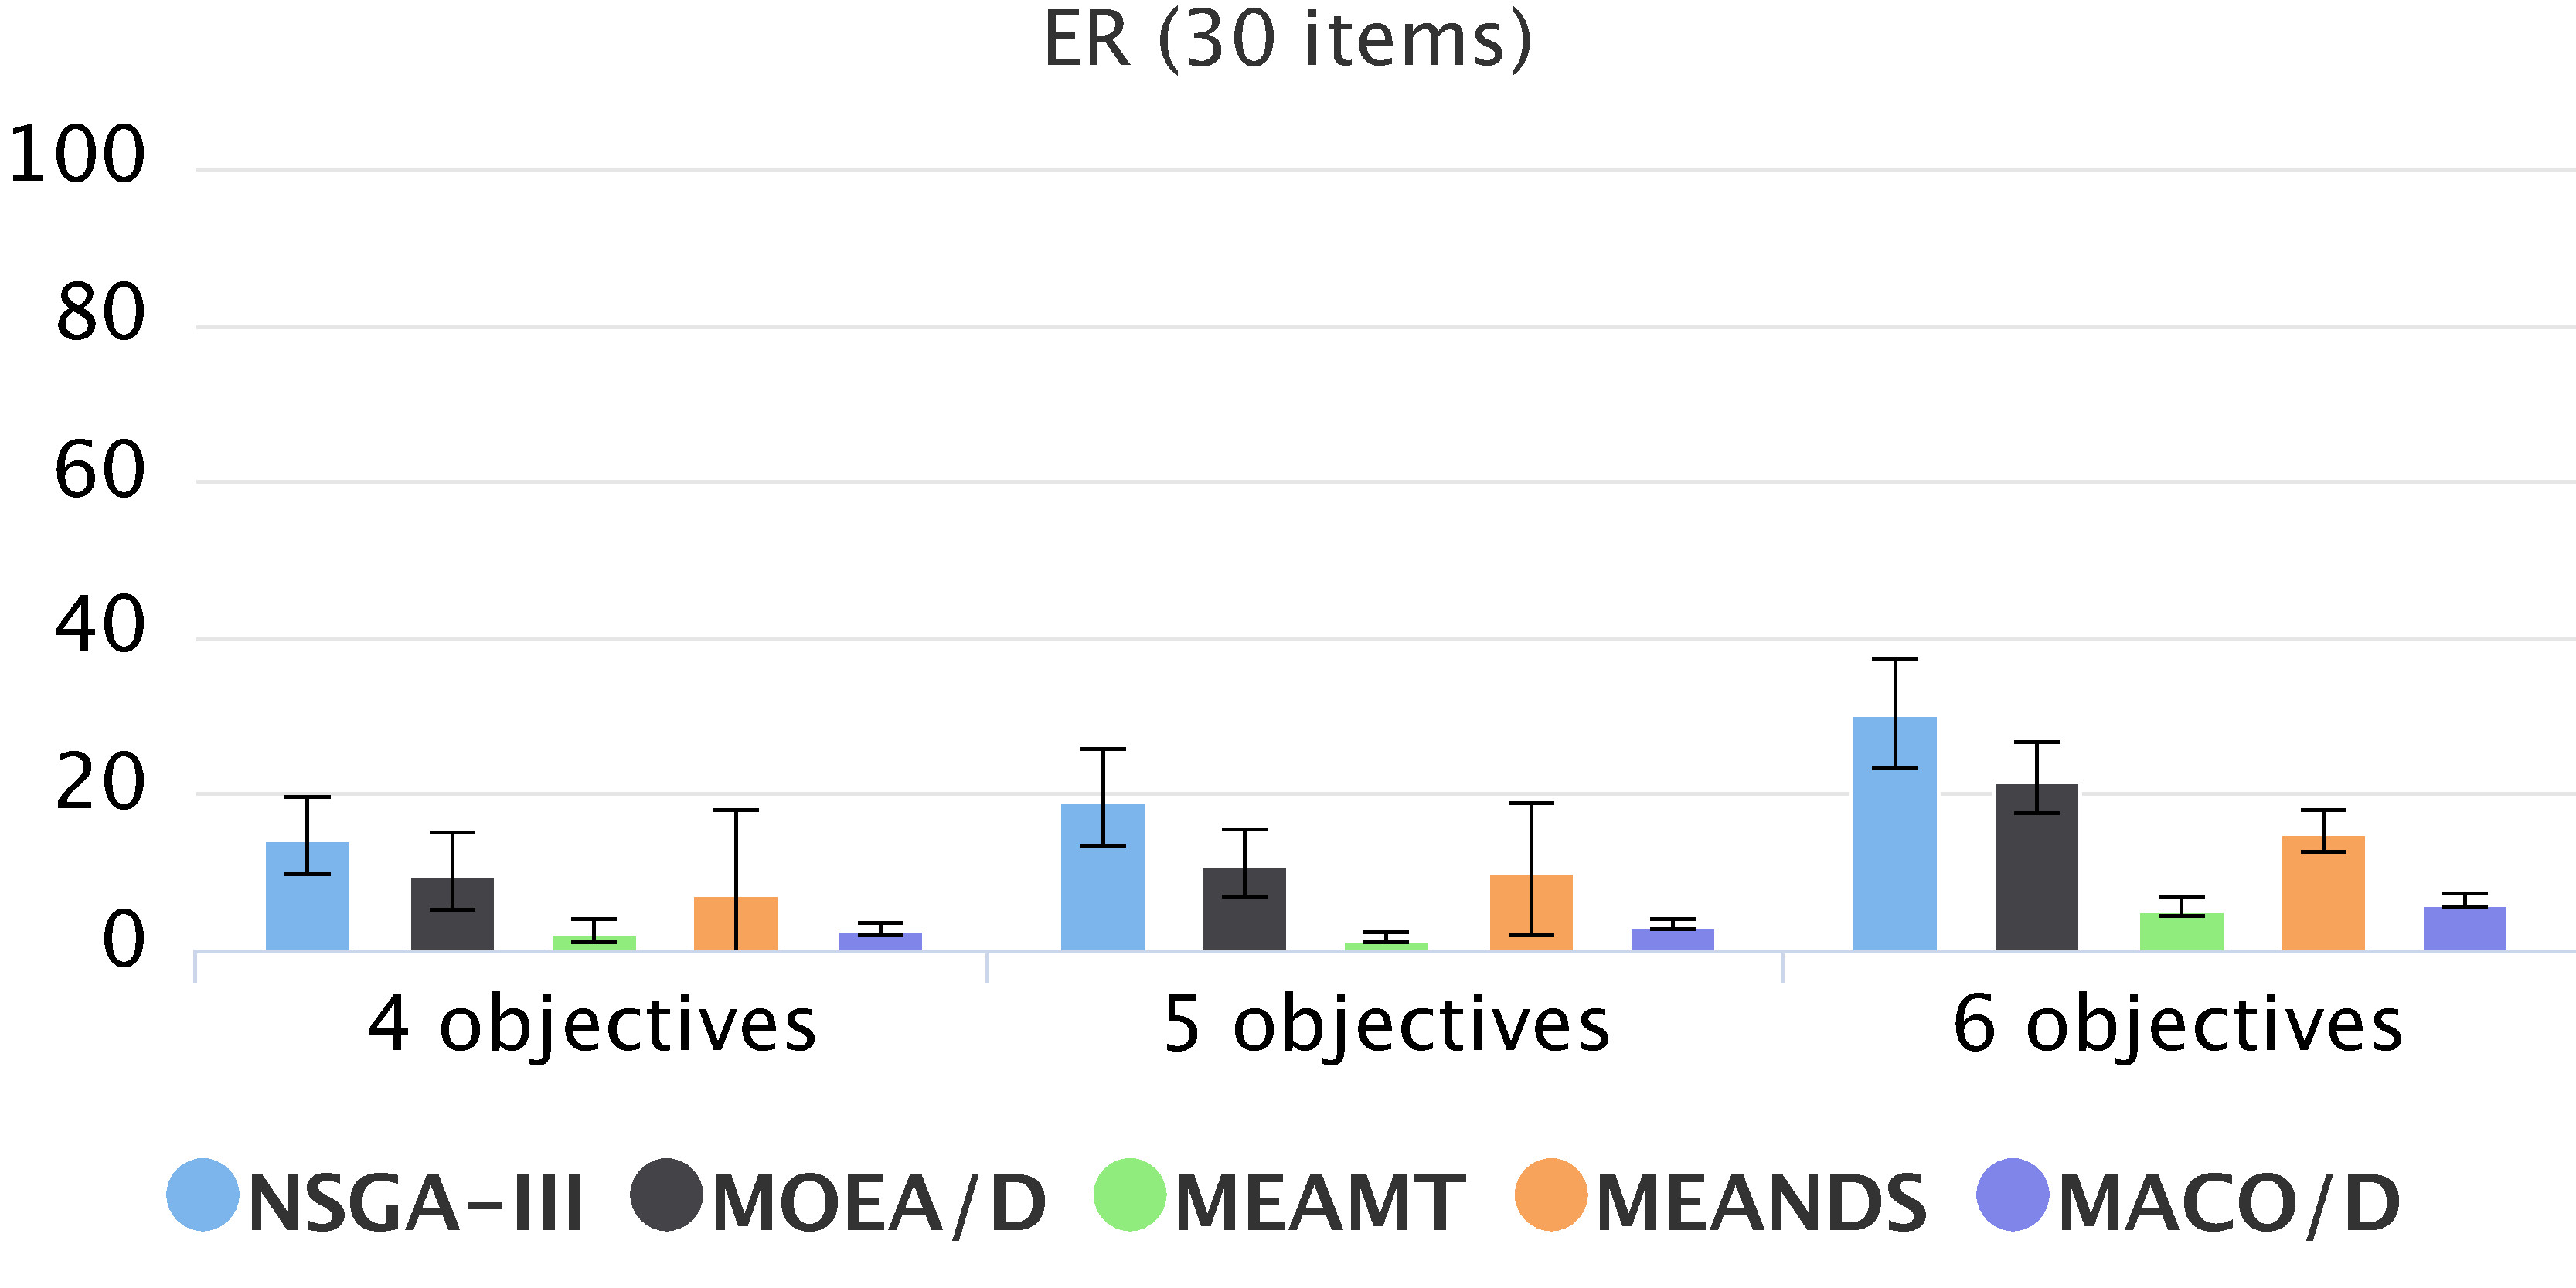
\includegraphics[width=0.5\textwidth]{cap_experimentos/figs/etapa2/er-mkp-30}
	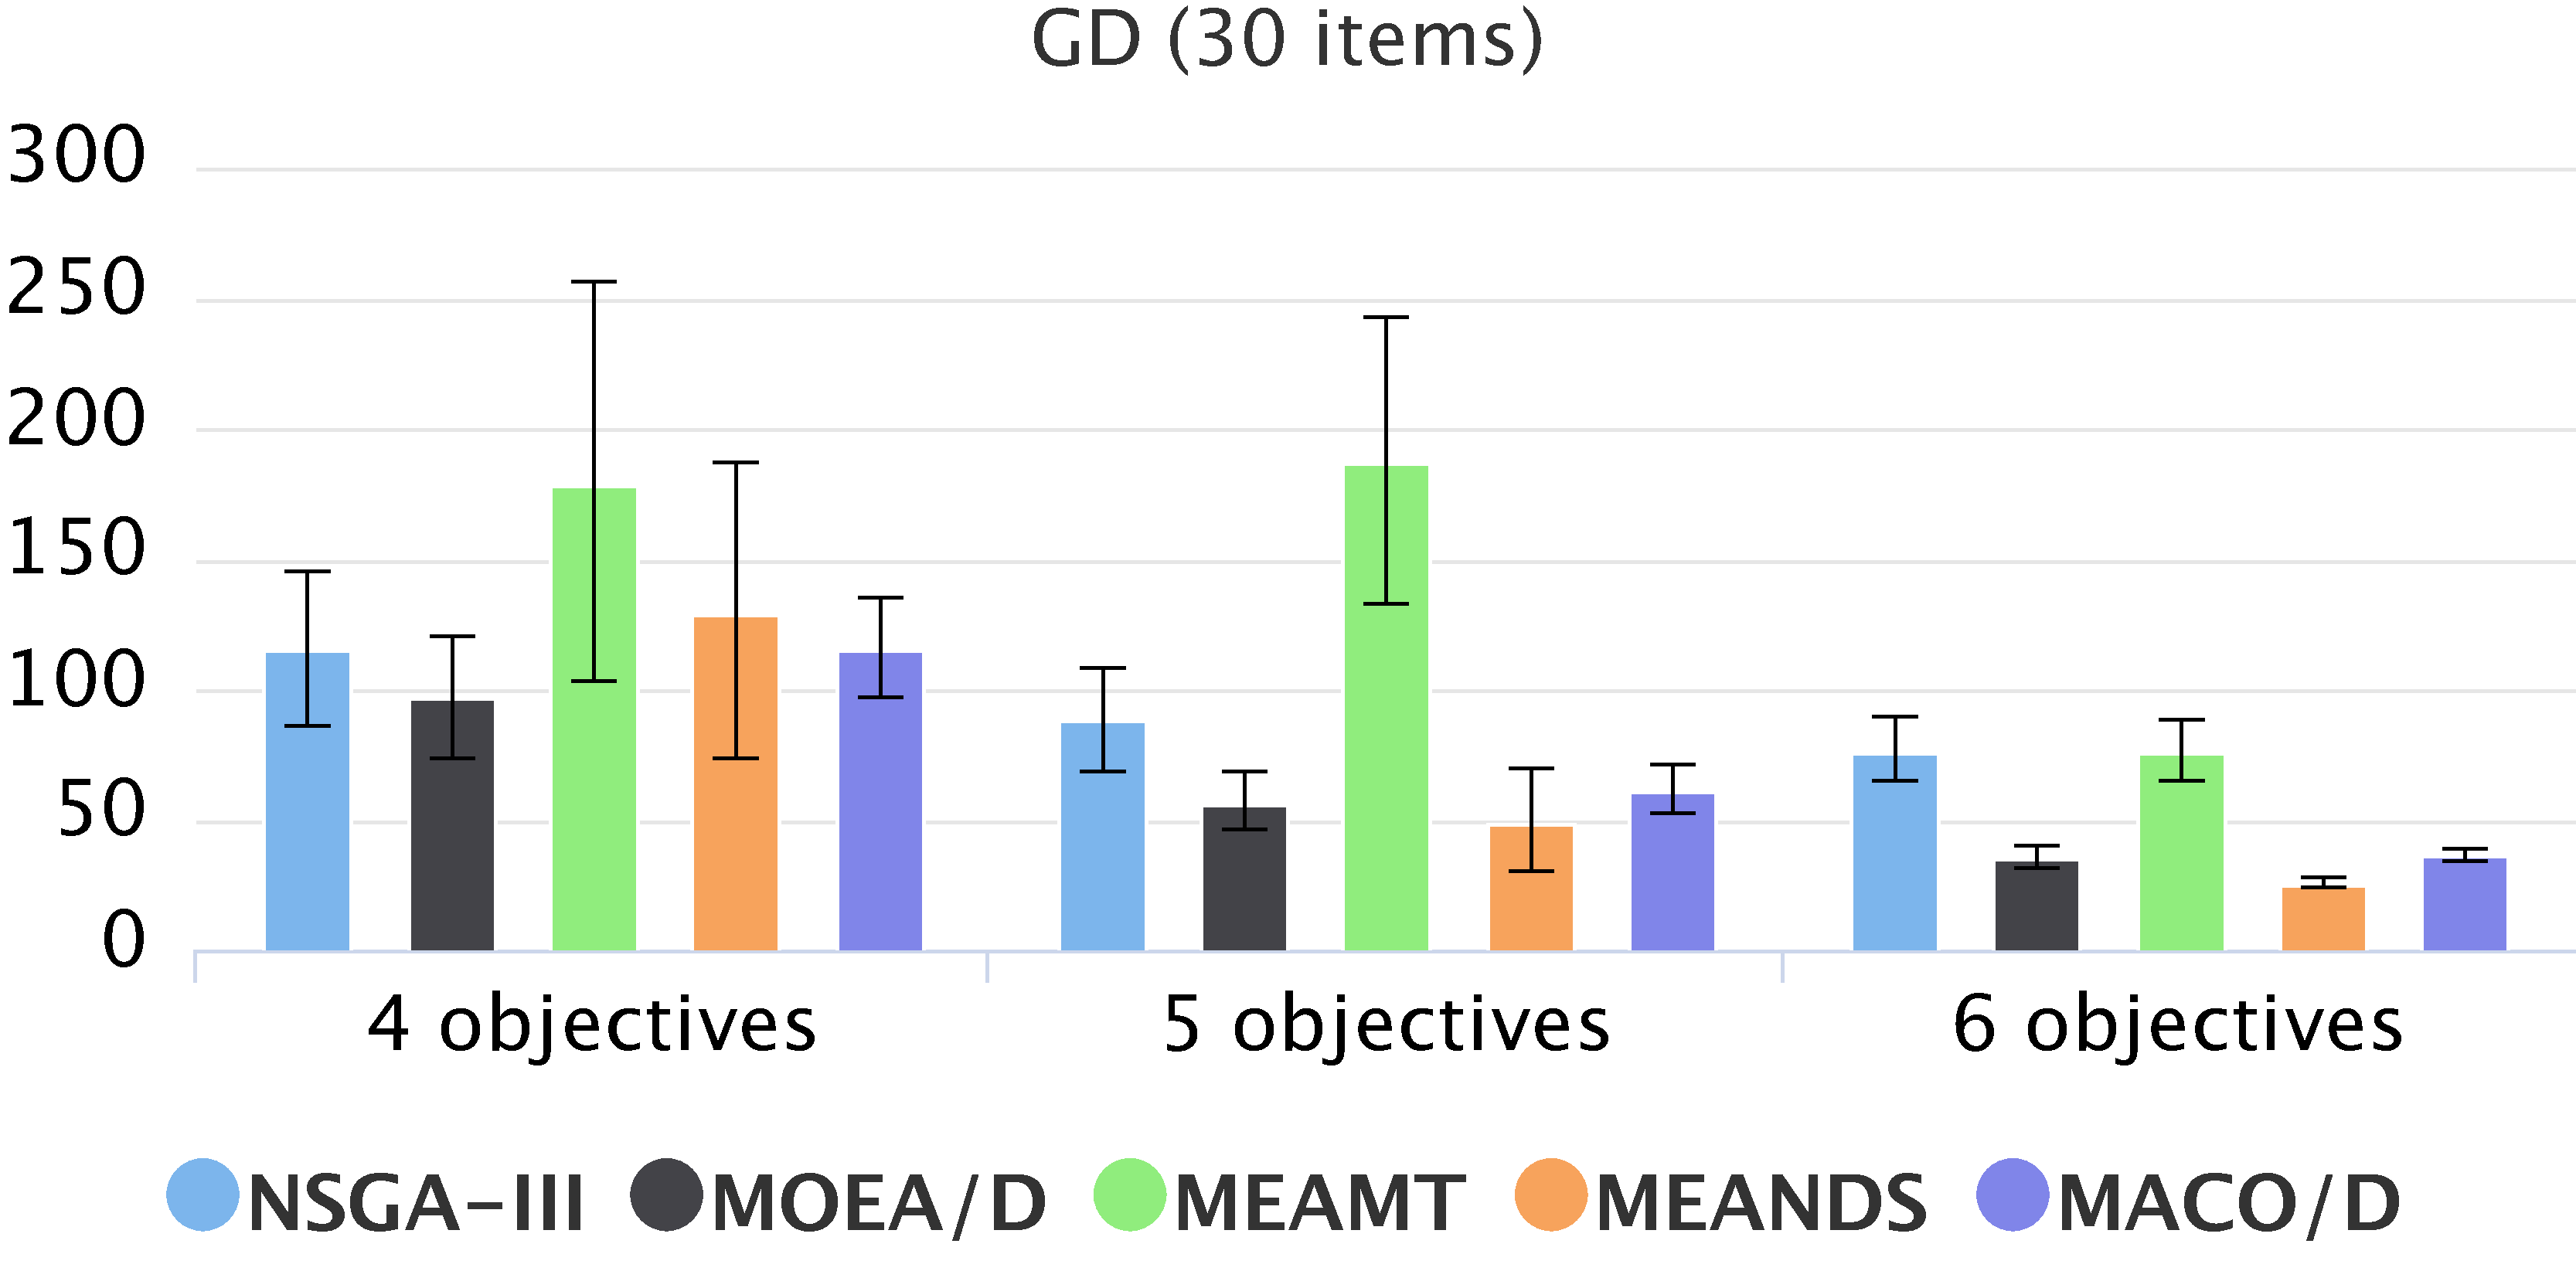
\includegraphics[width=0.5\textwidth]{cap_experimentos/figs/etapa2/gd-mkp-30}
	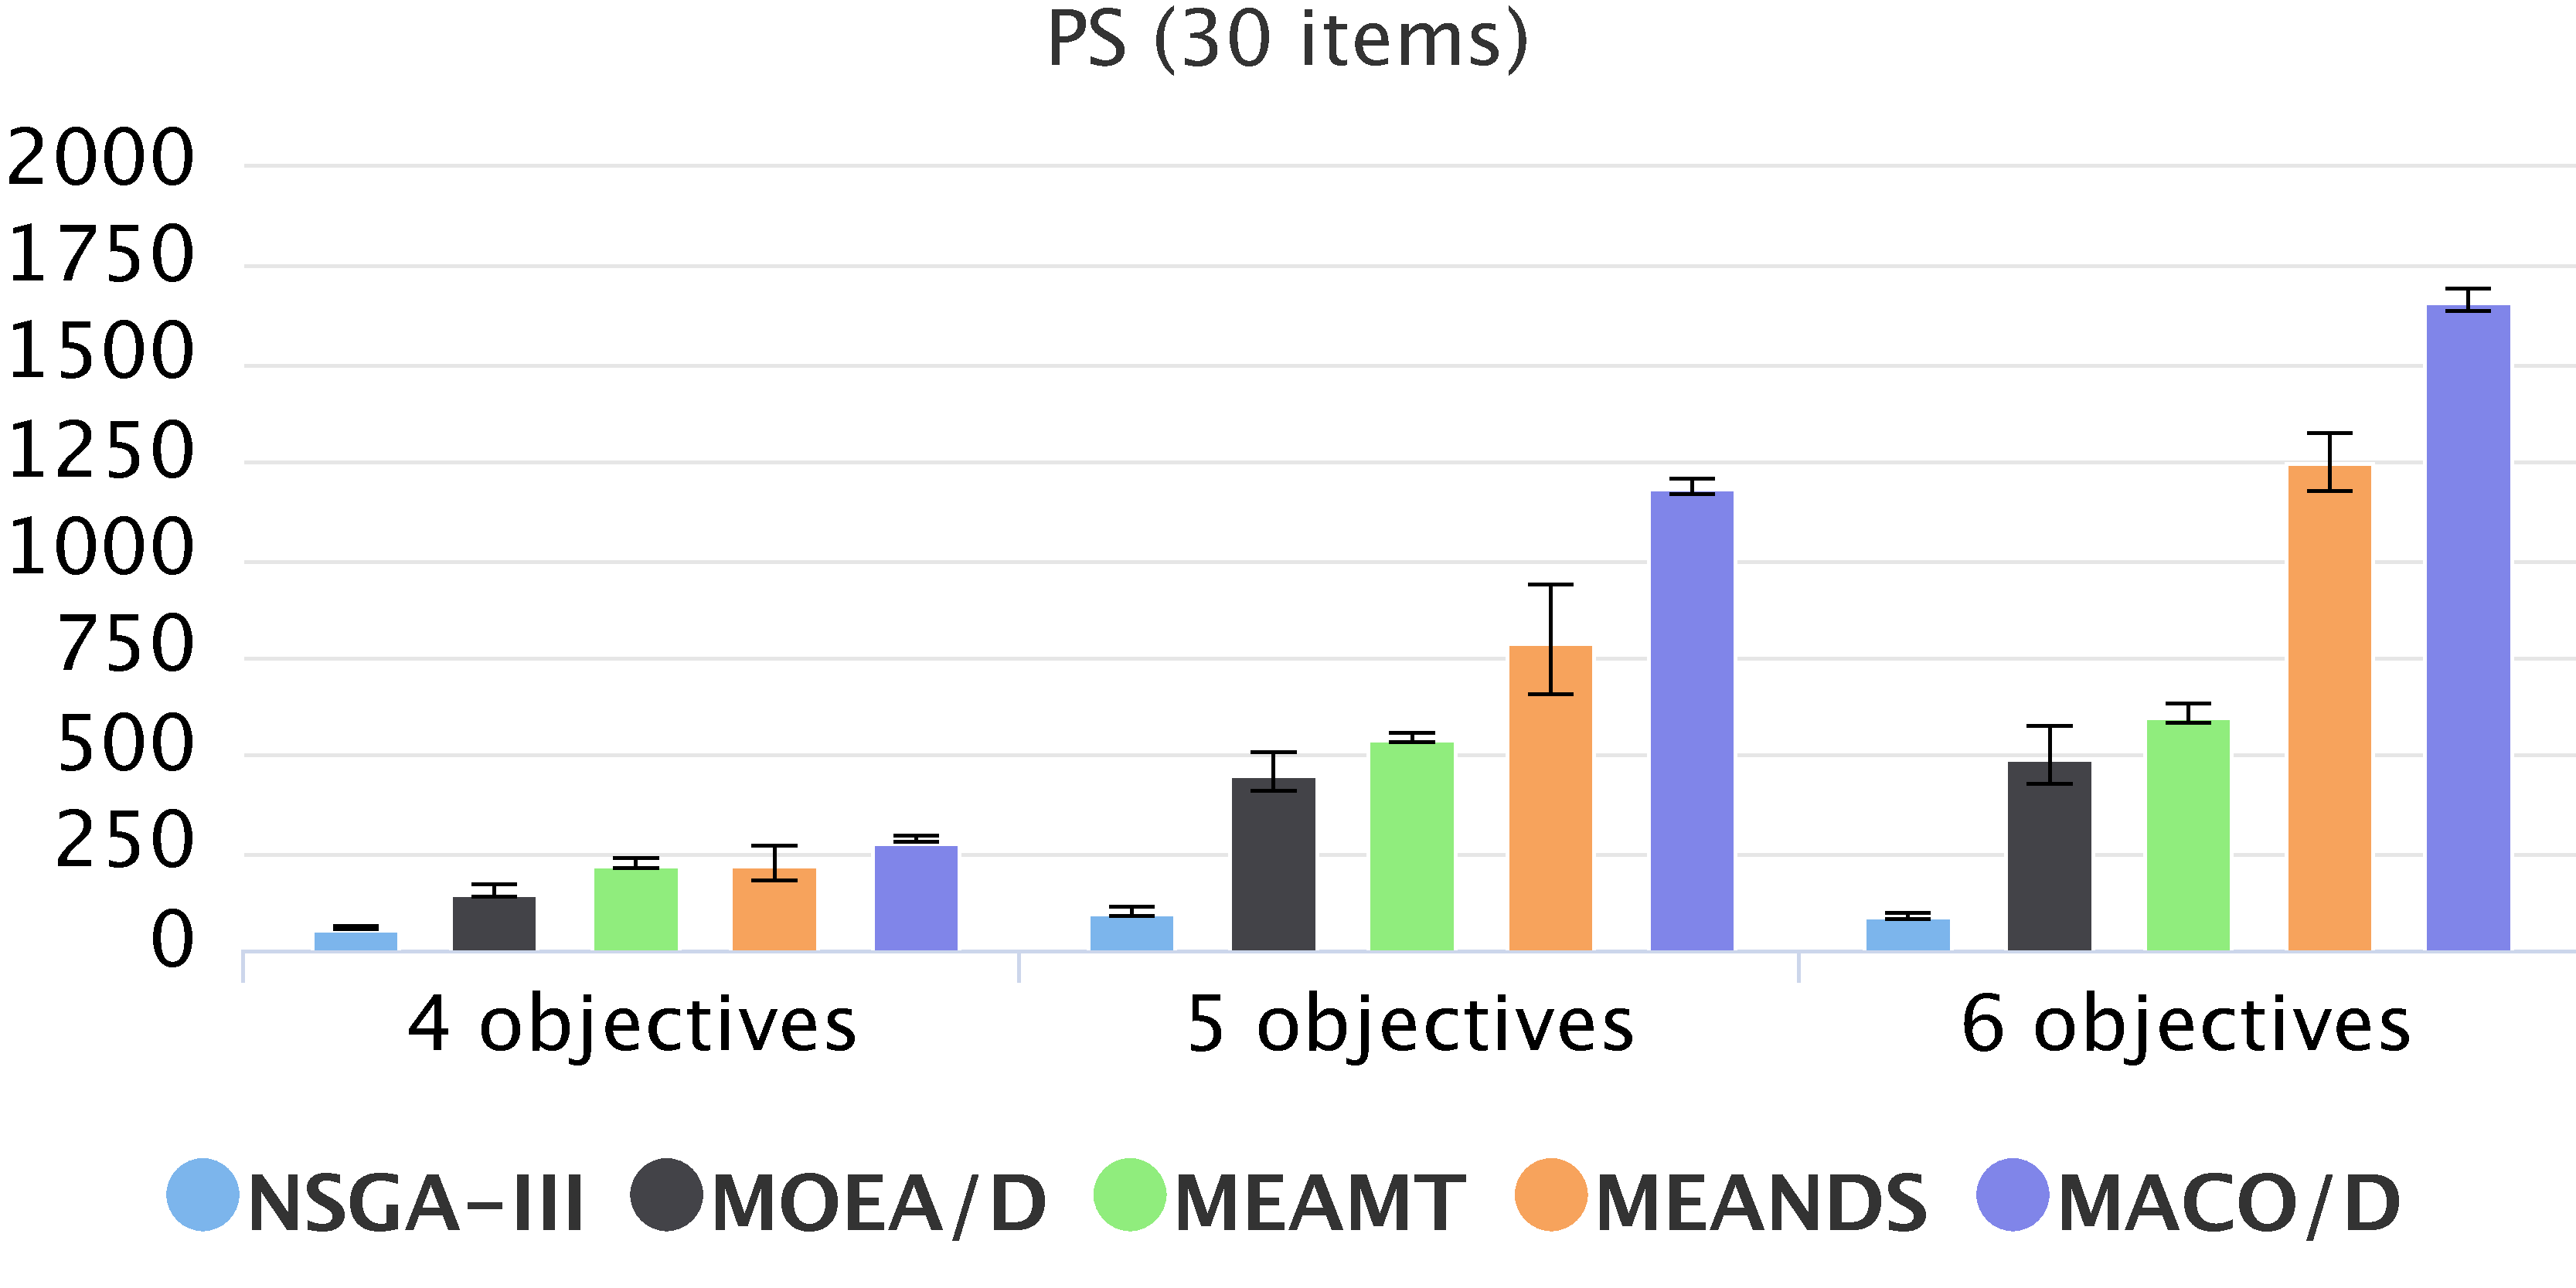
\includegraphics[width=0.5\textwidth]{cap_experimentos/figs/etapa2/ps-mkp-30}
	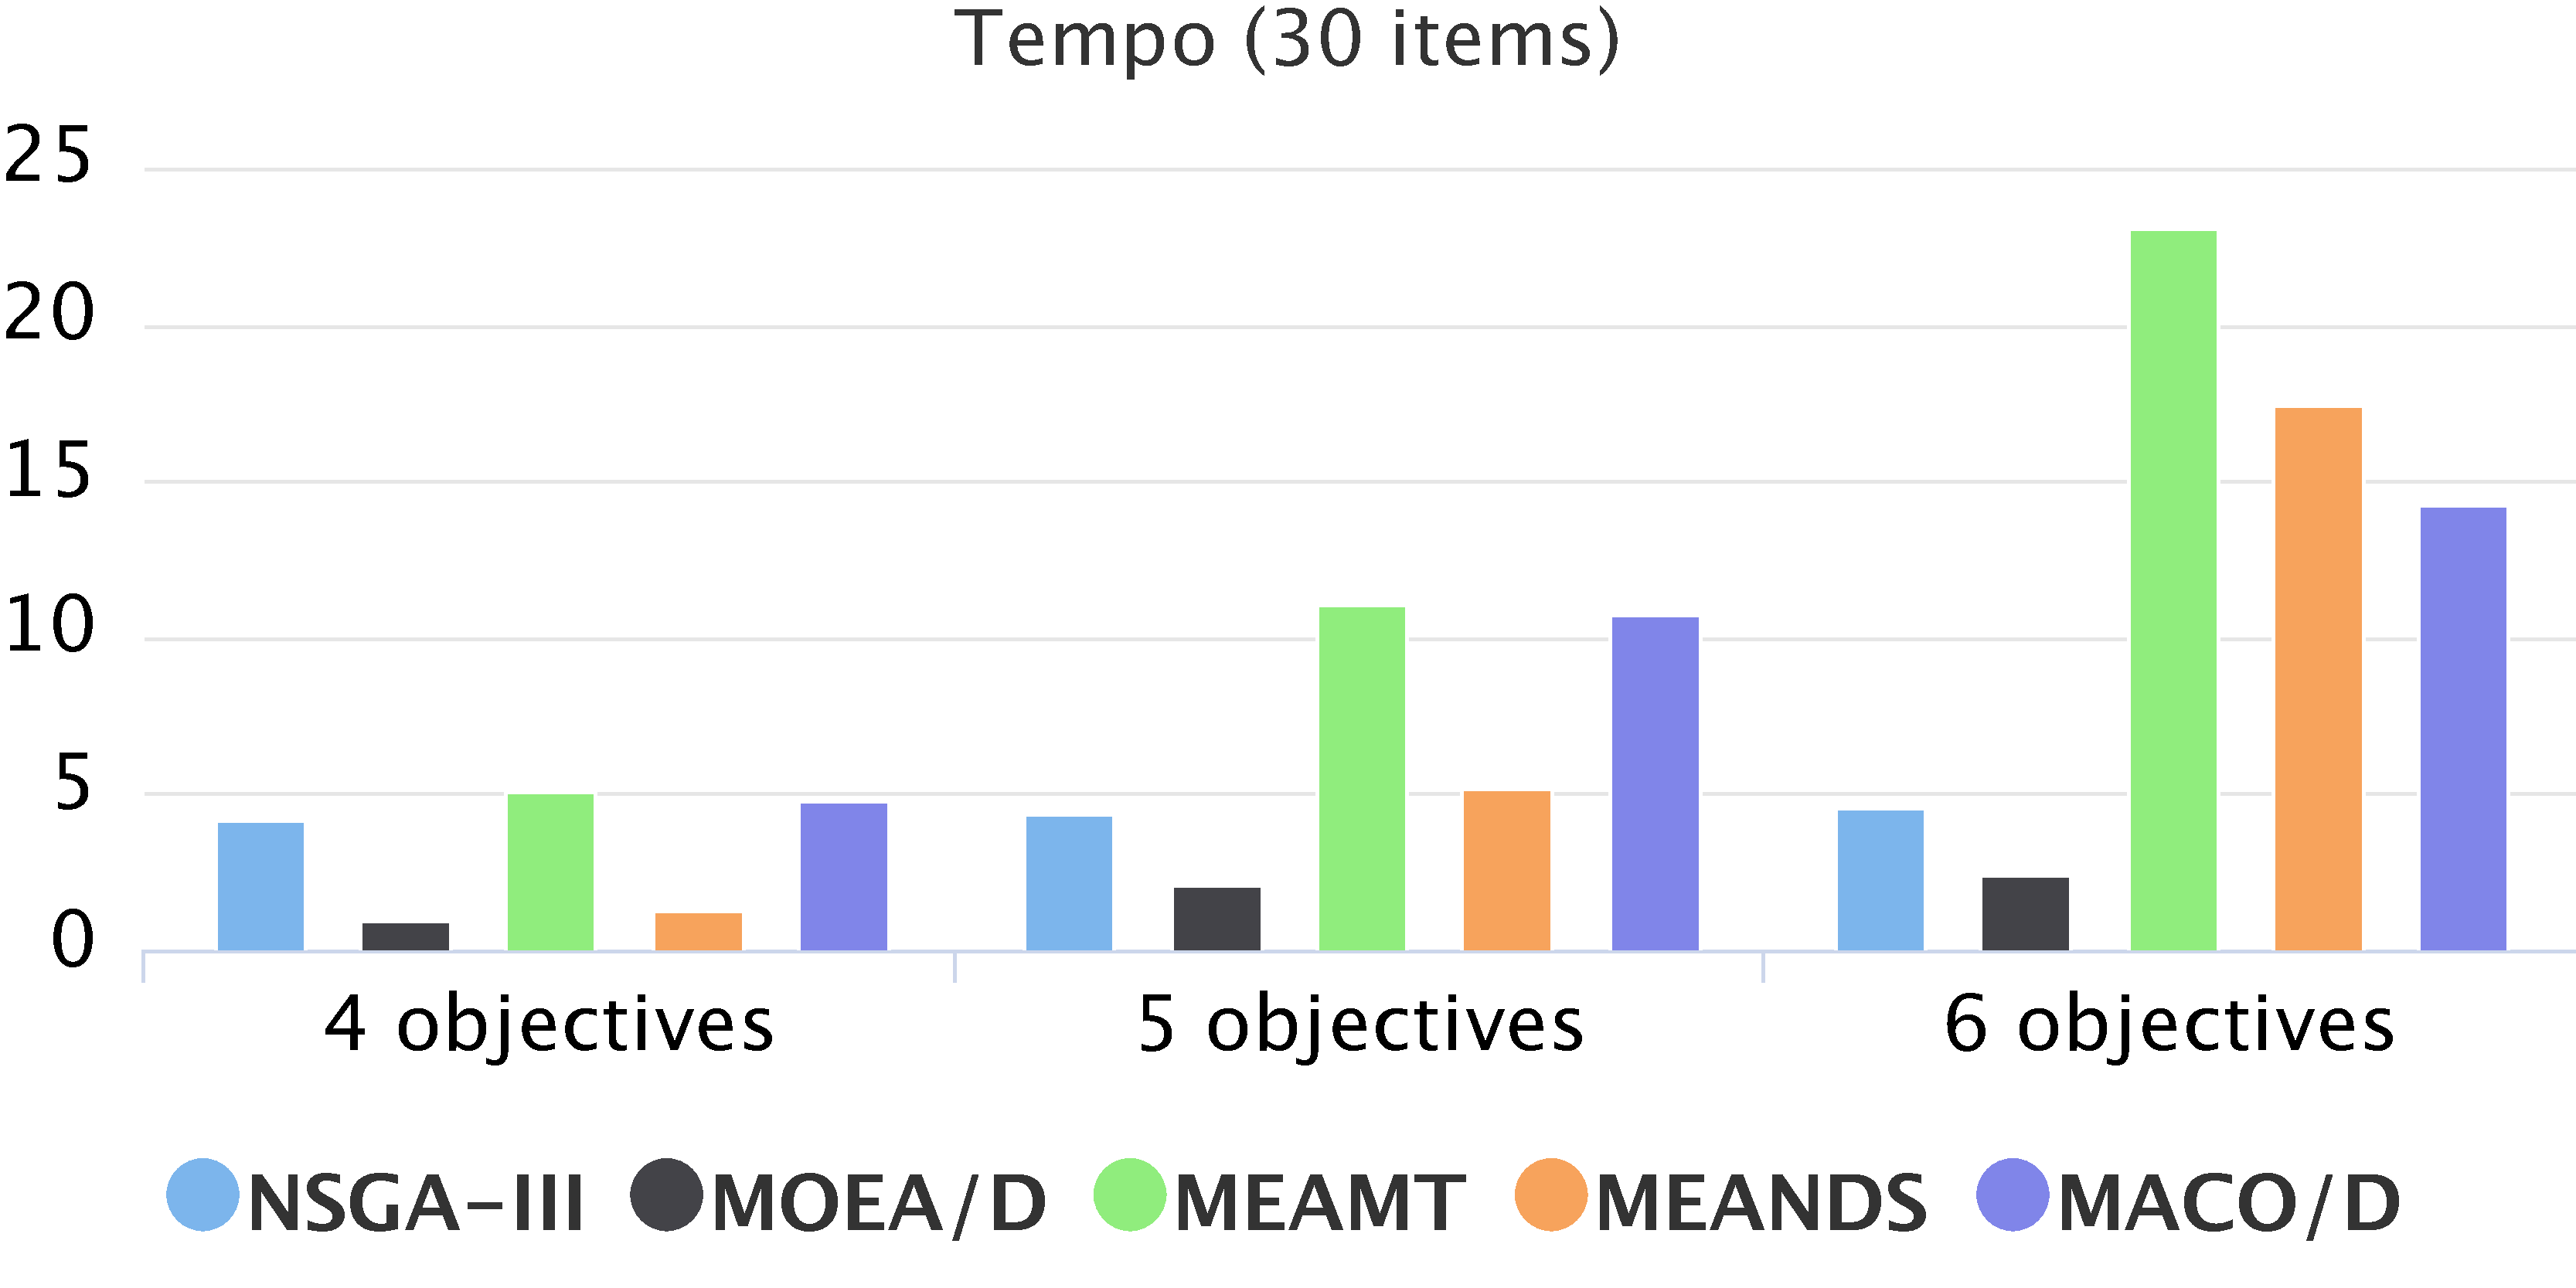
\includegraphics[width=0.5\textwidth]{cap_experimentos/figs/etapa2/time-mkp-30}
\end{figure*}

No problema da mochila mais simples, de 30 itens (figura \ref{fig_exp2_mkp_30}), o AEMMT apresenta a menor taxa de erro dentre os algoritmos \textit{many-objectives}, em segundo lugar está o MACO/D e em terceiro o AEMMD. Com relação ao $GD$, com 4 objetivos, os melhores resultados são encontrados pelo MOEA/D seguido pelo MACO/D. O Em 5 e 6 objetivos, o AEMMD produz o menor $GD$, e o MACO/D, bem próximo, aparece em segundo lugar. Na métrica $PS$, o MACO/D é melhor que os demais em todos as formulações de objetivo, seguido, em ordem pelo AEMMD, AEMMT, MOEA/D e NSGA-III. Destre esses algoritmos, o único com um limite fixo no tamanho do Pareto é o NSGA-III, portanto, é esperado que possua um valor de $PS$ menor. Quanto ao tempo, o MOEA/D é o algoritmo mais rápido dentre os 5.

\begin{figure*}[!htbp]
	\caption{Etapa 2: resultados para o PMM com 40 itens}
	\label{fig_exp2_mkp_50}
	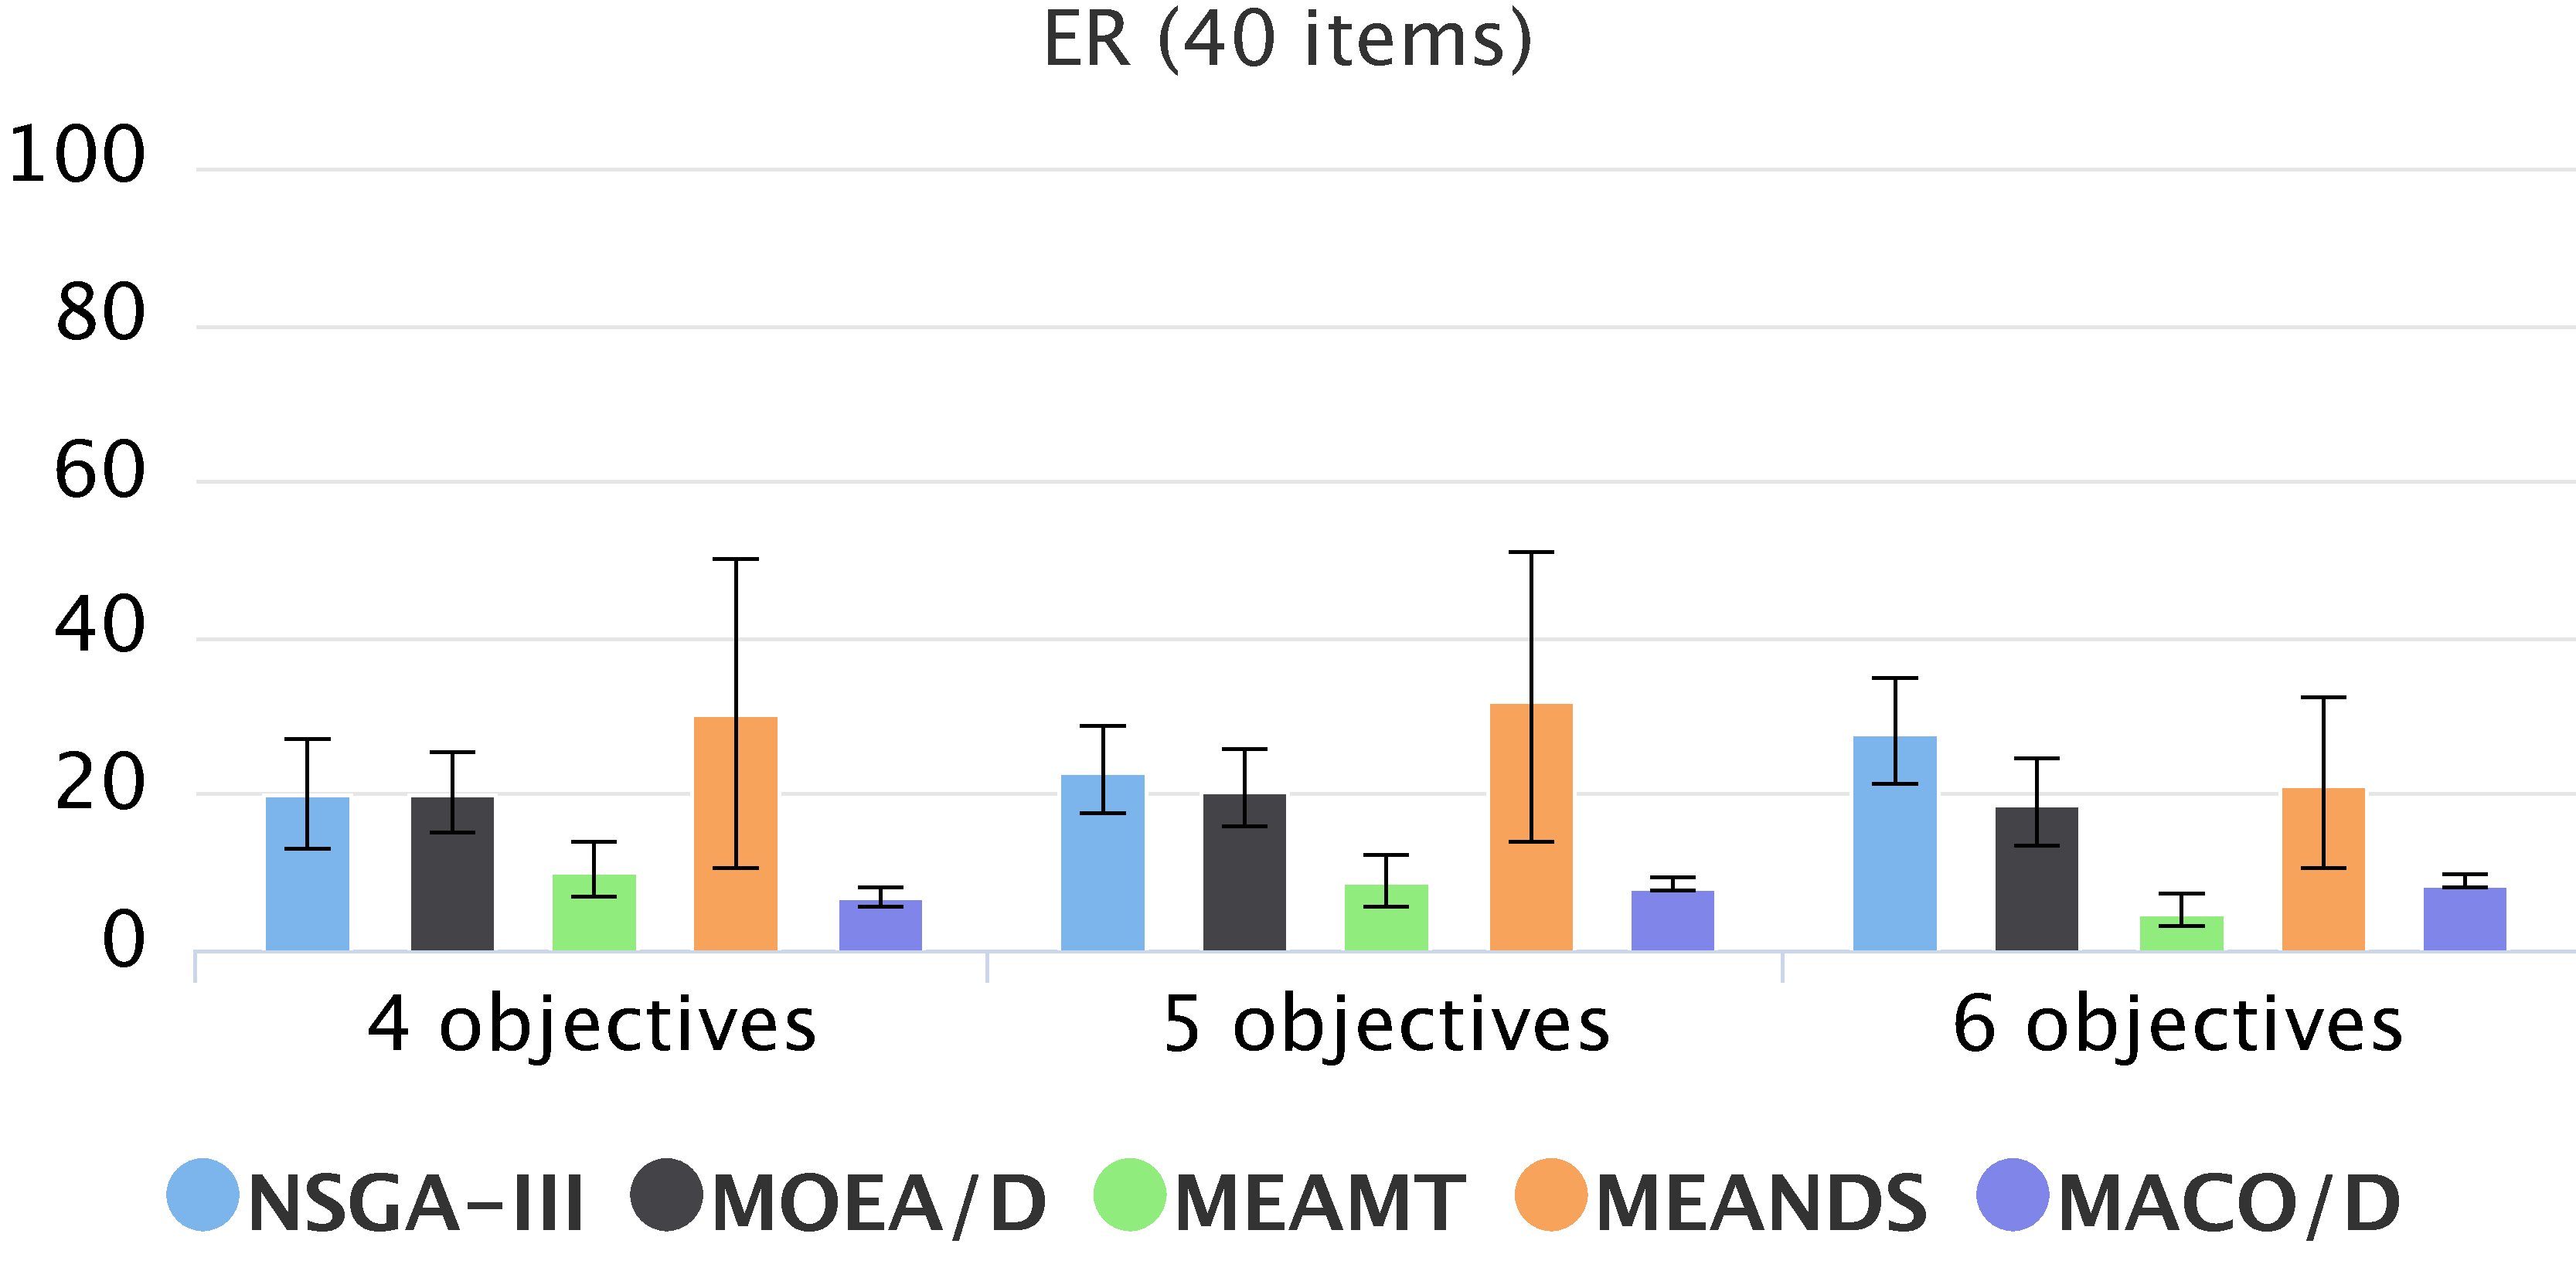
\includegraphics[width=0.5\textwidth]{cap_experimentos/figs/etapa2/er-mkp-40}
	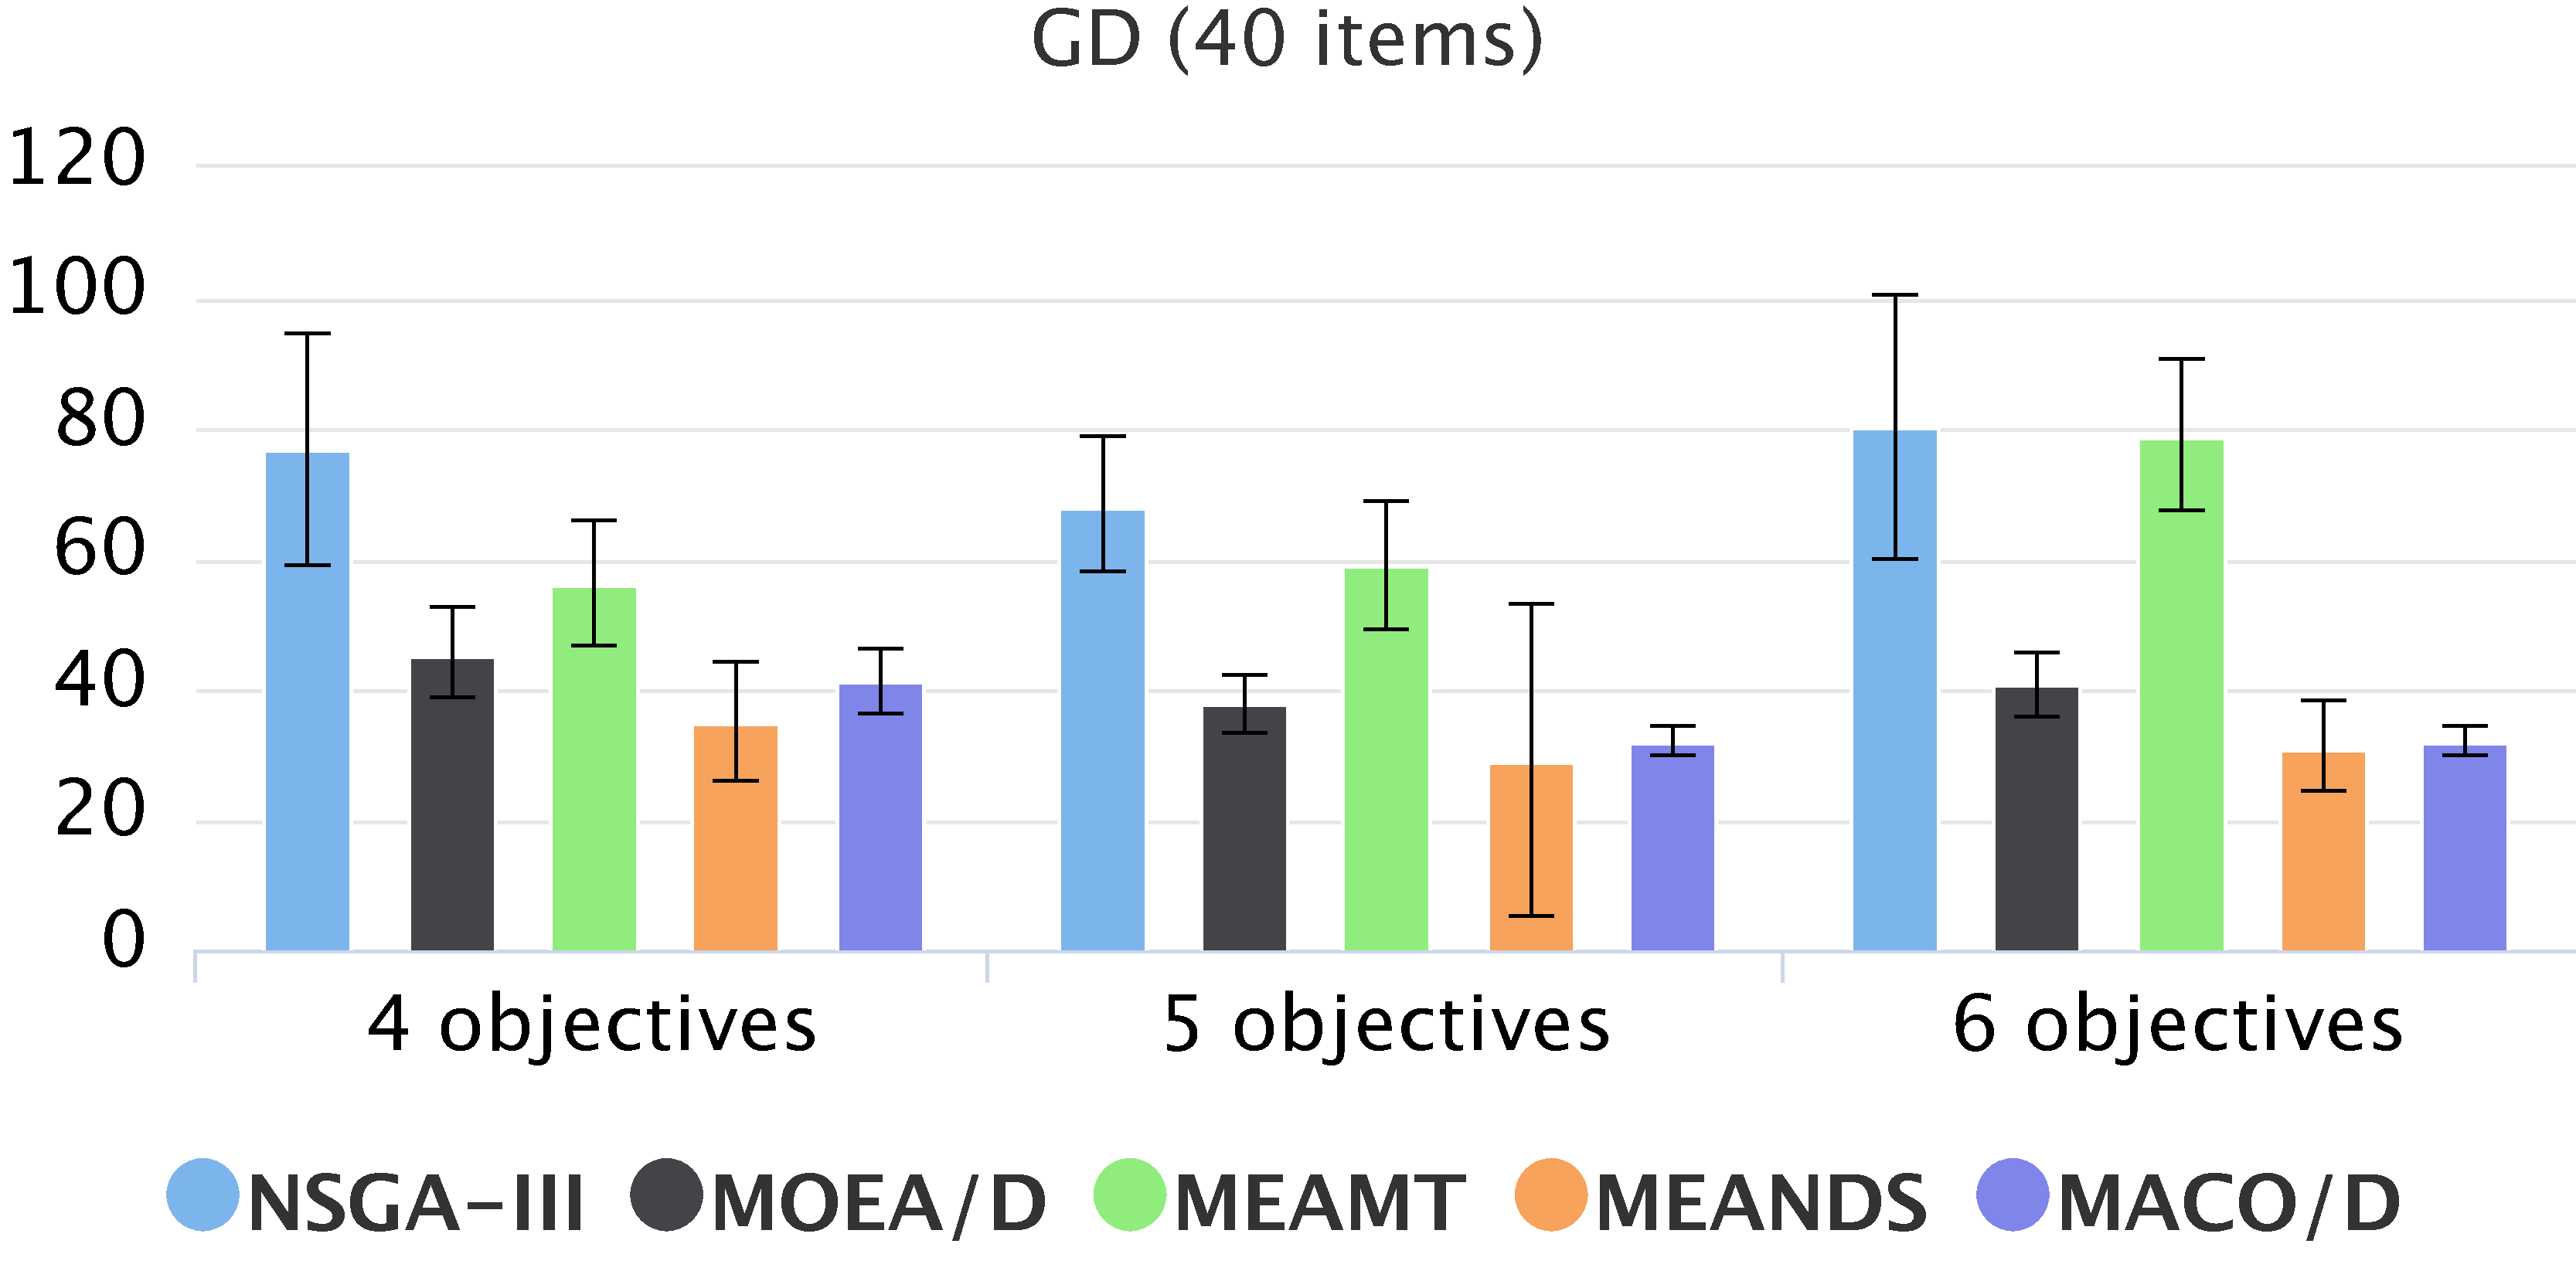
\includegraphics[width=0.5\textwidth]{cap_experimentos/figs/etapa2/gd-mkp-40}
	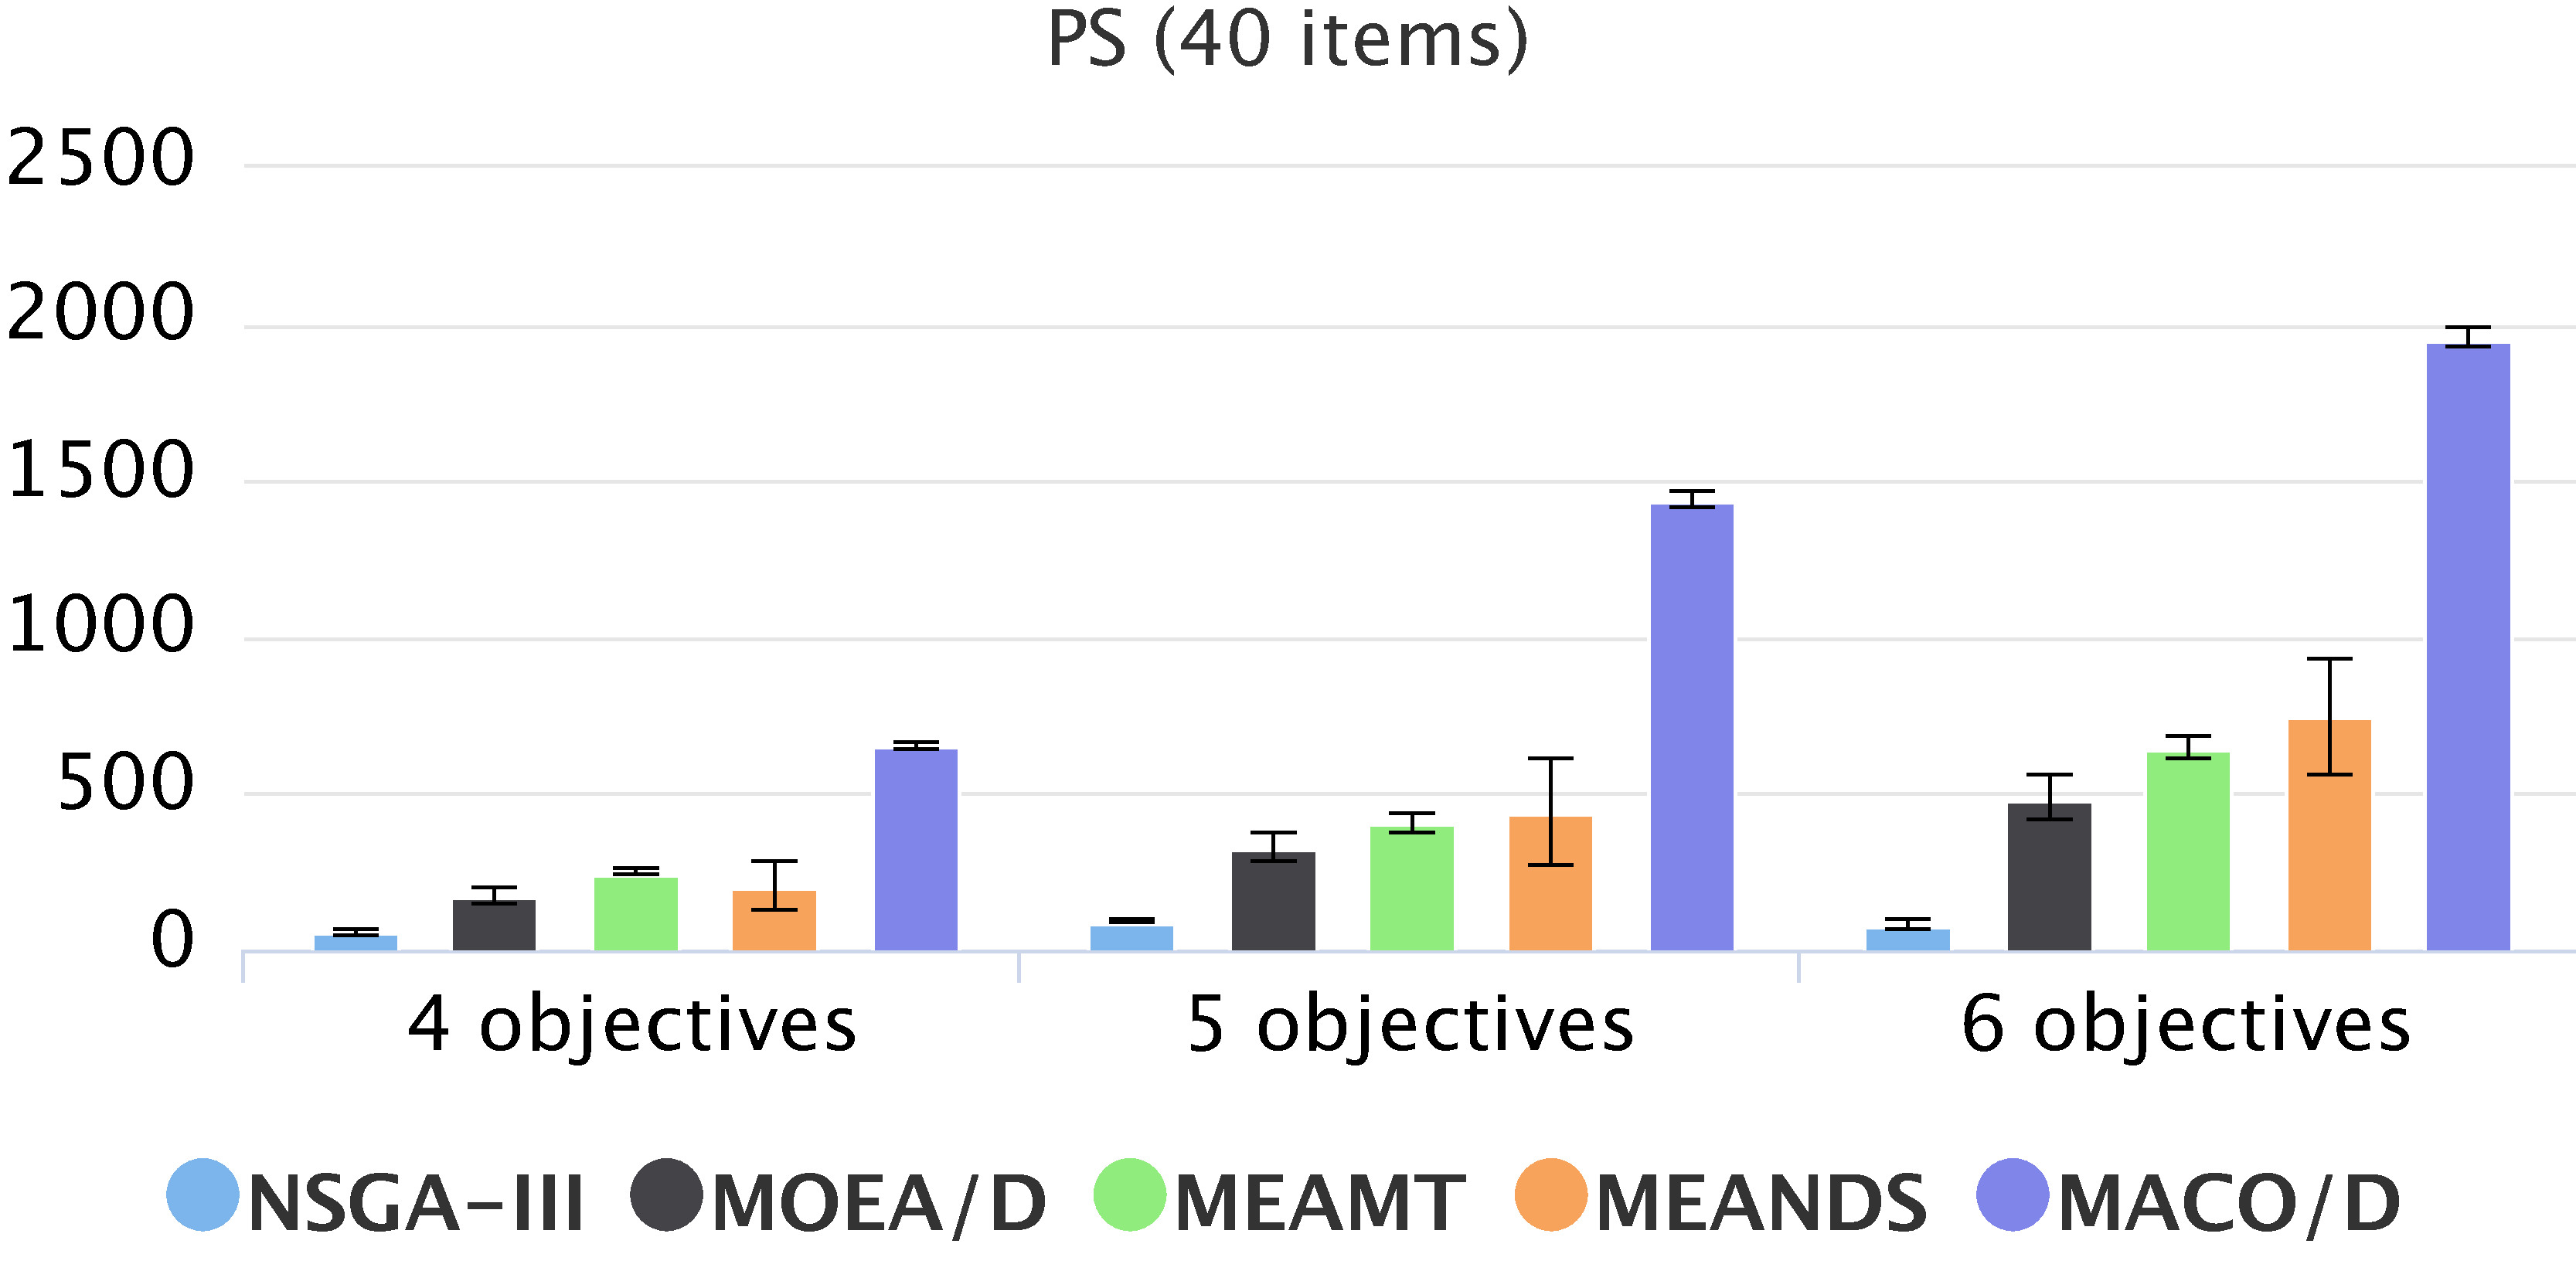
\includegraphics[width=0.5\textwidth]{cap_experimentos/figs/etapa2/ps-mkp-40}
	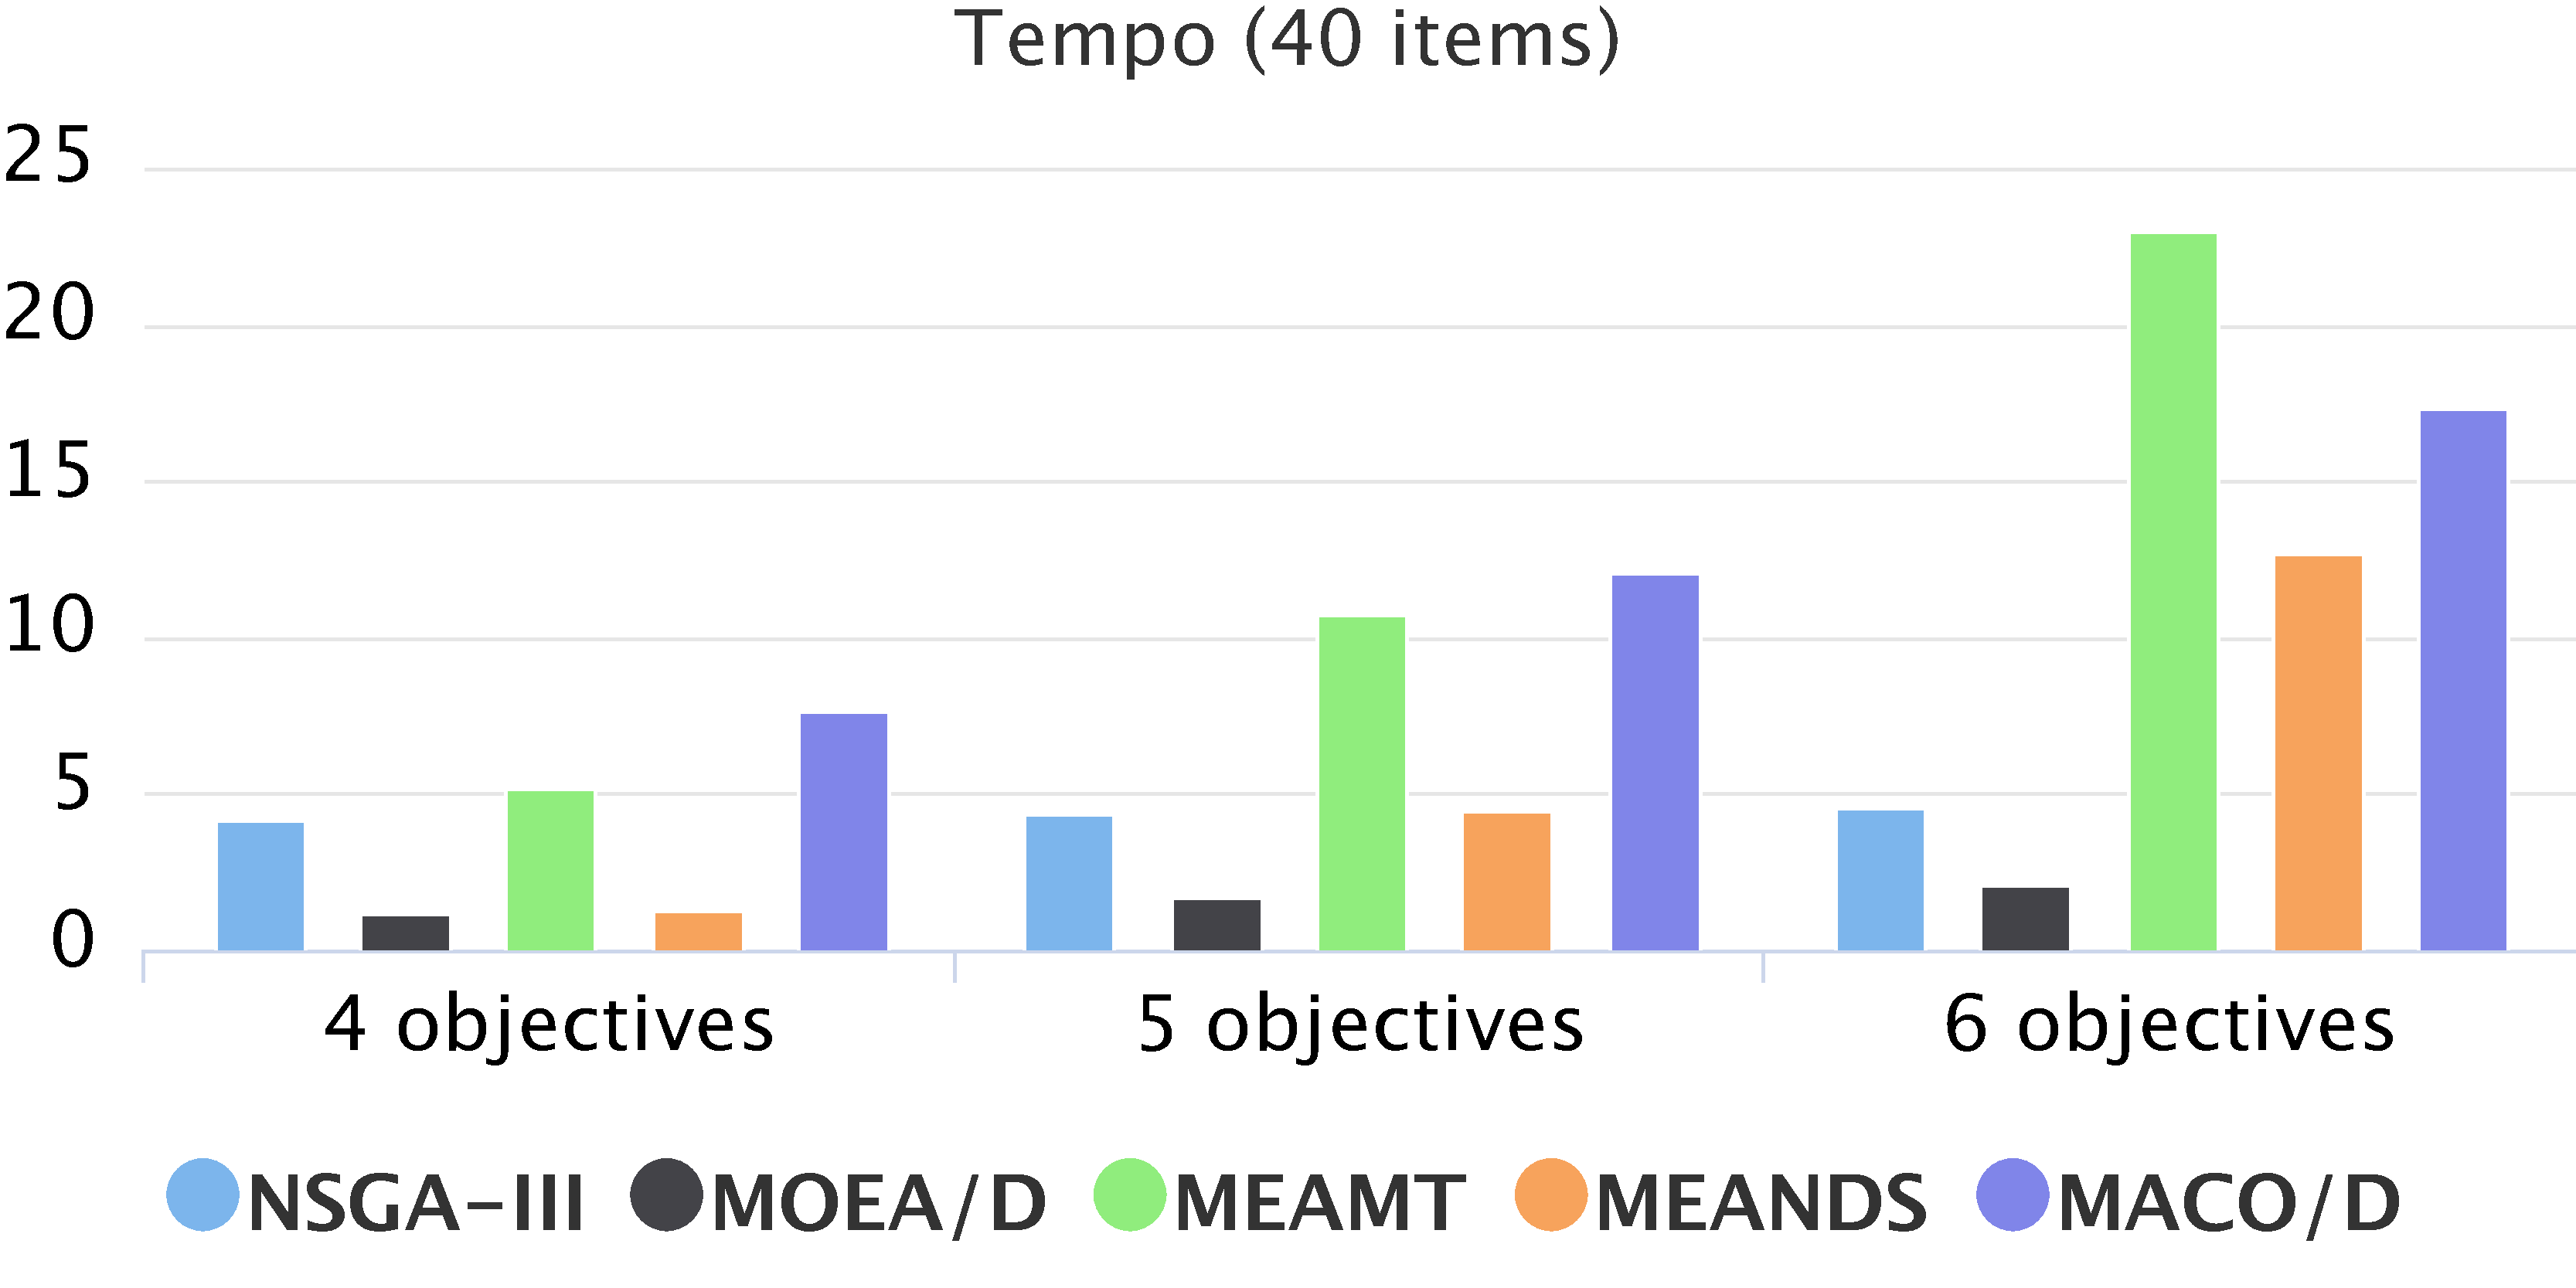
\includegraphics[width=0.5\textwidth]{cap_experimentos/figs/etapa2/time-mkp-40}
\end{figure*}

O PMM de 40 itens é analisado na figura \ref{fig_exp2_mkp_40}. O AEMMT e o MACO/D apresentam a menor taxa de erro, sendo que o MACO/D é melhor para 4 e 5 objetivos, enquanto o AEMMT obtém o melhor resultado para 6 objetivos. Os melhores valores de $GD$ foram encontrados pelo AEMMD e MACO/D, sendo que o AEMMD é um pouco melhor no problema com 4 objetivos. Uma característica negativa do AEMMD em relação ao MACO/D no que se refere ao $GD$ é sua alta variação nos resultados, o que diz que algumas execuções produz soluções muito próximas do Pareto enquanto outras nem tanto. A respeito do tamanho dos Paretos encontrados, novamente o MACO/D lidera independente da formulação de objetivos. O MOEA/D é o algoritmo mais rápido, enquanto o AEMMT e o MACO/D são os mais lentos.

\begin{figure*}[!htbp]
	\caption{Etapa 2: resultados para o PMM com 50 itens}
	\label{fig_exp2_mkp_100}
	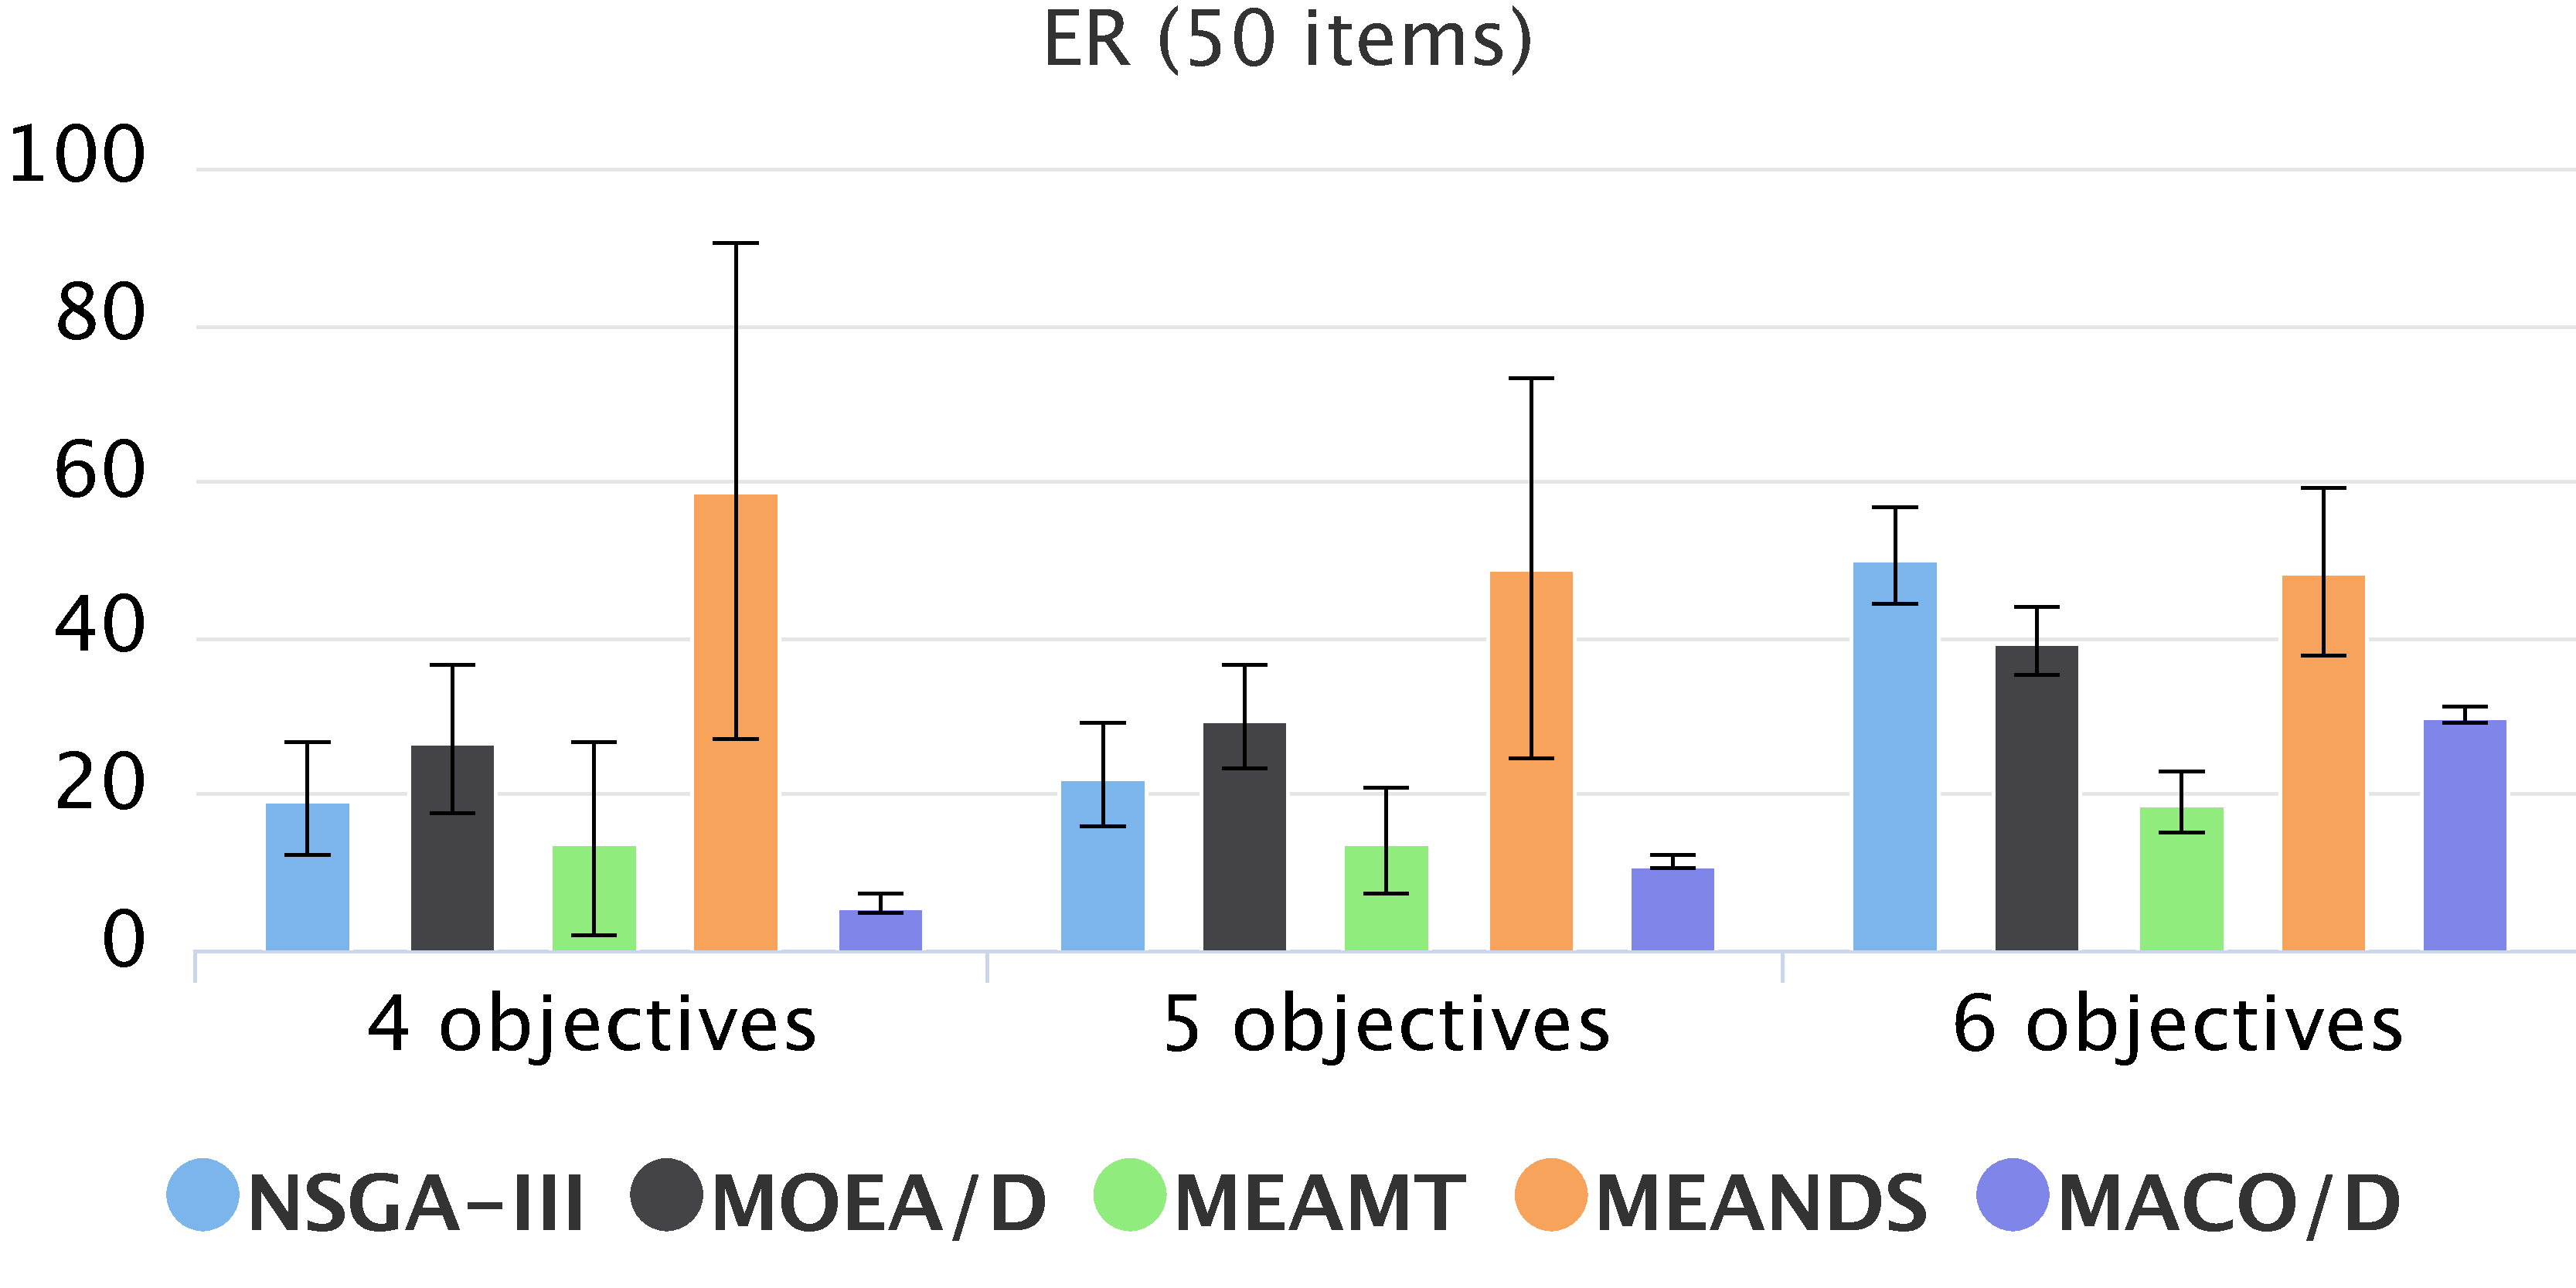
\includegraphics[width=0.5\textwidth]{cap_experimentos/figs/etapa2/er-mkp-50}
	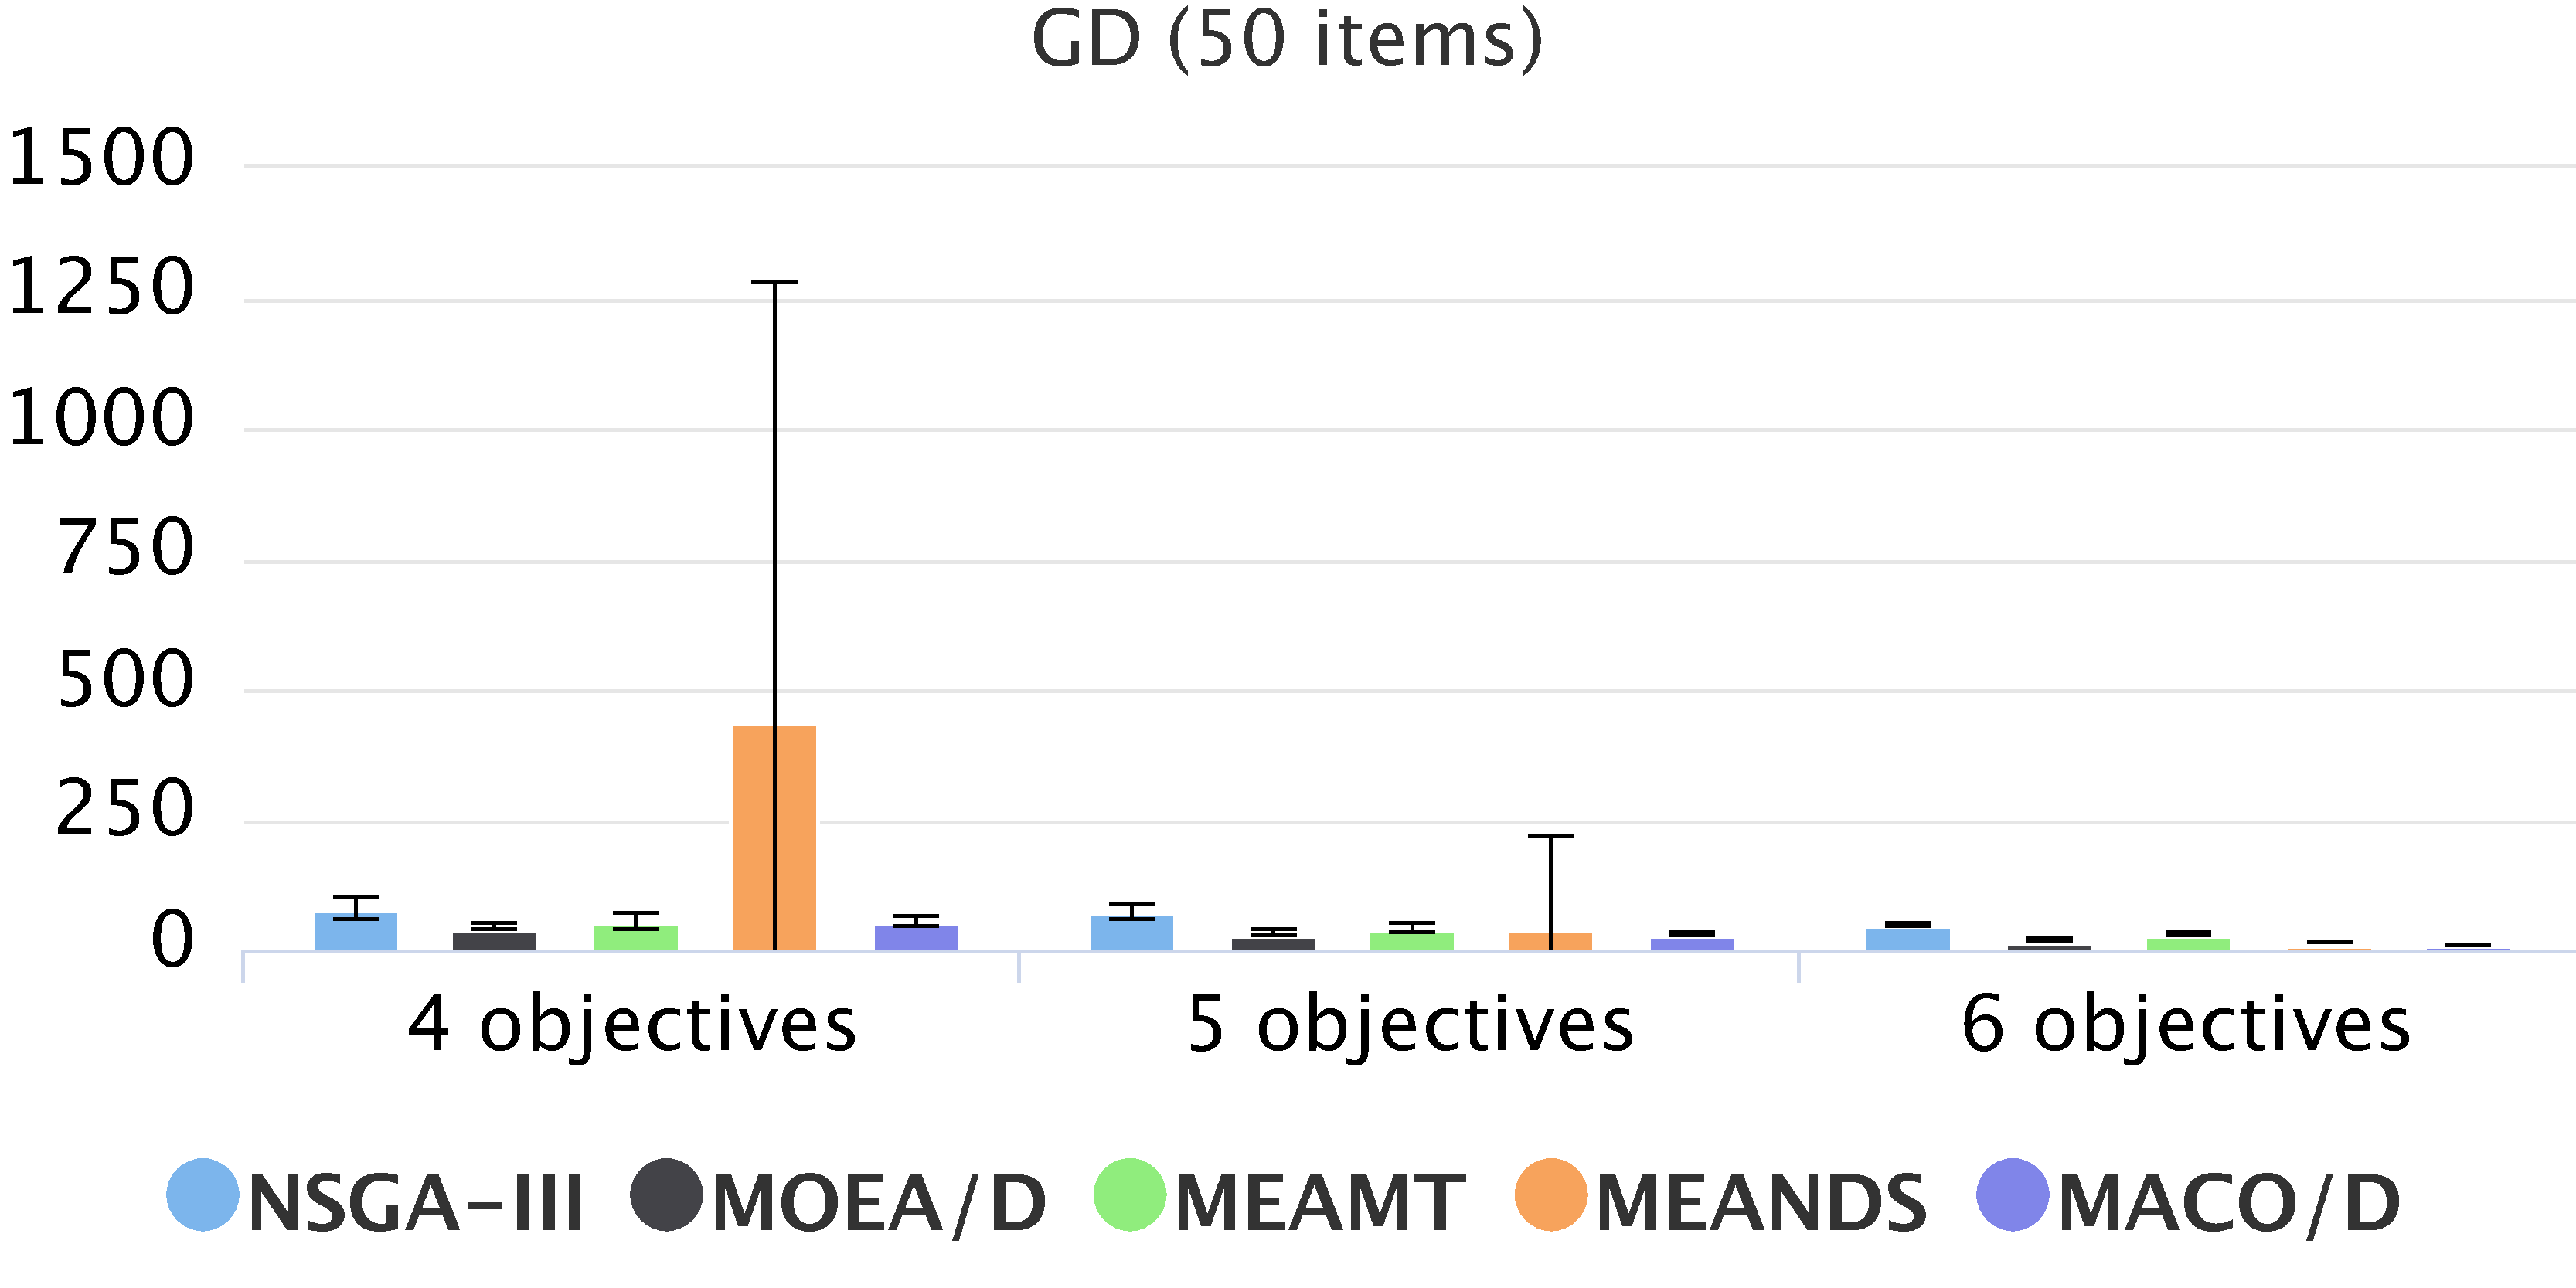
\includegraphics[width=0.5\textwidth]{cap_experimentos/figs/etapa2/gd-mkp-50}
	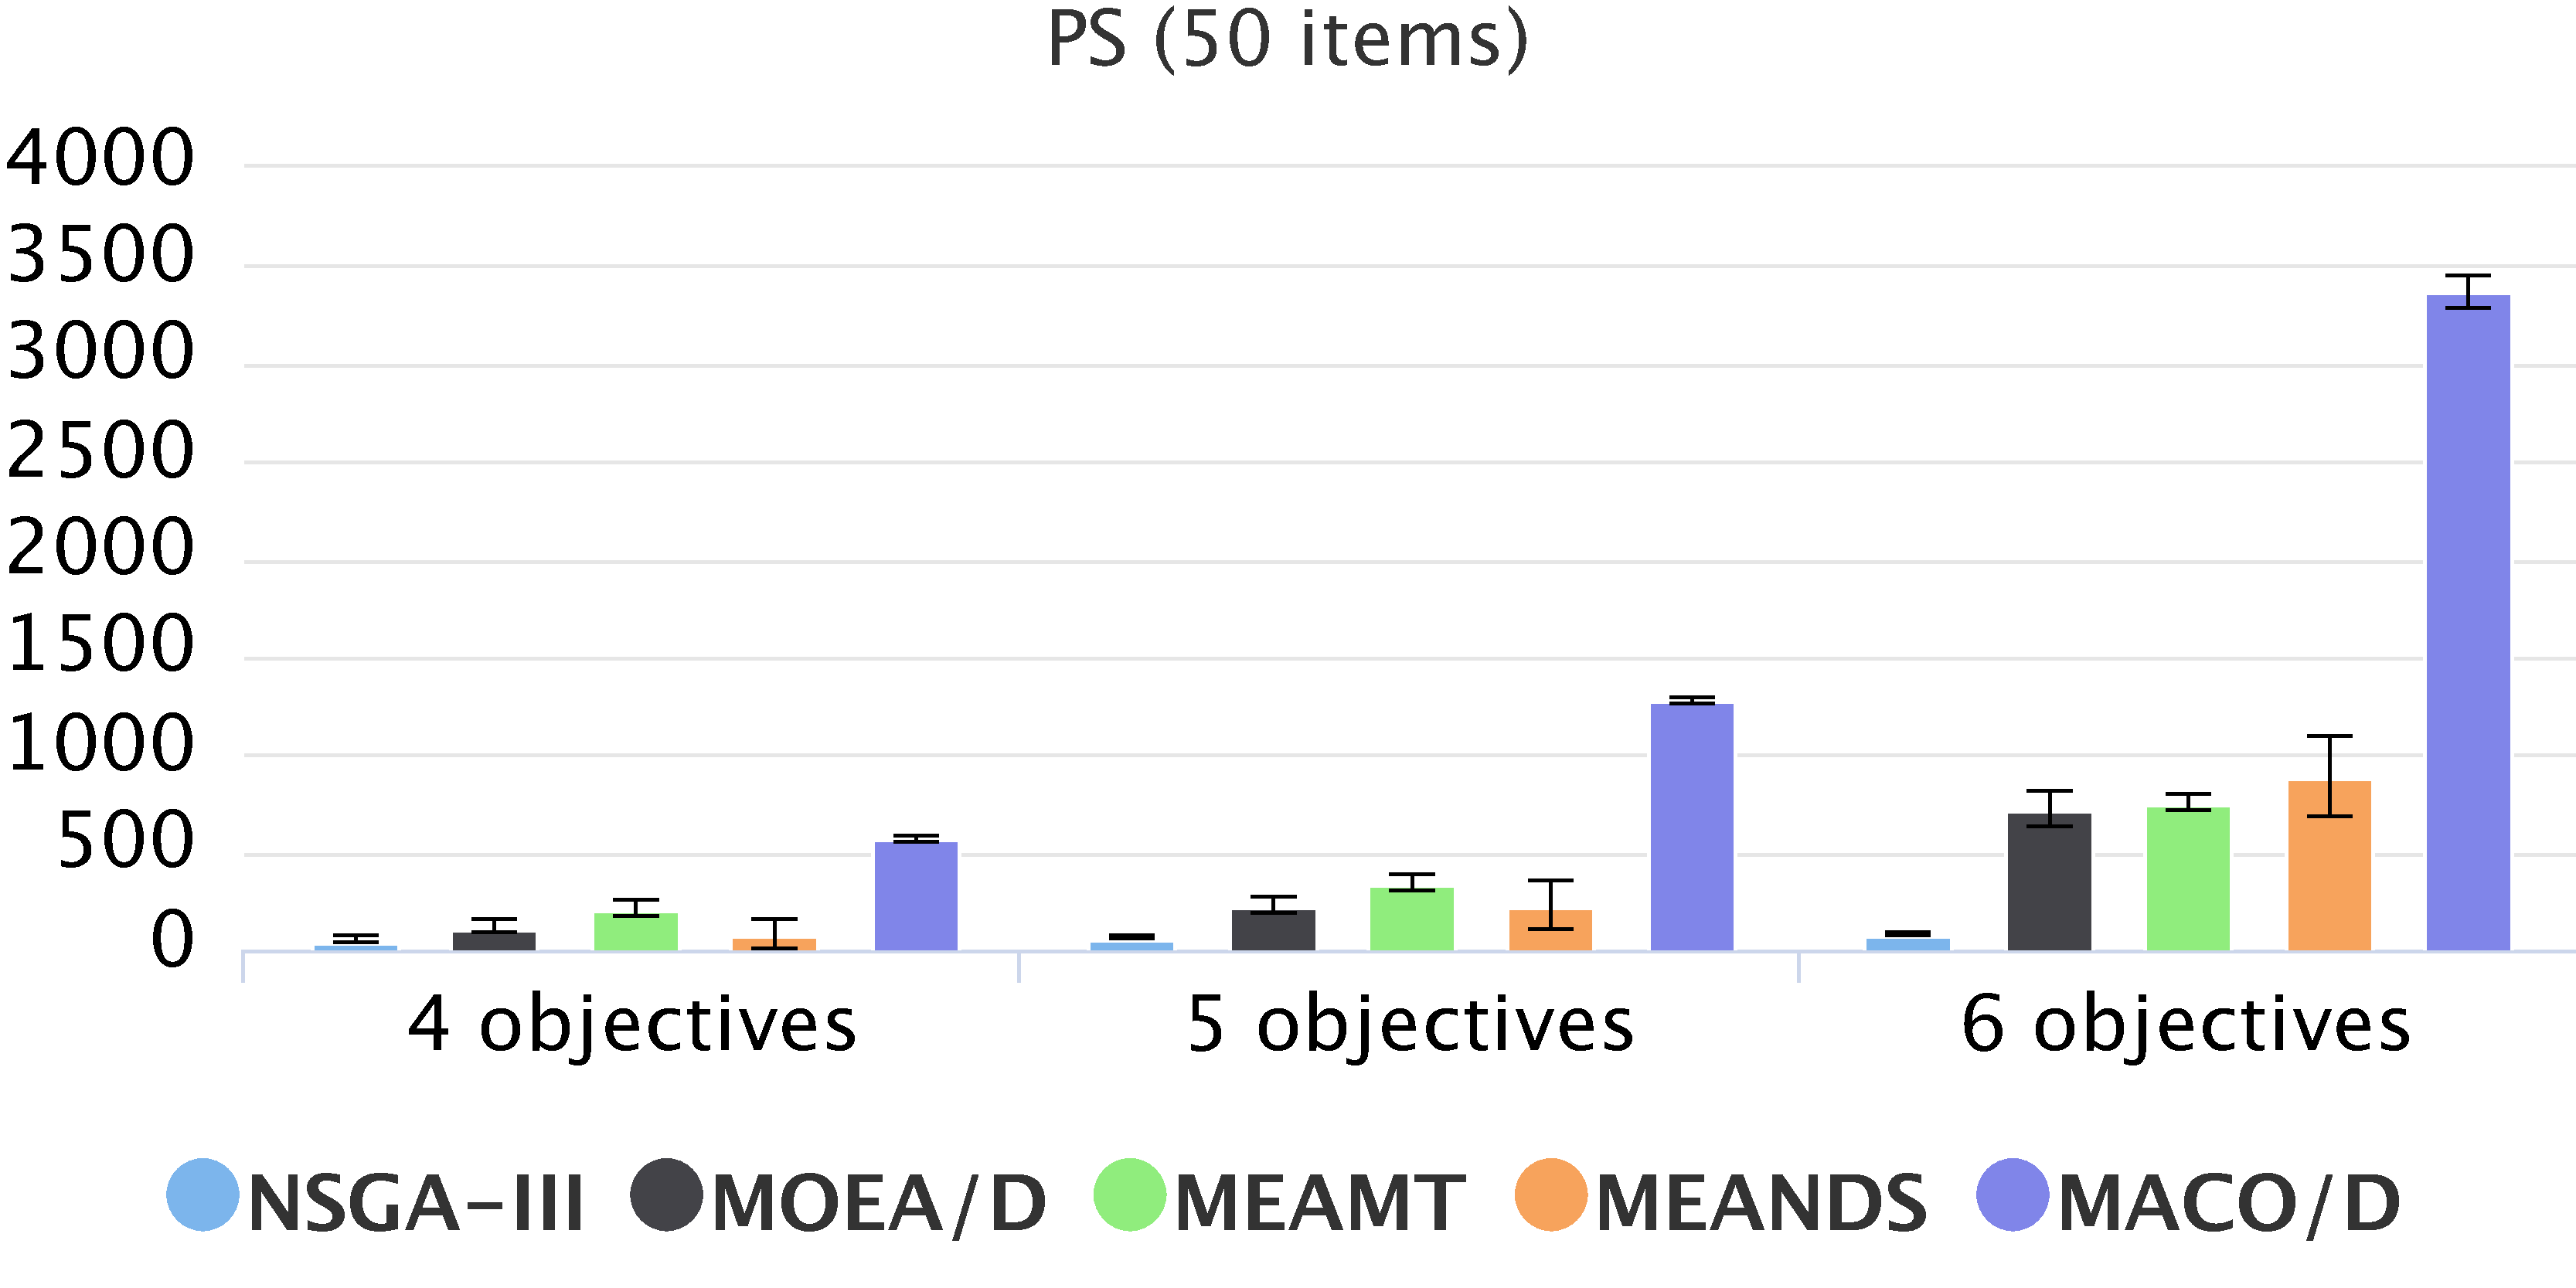
\includegraphics[width=0.5\textwidth]{cap_experimentos/figs/etapa2/ps-mkp-50}
	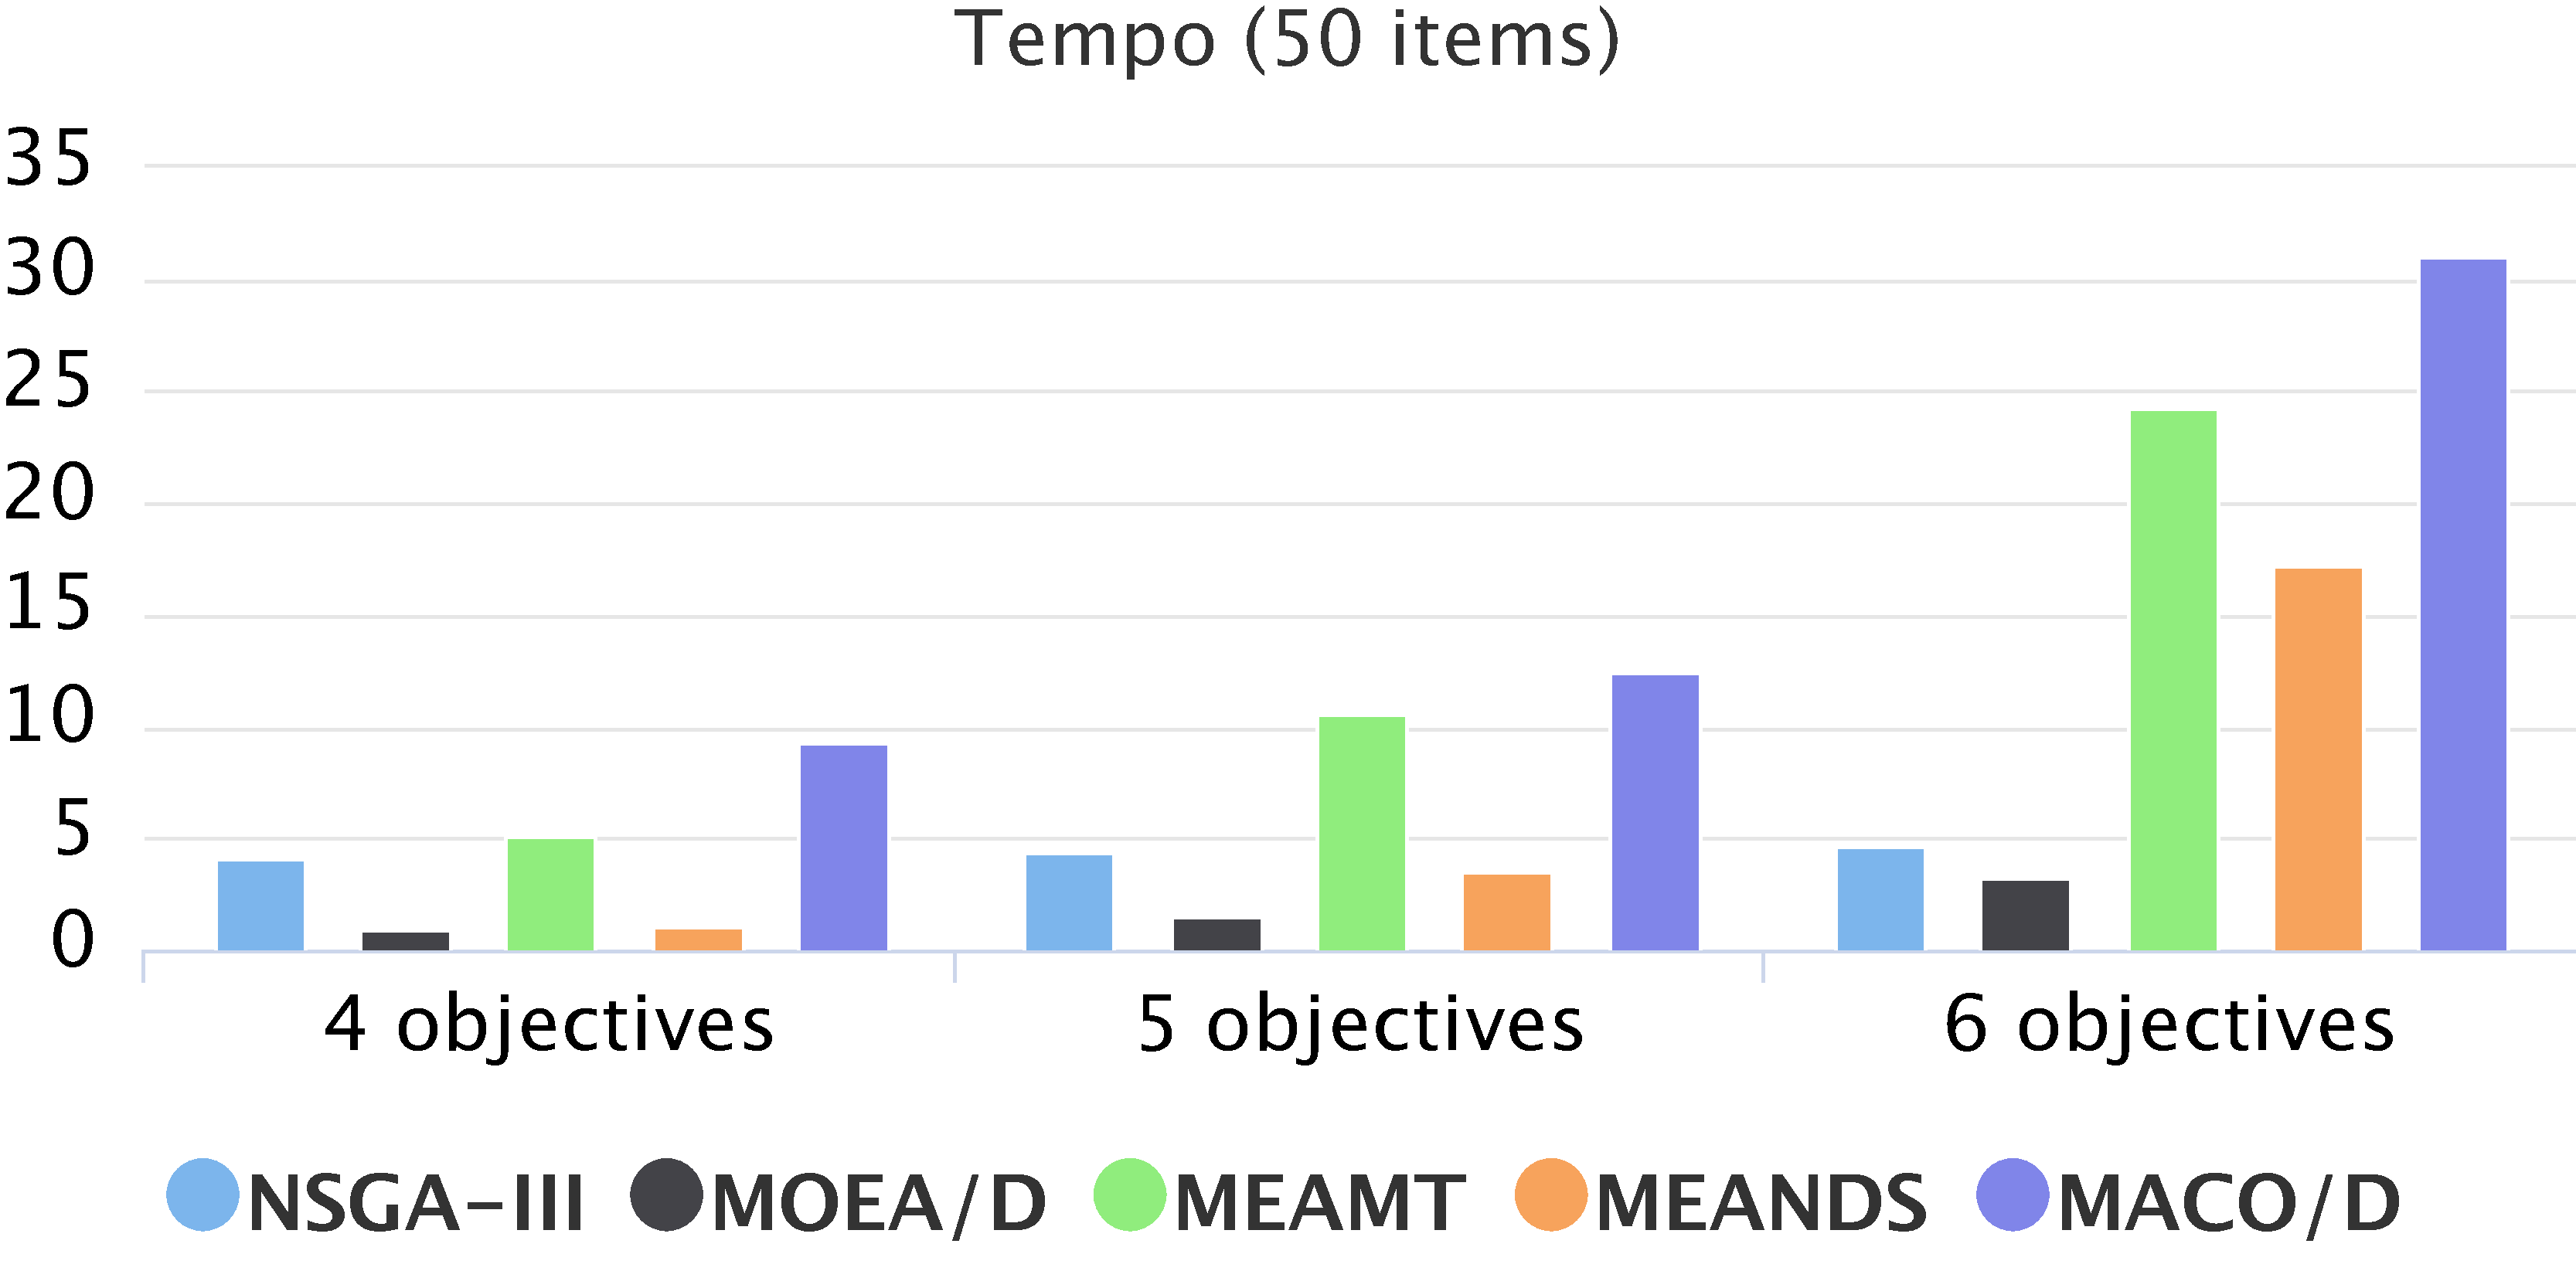
\includegraphics[width=0.5\textwidth]{cap_experimentos/figs/etapa2/time-mkp-50}
\end{figure*}

O PMM com 50 itens (figura \ref{fig_exp2_mkp_50}) apresenta comportamento similar às instâncias anteriores. O MACO/D e o AEMMT se revezam em menores taxas de erro, o MACO/D consegue menor $ER$ em 4 e 5 objetivos, enquanto o AEMMT apresenta melhor resultado em 6 objetivos. O MACO/D obtém os melhores valores de $GD$ e $PS$, e o MOEA/D é o algoritmo mais rápido.

\begin{figure*}[!htbp]
	\caption{Etapa 2: resultados agrupados para o PMM com 30, 40 e 50 itens}
	\label{fig_exp2_mkp_todos}
	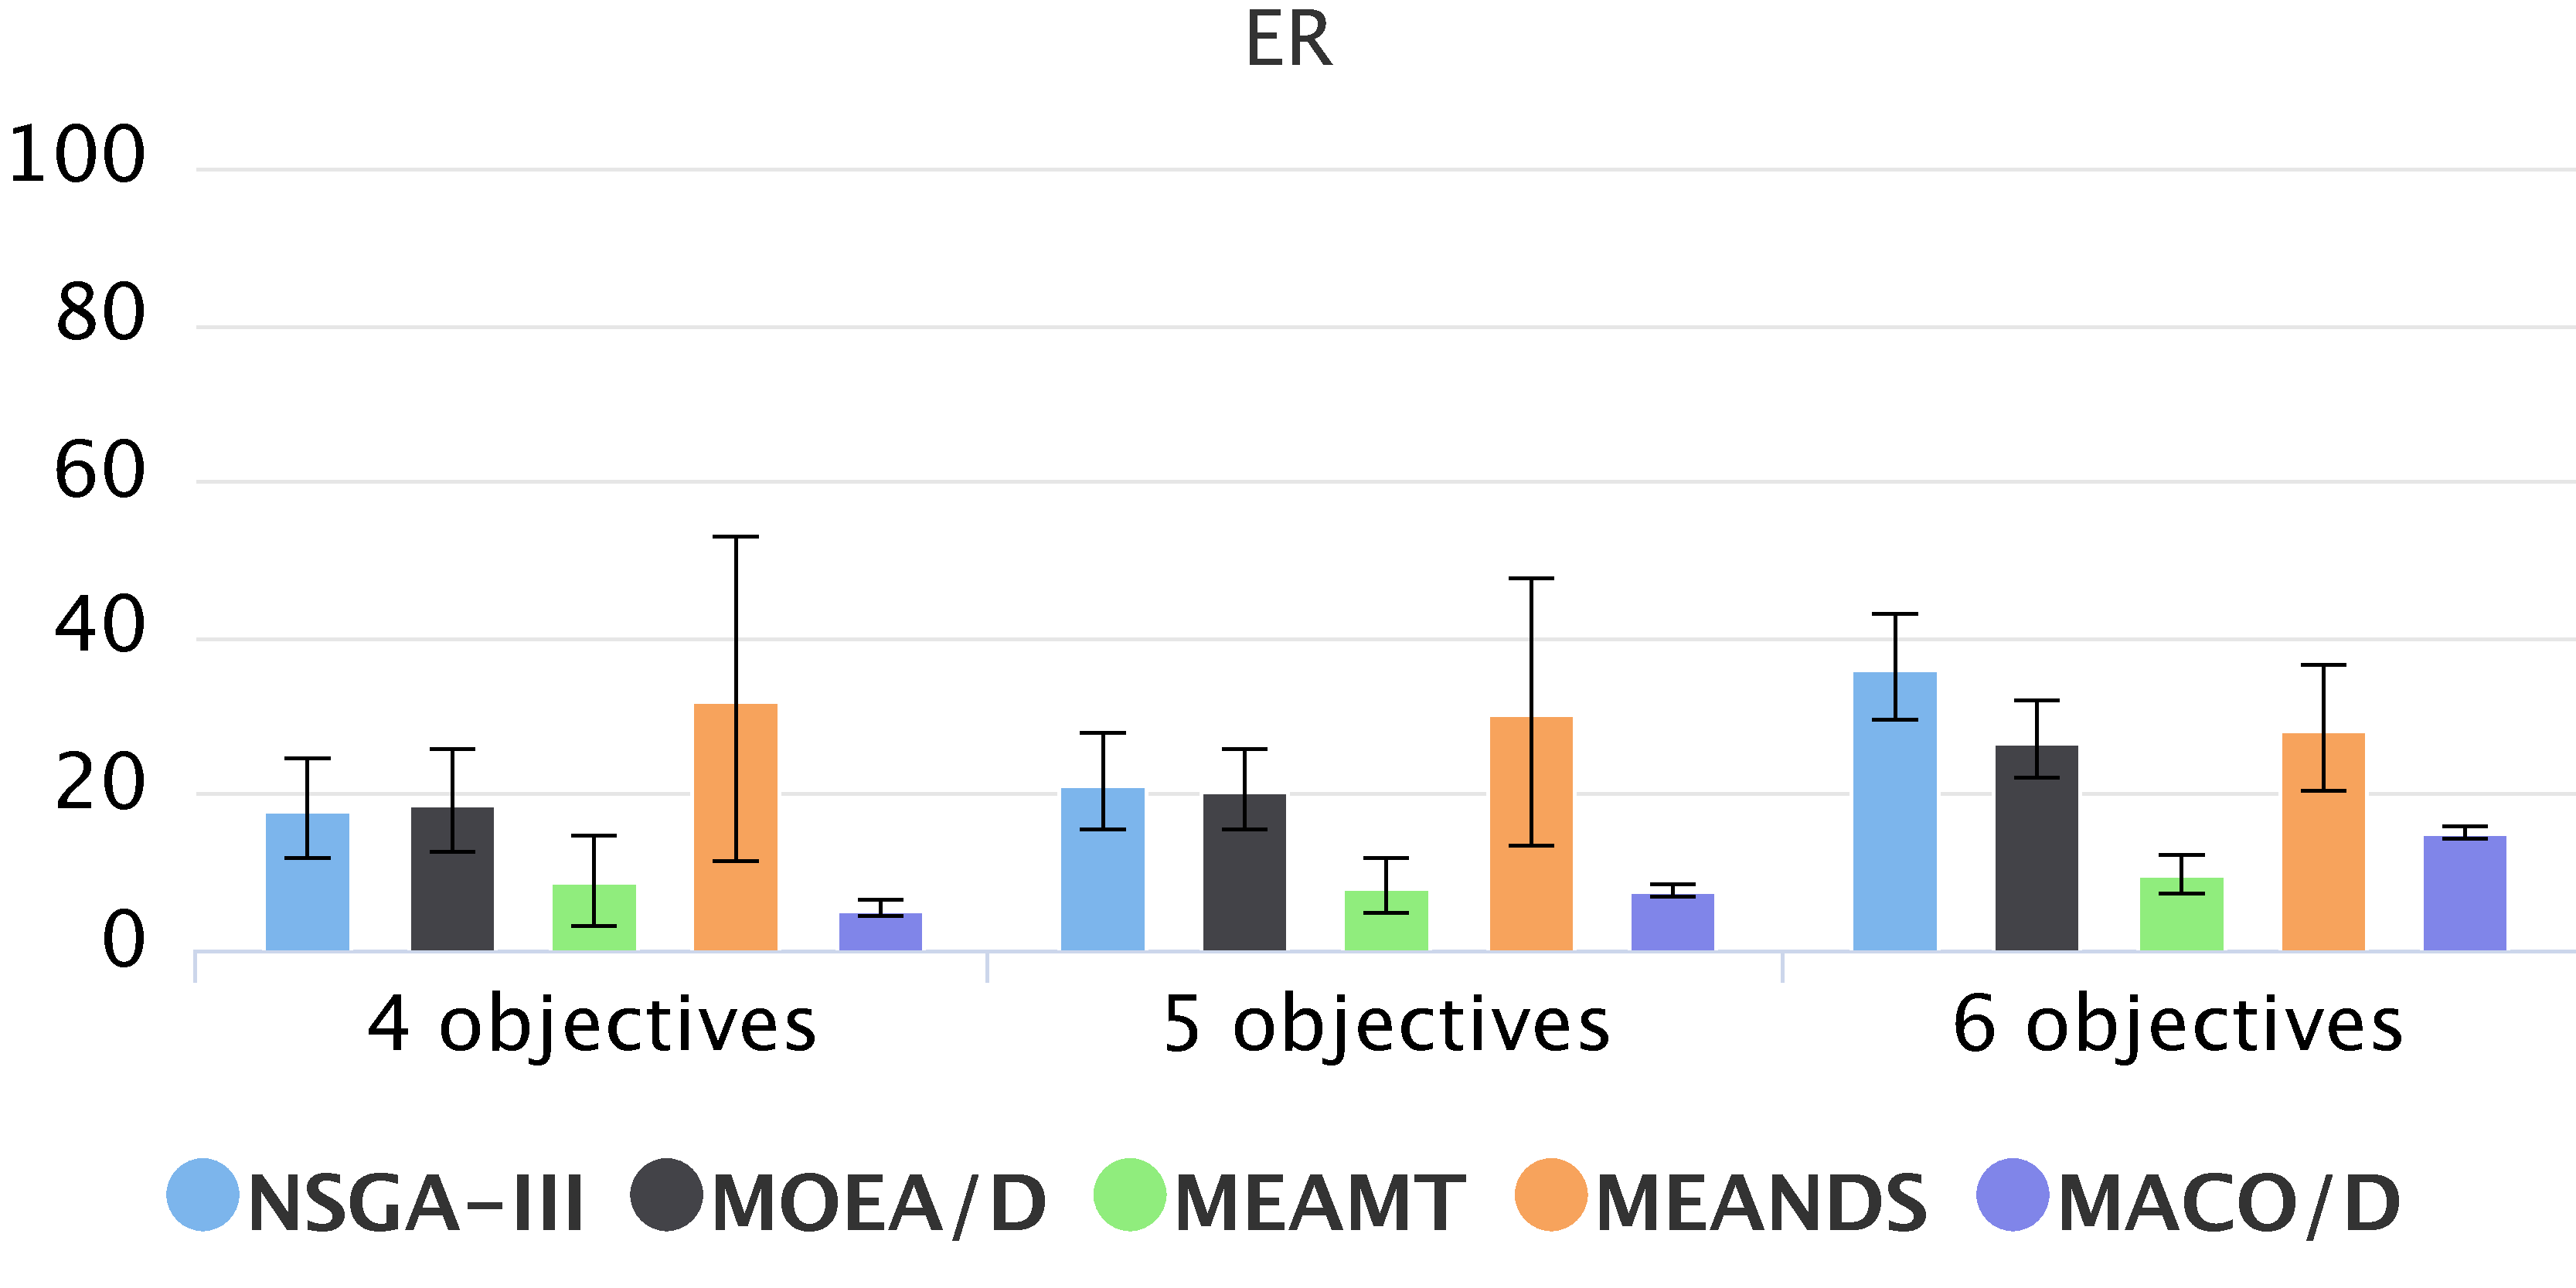
\includegraphics[width=0.5\textwidth]{cap_experimentos/figs/etapa2/er-mkp-todos}
	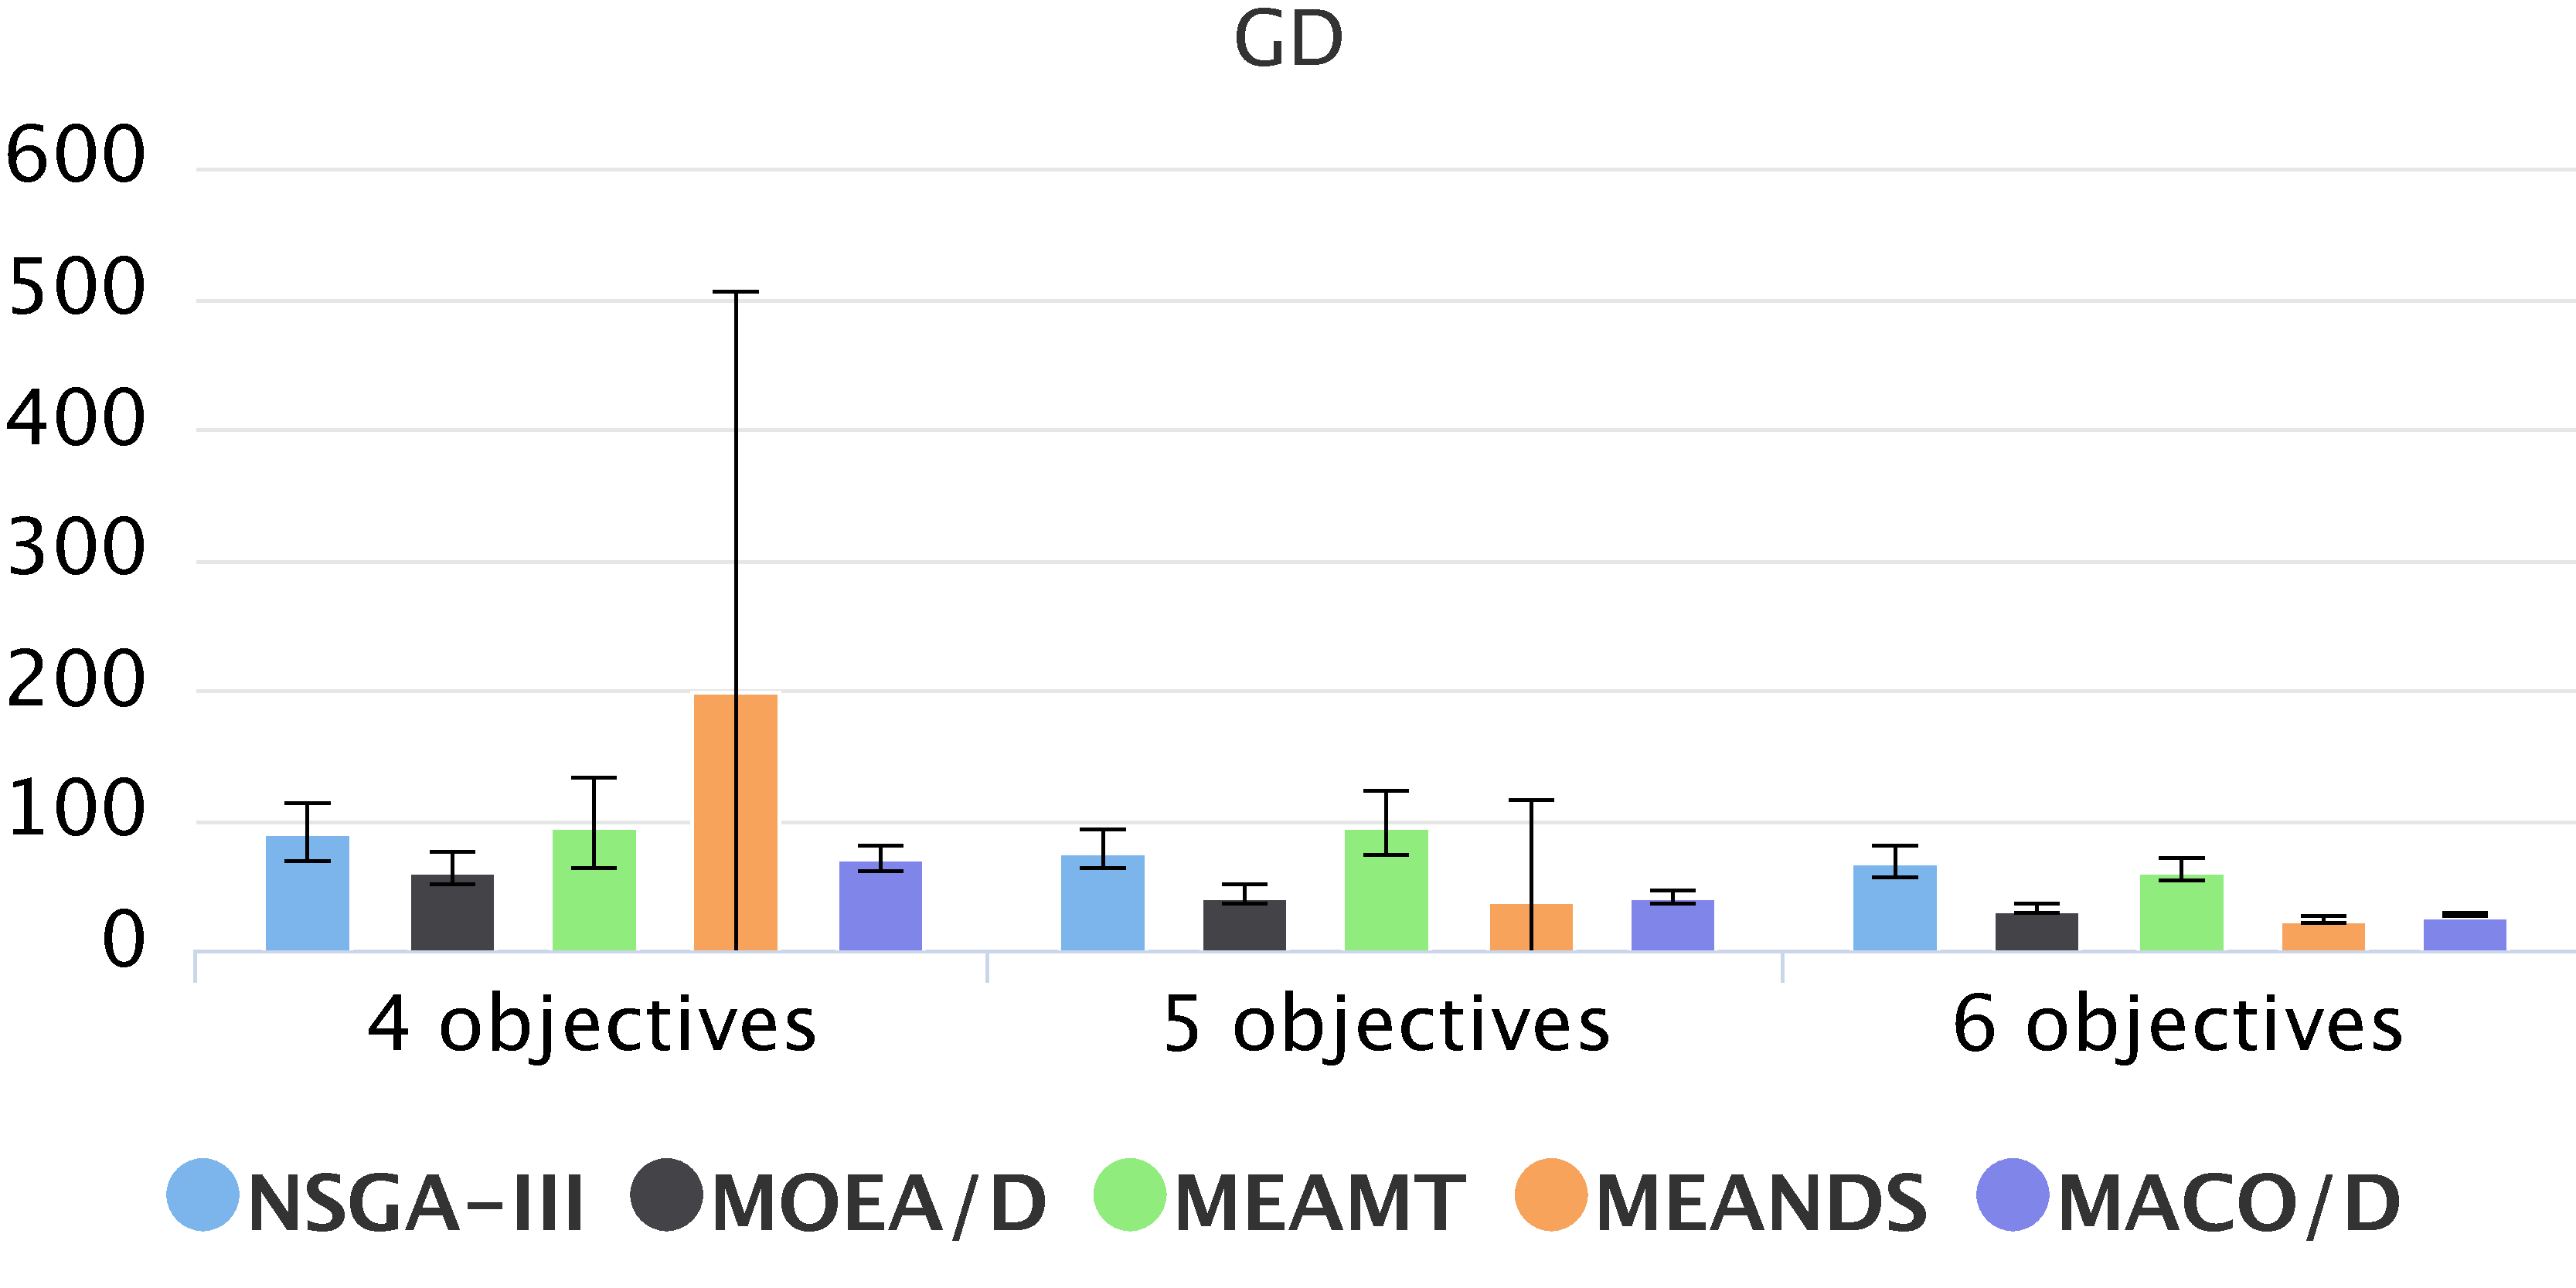
\includegraphics[width=0.5\textwidth]{cap_experimentos/figs/etapa2/gd-mkp-todos}
	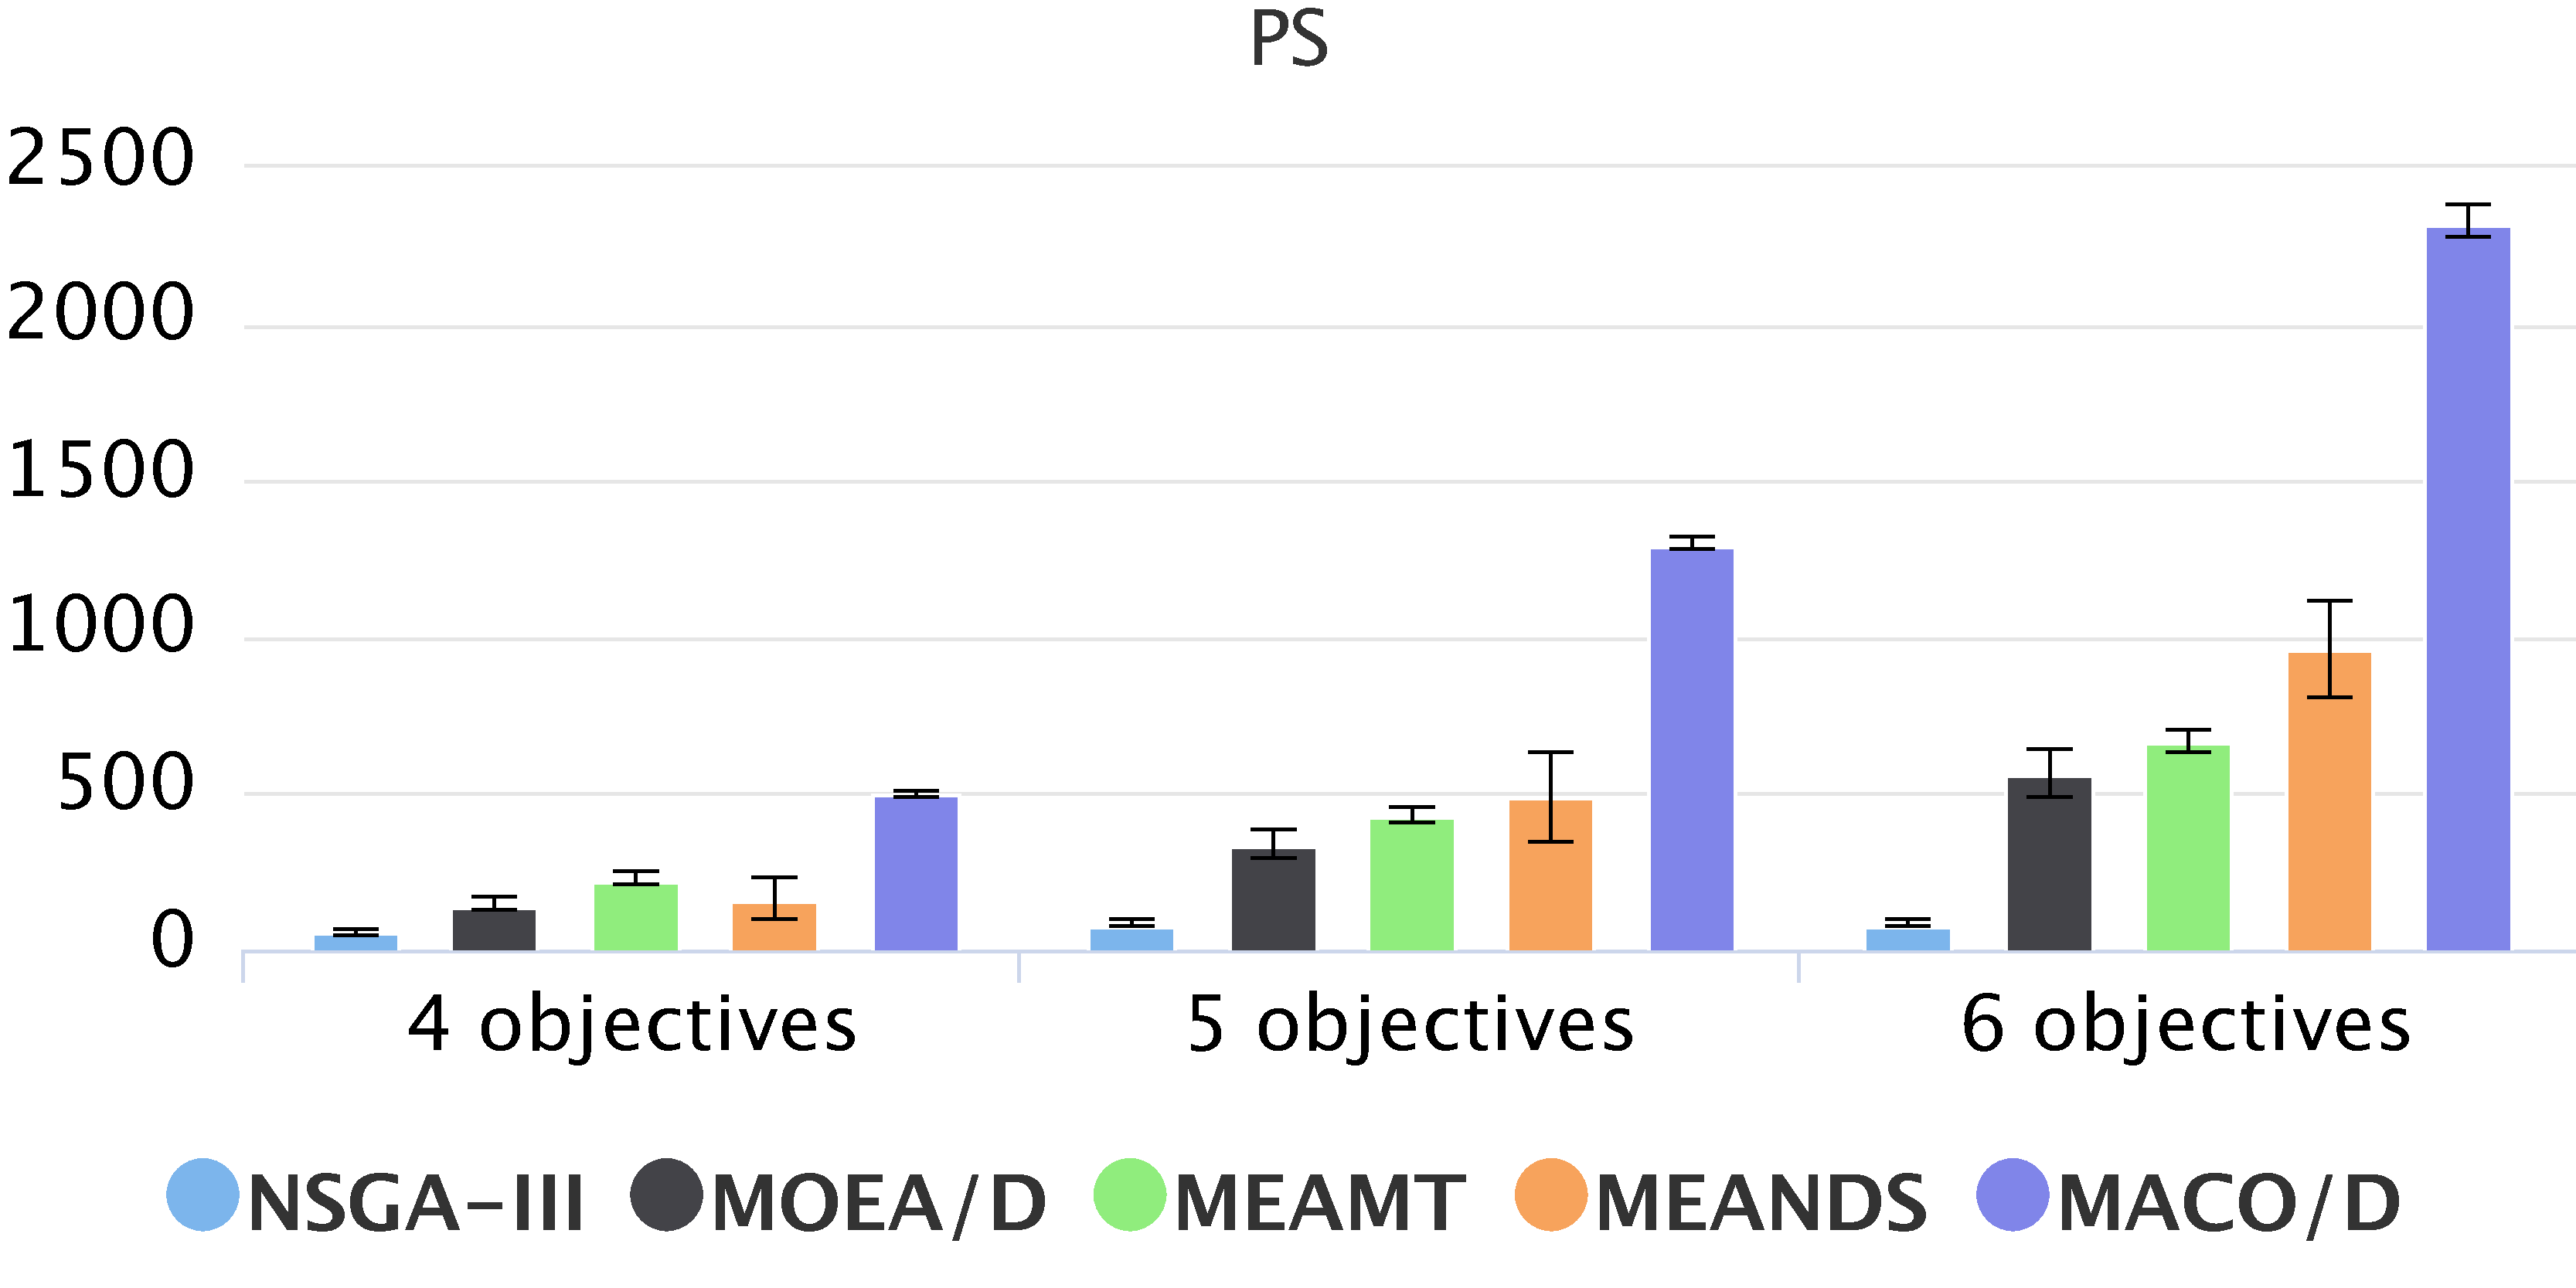
\includegraphics[width=0.5\textwidth]{cap_experimentos/figs/etapa2/ps-mkp-todos}
	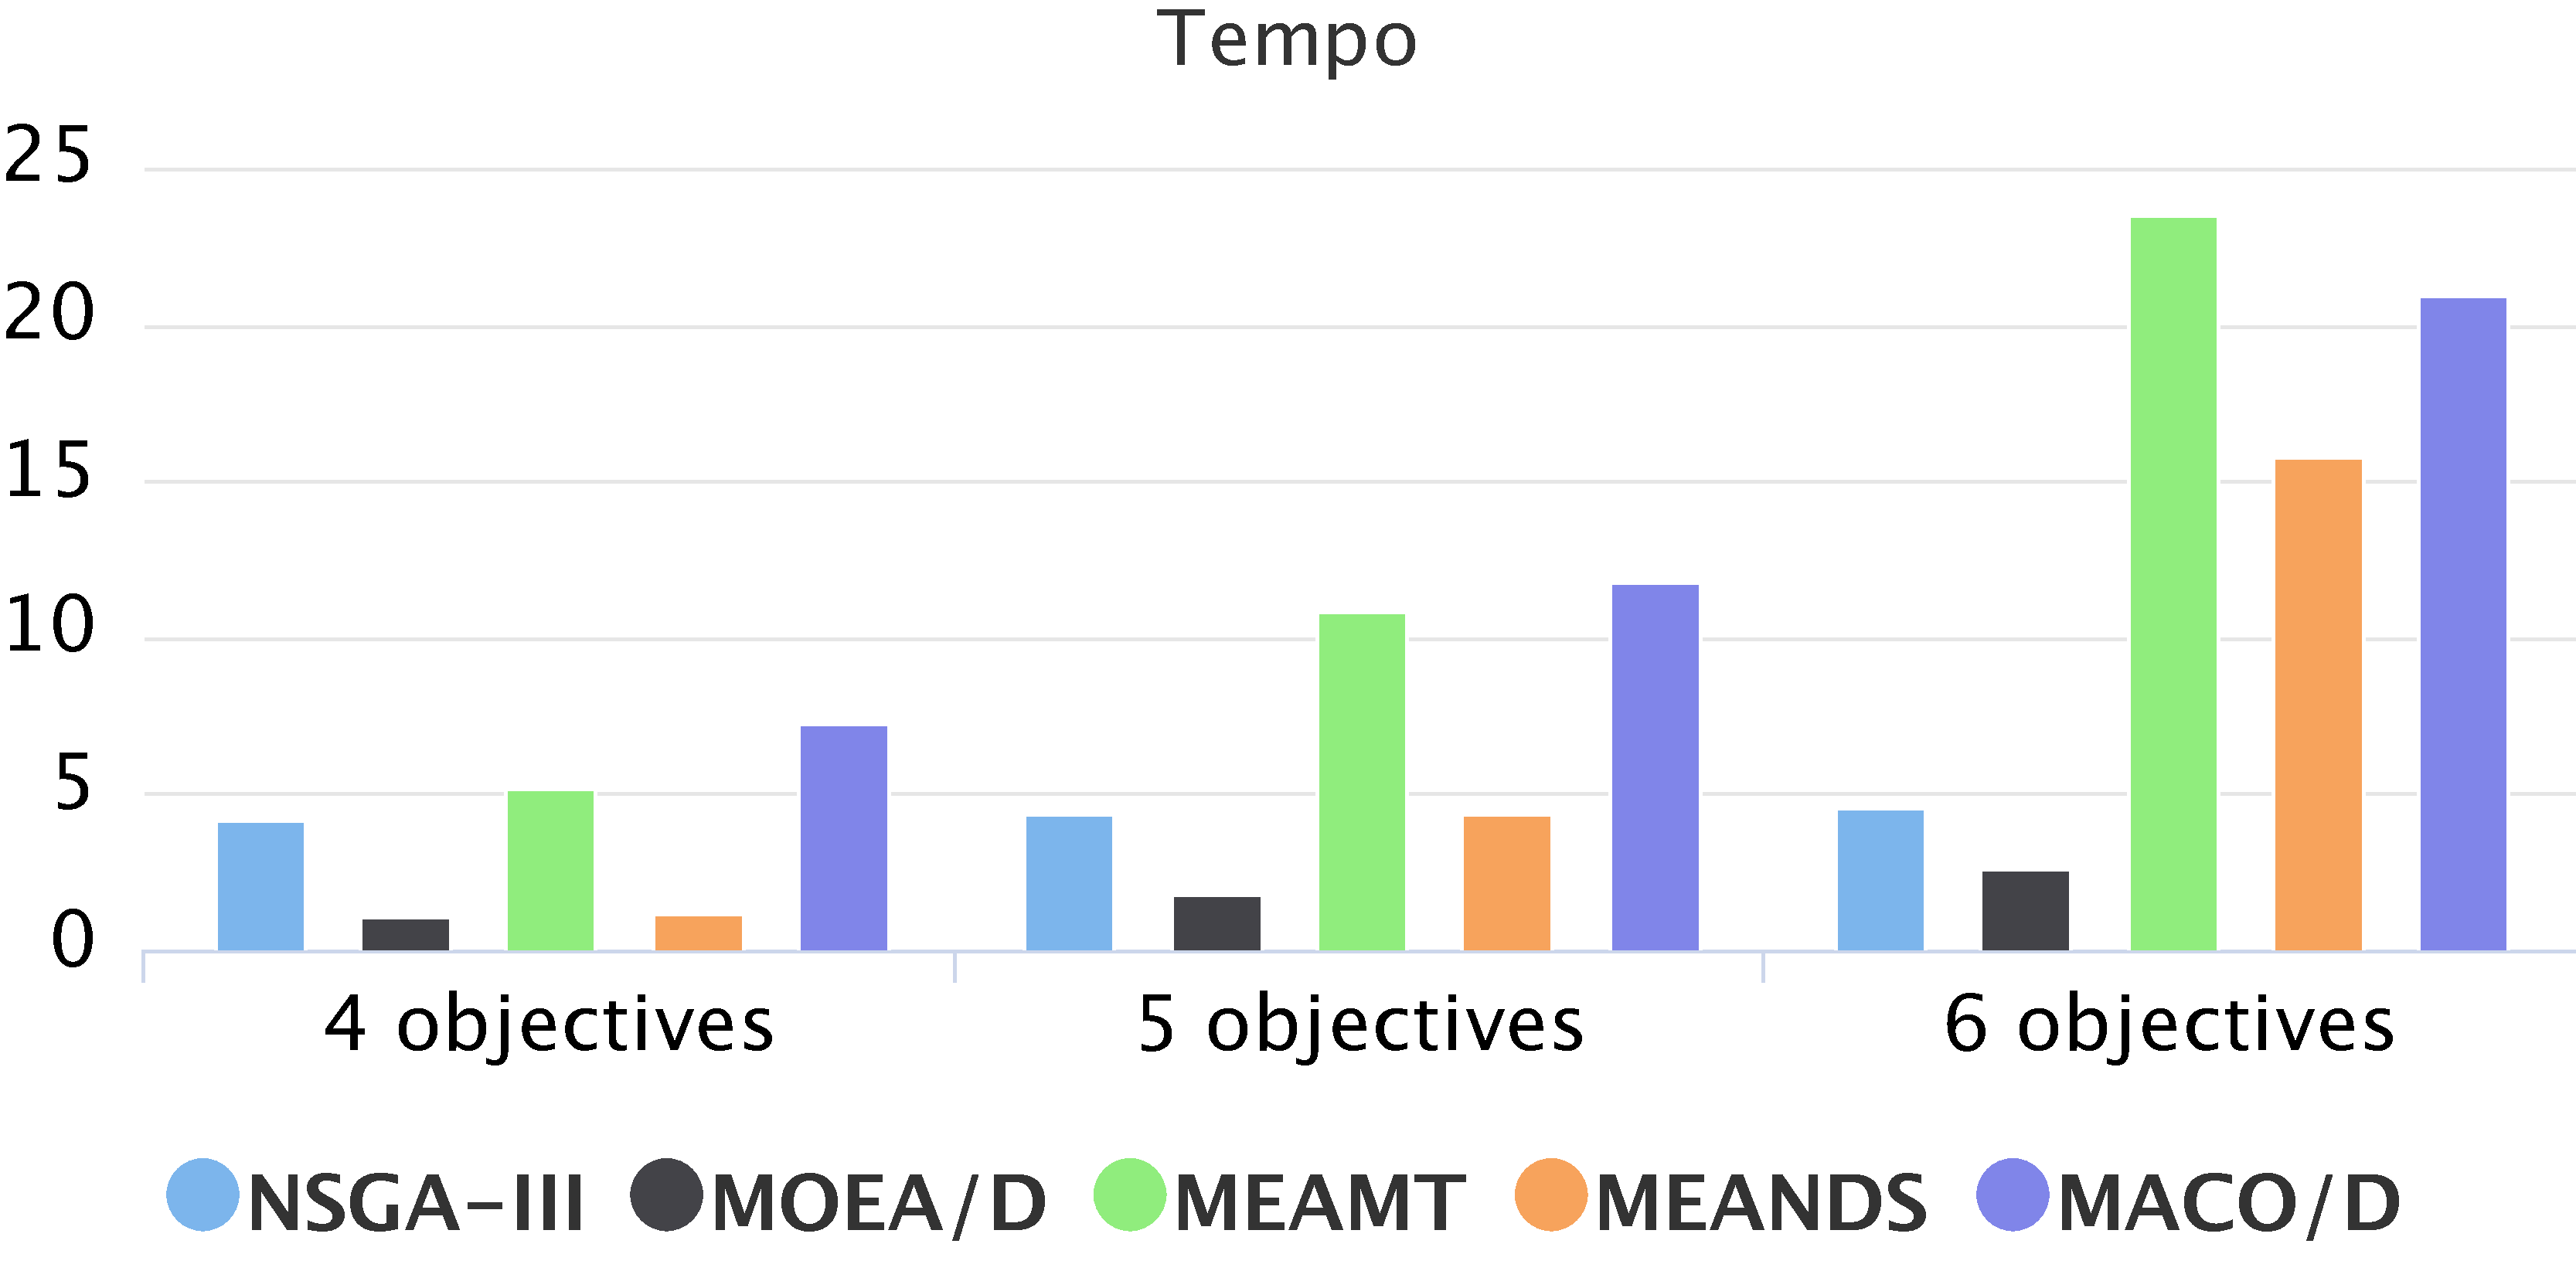
\includegraphics[width=0.5\textwidth]{cap_experimentos/figs/etapa2/time-mkp-todos}
\end{figure*}

A fim de se fazer uma análise conjunta dos resultados, a média entre os 3 cenários é apresentada nos gráficos da figura \ref{fig_exp2_mkp_todos}. As taxas de erro são muito baixas para ambos AEMMT e MACO/D quando comparados aos demais algoritmos. Os resultados em $GD$ são bons para a maioria dos métodos, apenas o AEMMD apresenta um valor ruim de GD no problema de 4 objetivos. O MOEA/D produz o melhor $GD$ no problema de 4 objetivos, enquanto que em 5 e 6 objetivos, o MACO/D e o AEMMD consegue valores bem similares. É importante notar que os desvio padrões no AEMMD são altos, o que pode representar uma certa inconsistência do método em gerar boas soluções. O $PS$ é , de longe, dominado pelo MACO/D. Em questão de tempo de execução, o AEMMT, o AEMMD e o MACO/S variam bastante com o número de objetivos, enquanto os demais são estáveis. O MOEA/D é o algoritmo mais rápido entre os avaliados nesta etapa dos experimentos. O NSGA-III não é pior método em nenhuma das formulações de objetivo, mas também não se destaca em nenhum dos critérios de avaliação.

\begin{figure*}[!htbp]
	\caption{Etapa 2: resultados para o PRM na rede $R_1$}
	\label{fig_exp2_mrp_r1}
	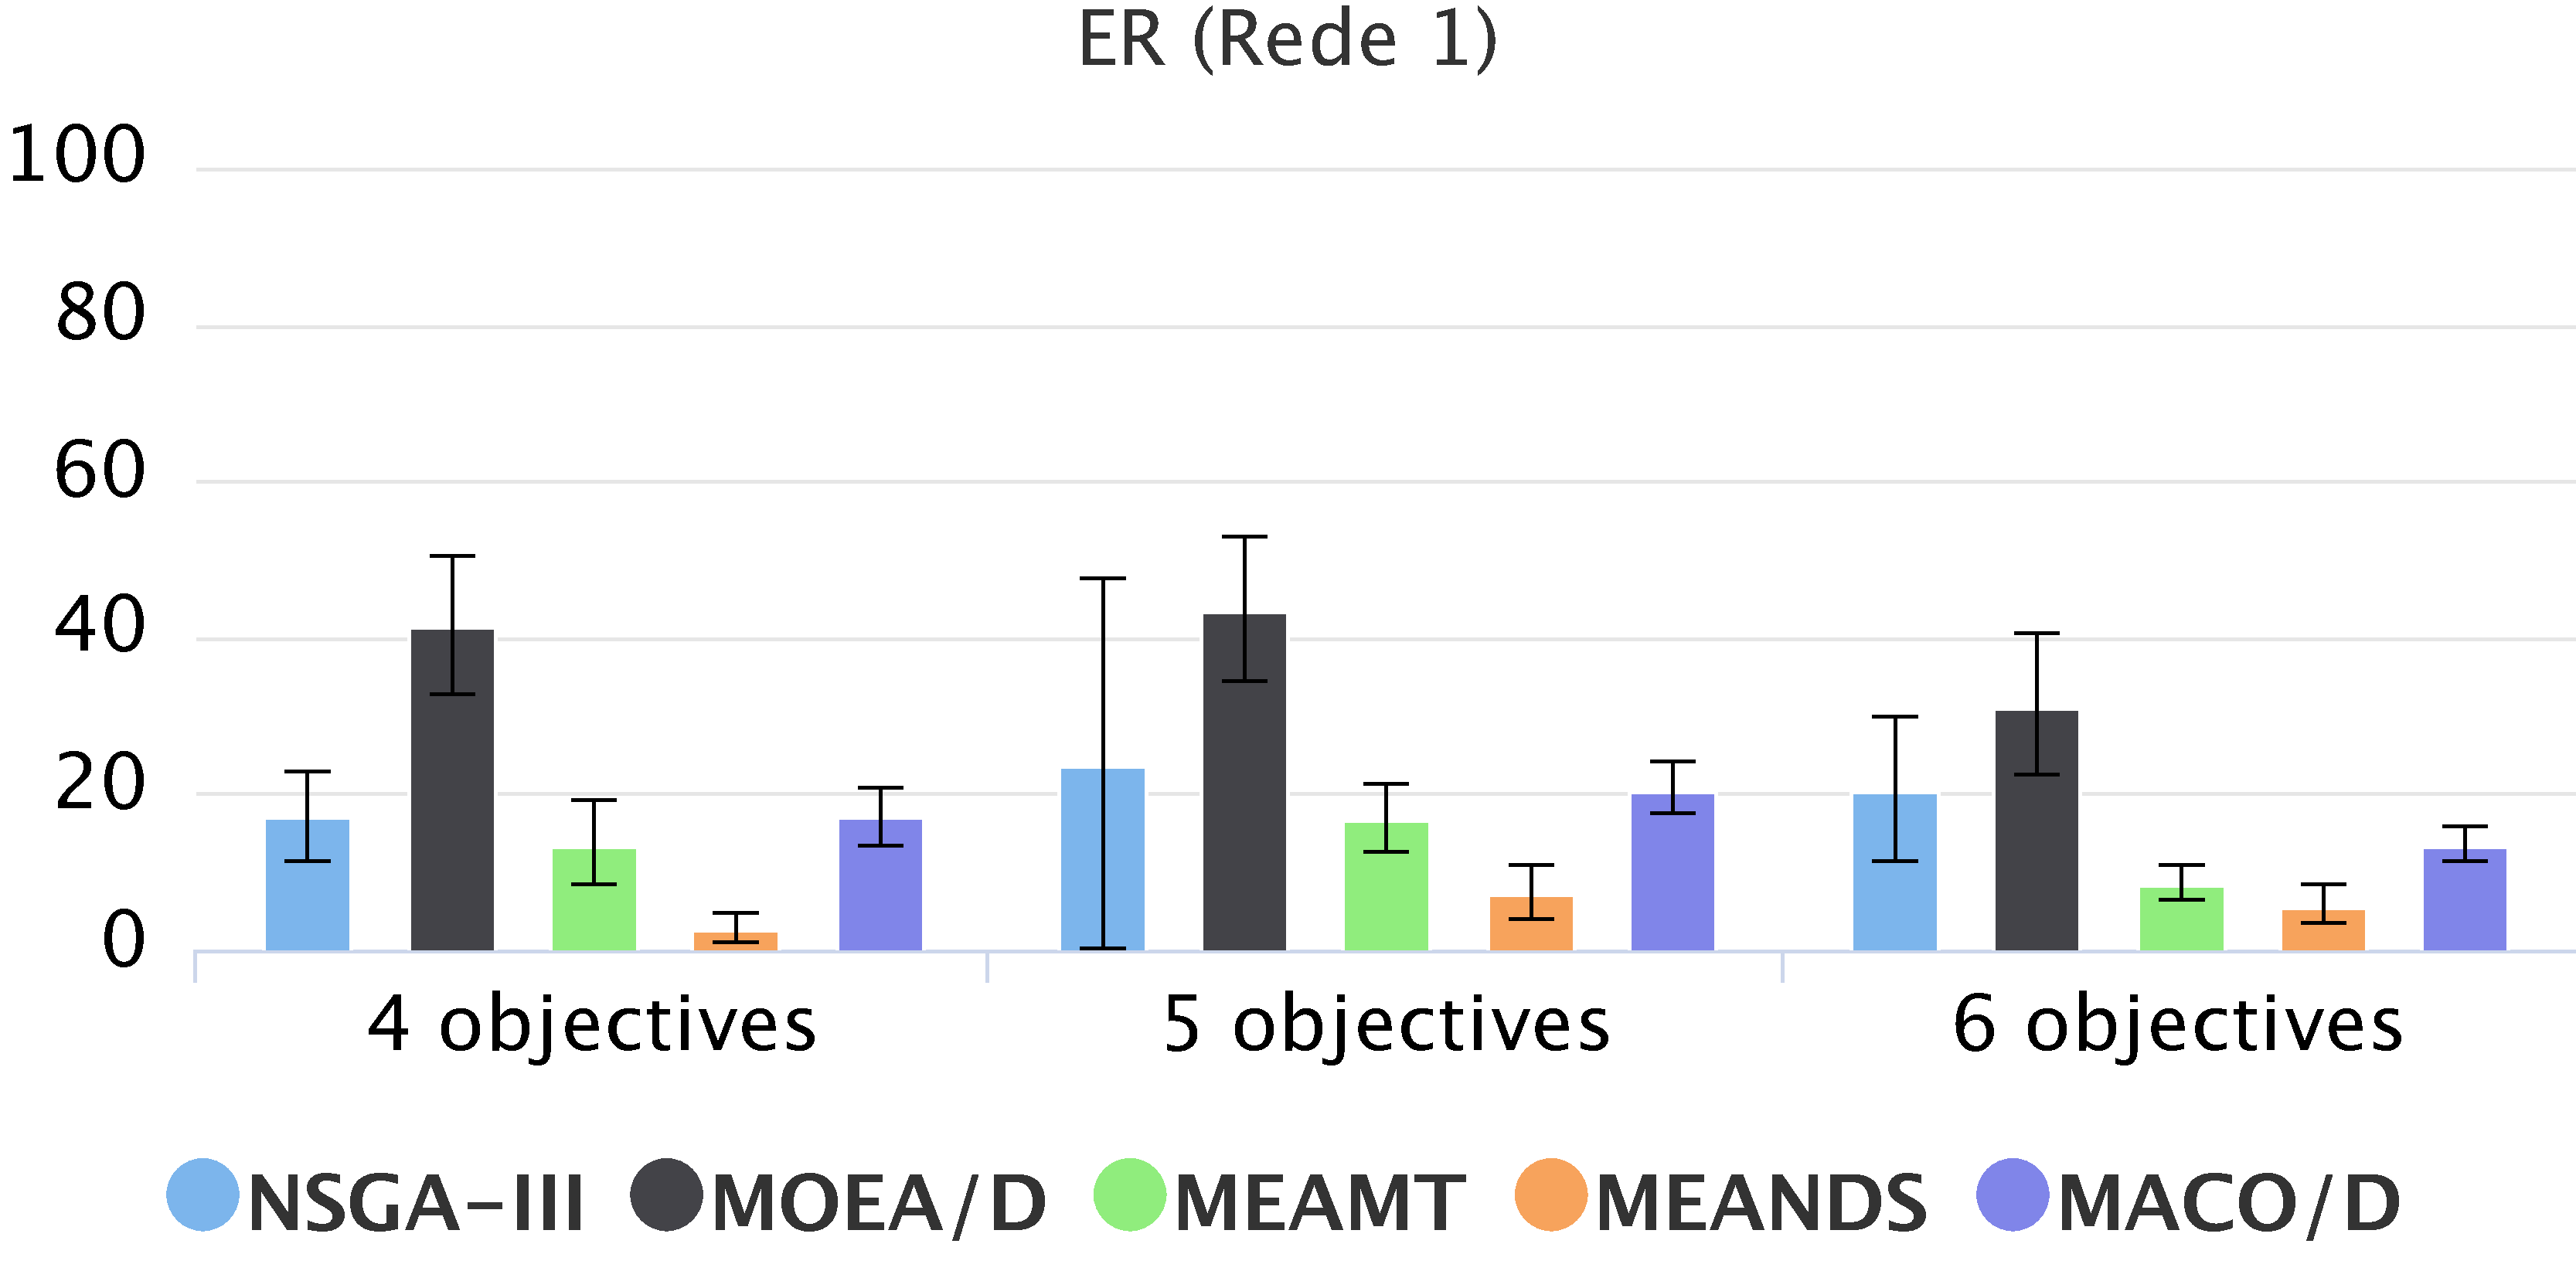
\includegraphics[width=0.5\textwidth]{cap_experimentos/figs/etapa2/er-mrp-r1}
	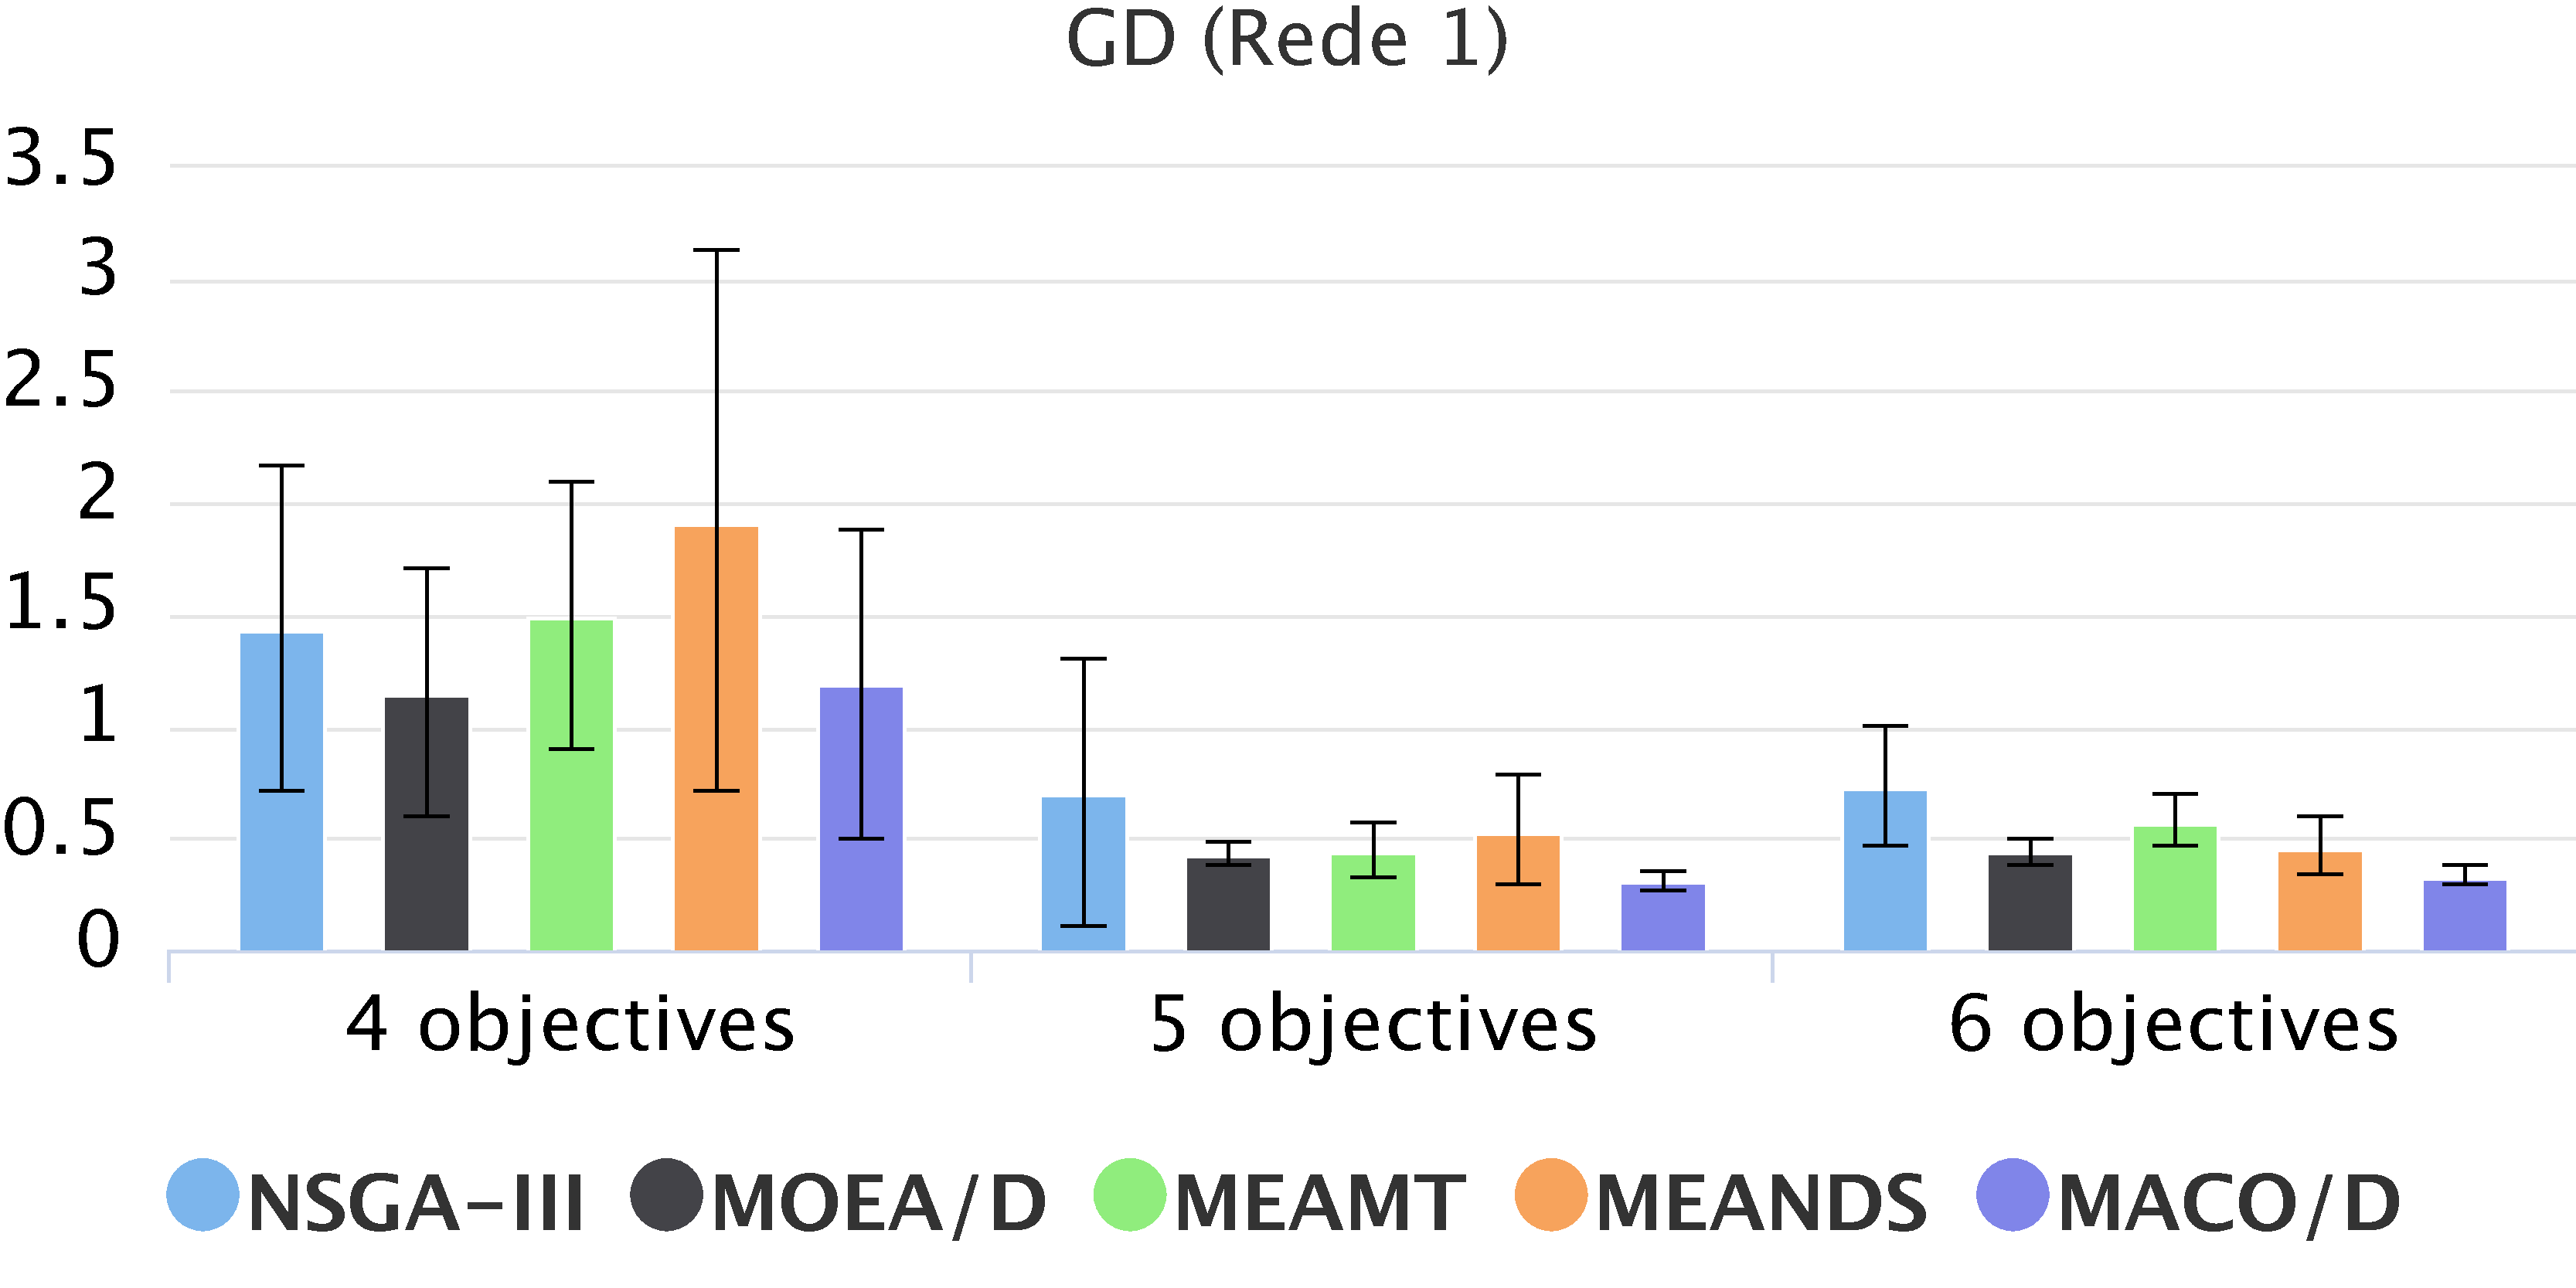
\includegraphics[width=0.5\textwidth]{cap_experimentos/figs/etapa2/gd-mrp-r1}
	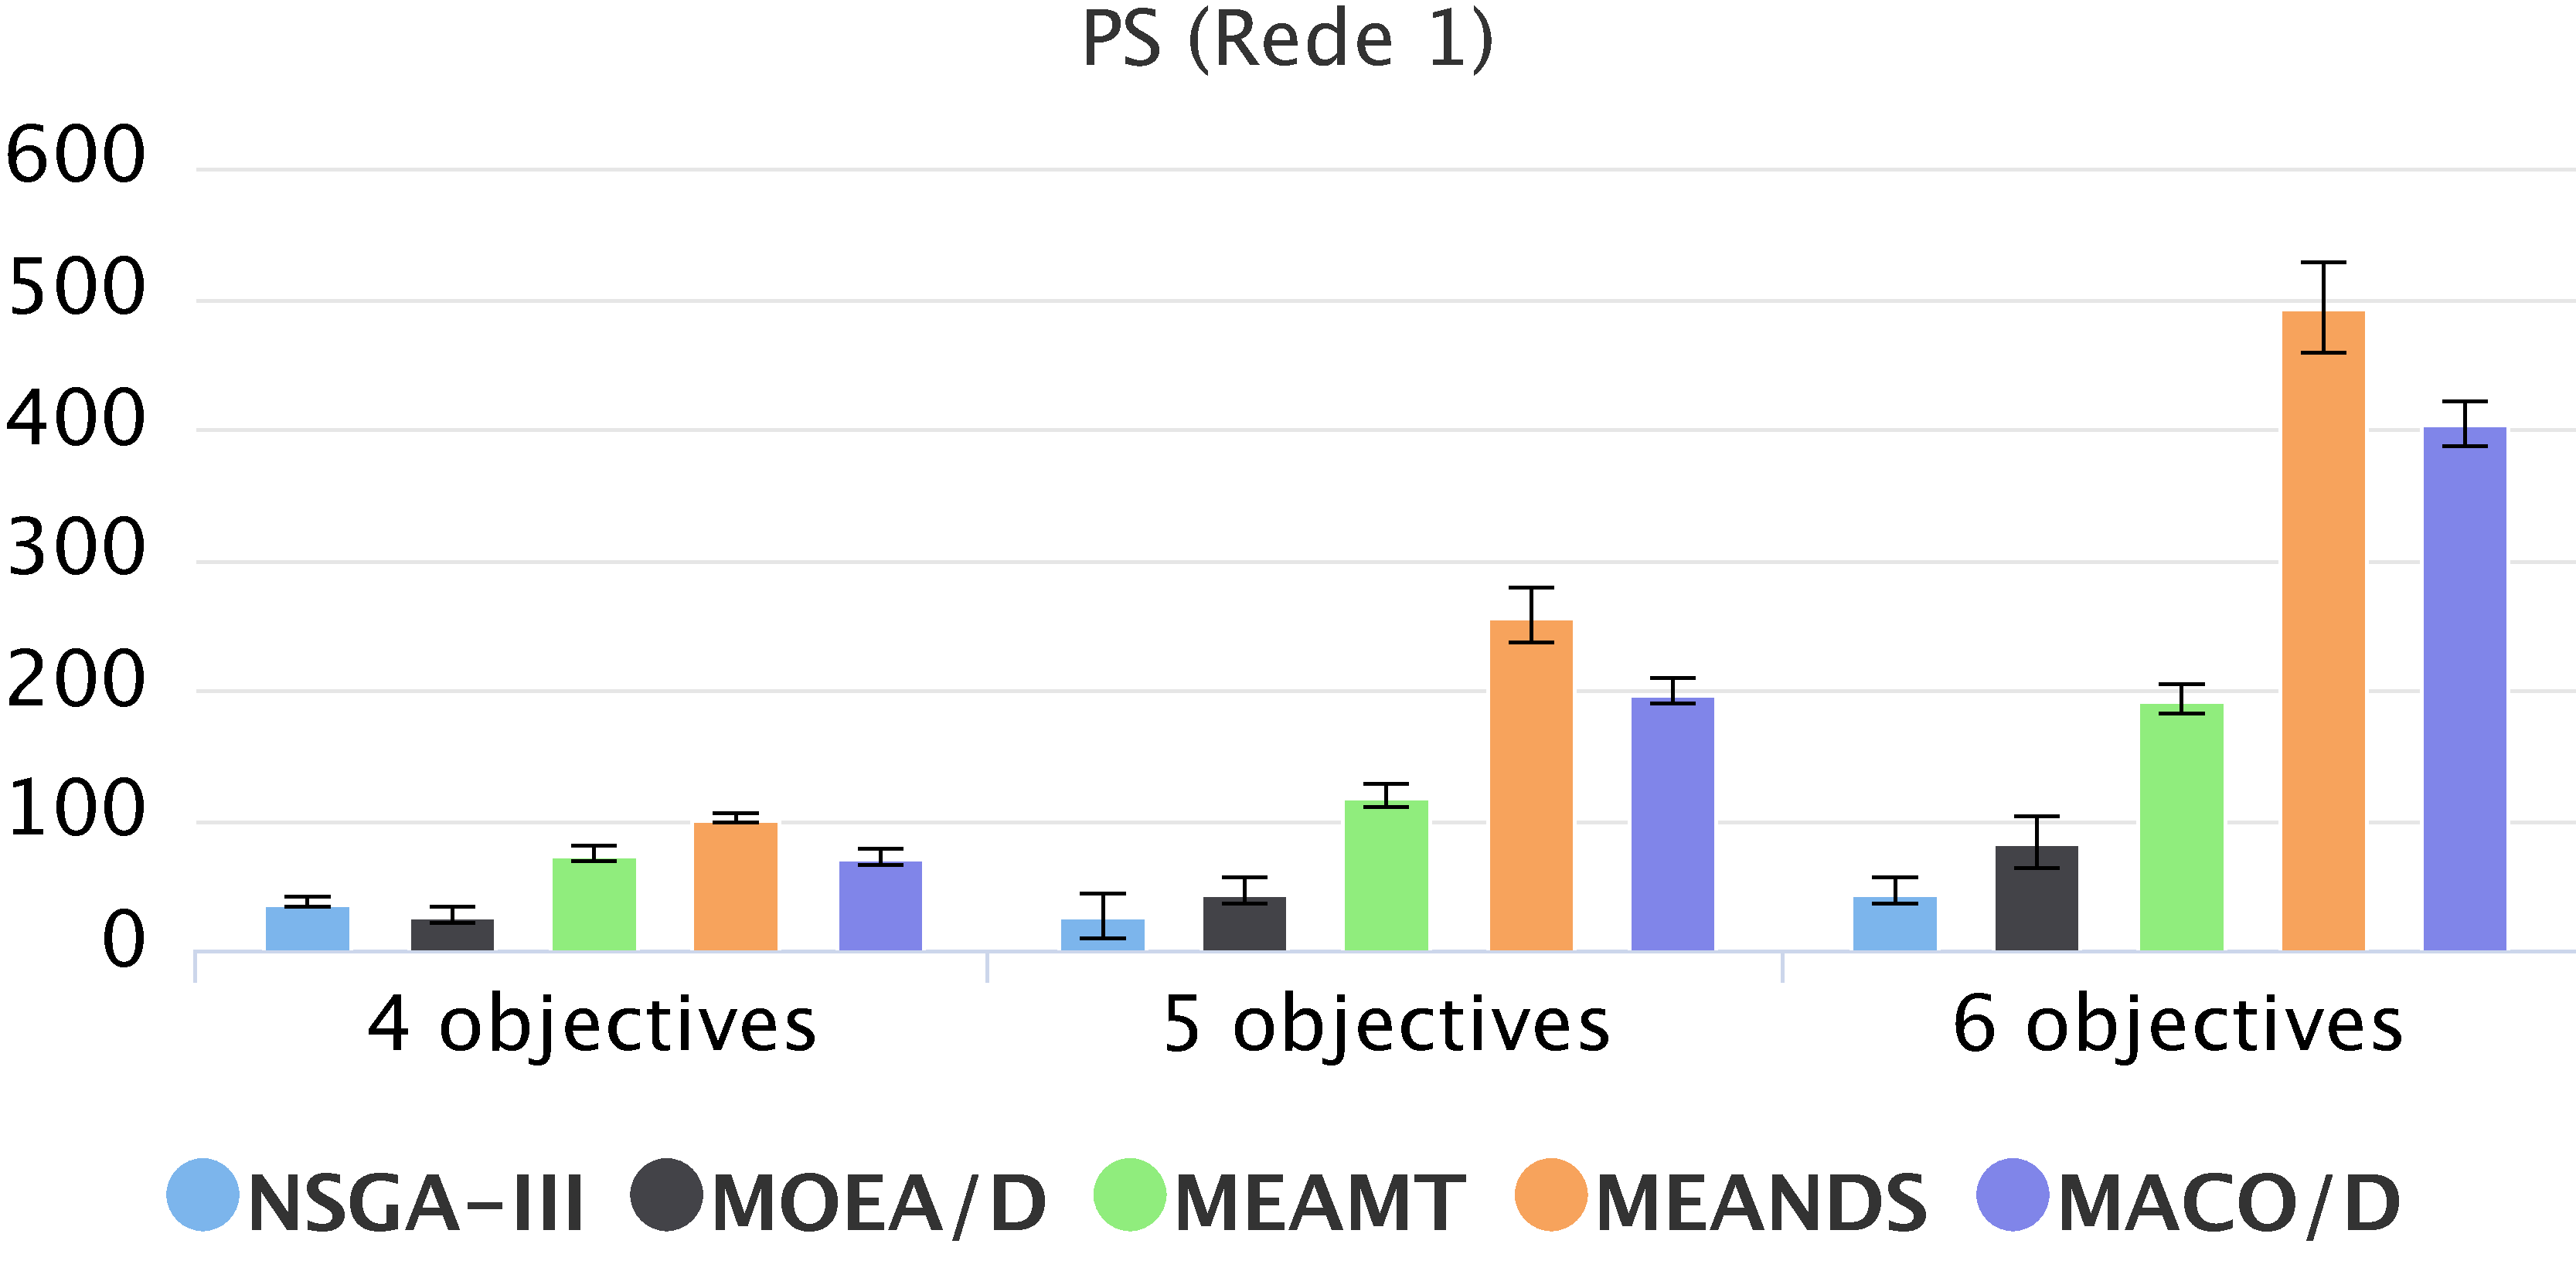
\includegraphics[width=0.5\textwidth]{cap_experimentos/figs/etapa2/ps-mrp-r1}
	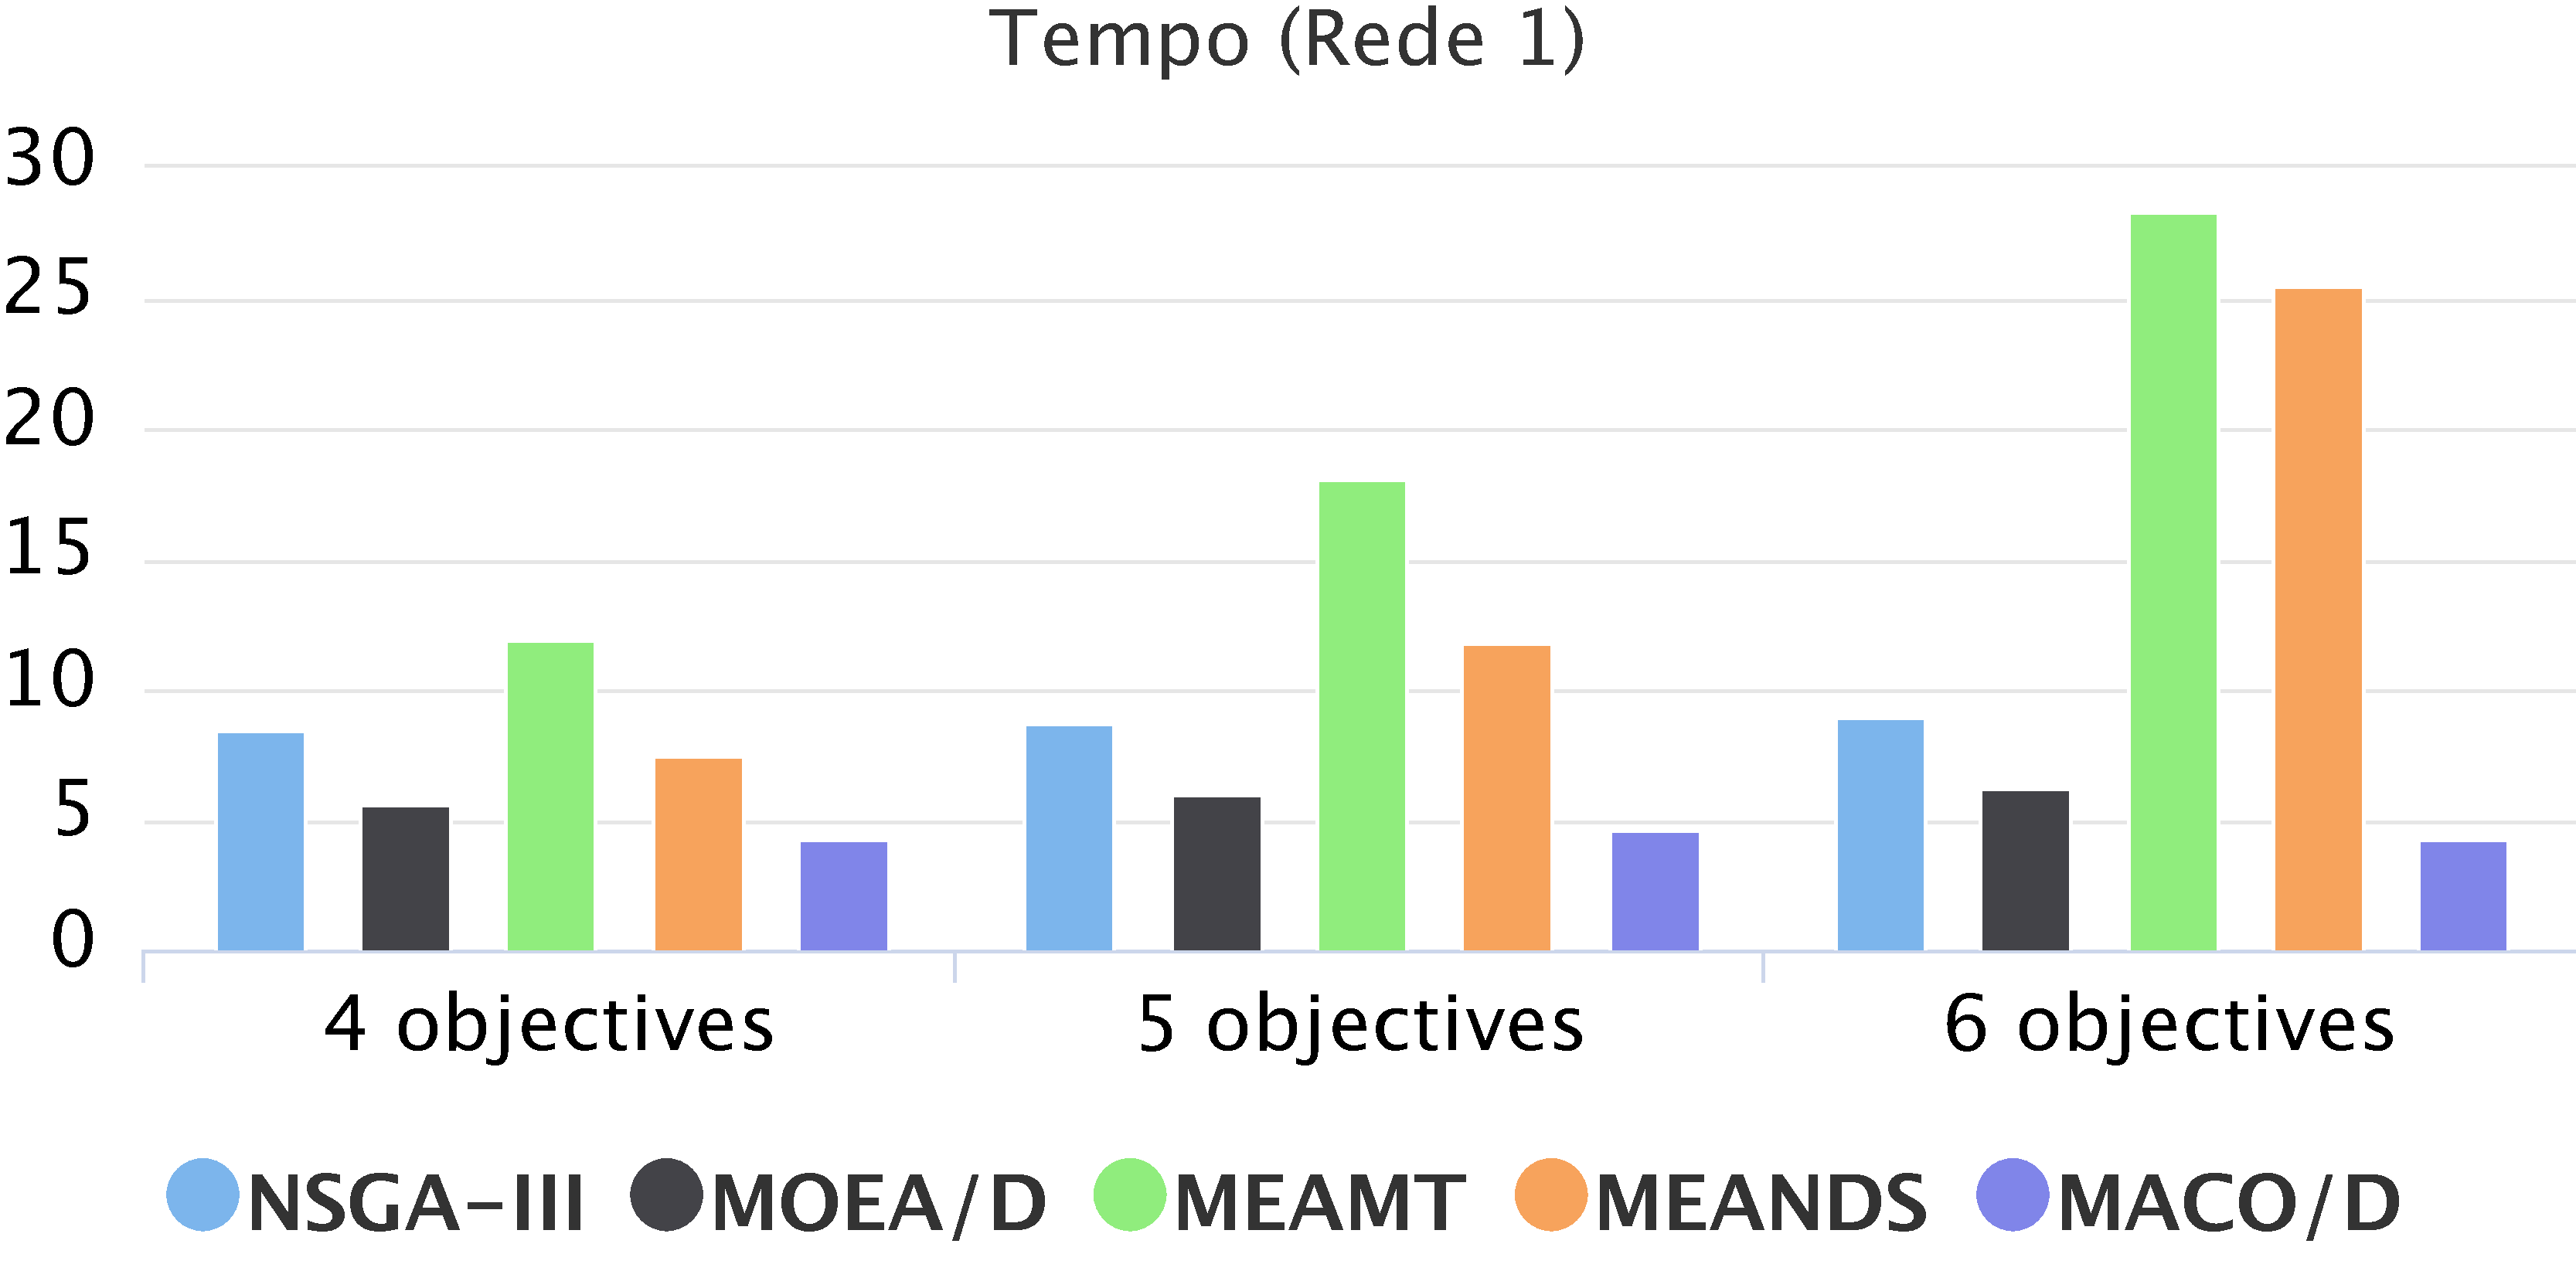
\includegraphics[width=0.5\textwidth]{cap_experimentos/figs/etapa2/time-mrp-r1}
\end{figure*}

Análise do PRM-R1

\begin{figure*}[!htbp]
	\caption{Etapa 2: resultados para o PRM na rede $R_2$}
	\label{fig_exp2_mrp_r2}
	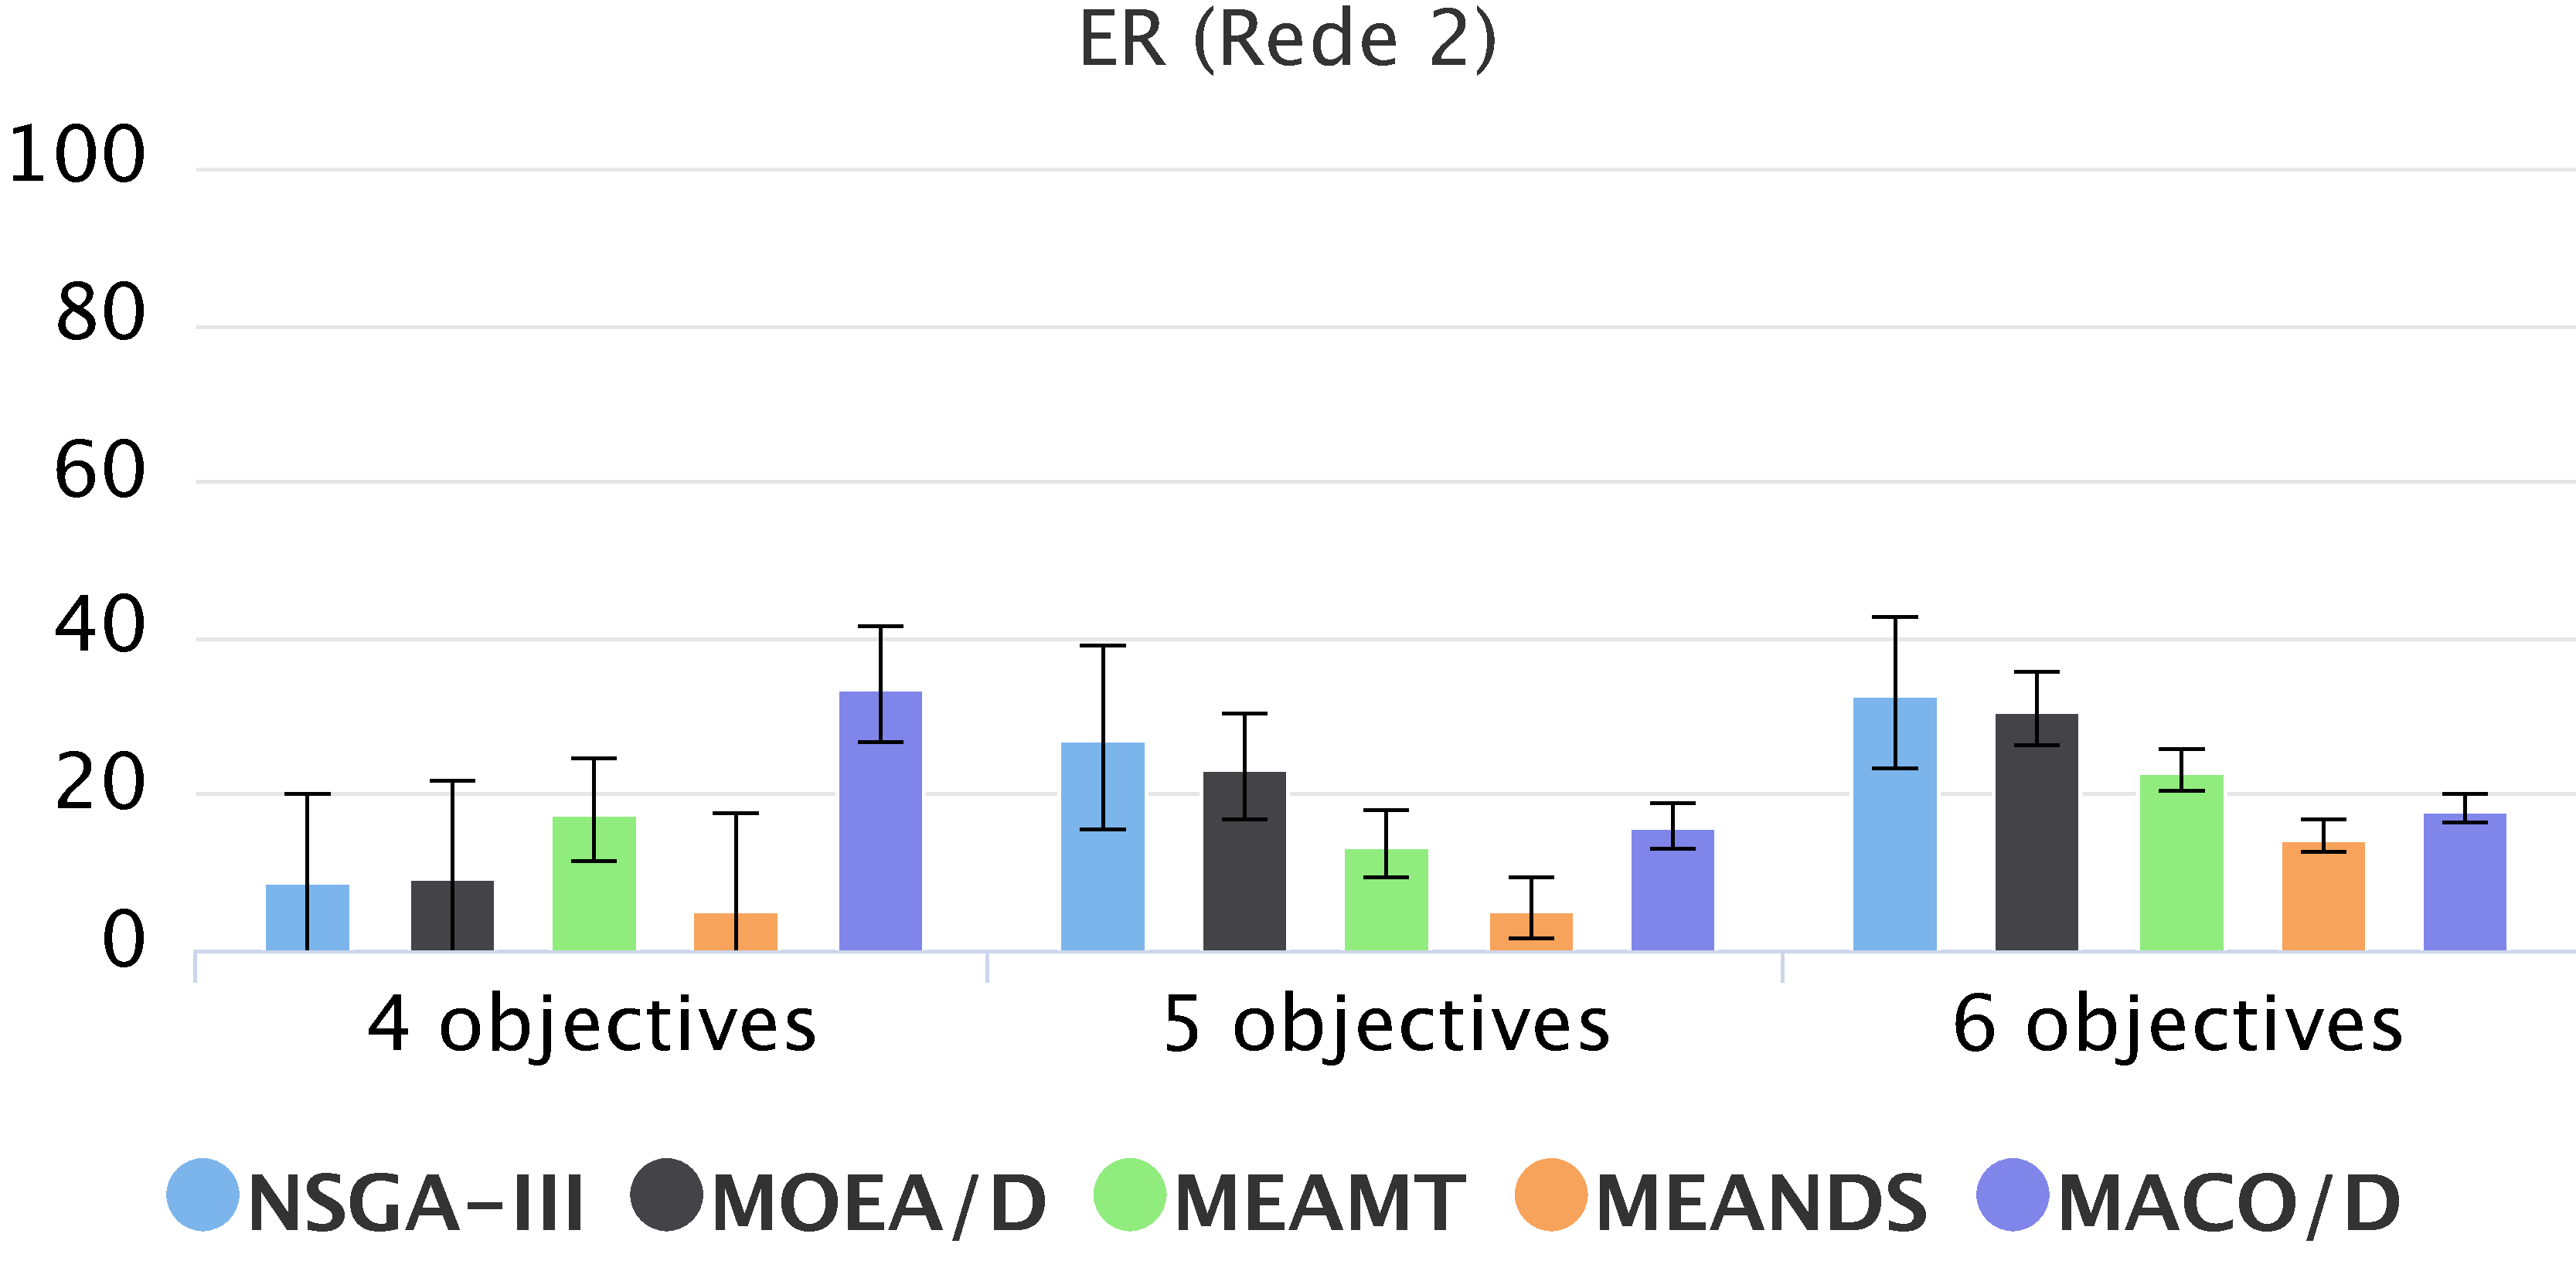
\includegraphics[width=0.5\textwidth]{cap_experimentos/figs/etapa2/er-mrp-r2}
	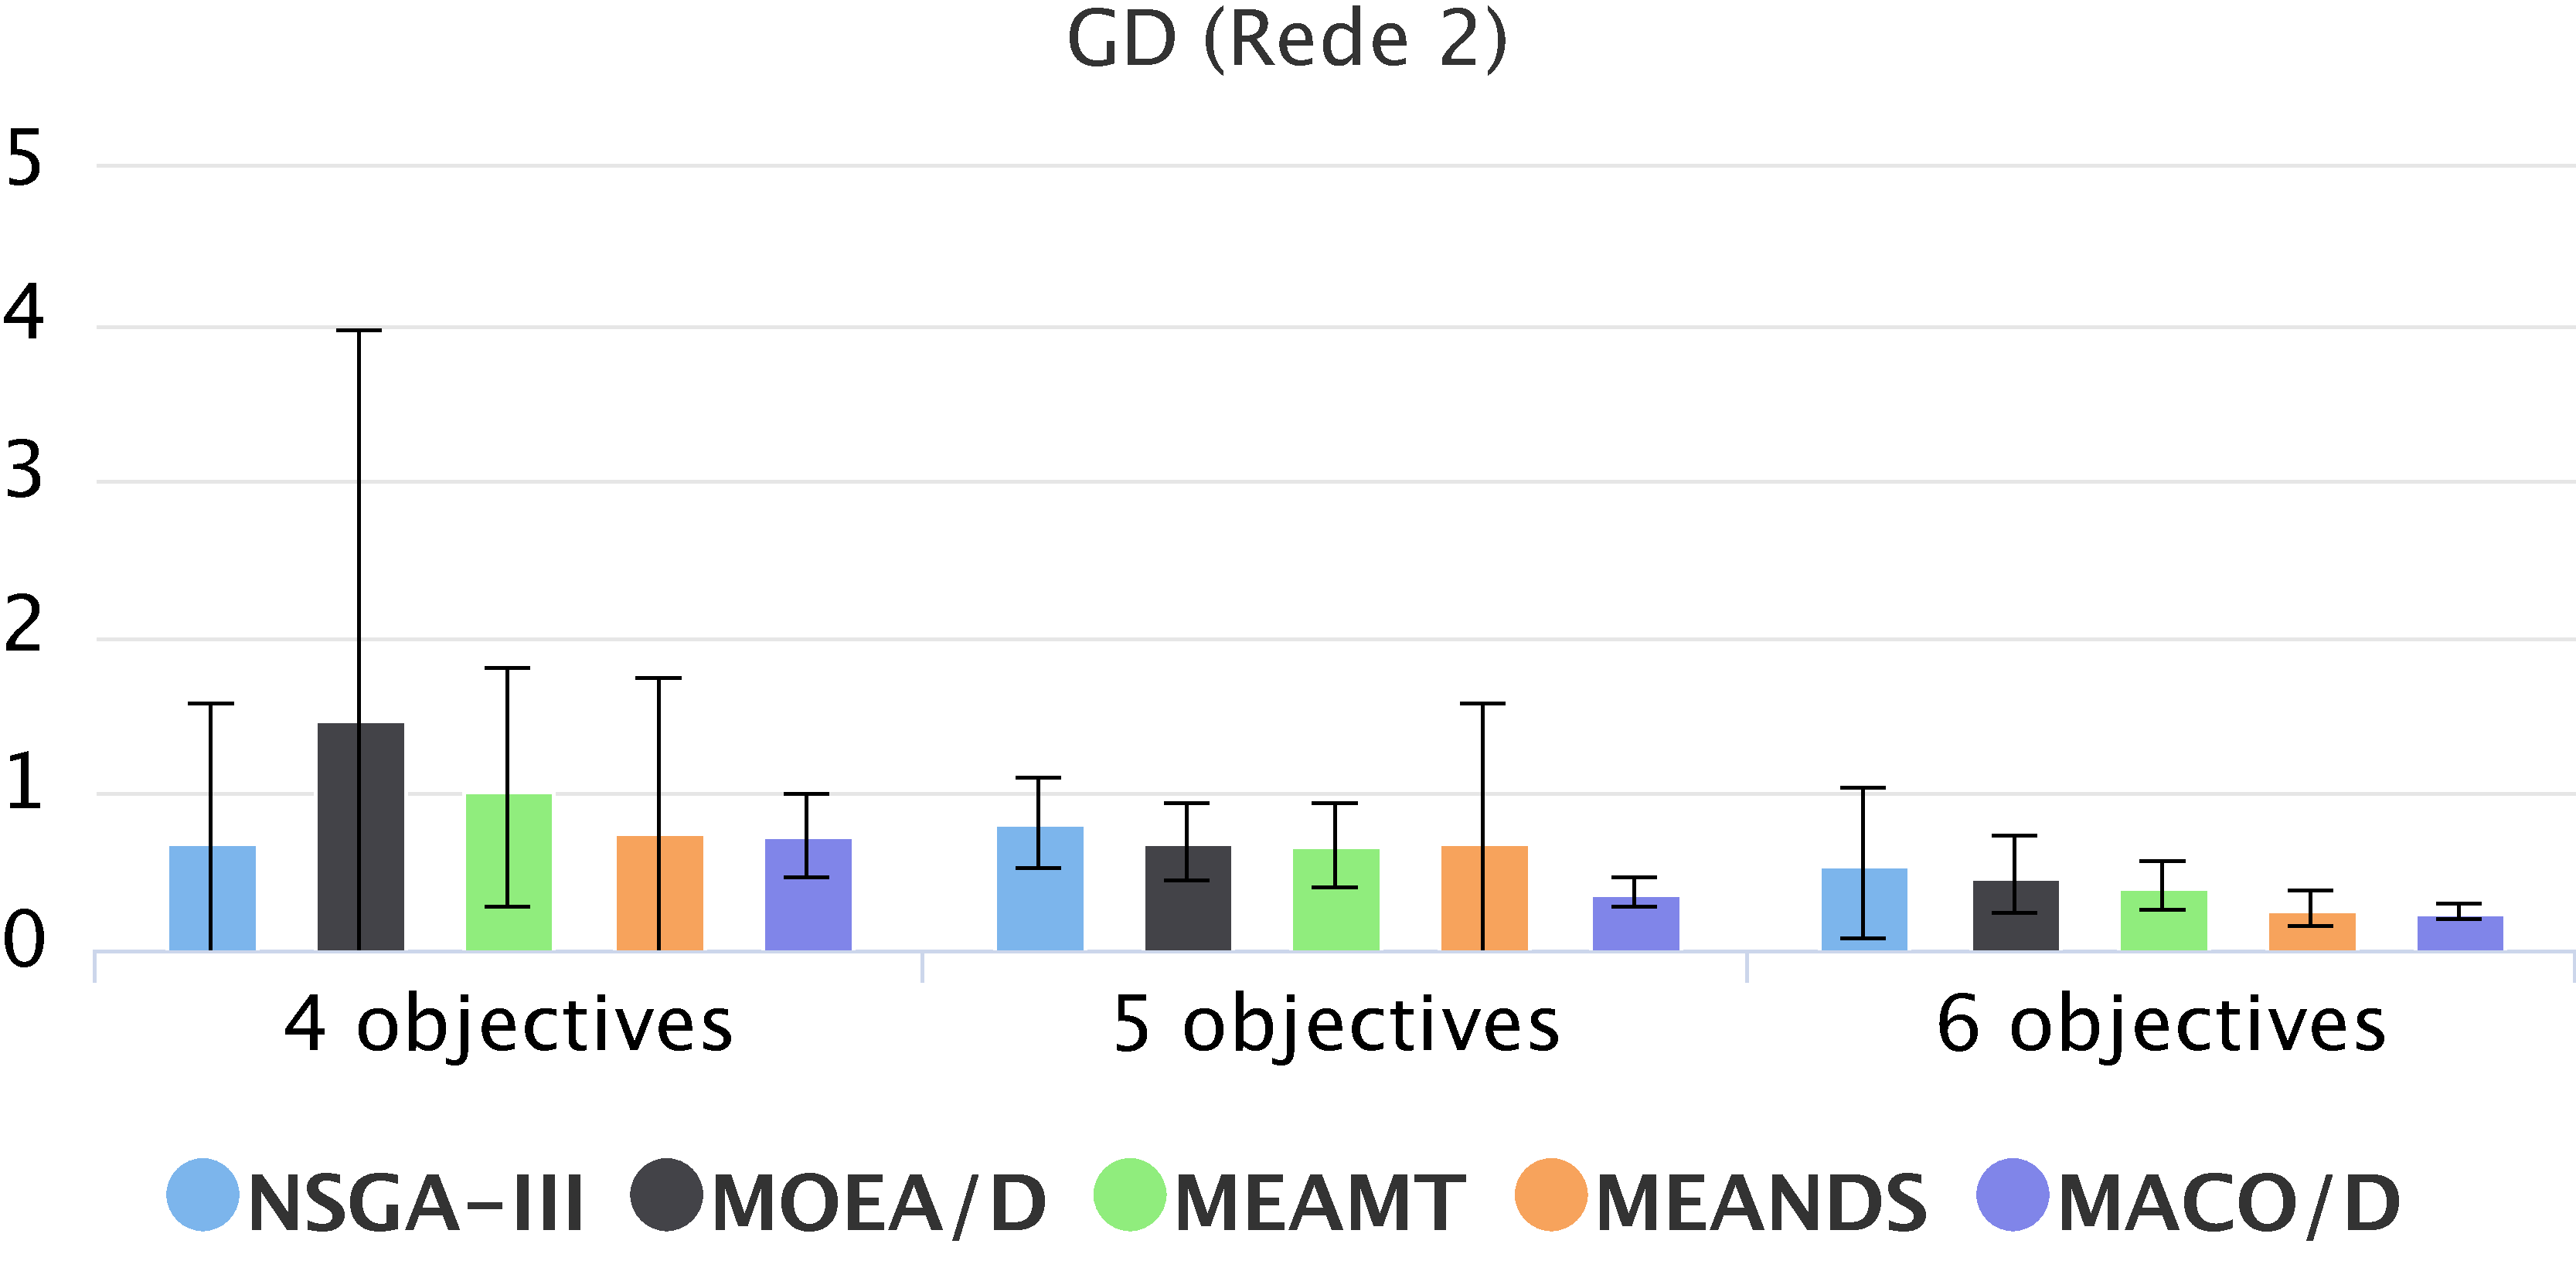
\includegraphics[width=0.5\textwidth]{cap_experimentos/figs/etapa2/gd-mrp-r2}
	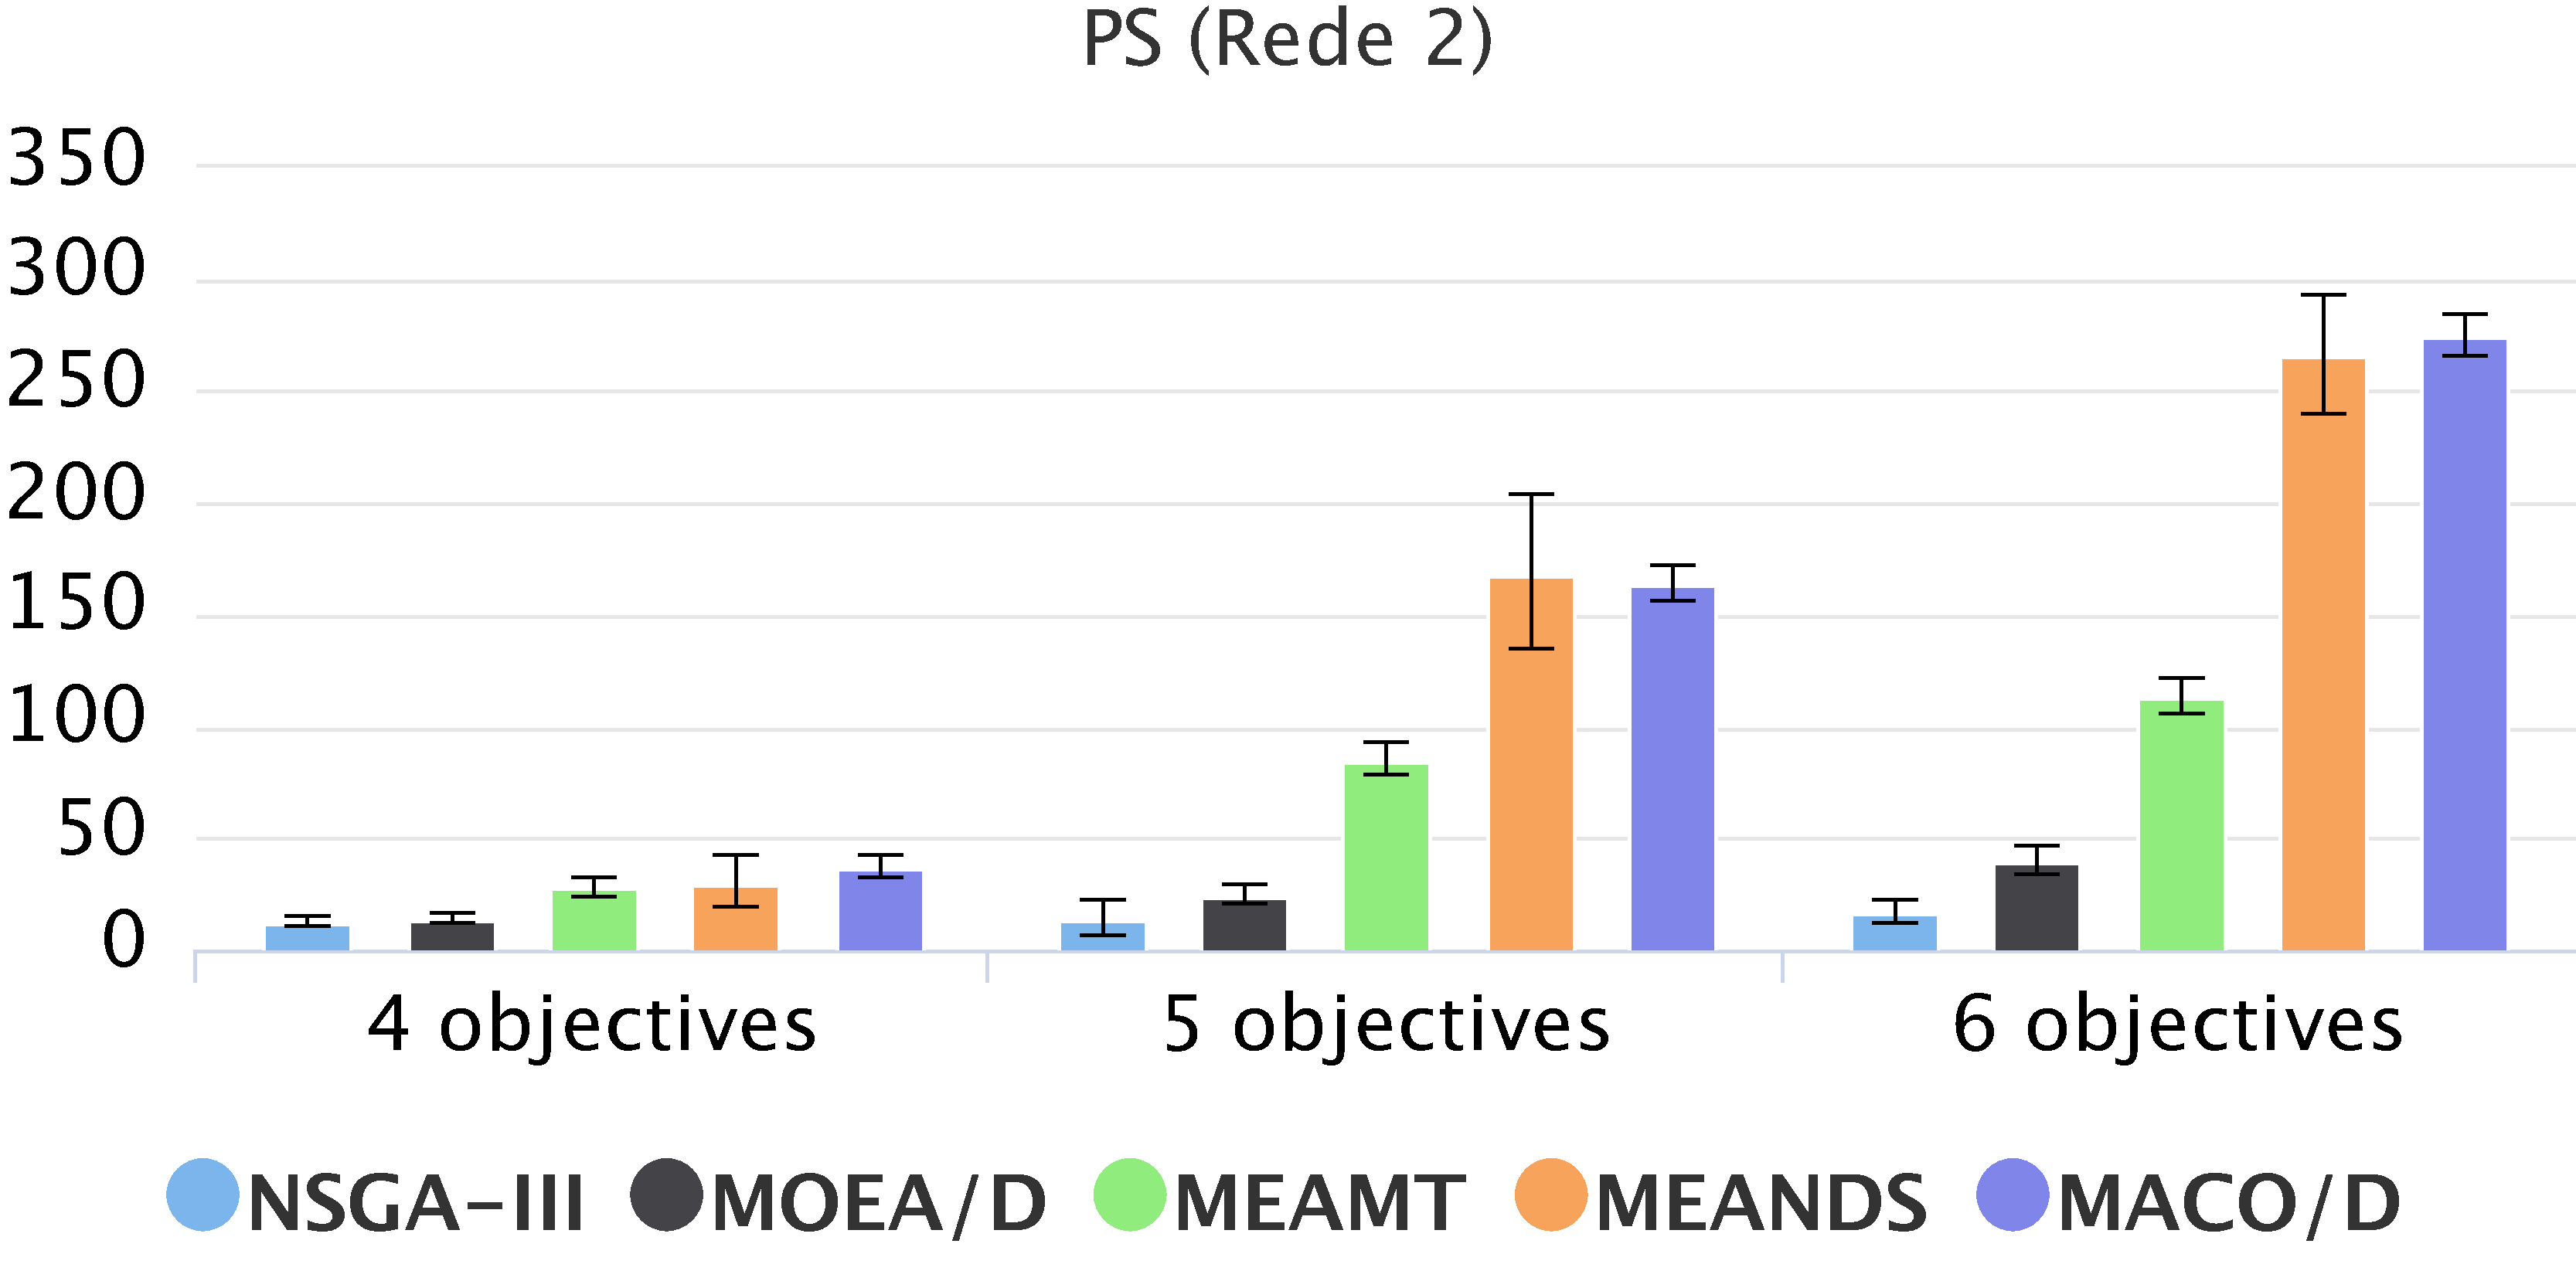
\includegraphics[width=0.5\textwidth]{cap_experimentos/figs/etapa2/ps-mrp-r2}
	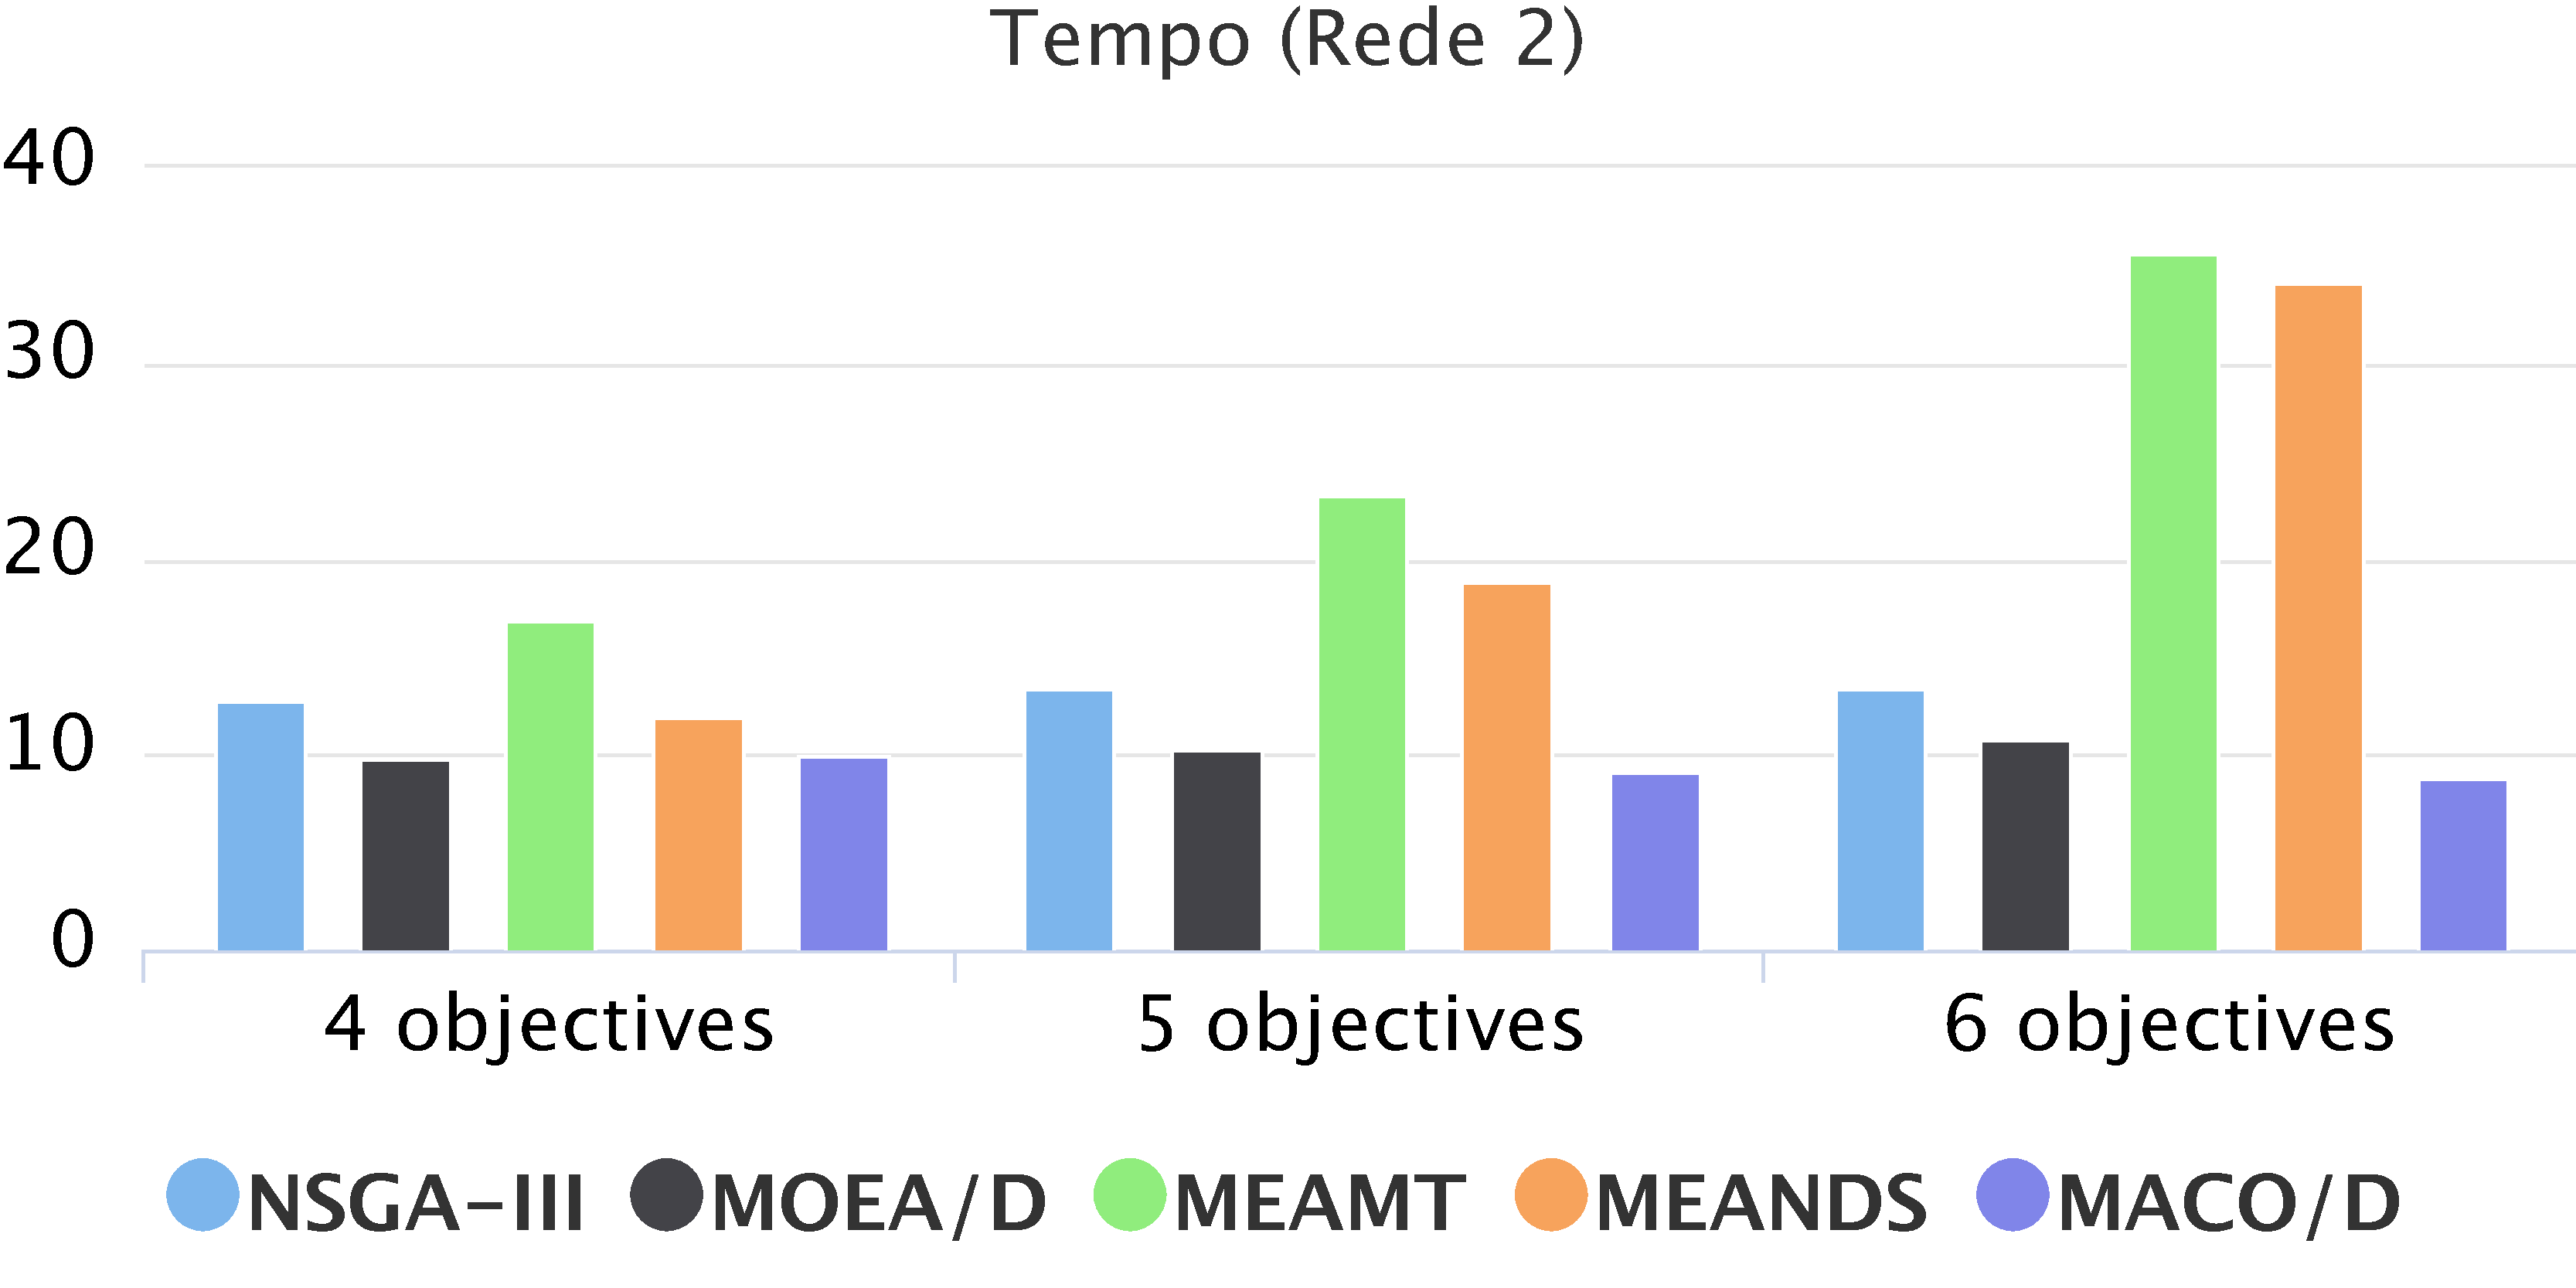
\includegraphics[width=0.5\textwidth]{cap_experimentos/figs/etapa2/time-mrp-r2}
\end{figure*}

Análise do PRM-R2

\begin{figure*}[!htbp]
	\caption{Etapa 2: resultados para o PRM na rede $R_3$}
	\label{fig_exp2_mrp_r3}
	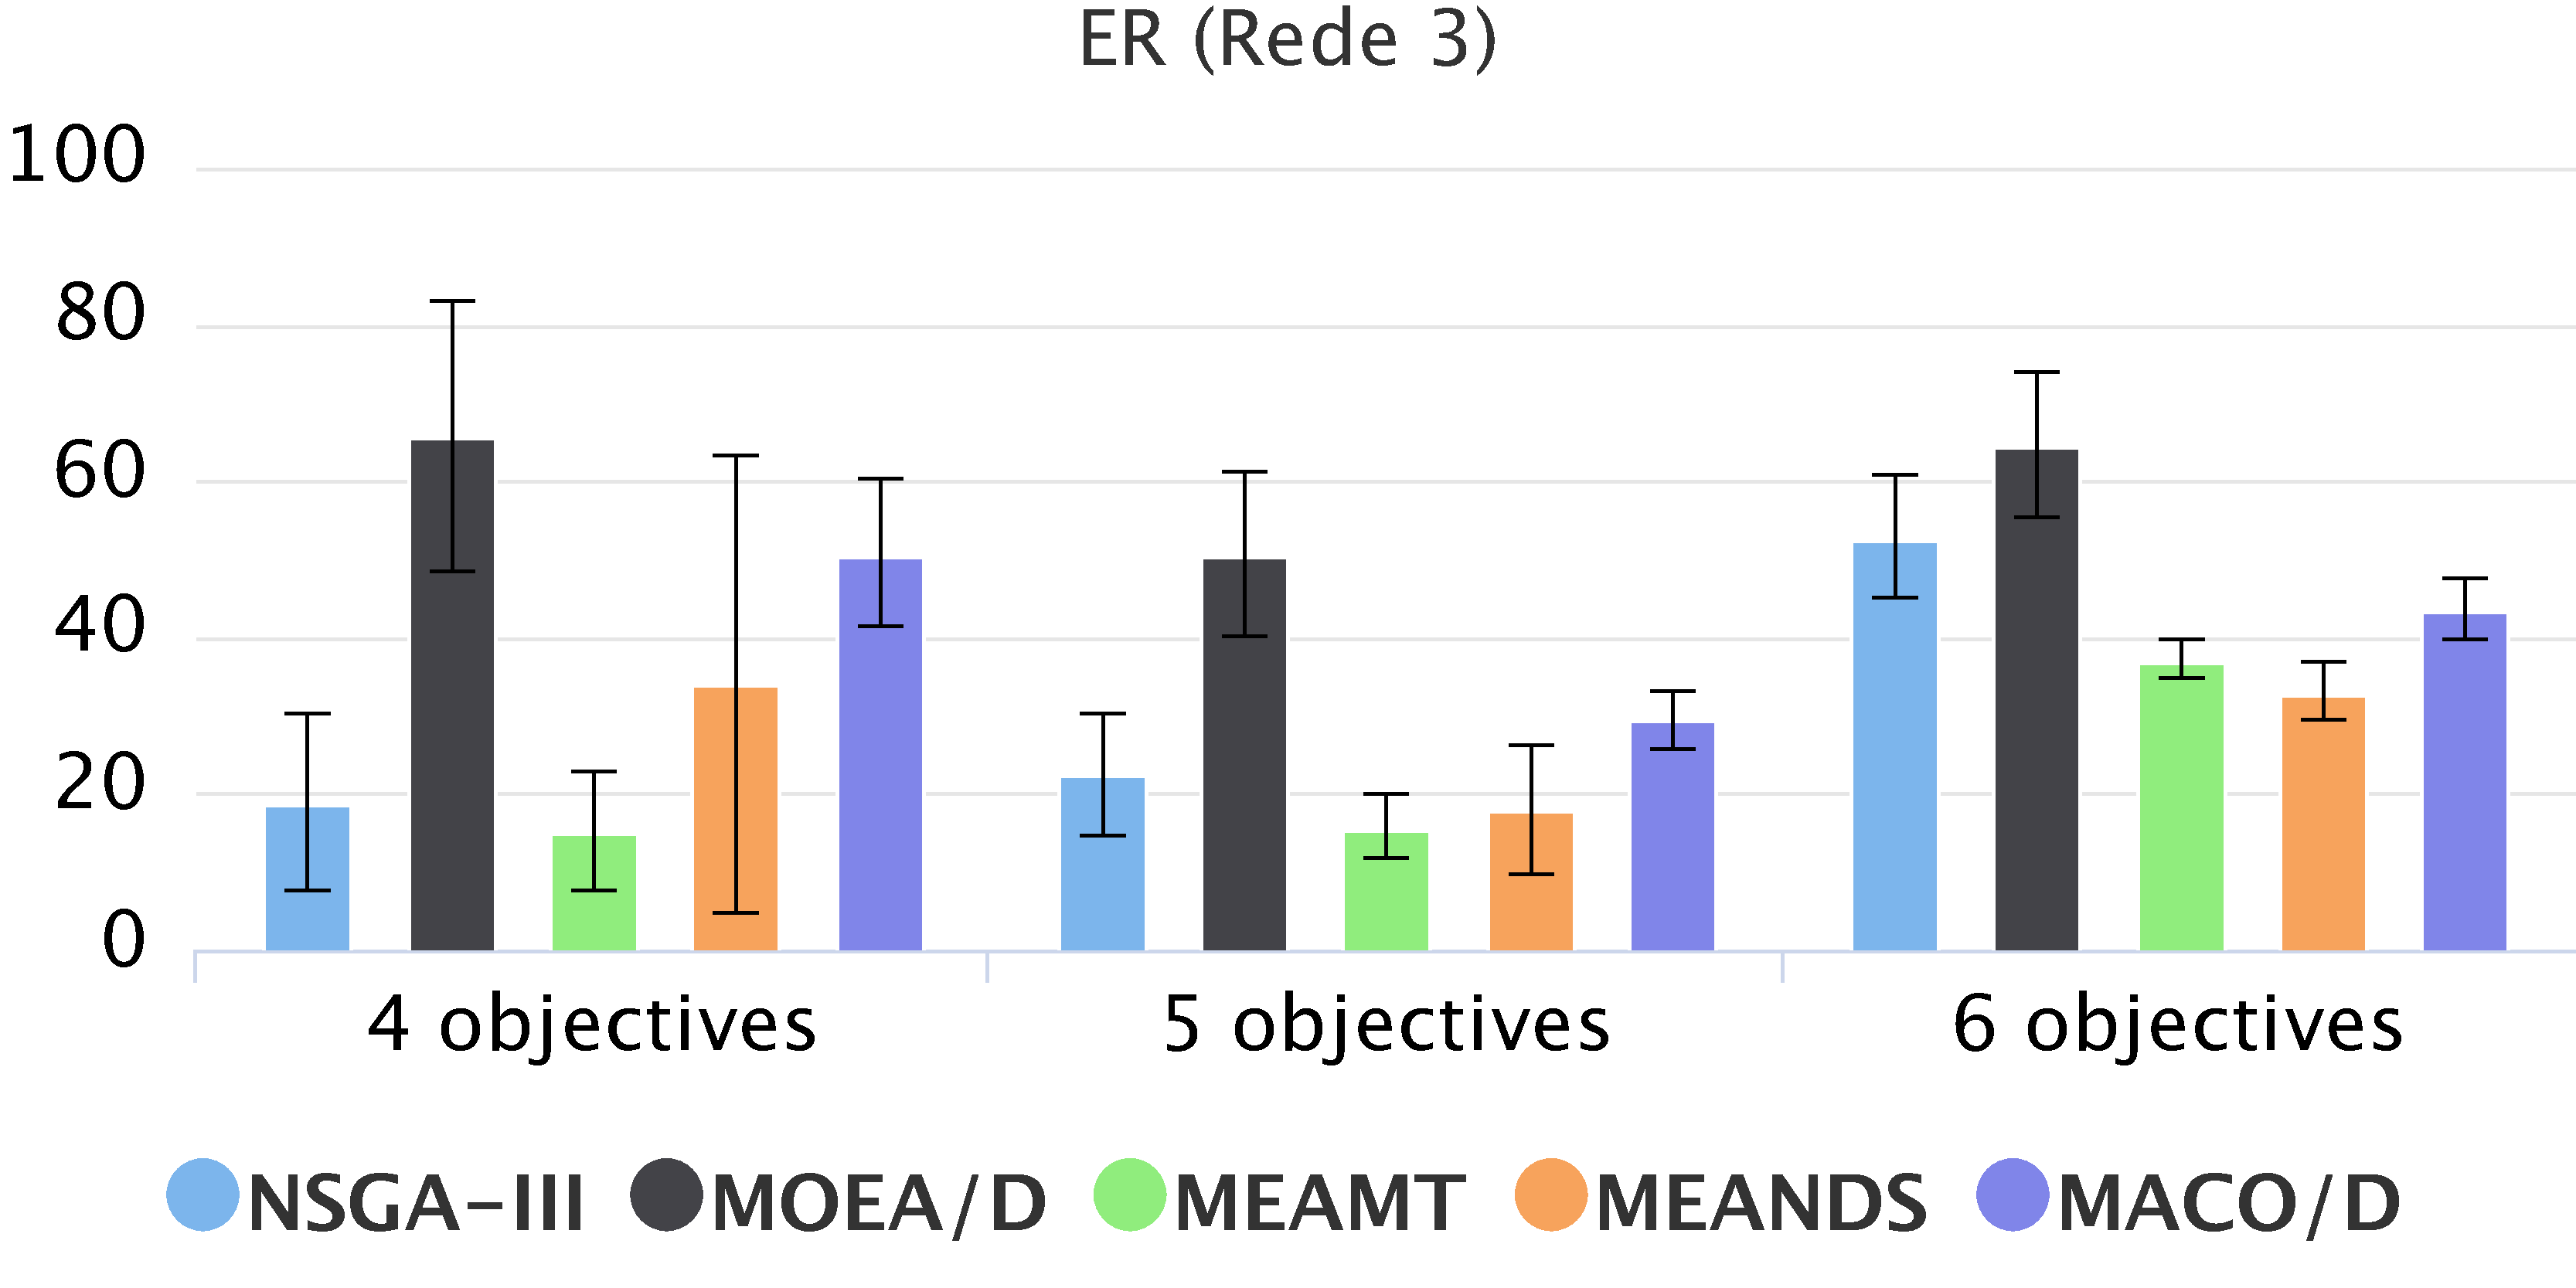
\includegraphics[width=0.5\textwidth]{cap_experimentos/figs/etapa2/er-mrp-r3}
	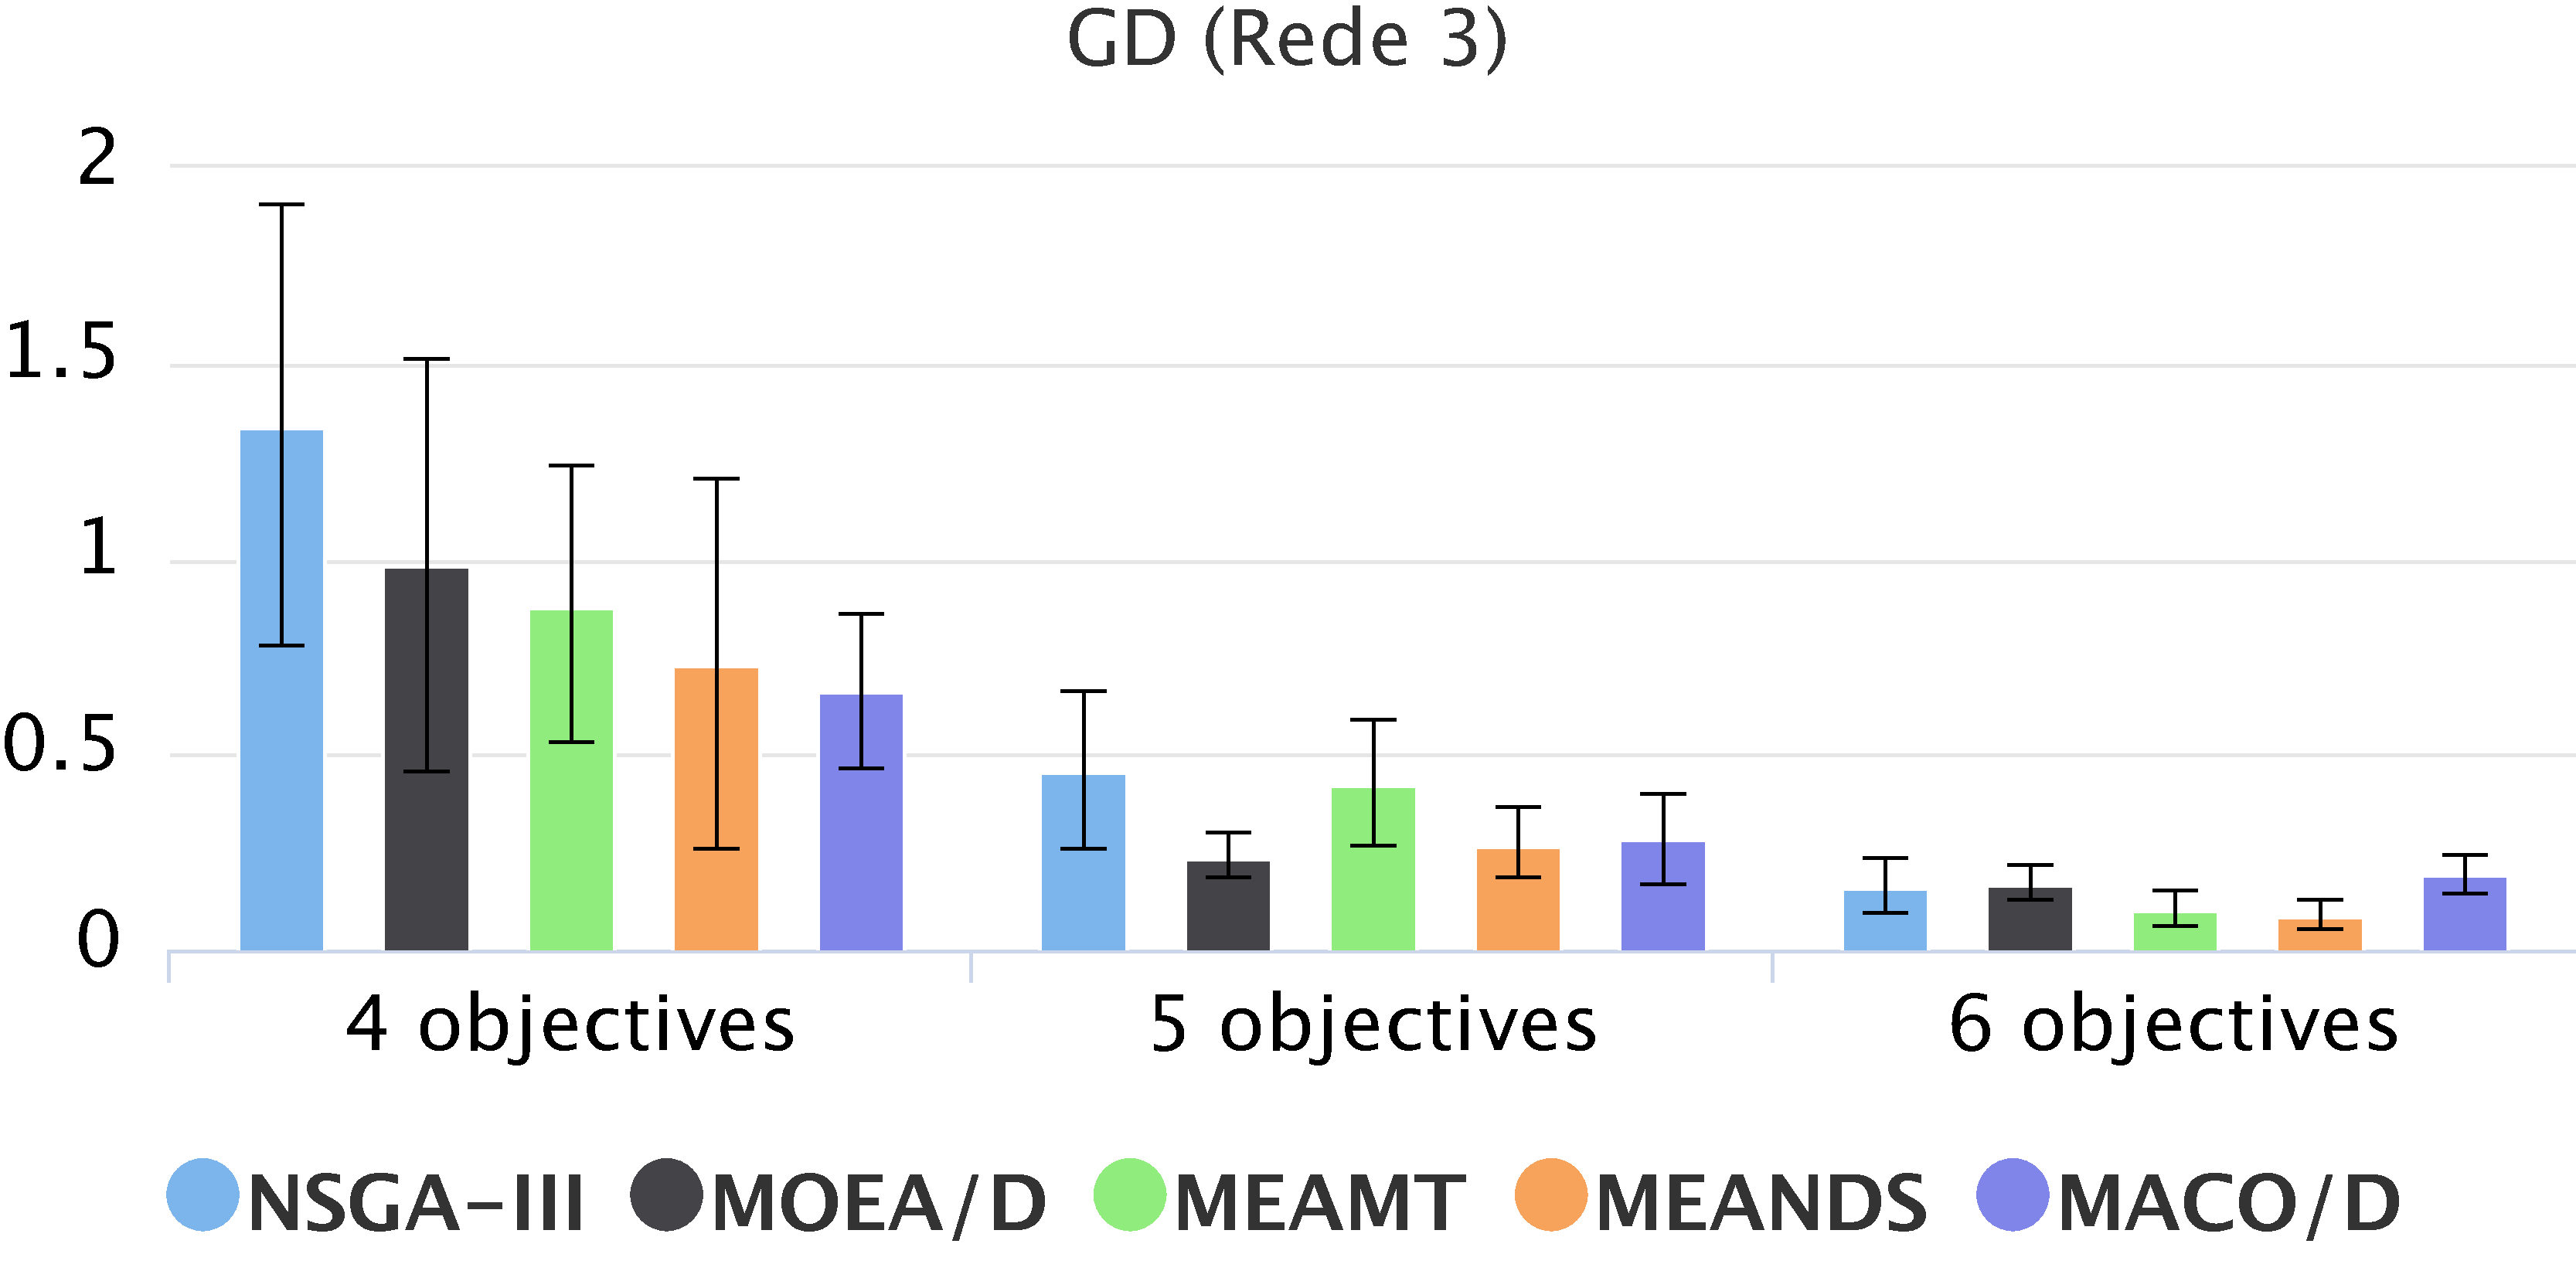
\includegraphics[width=0.5\textwidth]{cap_experimentos/figs/etapa2/gd-mrp-r3}
	\includegraphics[width=0.5\textwidth]{cap_experimentos/figs/etapa2/ps-mrp-r3}
	\includegraphics[width=0.5\textwidth]{cap_experimentos/figs/etapa2/time-mrp-r3}
\end{figure*}

Análise do PRM-R3

\begin{figure*}[!htbp]
	\caption{Etapa 2: resultados agrupados para o PRM nas redes $R_1$, $R_2$ e $R_3$}
	\label{fig_exp2_mrp_todos}
	\includegraphics[width=0.5\textwidth]{cap_experimentos/figs/etapa2/er-mrp-todos}
	\includegraphics[width=0.5\textwidth]{cap_experimentos/figs/etapa2/gd-mrp-todos}
	\includegraphics[width=0.5\textwidth]{cap_experimentos/figs/etapa2/ps-mrp-todos}
	\includegraphics[width=0.5\textwidth]{cap_experimentos/figs/etapa2/time-mrp-todos}
\end{figure*}

Análise geral do PRM

Análise geral dos resultados comparando os dois problemas.

\section{Etapa 3: Análise com hipervolume}

A fim de testar propriamente o comportamento dos algoritmos em espaços de busca mais complexos que os utilizados nos experimentos das etapas 1 e 2, lançou-se mão de três novas redes e instâncias do problema da mochila com 100 e 200 itens. Como não é possível extrair Paretos estáveis para as redes $R_4$, $R_5$ e $R_6$, nem para os problemas da mochila com 50, 100 e 200 itens, não é interessante basear-se em métricas dependentes de tais Paretos para se tirar conclusões. Por isso, nesta etapa, testa-se unicamente a métrica hipervolume, independente do Pareto.

O hipervolume foi utilizado pela primeira vez em [] e desde então, junto a \textit{inverse generational distance} $(IDG)$ [], é a métrica mais utilizada na literatura para se avaliar algoritmos many-objectives. O hipervolume, como explicado no início deste capítulo, calcula o volume da figura geométrica formada pelas distâncias das soluções a um ponto de referência pré-definido. Os pontos de referência utilizados em cada cenário são apresentados na tabela [].

Tabela de pontos de referência.

Nesta etapa testou-se os algoritmos NSGA-III, SPEA2-SDE, MOEA/D, AEMMT, AEMMD, MOACS e MACO/D. Foram 3 formulações de objetivo para cada problema (4, 5 e 6 objetivos) e 3 instâncias, totalizando 18 cenários de teste. Foram realizadas 10 execuções para cada algoritmo em cada cenário e os resultados foram calculados através das médias dos hivervolumes de cada execução.

Falar sobre figuras.
Exibir figuras.
Discutir resultados.